% Options for packages loaded elsewhere
\PassOptionsToPackage{unicode}{hyperref}
\PassOptionsToPackage{hyphens}{url}
\PassOptionsToPackage{dvipsnames,svgnames*,x11names*}{xcolor}
%
\documentclass[
  12pt,
]{krantz}
\usepackage{lmodern}
\usepackage{amssymb,amsmath}
\usepackage{ifxetex,ifluatex}
\ifnum 0\ifxetex 1\fi\ifluatex 1\fi=0 % if pdftex
  \usepackage[T1]{fontenc}
  \usepackage[utf8]{inputenc}
  \usepackage{textcomp} % provide euro and other symbols
\else % if luatex or xetex
  \usepackage{unicode-math}
  \defaultfontfeatures{Scale=MatchLowercase}
  \defaultfontfeatures[\rmfamily]{Ligatures=TeX,Scale=1}
\fi
% Use upquote if available, for straight quotes in verbatim environments
\IfFileExists{upquote.sty}{\usepackage{upquote}}{}
\IfFileExists{microtype.sty}{% use microtype if available
  \usepackage[]{microtype}
  \UseMicrotypeSet[protrusion]{basicmath} % disable protrusion for tt fonts
}{}
\makeatletter
\@ifundefined{KOMAClassName}{% if non-KOMA class
  \IfFileExists{parskip.sty}{%
    \usepackage{parskip}
  }{% else
    \setlength{\parindent}{0pt}
    \setlength{\parskip}{6pt plus 2pt minus 1pt}}
}{% if KOMA class
  \KOMAoptions{parskip=half}}
\makeatother
\usepackage{xcolor}
\IfFileExists{xurl.sty}{\usepackage{xurl}}{} % add URL line breaks if available
\IfFileExists{bookmark.sty}{\usepackage{bookmark}}{\usepackage{hyperref}}
\hypersetup{
  pdftitle={Interpretable Machine Learning},
  pdfauthor={Christoph Molnar},
  colorlinks=true,
  linkcolor=Maroon,
  filecolor=Maroon,
  citecolor=Blue,
  urlcolor=Blue,
  pdfcreator={LaTeX via pandoc}}
\urlstyle{same} % disable monospaced font for URLs
\usepackage{longtable,booktabs}
% Correct order of tables after \paragraph or \subparagraph
\usepackage{etoolbox}
\makeatletter
\patchcmd\longtable{\par}{\if@noskipsec\mbox{}\fi\par}{}{}
\makeatother
% Allow footnotes in longtable head/foot
\IfFileExists{footnotehyper.sty}{\usepackage{footnotehyper}}{\usepackage{footnote}}
\makesavenoteenv{longtable}
\usepackage{graphicx,grffile}
\makeatletter
\def\maxwidth{\ifdim\Gin@nat@width>\linewidth\linewidth\else\Gin@nat@width\fi}
\def\maxheight{\ifdim\Gin@nat@height>\textheight\textheight\else\Gin@nat@height\fi}
\makeatother
% Scale images if necessary, so that they will not overflow the page
% margins by default, and it is still possible to overwrite the defaults
% using explicit options in \includegraphics[width, height, ...]{}
\setkeys{Gin}{width=\maxwidth,height=\maxheight,keepaspectratio}
% Set default figure placement to htbp
\makeatletter
\def\fps@figure{htbp}
\makeatother
\setlength{\emergencystretch}{3em} % prevent overfull lines
\providecommand{\tightlist}{%
  \setlength{\itemsep}{0pt}\setlength{\parskip}{0pt}}
\setcounter{secnumdepth}{5}
% to allow chinese characters
%\usepackage[UTF8]{ctex}

% dont show rmdnotes
\newenvironment{rmdnote}{}{}


% Decide for a font
\usepackage{Alegreya}
\usepackage[scale=.7]{sourcecodepro}


% Make stuff less floaty
\renewcommand{\textfraction}{0.05}
\renewcommand{\topfraction}{0.8}
\renewcommand{\bottomfraction}{0.8}
\renewcommand{\floatpagefraction}{0.75}

% Turns href urls into foodnotes
\let\oldhref\href
\renewcommand{\href}[2]{#2\footnote{\url{#1}}}

% Create index
\usepackage{makeidx}
\makeindex

% Pages for publishing, like empty pages
\frontmatter
\usepackage{booktabs}
\usepackage{longtable}
\usepackage{array}
\usepackage{multirow}
\usepackage{wrapfig}
\usepackage{float}
\usepackage{colortbl}
\usepackage{pdflscape}
\usepackage{tabu}
\usepackage{threeparttable}
\usepackage{threeparttablex}
\usepackage[normalem]{ulem}
\usepackage{makecell}
\usepackage{xcolor}

\title{Interpretable Machine Learning}
\usepackage{etoolbox}
\makeatletter
\providecommand{\subtitle}[1]{% add subtitle to \maketitle
  \apptocmd{\@title}{\par {\large #1 \par}}{}{}
}
\makeatother
\subtitle{A Guide for Making Black Box Models Explainable.}
\author{Christoph Molnar}
\date{2021-10-09}

\begin{document}
\maketitle

%\cleardoublepage\newpage\thispagestyle{empty}\null
%\cleardoublepage\newpage\thispagestyle{empty}\null
%\cleardoublepage\newpage
\thispagestyle{empty}
%\begin{center}
%\includegraphics{images/dedication.pdf}
%\end{center}

\setlength{\abovedisplayskip}{-5pt}
\setlength{\abovedisplayshortskip}{-5pt}

{
\hypersetup{linkcolor=}
\setcounter{tocdepth}{1}
\tableofcontents
}
\listoftables
\listoffigures
\hypertarget{summary}{%
\chapter*{Summary}\label{summary}}


Machine learning has great potential for improving products, processes and research.
But \textbf{computers usually do not explain their predictions} which is a barrier to the adoption of machine learning.
This book is about making machine learning models and their decisions interpretable.

After exploring the concepts of interpretability, you will learn about simple, \textbf{interpretable models} such as decision trees, decision rules and linear regression.
The focus of the book is on model-agnostic methods for \textbf{interpreting black box models} such as feature importance and accumulated local effects, and explaining individual predictions with Shapley values and LIME.
In addition, the book presents methods specific to deep neural networks.

All interpretation methods are explained in depth and discussed critically.
How do they work under the hood?
What are their strengths and weaknesses?
How can their outputs be interpreted?
This book will enable you to select and correctly apply the interpretation method that is most suitable for your machine learning project.
Reading the book is recommended for machine learning practitioners, data scientists, statisticians, and anyone else interested in making machine learning models interpretable.

\textbf{About me:} My name is Christoph Molnar, I'm a statistician and a machine learner.
My goal is to make machine learning interpretable.

Follow me on Twitter! \href{https://twitter.com/ChristophMolnar}{@ChristophMolnar}

Cover by \href{https://twitter.com/YvonneDoinel}{@YvonneDoinel}

\begin{figure}

{\centering \includegraphics[width=\textwidth]{images/by-nc-sa} 

}

\end{figure}

This book is licensed under the \href{http://creativecommons.org/licenses/by-nc-sa/4.0/}{Creative Commons Attribution-NonCommercial-ShareAlike 4.0 International License}.

\hypertarget{preface-by-the-author}{%
\chapter{Preface by the Author}\label{preface-by-the-author}}

This book started as a side project when I was working as a statistician in clinical research.
I worked 4 days a week, and on my ``day off'' I worked on side projects.
Eventually, interpretable machine learning became one of my side projects.
At first I had no intention of writing a book.
Instead, I was simply interested in finding out more about interpretable machine learning and was looking for good resources to learn from.
Given the success of machine learning and the importance of interpretability, I expected that there would be tons of books and tutorials on this topic.
But I only found the relevant research papers and a few blog posts scattered around the internet, but nothing with a good overview.
No books, no tutorials, no overview papers, nothing.
This gap inspired me to start this book.
I ended up writing the book I wished was available when I began my study of interpretable machine learning.
My intention with this book was twofold: to learn for myself and to share this new knowledge with others.

I received my bachelor's and master's degree in statistics at the LMU Munich, Germany.
Most of my knowledge about machine learning was self-taught through online courses, competitions, side projects and professional activities.
My statistical background was an excellent basis for getting into machine learning, and especially for interpretability.
In statistics, a major focus is on building interpretable regression models.
After I finished my master's degree in statistics, I decided not to pursue a PhD, because I did not enjoy writing my master's thesis.
Writing just stressed me out too much.
So I took jobs as data scientist in a Fintech start-up and as statistician in clinical research.
After these three years in industry I started writing this book and a few months later I started a PhD in interpretable machine learning.
By starting this book, I regained the joy of writing and it helped me to develop a passion for research.

This book covers many techniques of interpretable machine learning.
In the first chapters I introduce the concept of interpretability and motivate why interpretability is necessary.
There are even some short stories!
The book discusses the different properties of explanations and what humans think is a good explanation.
Then we will discuss machine learning models that are inherently interpretable, for example regression models and decision trees.
The main focus of this book is on model-agnostic interpretability methods.
Model-agnostic means that these methods can be applied to any machine learning model and are applied after the model has been trained.
The independence of the model makes model-agnostic methods very flexible and powerful.
Some techniques explain how individual predictions were made, like local interpretable model-agnostic explanations (LIME) and Shapley values.
Other techniques describe the average behavior of the model across a dataset.
Here we learn about the partial dependence plot, accumulated local effects, permutation feature importance and many other methods.
A special category are example-based methods that produce data points as explanations.
Counterfactual explanations, prototypes, influential instances and adversarial examples are example-based methods that are discussed in this book.
The book concludes with some reflections on what the future of interpretable machine learning might look like.

You do not have to read the book from cover to cover, you can jump back and forth and concentrate on the techniques that interest you most.
I only recommend that you start with the introduction and the chapter on interpretability.
Most chapters follow a similar structure and focus on one interpretation method.
The first paragraph summarizes the method.
Then I try to explain the method intuitively without relying on mathematical formulas.
Then we look at the theory of the method to get a deep understanding of how it works.
You will not be spared here, because the theory will contain formulas.
I believe that a new method is best understood using examples.
Therefore, each method is applied to real data.
Some people say that statistician are very critical people.
For me, this is true, because each chapter contains critical discussions about advantages and disadvantages of the respective interpretation method.
This book is not an advertisement for the methods, but it should help you decide whether a method works well for your application or not.
In the last section of each chapter, available software implementations are discussed.

Machine learning has received great attention from many people in research and industry.
Sometimes machine learning is overhyped in the media, but there are many real and impactful applications.
Machine learning is a powerful technology for products, research and automation.
Today machine learning is used, for example, to detect fraudulent financial transactions, recommend movies to watch and classify images.
It is often crucial that the machine learning models are interpretable.
Interpretability helps the developer to debug and improve the model, build trust in the model, justify model predictions and gain insights.
The increased need for machine learning interpretability is a natural consequence of an increased use of machine learning.
This book has become a valuable resource for many people.
Teaching instructors use the book to introduce their students to the concepts of interpretable machine learning.
I received e-mails from various master and doctoral students who told me that this book was the starting point and most important reference for their theses.
The book has helped applied researchers in the field of ecology, finance, psychology, etc. who use machine learning to understand their data.
Data scientists from industry told me that they use the ``Interpretable Machine Learning'' book for their work and recommend it to their colleagues.
I am happy that many people can benefit from this book and become experts in model interpretation.

I would recommend this book to practitioners who want an overview of techniques to make their machine learning models more interpretable.
It is also recommended to students and researchers (and anyone else) who is interested in the topic.
To benefit from this book, you should already have a basic understanding of machine learning.
You should also have a mathematical understanding at university entry level to be able to follow the theory and formulas in this book.
It should also be possible, however, to understand the intuitive description of the method at the beginning of each chapter without mathematics.

I hope you enjoy the book!

\mainmatter

\hypertarget{intro}{%
\chapter{Introduction}\label{intro}}

This book explains to you how to make (supervised) machine learning models interpretable.
The chapters contain some mathematical formulas, but you should be able to understand the ideas behind the methods even without the formulas.
This book is not for people trying to learn machine learning from scratch.
If you are new to machine learning, there are a lot of books and other resources to learn the basics.
I recommend the book ``The Elements of Statistical Learning'' by Hastie, Tibshirani, and Friedman (2009) \footnote{Friedman, Jerome, Trevor Hastie, and Robert Tibshirani. ``The elements of statistical learning''. www.web.stanford.edu/\textasciitilde hastie/ElemStatLearn/ (2009).} and \href{https://www.coursera.org/learn/machine-learning}{Andrew Ng's ``Machine Learning'' online course} on the online learning platform coursera.com to start with machine learning.
Both the book and the course are available free of charge!

New methods for the interpretation of machine learning models are published at breakneck speed.
To keep up with everything that is published would be madness and simply impossible.
That is why you will not find the most novel and fancy methods in this book, but established methods and basic concepts of machine learning interpretability.
These basics prepare you for making machine learning models interpretable.
Internalizing the basic concepts also empowers you to better understand and evaluate any new paper on interpretability published on \href{https://arxiv.org/}{arxiv.org} in the last 5 minutes since you began reading this book (I might be exaggerating the publication rate).

This book starts with some (dystopian) \protect\hyperlink{storytime}{short stories} that are not needed to understand the book, but hopefully will entertain and make you think.
Then the book explores the concepts of \protect\hyperlink{interpretability}{machine learning interpretability}.
We will discuss when interpretability is important and what different types of explanations there are.
Terms used throughout the book can be looked up in the \protect\hyperlink{terminology}{Terminology chapter}.
Most of the models and methods explained are presented using real data examples which are described in the \protect\hyperlink{data}{Data chapter}.
One way to make machine learning interpretable is to use \protect\hyperlink{simple}{interpretable models}, such as linear models or decision trees.
The other option is the use of \protect\hyperlink{agnostic}{model-agnostic interpretation tools} that can be applied to any supervised machine learning model.
Model-agnostic methods can be divided \protect\hyperlink{global-methods}{global methods} that describe the average behavior of the model and \protect\hyperlink{local-methods}{local methods} that explain individual predictions.
The Model-Agnostic Methods chapter deals with methods such as \protect\hyperlink{pdp}{partial dependence plots} and \protect\hyperlink{feature-importance}{feature importance}.
Model-agnostic methods work by changing the input of the machine learning model and measuring changes in the prediction output.
The book ends with an optimistic outlook on what \protect\hyperlink{future}{the future of interpretable machine learning} might look like.

You can either read the book from beginning to end or jump directly to the methods that interest you.

I hope you will enjoy the read!

\newpage

\hypertarget{storytime}{%
\section{Story Time}\label{storytime}}

We will start with some short stories.
Each story is an admittedly exaggerated call for interpretable machine learning.
If you are in a hurry, you can skip the stories.
If you want to be entertained and (de-)motivated, read on!

The format is inspired by Jack Clark's Tech Tales in his \href{https://jack-clark.net/}{Import AI Newsletter}.
If you like this kind of stories or if you are interested in AI, I recommend that you sign up.

\hypertarget{lightning-never-strikes-twice}{%
\subsection*{Lightning Never Strikes Twice}\label{lightning-never-strikes-twice}}


\textbf{2030: A medical lab in Switzerland}

\begin{figure}

{\centering \includegraphics[width=\textwidth]{images/hospital} 

}

\end{figure}

``It's definitely not the worst way to die!'' Tom summarised, trying to find something positive in the tragedy.
He removed the pump from the intravenous pole.\\
``He just died for the wrong reasons,'' Lena added.\\
``And certainly with the wrong morphine pump!
Just creating more work for us!'' Tom complained while unscrewing the back plate of the pump.
After removing all the screws, he lifted the plate and put it aside.
He plugged a cable into the diagnostic port.\\
``You didn't just complain about having a job, did you?'' Lena gave him a mocking smile.\\
``Of course not. Never!'' he exclaimed with a sarcastic undertone.

He booted the pump's computer.\\
Lena plugged the other end of the cable into her tablet.
``All right, diagnostics are running,'' she announced.
``I am really curious about what went wrong.''\\
``It certainly shot our John Doe into Nirvana.
That high concentration of this morphine stuff.
Man. I mean \ldots{} that's a first, right?
Normally a broken pump gives off too little of the sweet stuff or nothing at all.
But never, you know, like that crazy shot,'' Tom explained.\\
``I know. You don't have to convince me \ldots{} Hey, look at that.'' Lena held up her tablet.
``Do you see this peak here? That's the potency of the painkillers mix.
Look! This line shows the reference level.
The poor guy had a mixture of painkillers in his blood system that could kill him 17 times over.
Injected by our pump here.
And here \ldots{}'' she swiped, ``here you can see the moment of the patient's demise.''\\
``So, any idea what happened, boss?'' Tom asked his supervisor.\\
``Hm \ldots{} The sensors seem to be fine.
Heart rate, oxygen levels, glucose, \ldots{} The data were collected as expected.
Some missing values in the blood oxygen data, but that's not unusual.
Look here.
The sensors have also detected the patient's slowing heart rate and extremely low cortisol levels caused by the morphine derivate and other pain blocking agents.''
She continued to swipe through the diagnostics report.\\
Tom stared captivated at the screen.
It was his first investigation of a real device failure.

``Ok, here is our first piece of the puzzle.
The system failed to send a warning to the hospital's communication channel.
The warning was triggered, but rejected at protocol level.
It could be our fault, but it could also be the fault of the hospital.
Please send the logs over to the IT team,'' Lena told Tom.\\
Tom nodded with his eyes still fixed on the screen.\\
Lena continued:
``It's odd.
The warning should also have caused the pump to shut down.
But it obviously failed to do so.
That must be a bug.
Something the quality team missed.
Something really bad.
Maybe it's related to the protocol issue.''\\
``So, the emergency system of the pump somehow broke down, but why did the pump go full bananas and inject so much painkiller into John Doe?'' Tom wondered.\\
``Good question.
You are right.
Protocol emergency failure aside, the pump shouldn't have administered that amount of medication at all.
The algorithm should have stopped much earlier on its own, given the low level of cortisol and other warning signs,'' Lena explained.\\
``Maybe some bad luck, like a one in a million thing, like being hit by a lightning?'' Tom asked her.\\
``No, Tom.
If you had read the documentation I sent you, you would have known that the pump was first trained in animal experiments, then later on humans, to learn to inject the perfect amount of painkillers based on the sensory input.
The algorithm of the pump might be opaque and complex, but it's not random.
That means that in the same situation the pump would behave exactly the same way again.
Our patient would die again.
A combination or undesired interaction of the sensory inputs must have triggered the erroneous behavior of the pump.
That is why we have to dig deeper and find out what happened here,'' Lena explained.

``I see \ldots,'' Tom replied, lost in thought.
``Wasn't the patient going to die soon anyway? Because of cancer or something?''\\
Lena nodded while she read the analysis report.\\
Tom got up and went to the window.
He looked outside, his eyes fixed on a point in the distance.
``Maybe the machine did him a favor, you know, in freeing him from the pain.
No more suffering.
Maybe it just did the right thing.
Like a lightning, but, you know, a good one.
I mean like the lottery, but not random.
But for a reason.
If I were the pump, I would have done the same.''\\
She finally lifted her head and looked at him.\\
He kept looking at something outside.\\
Both were silent for a few moments.\\
Lena lowered her head again and continued the analysis.
``No, Tom. It's a bug\ldots{} Just a damn bug.''

\hypertarget{trust-fall}{%
\subsection*{Trust Fall}\label{trust-fall}}


\textbf{2050: A subway station in Singapore}

\begin{figure}

{\centering \includegraphics[width=\textwidth]{images/access-denied} 

}

\end{figure}

She rushed to the Bishan subway station.
With her thoughts she was already at work.
The tests for the new neural architecture should be completed by now.
She led the redesign of the government's ``Tax Affinity Prediction System for Individual Entities'', which predicts whether a person will hide money from the tax office.
Her team has come up with an elegant piece of engineering.
If successful, the system would not only serve the tax office, but also feed into other systems such as the counter-terrorism alarm system and the commercial registry.
One day, the government could even integrate the predictions into the Civic Trust Score.
The Civic Trust Score estimates how trustworthy a person is.
The estimate affects every part of your daily life, such as getting a loan or how long you have to wait for a new passport.
As she descended the escalator, she imagined how an integration of her team's system into the Civic Trust Score System might look like.

She routinely wiped her hand over the RFID reader without reducing her walking speed.
Her mind was occupied, but a dissonance of sensory expectations and reality rang alarm bells in her brain.

Too late.

Nose first she ran into the subway entrance gate and fell with her butt first to the ground.
The door was supposed to open, \ldots{} but it did not.
Dumbfounded, she stood up and looked at the screen next to the gate.
``Please try another time,'' suggested a friendly looking smiley on the screen.
A person passed by and, ignoring her, wiped his hand over the reader.
The door opened and he went through.
The door closed again.
She wiped her nose.
It hurt, but at least it did not bleed.
She tried to open the door, but was rejected again.
It was strange.
Maybe her public transport account did not have sufficient tokens.
She looked at her smartwatch to check the account balance.

``Login denied. Please contact your Citizens Advice Bureau!'' her watch informed her.

A feeling of nausea hit her like a fist to the stomach.
She suspected what had happened.
To confirm her theory, she started the mobile game ``Sniper Guild'', an ego shooter.
The app was directly closed again automatically, which confirmed her theory.
She became dizzy and sat down on the floor again.

There was only one possible explanation:
Her Civic Trust Score had dropped.
Substantially.
A small drop meant minor inconveniences, such as not getting first class flights or having to wait a little longer for official documents.
A low trust score was rare and meant that you were classified as a threat to society.
One measure in dealing with these people was to keep them away from public places such as the subway.
The government restricted the financial transactions of subjects with low Civic Trust Scores.
They also began to actively monitor your behavior on social media and even went as far as to restrict certain content, such as violent games.
It became exponentially more difficult to increase your Civic Trust Score the lower it was.
People with a very low score usually never recovered.

She could not think of any reason why her score should have fallen.
The score was based on machine learning.
The Civic Trust Score System worked like a well-oiled engine that ran society.
The performance of the Trust Score System was always closely monitored.
Machine learning had become much better since the beginning of the century.
It had become so efficient that decisions made by the Trust Score System could no longer be disputed.
An infallible system.

She laughed in despair.
Infallible system.
If only.
The system has rarely failed.
But it failed.
She must be one of those special cases;
an error of the system;
from now on an outcast.
Nobody dared to question the system.
It was too integrated into the government, into society itself, to be questioned.
In the few remaining democratic countries it was forbidden to form anti-democratic movements, not because they where inherently malicious, but because they would destabilize the current system.
The same logic applied to the now more common algocraties.
Critique in the algorithms was forbidden because of the danger to the status quo.

Algorithmic trust was the fabric of the social order.
For the common good, rare false trust scorings were tacitly accepted.
Hundreds of other prediction systems and databases fed into the score, making it impossible to know what caused the drop in her score.
She felt like a big dark hole was opening in and under her.
With horror she looked into the void.

Her tax affinity system was eventually integrated into the Civic Trust Score System, but she never got to know it.

\hypertarget{fermis-paperclips}{%
\subsection*{Fermi's Paperclips}\label{fermis-paperclips}}


\textbf{Year 612 AMS (after Mars settlement): A museum on Mars}

\begin{figure}

{\centering \includegraphics[width=\textwidth]{images/burnt-earth} 

}

\end{figure}

``History is boring,'' Xola whispered to her friend.
Xola, a blue-haired girl, was lazily chasing one of the projector drones humming in the room with her left hand.
``History is important,'' the teacher said with an upset voice, looking at the girls.
Xola blushed.
She did not expect her teacher to overhear her.

``Xola, what did you just learn?'' the teacher asked her.
``That the ancient people used up all resources from Earther Planet and then died?'' she asked carefully.
``No.~They made the climate hot and it wasn't people, it was computers and machines. And it's Planet Earth, not Earther Planet,'' added another girl named Lin.
Xola nodded in agreement.
With a touch of pride, the teacher smiled and nodded.
``You are both right. Do you know why it happened?''
``Because people were short-sighted and greedy?'' Xola asked.
``People could not stop their machines!'' Lin blurted out.

``Again, you are both right,'' the teacher decided,
``but it's much more complicated than that.
Most people at the time were not aware of what was happening.
Some saw the drastic changes, but could not reverse them.
The most famous piece from this period is a poem by an anonymous author.
It best captures what happened at that time.
Listen carefully!''

The teacher started the poem.
A dozen of the small drones repositioned themselves in front of the children and began to project the video directly into their eyes.
It showed a person in a suit standing in a forest with only tree stumps left.
He began to talk:

\emph{The machines compute; the machines predict.}

\emph{We march on as we are part of it.}

\emph{We chase an optimum as trained.}

\emph{The optimum is one-dimensional, local and unconstrained.}

\emph{Silicon and flesh, chasing exponentiality.}

\emph{Growth is our mentality.}

\emph{When all rewards are collected,}

\emph{and side-effects neglected;}

\emph{When all the coins are mined,}

\emph{and nature has fallen behind;}

\emph{We will be in trouble,}

\emph{After all, exponential growth is a bubble.}

\emph{The tragedy of the commons unfolding,}

\emph{Exploding,}

\emph{Before our eyes.}

\emph{Cold calculations and icy greed,}

\emph{Fill the earth with heat.}

\emph{Everything is dying,}

\emph{And we are complying.}

\emph{Like horses with blinders we race the race of our own creation,}

\emph{Towards the Great Filter of civilization.}

\emph{And so we march on relentlessly.}

\emph{As we are part of the machine.}

\emph{Embracing entropy.}

``A dark memory,'' the teacher said to break the silence in the room.
``It will be uploaded to your library.
Your homework is to memorise it until next week.''
Xola sighed.
She managed to catch one of the little drones.
The drone was warm from the CPU and the engines.
Xola liked how it warmed her hands.

\newpage

\hypertarget{what-is-machine-learning}{%
\section{What Is Machine Learning?}\label{what-is-machine-learning}}

Machine learning is a set of methods that computers use to make and improve predictions or behaviors based on data.

For example, to predict the value of a house, the computer would learn patterns from past house sales.
The book focuses on supervised machine learning, which covers all prediction problems where we have a dataset for which we already know the outcome of interest (e.g.~past house prices) and want to learn to predict the outcome for new data.
Excluded from supervised learning are for example clustering tasks (= unsupervised learning) where we do not have a specific outcome of interest, but want to find clusters of data points.
Also excluded are things like reinforcement learning, where an agent learns to optimize a certain reward by acting in an environment (e.g.~a computer playing Tetris).
The goal of supervised learning is to learn a predictive model that maps features of the data (e.g.~house size, location, floor type, \ldots) to an output (e.g.~house price).
If the output is categorical, the task is called classification, and if it is numerical, it is called regression.
The machine learning algorithm learns a model by estimating parameters (like weights) or learning structures (like trees).
The algorithm is guided by a score or loss function that is minimized.
In the house value example, the machine minimizes the difference between the estimated house price and the predicted price.
A fully trained machine learning model can then be used to make predictions for new instances.

Estimation of house prices, product recommendations, street sign detection, credit default prediction and fraud detection:
All these examples have in common that they can be solved by machine learning.
The tasks are different, but the approach is the same:\\
Step 1: Data collection.
The more, the better.
The data must contain the outcome you want to predict and additional information from which to make the prediction.
For a street sign detector (``Is there a street sign in the image?''), you would collect street images and label whether a street sign is visible or not.
For a credit default predictor, you need past data on actual loans, information on whether the customers were in default with their loans, and data that will help you make predictions, such as income, past credit defaults, and so on.
For an automatic house value estimator program, you could collect data from past house sales and information about the real estate such as size, location, and so on.\\
Step 2: Enter this information into a machine learning algorithm that generates a sign detector model, a credit rating model or a house value estimator.\\
Step 3: Use model with new data.
Integrate the model into a product or process, such as a self-driving car, a credit application process or a real estate marketplace website.

Machines surpass humans in many tasks, such as playing chess (or more recently Go) or predicting the weather.
Even if the machine is as good as a human or a bit worse at a task, there remain great advantages in terms of speed, reproducibility and scaling.
A once implemented machine learning model can complete a task much faster than humans, reliably delivers consistent results and can be copied infinitely.
Replicating a machine learning model on another machine is fast and cheap.
The training of a human for a task can take decades (especially when they are young) and is very costly.
A major disadvantage of using machine learning is that insights about the data and the task the machine solves is hidden in increasingly complex models.
You need millions of numbers to describe a deep neural network, and there is no way to understand the model in its entirety.
Other models, such as the random forest, consist of hundreds of decision trees that ``vote'' for predictions.
To understand how the decision was made, you would have to look into the votes and structures of each of the hundreds of trees.
That just does not work no matter how clever you are or how good your working memory is.
The best performing models are often blends of several models (also called ensembles) that cannot be interpreted, even if each single model could be interpreted.
If you focus only on performance, you will automatically get more and more opaque models.
The winning models on machine learning competitions are often ensembles of models or very complex models such as boosted trees or deep neural networks.

\hypertarget{terminology}{%
\section{Terminology}\label{terminology}}

To avoid confusion due to ambiguity, here are some definitions of terms used in this book:

An \textbf{Algorithm} is a set of rules that a machine follows to achieve a particular goal\footnote{``Definition of Algorithm.'' \url{https://www.merriam-webster.com/dictionary/algorithm}. (2017).}.
An algorithm can be considered as a recipe that defines the inputs, the output and all the steps needed to get from the inputs to the output.
Cooking recipes are algorithms where the ingredients are the inputs, the cooked food is the output, and the preparation and cooking steps are the algorithm instructions.

\textbf{Machine Learning} is a set of methods that allow computers to learn from data to make and improve predictions (for example cancer, weekly sales, credit default).
Machine learning is a paradigm shift from ``normal programming'' where all instructions must be explicitly given to the computer to ``indirect programming'' that takes place through providing data.

\begin{figure}

{\centering \includegraphics[width=\textwidth]{images/programing-ml} 

}

\end{figure}

A \textbf{Learner} or \textbf{Machine Learning Algorithm} is the program used to learn a machine learning model from data.
Another name is ``inducer'' (e.g.~``tree inducer'').

A \textbf{Machine Learning Model} is the learned program that maps inputs to predictions.
This can be a set of weights for a linear model or for a neural network.
Other names for the rather unspecific word ``model'' are ``predictor'' or - depending on the task - ``classifier'' or ``regression model''.
In formulas, the trained machine learning model is called \(\hat{f}\) or \(\hat{f}(x)\).

\begin{figure}

{\centering 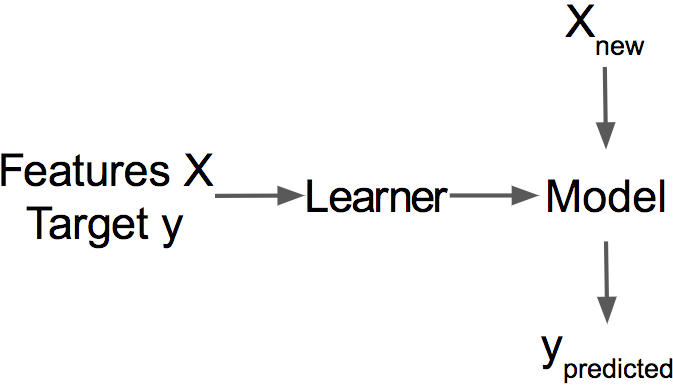
\includegraphics[width=\textwidth]{images/learner} 

}

\caption{A learner learns a model from labeled training data. The model is used to make predictions.}\label{fig:learner-definition}
\end{figure}

A \textbf{Black Box Model} is a system that does not reveal its internal mechanisms.
In machine learning, ``black box'' describes models that cannot be understood by looking at their parameters (e.g.~a neural network).
The opposite of a black box is sometimes referred to as \textbf{White Box}, and is referred to in this book as \protect\hyperlink{simple}{interpretable model}.
\protect\hyperlink{agnostic}{Model-agnostic methods} for interpretability treat machine learning models as black boxes, even if they are not.

\begin{figure}

{\centering 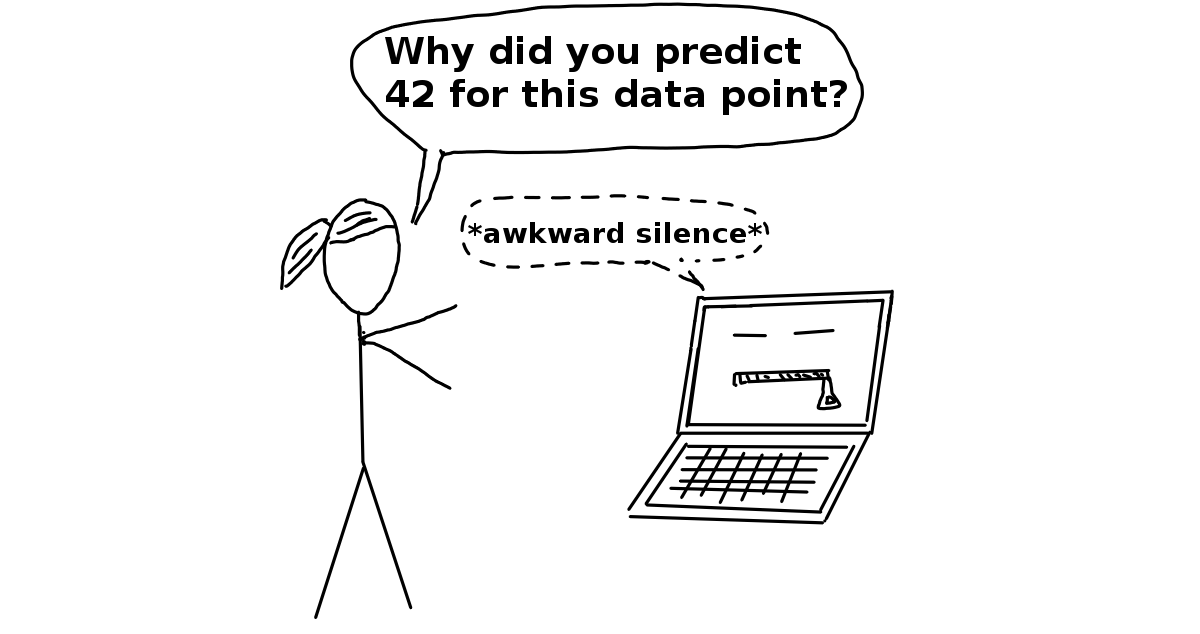
\includegraphics[width=\textwidth]{images/iml} 

}

\end{figure}

\textbf{Interpretable Machine Learning} refers to methods and models that make the behavior and predictions of machine learning systems understandable to humans.

A \textbf{Dataset} is a table with the data from which the machine learns.
The dataset contains the features and the target to predict.
When used to induce a model, the dataset is called training data.

An \textbf{Instance} is a row in the dataset.
Other names for `instance' are: (data) point, example, observation.
An instance consists of the feature values \(x^{(i)}\) and, if known, the target outcome \(y_i\).

The \textbf{Features} are the inputs used for prediction or classification.
A feature is a column in the dataset.
Throughout the book, features are assumed to be interpretable, meaning it is easy to understand what they mean, like the temperature on a given day or the height of a person.
The interpretability of the features is a big assumption.
But if it is hard to understand the input features, it is even harder to understand what the model does.
The matrix with all features is called X and \(x^{(i)}\) for a single instance.
The vector of a single feature for all instances is \(x_j\) and the value for the feature j and instance i is \(x^{(i)}_j\).

The \textbf{Target} is the information the machine learns to predict.
In mathematical formulas, the target is usually called y or \(y_i\) for a single instance.

A \textbf{Machine Learning Task} is the combination of a dataset with features and a target.
Depending on the type of the target, the task can be for example classification, regression, survival analysis, clustering, or outlier detection.

The \textbf{Prediction} is what the machine learning model ``guesses'' what the target value should be based on the given features.
In this book, the model prediction is denoted by \(\hat{f}(x^{(i)})\) or \(\hat{y}\).

\hypertarget{interpretability}{%
\chapter{Interpretability}\label{interpretability}}

There is no mathematical definition of interpretability.
A (non-mathematical) definition I like by Miller (2017)\footnote{Miller, Tim. ``Explanation in artificial intelligence: Insights from the social sciences.'' arXiv Preprint arXiv:1706.07269. (2017).} is:
\textbf{Interpretability is the degree to which a human can understand the cause of a decision.}
Another one is:
\textbf{Interpretability is the degree to which a human can consistently predict the model's result} \footnote{Kim, Been, Rajiv Khanna, and Oluwasanmi O. Koyejo. ``Examples are not enough, learn to criticize! Criticism for interpretability.'' Advances in Neural Information Processing Systems (2016).}.
The higher the interpretability of a machine learning model, the easier it is for someone to comprehend why certain decisions or predictions have been made.
A model is better interpretable than another model if its decisions are easier for a human to comprehend than decisions from the other model.
I will use both the terms interpretable and explainable interchangeably.
Like Miller (2017), I think it makes sense to distinguish between the terms interpretability/explainability and explanation.
I will use ``explanation'' for explanations of individual predictions.
See the \protect\hyperlink{explanation}{section about explanations} to learn what we humans see as a good explanation.

\hypertarget{interpretability-importance}{%
\section{Importance of Interpretability}\label{interpretability-importance}}

If a machine learning model performs well, \textbf{why do not we just trust the model} and ignore \textbf{why} it made a certain decision?
``The problem is that a single metric, such as classification accuracy, is an incomplete description of most real-world tasks.'' (Doshi-Velez and Kim 2017 \footnote{Doshi-Velez, Finale, and Been Kim. ``Towards a rigorous science of interpretable machine learning,'' no. Ml: 1--13. \url{http://arxiv.org/abs/1702.08608} ( 2017).})

Let us dive deeper into the reasons why interpretability is so important.
When it comes to predictive modeling, you have to make a trade-off:
Do you just want to know \textbf{what} is predicted?
For example, the probability that a customer will churn or how effective some drug will be for a patient.
Or do you want to know \textbf{why} the prediction was made and possibly pay for the interpretability with a drop in predictive performance?
In some cases, you do not care why a decision was made, it is enough to know that the predictive performance on a test dataset was good.
But in other cases, knowing the `why' can help you learn more about the problem, the data and the reason why a model might fail.
Some models may not require explanations because they are used in a low-risk environment, meaning a mistake will not have serious consequences, (e.g.~a movie recommender system) or the method has already been extensively studied and evaluated (e.g.~optical character recognition).
The need for interpretability arises from an incompleteness in problem formalization (Doshi-Velez and Kim 2017), which means that for certain problems or tasks it is not enough to get the prediction (the \textbf{what}).
The model must also explain how it came to the prediction (the \textbf{why}), because a correct prediction only partially solves your original problem.
The following reasons drive the demand for interpretability and explanations (Doshi-Velez and Kim 2017 and Miller 2017).

\textbf{Human curiosity and learning}: Humans have a mental model of their environment that is updated when something unexpected happens.
This update is performed by finding an explanation for the unexpected event.
For example, a human feels unexpectedly sick and asks, ``Why do I feel so sick?''.
He learns that he gets sick every time he eats those red berries.
He updates his mental model and decides that the berries caused the sickness and should therefore be avoided.
When opaque machine learning models are used in research, scientific findings remain completely hidden if the model only gives predictions without explanations.
To facilitate learning and satisfy curiosity as to why certain predictions or behaviors are created by machines, interpretability and explanations are crucial.
Of course, humans do not need explanations for everything that happens.
For most people it is okay that they do not understand how a computer works.
Unexpected events makes us curious.
For example: Why is my computer shutting down unexpectedly?

Closely related to learning is the human desire to \textbf{find meaning in the world}.
We want to harmonize contradictions or inconsistencies between elements of our knowledge structures.
``Why did my dog bite me even though it has never done so before?'' a human might ask.
There is a contradiction between the knowledge of the dog's past behavior and the newly made, unpleasant experience of the bite.
The vet's explanation reconciles the dog owner's contradiction:
``The dog was under stress and bit.''
The more a machine's decision affects a person's life, the more important it is for the machine to explain its behavior.
If a machine learning model rejects a loan application, this may be completely unexpected for the applicants.
They can only reconcile this inconsistency between expectation and reality with some kind of explanation.
The explanations do not actually have to fully explain the situation, but should address a main cause.
Another example is algorithmic product recommendation.
Personally, I always think about why certain products or movies have been algorithmically recommended to me.
Often it is quite clear:
Advertising follows me on the Internet because I recently bought a washing machine, and I know that in the next days I will be followed by advertisements for washing machines.
Yes, it makes sense to suggest gloves if I already have a winter hat in my shopping cart.
The algorithm recommends this movie, because users who liked other movies I liked also enjoyed the recommended movie.
Increasingly, Internet companies are adding explanations to their recommendations.
A good example are product recommendations, which are based on frequently purchased product combinations:

\begin{figure}

{\centering \includegraphics[width=\textwidth]{images/amazon-freq-bought-together} 

}

\caption{Recommended products that are frequently bought together.}\label{fig:amazon-recommendation}
\end{figure}

In many scientific disciplines there is a change from qualitative to quantitative methods (e.g.~sociology, psychology), and also towards machine learning (biology, genomics).
The \textbf{goal of science} is to gain knowledge, but many problems are solved with big datasets and black box machine learning models.
The model itself becomes the source of knowledge instead of the data.
Interpretability makes it possible to extract this additional knowledge captured by the model.

Machine learning models take on real-world tasks that require \textbf{safety measures} and testing.
Imagine a self-driving car automatically detects cyclists based on a deep learning system.
You want to be 100\% sure that the abstraction the system has learned is error-free, because running over cyclists is quite bad.
An explanation might reveal that the most important learned feature is to recognize the two wheels of a bicycle, and this explanation helps you think about edge cases like bicycles with side bags that partially cover the wheels.

By default, machine learning models pick up biases from the training data.
This can turn your machine learning models into racists that discriminate against underrepresented groups.
Interpretability is a useful debugging tool for \textbf{detecting bias} in machine learning models.
It might happen that the machine learning model you have trained for automatic approval or rejection of credit applications discriminates against a minority that has been historically disenfranchised.
Your main goal is to grant loans only to people who will eventually repay them.
The incompleteness of the problem formulation in this case lies in the fact that you not only want to minimize loan defaults, but are also obliged not to discriminate on the basis of certain demographics.
This is an additional constraint that is part of your problem formulation (granting loans in a low-risk and compliant way) that is not covered by the loss function the machine learning model was optimized for.

The process of integrating machines and algorithms into our daily lives requires interpretability to increase \textbf{social acceptance}.
People attribute beliefs, desires, intentions and so on to objects.
In a famous experiment, Heider and Simmel (1944) \footnote{Heider, Fritz, and Marianne Simmel. ``An experimental study of apparent behavior.'' The American Journal of Psychology 57 (2). JSTOR: 243--59. (1944).} showed participants videos of shapes in which a circle opened a ``door'' to enter a ``room'' (which was simply a rectangle).
The participants described the actions of the shapes as they would describe the actions of a human agent, assigning intentions and even emotions and personality traits to the shapes.
Robots are a good example, like my vacuum cleaner, which I named ``Doge''.
If Doge gets stuck, I think:
``Doge wants to keep cleaning, but asks me for help because it got stuck.''
Later, when Doge finishes cleaning and searches the home base to recharge, I think:
``Doge has a desire to recharge and intends to find the home base.''
I also attribute personality traits:
``Doge is a bit dumb, but in a cute way.''
These are my thoughts, especially when I find out that Doge has knocked over a plant while dutifully vacuuming the house.
A machine or algorithm that explains its predictions will find more acceptance.
See also the \protect\hyperlink{explanation}{chapter on explanations}, which argues that explanations are a social process.

Explanations are used to \textbf{manage social interactions}.
By creating a shared meaning of something, the explainer influences the actions, emotions and beliefs of the recipient of the explanation.
For a machine to interact with us, it may need to shape our emotions and beliefs.
Machines have to ``persuade'' us, so that they can achieve their intended goal.
I would not fully accept my robot vacuum cleaner if it did not explain its behavior to some degree.
The vacuum cleaner creates a shared meaning of, for example, an ``accident'' (like getting stuck on the bathroom carpet \ldots{} again) by explaining that it got stuck instead of simply stopping to work without comment.
Interestingly, there may be a misalignment between the goal of the explaining machine (create trust) and the goal of the recipient (understand the prediction or behavior).
Perhaps the full explanation for why Doge got stuck could be that the battery was very low, that one of the wheels is not working properly and that there is a bug that makes the robot go to the same spot over and over again even though there was an obstacle.
These reasons (and a few more) caused the robot to get stuck, but it only explained that something was in the way, and that was enough for me to trust its behavior and get a shared meaning of that accident.
By the way, Doge got stuck in the bathroom again.
We have to remove the carpets each time before we let Doge vacuum.

\begin{figure}

{\centering \includegraphics[width=\textwidth]{images/doge-stuck} 

}

\caption{Doge, our vacuum cleaner, got stuck. As an explanation for the accident, Doge told us that it needs to be on an even surface.}\label{fig:doge-stuck}
\end{figure}

Machine learning models can only be \textbf{debugged and audited} when they can be interpreted.
Even in low risk environments, such as movie recommendations, the ability to interpret is valuable in the research and development phase as well as after deployment.
Later, when a model is used in a product, things can go wrong.
An interpretation for an erroneous prediction helps to understand the cause of the error.
It delivers a direction for how to fix the system.
Consider an example of a husky versus wolf classifier that misclassifies some huskies as wolves.
Using interpretable machine learning methods, you would find that the misclassification was due to the snow on the image.
The classifier learned to use snow as a feature for classifying images as ``wolf'', which might make sense in terms of separating wolves from huskies in the training dataset, but not in real-world use.

If you can ensure that the machine learning model can explain decisions, you can also check the following traits more easily (Doshi-Velez and Kim 2017):

\begin{itemize}
\tightlist
\item
  Fairness: Ensuring that predictions are unbiased and do not implicitly or explicitly discriminate against underrepresented groups.
  An interpretable model can tell you why it has decided that a certain person should not get a loan, and it becomes easier for a human to judge whether the decision is based on a learned demographic (e.g.~racial) bias.
\item
  Privacy: Ensuring that sensitive information in the data is protected.
\item
  Reliability or Robustness: Ensuring that small changes in the input do not lead to large changes in the prediction.
\item
  Causality: Check that only causal relationships are picked up.
\item
  Trust: It is easier for humans to trust a system that explains its decisions compared to a black box.
\end{itemize}

\textbf{When we do not need interpretability.}

The following scenarios illustrate when we do not need or even do not want interpretability of machine learning models.

Interpretability is not required if the model \textbf{has no significant impact}.
Imagine someone named Mike working on a machine learning side project to predict where his friends will go for their next holidays based on Facebook data.
Mike just likes to surprise his friends with educated guesses where they will be going on holidays.
There is no real problem if the model is wrong (at worst just a little embarrassment for Mike), nor is there a problem if Mike cannot explain the output of his model.
It is perfectly fine not to have interpretability in this case.
The situation would change if Mike started building a business around these holiday destination predictions.
If the model is wrong, the business could lose money, or the model may work worse for some people because of learned racial bias.
As soon as the model has a significant impact, be it financial or social, interpretability becomes relevant.

Interpretability is not required when the \textbf{problem is well studied}.
Some applications have been sufficiently well studied so that there is enough practical experience with the model and problems with the model have been solved over time.
A good example is a machine learning model for optical character recognition that processes images from envelopes and extracts addresses.
There is years of experience with these systems and it is clear that they work.
In addition, we are not really interested in gaining additional insights about the task at hand.

Interpretability might enable people or programs to \textbf{manipulate the system}.
Problems with users who deceive a system result from a mismatch between the goals of the creator and the user of a model.
Credit scoring is such a system because banks want to ensure that loans are only given to applicants who are likely to return them, and applicants aim to get the loan even if the bank does not want to give them one.
This mismatch between the goals introduces incentives for applicants to game the system to increase their chances of getting a loan.
If an applicant knows that having more than two credit cards negatively affects his score, he simply returns his third credit card to improve his score, and organizes a new card after the loan has been approved.
While his score improved, the actual probability of repaying the loan remained unchanged.
The system can only be gamed if the inputs are proxies for a causal feature, but do not actually cause the outcome.
Whenever possible, proxy features should be avoided as they make models gameable.
For example, Google developed a system called Google Flu Trends to predict flu outbreaks.
The system correlated Google searches with flu outbreaks -- and it has performed poorly.
The distribution of search queries changed and Google Flu Trends missed many flu outbreaks.
Google searches do not cause the flu.
When people search for symptoms like ``fever'' it is merely a correlation with actual flu outbreaks.
Ideally, models would only use causal features because they would not be gameable.

\hypertarget{taxonomy-of-interpretability-methods}{%
\section{Taxonomy of Interpretability Methods}\label{taxonomy-of-interpretability-methods}}

Methods for machine learning interpretability can be classified according to various criteria.

\textbf{Intrinsic or post hoc?}
This criteria distinguishes whether interpretability is achieved by restricting the complexity of the machine learning model (intrinsic) or by applying methods that analyze the model after training (post hoc).
Intrinsic interpretability refers to machine learning models that are considered interpretable due to their simple structure, such as short decision trees or sparse linear models.
Post hoc interpretability refers to the application of interpretation methods after model training.
Permutation feature importance is, for example, a post hoc interpretation method.
Post hoc methods can also be applied to intrinsically interpretable models.
For example, permutation feature importance can be computed for decision trees.
The organization of the chapters in this book is determined by the distinction between \protect\hyperlink{simple}{intrinsically interpretable models} and \protect\hyperlink{agnostic}{post hoc (and model-agnostic) interpretation methods}.

\textbf{Result of the interpretation method}
The various interpretation methods can be roughly differentiated according to their results.

\begin{itemize}
\tightlist
\item
  \textbf{Feature summary statistic}:
  Many interpretation methods provide summary statistics for each feature.
  Some methods return a single number per feature, such as feature importance, or a more complex result, such as the pairwise feature interaction strengths, which consist of a number for each feature pair.
\item
  \textbf{Feature summary visualization}:
  Most of the feature summary statistics can also be visualized.
  Some feature summaries are actually only meaningful if they are visualized and a table would be a wrong choice.
  The partial dependence of a feature is such a case.
  Partial dependence plots are curves that show a feature and the average predicted outcome.
  The best way to present partial dependences is to actually draw the curve instead of printing the coordinates.
\item
  \textbf{Model internals (e.g.~learned weights)}:
  The interpretation of intrinsically interpretable models falls into this category.
  Examples are the weights in linear models or the learned tree structure (the features and thresholds used for the splits) of decision trees.
  The lines are blurred between model internals and feature summary statistic in, for example, linear models, because the weights are both model internals and summary statistics for the features at the same time.
  Another method that outputs model internals is the visualization of feature detectors learned in convolutional neural networks.
  Interpretability methods that output model internals are by definition model-specific (see next criterion).
\item
  \textbf{Data point}:
  This category includes all methods that return data points (already existent or newly created) to make a model interpretable.
  One method is called counterfactual explanations.
  To explain the prediction of a data instance, the method finds a similar data point by changing some of the features for which the predicted outcome changes in a relevant way (e.g.~a flip in the predicted class).
  Another example is the identification of prototypes of predicted classes.
  To be useful, interpretation methods that output new data points require that the data points themselves can be interpreted.
  This works well for images and texts, but is less useful for tabular data with hundreds of features.
\item
  \textbf{Intrinsically interpretable model}:
  One solution to interpreting black box models is to approximate them (either globally or locally) with an interpretable model.
  The interpretable model itself is interpreted by looking at internal model parameters or feature summary statistics.
\end{itemize}

\textbf{Model-specific or model-agnostic?}
Model-specific interpretation tools are limited to specific model classes.
The interpretation of regression weights in a linear model is a model-specific interpretation, since -- by definition -- the interpretation of intrinsically interpretable models is always model-specific.
Tools that only work for the interpretation of e.g.~neural networks are model-specific.
Model-agnostic tools can be used on any machine learning model and are applied after the model has been trained (post hoc).
These agnostic methods usually work by analyzing feature input and output pairs.
By definition, these methods cannot have access to model internals such as weights or structural information.

\textbf{Local or global?}
Does the interpretation method explain an individual prediction or the entire model behavior?
Or is the scope somewhere in between?
Read more about the scope criterion in the next section.

\hypertarget{scope-of-interpretability}{%
\section{Scope of Interpretability}\label{scope-of-interpretability}}

An algorithm trains a model that produces the predictions.
Each step can be evaluated in terms of transparency or interpretability.

\hypertarget{algorithm-transparency}{%
\subsection{Algorithm Transparency}\label{algorithm-transparency}}

\emph{How does the algorithm create the model?}

Algorithm transparency is about how the algorithm learns a model from the data and what kind of relationships it can learn.
If you use convolutional neural networks to classify images, you can explain that the algorithm learns edge detectors and filters on the lowest layers.
This is an understanding of how the algorithm works, but not for the specific model that is learned in the end, and not for how individual predictions are made.
Algorithm transparency only requires knowledge of the algorithm and not of the data or learned model.
This book focuses on model interpretability and not algorithm transparency.
Algorithms such as the least squares method for linear models are well studied and understood.
They are characterized by a high transparency.
Deep learning approaches (pushing a gradient through a network with millions of weights) are less well understood and the inner workings are the focus of ongoing research.
They are considered less transparent.

\hypertarget{global-holistic-model-interpretability}{%
\subsection{Global, Holistic Model Interpretability}\label{global-holistic-model-interpretability}}

\emph{How does the trained model make predictions?}

You could describe a model as interpretable if you can comprehend the entire model at once (Lipton 2016\footnote{Lipton, Zachary C. ``The mythos of model interpretability.'' arXiv preprint arXiv:1606.03490, (2016).}).
To explain the global model output, you need the trained model, knowledge of the algorithm and the data.
This level of interpretability is about understanding how the model makes decisions, based on a holistic view of its features and each of the learned components such as weights, other parameters, and structures.
Which features are important and what kind of interactions between them take place?
Global model interpretability helps to understand the distribution of your target outcome based on the features.
Global model interpretability is very difficult to achieve in practice.
Any model that exceeds a handful of parameters or weights is unlikely to fit into the short-term memory of the average human.
I argue that you cannot really imagine a linear model with 5 features, because it would mean drawing the estimated hyperplane mentally in a 5-dimensional space.
Any feature space with more than 3 dimensions is simply inconceivable for humans.
Usually, when people try to comprehend a model, they consider only parts of it, such as the weights in linear models.

\hypertarget{global-model-interpretability-on-a-modular-level}{%
\subsection{Global Model Interpretability on a Modular Level}\label{global-model-interpretability-on-a-modular-level}}

\emph{How do parts of the model affect predictions?}

A Naive Bayes model with many hundreds of features would be too big for me and you to keep in our working memory.
And even if we manage to memorize all the weights, we would not be able to quickly make predictions for new data points.
In addition, you need to have the joint distribution of all features in your head to estimate the importance of each feature and how the features affect the predictions on average.
An impossible task.
But you can easily understand a single weight.
While global model interpretability is usually out of reach, there is a good chance of understanding at least some models on a modular level.
Not all models are interpretable at a parameter level.
For linear models, the interpretable parts are the weights, for trees it would be the splits (selected features plus cut-off points) and leaf node predictions.
Linear models, for example, look like as if they could be perfectly interpreted on a modular level, but the interpretation of a single weight is interlocked with all other weights.
The interpretation of a single weight always comes with the footnote that the other input features remain at the same value, which is not the case with many real applications.
A linear model that predicts the value of a house, that takes into account both the size of the house and the number of rooms, can have a negative weight for the room feature.
It can happen because there is already the highly correlated house size feature.
In a market where people prefer larger rooms, a house with fewer rooms could be worth more than a house with more rooms if both have the same size.
The weights only make sense in the context of the other features in the model.
But the weights in a linear model can still be interpreted better than the weights of a deep neural network.

\hypertarget{local-interpretability-for-a-single-prediction}{%
\subsection{Local Interpretability for a Single Prediction}\label{local-interpretability-for-a-single-prediction}}

\emph{Why did the model make a certain prediction for an instance?}

You can zoom in on a single instance and examine what the model predicts for this input, and explain why.
If you look at an individual prediction, the behavior of the otherwise complex model might behave more pleasantly.
Locally, the prediction might only depend linearly or monotonically on some features, rather than having a complex dependence on them.
For example, the value of a house may depend nonlinearly on its size.
But if you are looking at only one particular 100 square meters house, there is a possibility that for that data subset, your model prediction depends linearly on the size.
You can find this out by simulating how the predicted price changes when you increase or decrease the size by 10 square meters.
Local explanations can therefore be more accurate than global explanations.
This book presents methods that can make individual predictions more interpretable in the \protect\hyperlink{agnostic}{section on model-agnostic methods}.

\hypertarget{local-interpretability-for-a-group-of-predictions}{%
\subsection{Local Interpretability for a Group of Predictions}\label{local-interpretability-for-a-group-of-predictions}}

\emph{Why did the model make specific predictions for a group of instances?}

Model predictions for multiple instances can be explained either with global model interpretation methods (on a modular level) or with explanations of individual instances.
The global methods can be applied by taking the group of instances, treating them as if the group were the complete dataset, and using the global methods with this subset.
The individual explanation methods can be used on each instance and then listed or aggregated for the entire group.

\hypertarget{evaluation-of-interpretability}{%
\section{Evaluation of Interpretability}\label{evaluation-of-interpretability}}

There is no real consensus about what interpretability is in machine learning.
Nor is it clear how to measure it.
But there is some initial research on this and an attempt to formulate some approaches for evaluation, as described in the following section.

Doshi-Velez and Kim (2017) propose three main levels for the evaluation of interpretability:

\textbf{Application level evaluation (real task)}:
Put the explanation into the product and have it tested by the end user.
Imagine fracture detection software with a machine learning component that locates and marks fractures in X-rays.
At the application level, radiologists would test the fracture detection software directly to evaluate the model.
This requires a good experimental setup and an understanding of how to assess quality.
A good baseline for this is always how good a human would be at explaining the same decision.

\textbf{Human level evaluation (simple task)} is a simplified application level evaluation.
The difference is that these experiments are not carried out with the domain experts, but with laypersons.
This makes experiments cheaper (especially if the domain experts are radiologists) and it is easier to find more testers.
An example would be to show a user different explanations and the user would choose the best one.

\textbf{Function level evaluation (proxy task)} does not require humans.
This works best when the class of model used has already been evaluated by someone else in a human level evaluation.
For example, it might be known that the end users understand decision trees.
In this case, a proxy for explanation quality may be the depth of the tree.
Shorter trees would get a better explainability score.
It would make sense to add the constraint that the predictive performance of the tree remains good and does not decrease too much compared to a larger tree.

The next chapter focuses on the evaluation of explanations for individual predictions on the function level.
What are the relevant properties of explanations that we would consider for their evaluation?

\hypertarget{properties}{%
\section{Properties of Explanations}\label{properties}}

We want to explain the predictions of a machine learning model.
To achieve this, we rely on some explanation method, which is an algorithm that generates explanations.
\textbf{An explanation usually relates the feature values of an instance to its model prediction in a humanly understandable way.}
Other types of explanations consist of a set of data instances (e.g in the case of the k-nearest neighbor model).
For example, we could predict cancer risk using a support vector machine and explain predictions using the \protect\hyperlink{lime}{local surrogate method}, which generates decision trees as explanations.
Or we could use a linear regression model instead of a support vector machine.
The linear regression model is already equipped with an explanation method (interpretation of the weights).

We take a closer look at the properties of explanation methods and explanations (Robnik-Sikonja and Bohanec, 2018\footnote{Robnik-Sikonja, Marko, and Marko Bohanec. ``Perturbation-based explanations of prediction models.'' Human and Machine Learning. Springer, Cham. 159-175. (2018).}).
These properties can be used to judge how good an explanation method or explanation is.
It is not clear for all these properties how to measure them correctly, so one of the challenges is to formalize how they could be calculated.

\textbf{Properties of Explanation Methods}

\begin{itemize}
\tightlist
\item
  \textbf{Expressive Power} is the ``language'' or structure of the explanations the method is able to generate.
  An explanation method could generate IF-THEN rules, decision trees, a weighted sum, natural language or something else.
\item
  \textbf{Translucency} describes how much the explanation method relies on looking into the machine learning model, like its parameters.
  For example, explanation methods relying on intrinsically interpretable models like the linear regression model (model-specific) are highly translucent.
  Methods only relying on manipulating inputs and observing the predictions have zero translucency.
  Depending on the scenario, different levels of translucency might be desirable.
  The advantage of high translucency is that the method can rely on more information to generate explanations.
  The advantage of low translucency is that the explanation method is more portable.
\item
  \textbf{Portability} describes the range of machine learning models with which the explanation method can be used.
  Methods with a low translucency have a higher portability because they treat the machine learning model as a black box.
  Surrogate models might be the explanation method with the highest portability.
  Methods that only work for e.g.~recurrent neural networks have low portability.
\item
  \textbf{Algorithmic Complexity} describes the computational complexity of the method that generates the explanation.
  This property is important to consider when computation time is a bottleneck in generating explanations.
\end{itemize}

\textbf{Properties of Individual Explanations}

\begin{itemize}
\tightlist
\item
  \textbf{Accuracy}: How well does an explanation predict unseen data?
  High accuracy is especially important if the explanation is used for predictions in place of the machine learning model.
  Low accuracy can be fine if the accuracy of the machine learning model is also low, and if the goal is to explain what the black box model does.
  In this case, only fidelity is important.
\item
  \textbf{Fidelity}: How well does the explanation approximate the prediction of the black box model?
  High fidelity is one of the most important properties of an explanation, because an explanation with low fidelity is useless to explain the machine learning model.
  Accuracy and fidelity are closely related.
  If the black box model has high accuracy and the explanation has high fidelity, the explanation also has high accuracy.
  Some explanations offer only local fidelity, meaning the explanation only approximates well to the model prediction for a subset of the data (e.g.~\protect\hyperlink{lime}{local surrogate models}) or even for only an individual data instance (e.g.~\protect\hyperlink{shapley}{Shapley Values}).
\item
  \textbf{Consistency}: How much does an explanation differ between models that have been trained on the same task and that produce similar predictions?
  For example, I train a support vector machine and a linear regression model on the same task and both produce very similar predictions.
  I compute explanations using a method of my choice and analyze how different the explanations are.
  If the explanations are very similar, the explanations are highly consistent.
  I find this property somewhat tricky, since the two models could use different features, but get similar predictions (also called \href{https://en.wikipedia.org/wiki/Rashomon_effect}{``Rashomon Effect''}).
  In this case a high consistency is not desirable because the explanations have to be very different.
  High consistency is desirable if the models really rely on similar relationships.
\item
  \textbf{Stability}: How similar are the explanations for similar instances?
  While consistency compares explanations between models, stability compares explanations between similar instances for a fixed model.
  High stability means that slight variations in the features of an instance do not substantially change the explanation (unless these slight variations also strongly change the prediction).
  A lack of stability can be the result of a high variance of the explanation method.
  In other words, the explanation method is strongly affected by slight changes of the feature values of the instance to be explained.
  A lack of stability can also be caused by non-deterministic components of the explanation method, such as a data sampling step, like the \protect\hyperlink{lime}{local surrogate method} uses.
  High stability is always desirable.
\item
  \textbf{Comprehensibility}: How well do humans understand the explanations?
  This looks just like one more property among many, but it is the elephant in the room.
  Difficult to define and measure, but extremely important to get right.
  Many people agree that comprehensibility depends on the audience.
  Ideas for measuring comprehensibility include measuring the size of the explanation (number of features with a non-zero weight in a linear model, number of decision rules, \ldots) or testing how well people can predict the behavior of the machine learning model from the explanations.
  The comprehensibility of the features used in the explanation should also be considered.
  A complex transformation of features might be less comprehensible than the original features.
\item
  \textbf{Certainty}: Does the explanation reflect the certainty of the machine learning model?
  Many machine learning models only give predictions without a statement about the models confidence that the prediction is correct.
  If the model predicts a 4\% probability of cancer for one patient, is it as certain as the 4\% probability that another patient, with different feature values, received?
  An explanation that includes the model's certainty is very useful.
\item
  \textbf{Degree of Importance}: How well does the explanation reflect the importance of features or parts of the explanation?
  For example, if a decision rule is generated as an explanation for an individual prediction, is it clear which of the conditions of the rule was the most important?
\item
  \textbf{Novelty}: Does the explanation reflect whether a data instance to be explained comes from a ``new'' region far removed from the distribution of training data?
  In such cases, the model may be inaccurate and the explanation may be useless.
  The concept of novelty is related to the concept of certainty.
  The higher the novelty, the more likely it is that the model will have low certainty due to lack of data.
\item
  \textbf{Representativeness}: How many instances does an explanation cover?
  Explanations can cover the entire model (e.g.~interpretation of weights in a linear regression model) or represent only an individual prediction (e.g.~\protect\hyperlink{shapley}{Shapley Values}).
\end{itemize}

\hypertarget{explanation}{%
\section{Human-friendly Explanations}\label{explanation}}

Let us dig deeper and discover what we humans see as ``good'' explanations and what the implications are for interpretable machine learning.
Humanities research can help us find out.
Miller (2017) has conducted a huge survey of publications on explanations, and this chapter builds on his summary.

In this chapter, I want to convince you of the following:
As an explanation for an event, humans prefer short explanations (only 1 or 2 causes) that contrast the current situation with a situation in which the event would not have occurred.
Especially abnormal causes provide good explanations.
Explanations are social interactions between the explainer and the explainee (recipient of the explanation) and therefore the social context has a great influence on the actual content of the explanation.

When you need explanations with ALL factors for a particular prediction or behavior, you do not want a human-friendly explanation, but a complete causal attribution.
You probably want a causal attribution if you are legally required to specify all influencing features or if you debug the machine learning model.
In this case, ignore the following points.
In all other cases, where lay people or people with little time are the recipients of the explanation, the following sections should be interesting to you.

\hypertarget{what-is-an-explanation}{%
\subsection{What Is an Explanation?}\label{what-is-an-explanation}}

An explanation is the \textbf{answer to a why-question} (Miller 2017).

\begin{itemize}
\tightlist
\item
  Why did not the treatment work on the patient?
\item
  Why was my loan rejected?
\item
  Why have we not been contacted by alien life yet?
\end{itemize}

The first two questions can be answered with an ``everyday''-explanation, while the third one comes from the category ``More general scientific phenomena and philosophical questions''.
We focus on the ``everyday''-type explanations, because those are relevant to interpretable machine learning.
Questions that start with ``how'' can usually be rephrased as ``why'' questions:
``How was my loan rejected?'' can be turned into ``Why was my loan rejected?''.

In the following, the term ``explanation'' refers to the social and cognitive process of explaining, but also to the product of these processes.
The explainer can be a human being or a machine.

\hypertarget{good-explanation}{%
\subsection{What Is a Good Explanation?}\label{good-explanation}}

This section further condenses Miller's summary on ``good'' explanations and adds concrete implications for interpretable machine learning.

\textbf{Explanations are contrastive} (Lipton 1990\footnote{Lipton, Peter. ``Contrastive explanation.'' Royal Institute of Philosophy Supplements 27 (1990): 247-266.}).
Humans usually do not ask why a certain prediction was made, but why this prediction was made \emph{instead of another prediction}.
We tend to think in counterfactual cases, i.e.~``How would the prediction have been if input X had been different?''.
For a house price prediction, the house owner might be interested in why the predicted price was high compared to the lower price they had expected.
If my loan application is rejected, I do not care to hear all the factors that generally speak for or against a rejection.
I am interested in the factors in my application that would need to change to get the loan.
I want to know the contrast between my application and the would-be-accepted version of my application.
The recognition that contrasting explanations matter is an important finding for explainable machine learning.
From most interpretable models, you can extract an explanation that implicitly contrasts a prediction of an instance with the prediction of an artificial data instance or an average of instances.
Physicians might ask: ``Why did the drug not work for my patient?''.
And they might want an explanation that contrasts their patient with a patient for whom the drug worked and who is similar to the non-responding patient.
Contrastive explanations are easier to understand than complete explanations.
A complete explanation of the physician's question why the drug does not work might include:
The patient has had the disease for 10 years, 11 genes are over-expressed, the patients body is very quick in breaking the drug down into ineffective chemicals, \ldots{}
A contrastive explanation might be much simpler:
In contrast to the responding patient, the non-responding patient has a certain combination of genes that make the drug less effective.
The best explanation is the one that highlights the greatest difference between the object of interest and the reference object.\\
\textbf{What it means for interpretable machine learning}:
Humans do not want a complete explanation for a prediction, but want to compare what the differences were to another instance's prediction (can be an artificial one).
Creating contrastive explanations is application-dependent because it requires a point of reference for comparison.
And this may depend on the data point to be explained, but also on the user receiving the explanation.
A user of a house price prediction website might want to have an explanation of a house price prediction contrastive to their own house or maybe to another house on the website or maybe to an average house in the neighborhood.
The solution for the automated creation of contrastive explanations might also involve finding prototypes or archetypes in the data.

\textbf{Explanations are selected}.
People do not expect explanations that cover the actual and complete list of causes of an event.
We are used to selecting one or two causes from a variety of possible causes as THE explanation.
As proof, turn on the TV news:
``The decline in stock prices is blamed on a growing backlash against the company's product due to problems with the latest software update.''\\
``Tsubasa and his team lost the match because of a weak defense: they gave their opponents too much room to play out their strategy.''\\
``The increasing distrust of established institutions and our government are the main factors that have reduced voter turnout.''\\
The fact that an event can be explained by various causes is called the Rashomon Effect.
Rashomon is a Japanese movie that tells alternative, contradictory stories (explanations) about the death of a samurai.
For machine learning models, it is advantageous if a good prediction can be made from different features.
Ensemble methods that combine multiple models with different features (different explanations) usually perform well because averaging over those ``stories'' makes the predictions more robust and accurate.
But it also means that there is more than one selective explanation why a certain prediction was made.\\
\textbf{What it means for interpretable machine learning}:
Make the explanation very short, give only 1 to 3 reasons, even if the world is more complex.
The \protect\hyperlink{lime}{LIME method} does a good job with this.

\textbf{Explanations are social}.
They are part of a conversation or interaction between the explainer and the receiver of the explanation.
The social context determines the content and nature of the explanations.
If I wanted to explain to a technical person why digital cryptocurrencies are worth so much, I would say things like:
``The decentralized, distributed, blockchain-based ledger, which cannot be controlled by a central entity, resonates with people who want to secure their wealth, which explains the high demand and price.''
But to my grandmother I would say:
``Look, Grandma: Cryptocurrencies are a bit like computer gold. People like and pay a lot for gold, and young people like and pay a lot for computer gold.''\\
\textbf{What it means for interpretable machine learning}:
Pay attention to the social environment of your machine learning application and the target audience.
Getting the social part of the machine learning model right depends entirely on your specific application.
Find experts from the humanities (e.g.~psychologists and sociologists) to help you.

\textbf{Explanations focus on the abnormal}.
People focus more on abnormal causes to explain events (Kahnemann and Tversky, 1981\footnote{Kahneman, Daniel, and Amos Tversky. ``The Simulation Heuristic.'' Stanford Univ CA Dept of Psychology. (1981).}).
These are causes that had a small probability but nevertheless happened.
The elimination of these abnormal causes would have greatly changed the outcome (counterfactual explanation).
Humans consider these kinds of ``abnormal'' causes as good explanations.
An example from Štrumbelj and Kononenko (2011)\footnote{Štrumbelj, Erik, and Igor Kononenko. ``A general method for visualizing and explaining black-box regression models.'' In International Conference on Adaptive and Natural Computing Algorithms, 21--30. Springer. (2011).} is:
Assume we have a dataset of test situations between teachers and students.
Students attend a course and pass the course directly after successfully giving a presentation.
The teacher has the option to additionally ask the student questions to test their knowledge.
Students who cannot answer these questions will fail the course.
Students can have different levels of preparation, which translates into different probabilities for correctly answering the teacher's questions (if they decide to test the student).
We want to predict whether a student will pass the course and explain our prediction.
The chance of passing is 100\% if the teacher does not ask any additional questions, otherwise the probability of passing depends on the student's level of preparation and the resulting probability of answering the questions correctly.\\
Scenario 1:
The teacher usually asks the students additional questions (e.g.~95 out of 100 times).
A student who did not study (10\% chance to pass the question part) was not one of the lucky ones and gets additional questions that he fails to answer correctly.
Why did the student fail the course?
I would say that it was the student's fault to not study.\\
Scenario 2:
The teacher rarely asks additional questions (e.g.~2 out of 100 times).
For a student who has not studied for the questions, we would predict a high probability of passing the course because questions are unlikely.
Of course, one of the students did not prepare for the questions, which gives him a 10\% chance of passing the questions.
He is unlucky and the teacher asks additional questions that the student cannot answer and he fails the course.
What is the reason for the failure?
I would argue that now, the better explanation is ``because the teacher tested the student''.
It was unlikely that the teacher would test, so the teacher behaved abnormally.\\
\textbf{What it means for interpretable machine learning}:
If one of the input features for a prediction was abnormal in any sense (like a rare category of a categorical feature) and the feature influenced the prediction, it should be included in an explanation, even if other `normal' features have the same influence on the prediction as the abnormal one.
An abnormal feature in our house price prediction example might be that a rather expensive house has two balconies.
Even if some attribution method finds that the two balconies contribute as much to the price difference as the above average house size, the good neighborhood or the recent renovation, the abnormal feature ``two balconies'' might be the best explanation for why the house is so expensive.

\textbf{Explanations are truthful}.
Good explanations prove to be true in reality (i.e.~in other situations).
But disturbingly, this is not the most important factor for a ``good'' explanation.
For example, selectiveness seems to be more important than truthfulness.
An explanation that selects only one or two possible causes rarely covers the entire list of relevant causes.
Selectivity omits part of the truth.
It is not true that only one or two factors, for example, have caused a stock market crash, but the truth is that there are millions of causes that influence millions of people to act in such a way that in the end a crash was caused.\\
\textbf{What it means for interpretable machine learning}:
The explanation should predict the event as truthfully as possible, which in machine learning is sometimes called \textbf{fidelity}.
So if we say that a second balcony increases the price of a house, then that also should apply to other houses (or at least to similar houses).
For humans, fidelity of an explanation is not as important as its selectivity, its contrast and its social aspect.

\textbf{Good explanations are consistent with prior beliefs of the explainee}.
Humans tend to ignore information that is inconsistent with their prior beliefs.
This effect is called confirmation bias (Nickerson 1998\footnote{Nickerson, Raymond S. ``Confirmation Bias: A ubiquitous phenomenon in many guises.'' Review of General Psychology 2 (2). Educational Publishing Foundation: 175. (1998).}).
Explanations are not spared by this kind of bias.
People will tend to devalue or ignore explanations that do not agree with their beliefs.
The set of beliefs varies from person to person, but there are also group-based prior beliefs such as political worldviews.\\
\textbf{What it means for interpretable machine learning}:
Good explanations are consistent with prior beliefs.
This is difficult to integrate into machine learning and would probably drastically compromise predictive performance.
Our prior belief for the effect of house size on predicted price is that the larger the house, the higher the price.
Let us assume that a model also shows a negative effect of house size on the predicted price for a few houses.
The model has learned this because it improves predictive performance (due to some complex interactions), but this behavior strongly contradicts our prior beliefs.
You can enforce monotonicity constraints (a feature can only affect the prediction in one direction) or use something like a linear model that has this property.

\textbf{Good explanations are general and probable}.
A cause that can explain many events is very general and could be considered a good explanation.
Note that this contradicts the claim that abnormal causes make good explanations.
As I see it, abnormal causes beat general causes.
Abnormal causes are by definition rare in the given scenario.
In the absence of an abnormal event, a general explanation is considered a good explanation.
Also remember that people tend to misjudge probabilities of joint events.
(Joe is a librarian. Is he more likely to be a shy person or to be a shy person who likes to read books?)
A good example is ``The house is expensive because it is big'', which is a very general, good explanation of why houses are expensive or cheap.\\
\textbf{What it means for interpretable machine learning}:
Generality can easily be measured by the feature's support, which is the number of instances to which the explanation applies divided by the total number of instances.

\hypertarget{data}{%
\chapter{Datasets}\label{data}}

Throughout the book, all models and techniques are applied to real datasets that are freely available online.
We will use different datasets for different tasks:
Classification, regression and text classification.

\hypertarget{bike-data}{%
\section{Bike Rentals (Regression)}\label{bike-data}}

This dataset contains daily counts of rented bicycles from the bicycle rental company \href{https://www.capitalbikeshare.com/}{Capital-Bikeshare} in Washington D.C., along with weather and seasonal information.
The data was kindly made openly available by Capital-Bikeshare.
Fanaee-T and Gama (2013)\footnote{Fanaee-T, Hadi, and Joao Gama. ``Event labeling combining ensemble detectors and background knowledge.'' Progress in Artificial Intelligence. Springer Berlin Heidelberg, 1--15. \url{doi:10.1007/s13748-013-0040-3}. (2013).} added weather data and season information.
The goal is to predict how many bikes will be rented depending on the weather and the day.
The data can be downloaded from the \href{http://archive.ics.uci.edu/ml/datasets/Bike+Sharing+Dataset}{UCI Machine Learning Repository}.

New features were added to the dataset and not all original features were used for the examples in this book.
Here is the list of features that were used:

\begin{itemize}
\tightlist
\item
  Count of bicycles including both casual and registered users.
  The count is used as the target in the regression task.
\item
  The season, either spring, summer, fall or winter.
\item
  Indicator whether the day was a holiday or not.
\item
  The year, either 2011 or 2012.
\item
  Number of days since the 01.01.2011 (the first day in the dataset).
  This feature was introduced to take account of the trend over time.
\item
  Indicator whether the day was a working day or weekend.
\item
  The weather situation on that day. One of:

  \begin{itemize}
  \tightlist
  \item
    clear, few clouds, partly cloudy, cloudy
  \item
    mist + clouds, mist + broken clouds, mist + few clouds, mist
  \item
    light snow, light rain + thunderstorm + scattered clouds, light rain + scattered clouds
  \item
    heavy rain + ice pallets + thunderstorm + mist, snow + mist
  \end{itemize}
\item
  Temperature in degrees Celsius.
\item
  Relative humidity in percent (0 to 100).
\item
  Wind speed in km per hour.
\end{itemize}

For the examples in this book, the data has been slightly processed.
You can find the processing R-script in the book's \href{https://github.com/christophM/interpretable-ml-book/blob/master/R/get-bike-sharing-dataset.R}{Github repository} together with the \href{https://github.com/christophM/interpretable-ml-book/blob/master/data/bike.RData}{final RData file}.

\hypertarget{spam-data}{%
\section{YouTube Spam Comments (Text Classification)}\label{spam-data}}

As an example for text classification we work with 1956 comments from 5 different YouTube videos.
Thankfully, the authors who used this dataset in an article on spam classification made the data \href{https://archive.ics.uci.edu/ml/datasets/YouTube+Spam+Collection}{freely available} (Alberto, Lochter, and Almeida (2015)\footnote{Alberto, Túlio C, Johannes V Lochter, and Tiago A Almeida. ``Tubespam: comment spam filtering on YouTube.'' In Machine Learning and Applications (Icmla), Ieee 14th International Conference on, 138--43. IEEE. (2015).}).

The comments were collected via the YouTube API from five of the ten most viewed videos on YouTube in the first half of 2015.
All 5 are music videos.
One of them is ``Gangnam Style'' by Korean artist Psy.
The other artists were Katy Perry, LMFAO, Eminem, and Shakira.

Checkout some of the comments.
The comments were manually labeled as spam or legitimate.
Spam was coded with a ``1'' and legitimate comments with a ``0''.

\begin{tabular}{>{\raggedright\arraybackslash}p{10cm}|r}
\hline
CONTENT & CLASS\\
\hline
Huh, anyway check out this you[tube] channel: kobyoshi02 & 1\\
\hline
Hey guys check out my new channel and our first vid THIS IS US THE  MONKEYS!!! I'm the monkey in the white shirt,please leave a like comment  and please subscribe!!!! & 1\\
\hline
just for test I have to say murdev.com & 1\\
\hline
me shaking my sexy ass on my channel enjoy \textasciicircum{}\_\textasciicircum{} & 1\\
\hline
watch?v=vtaRGgvGtWQ   Check this out . & 1\\
\hline
Hey, check out my new website!! This site is about kids stuff. kidsmediausa  . com & 1\\
\hline
Subscribe to my channel & 1\\
\hline
i turned it on mute as soon is i came on i just wanted to check the  views... & 0\\
\hline
You should check my channel for Funny VIDEOS!! & 1\\
\hline
and u should.d check my channel and tell me what I should do next! & 1\\
\hline
\end{tabular}

You can also go to YouTube and take a look at the comment section.
But please do not get caught in YouTube hell and end up watching videos of monkeys stealing and drinking cocktails from tourists on the beach.
The Google Spam detector has also probably changed a lot since 2015.

\href{https://www.youtube.com/watch?v=9bZkp7q19f0\&feature=player_embedded}{Watch the view-record breaking video ``Gangnam Style'' here}.

If you want to play around with the data, you can find the \href{https://github.com/christophM/interpretable-ml-book/blob/master/data/ycomments.RData}{RData file} along with the \href{https://github.com/christophM/interpretable-ml-book/blob/master/R/get-SpamTube-dataset.R}{R-script} with some convenience functions in the book's Github repository.

\hypertarget{cervical}{%
\section{Risk Factors for Cervical Cancer (Classification)}\label{cervical}}

The cervical cancer dataset contains indicators and risk factors for predicting whether a woman will get cervical cancer.
The features include demographic data (such as age), lifestyle, and medical history.
The data can be downloaded from the \href{https://archive.ics.uci.edu/ml/datasets/Cervical+cancer+\%28Risk+Factors\%29}{UCI Machine Learning repository} and is described by Fernandes, Cardoso, and Fernandes (2017)\footnote{Fernandes, Kelwin, Jaime S Cardoso, and Jessica Fernandes. ``Transfer learning with partial observability applied to cervical cancer screening.'' In Iberian Conference on Pattern Recognition and Image Analysis, 243--50. Springer. (2017).}.

The subset of data features used in the book's examples are:

\begin{itemize}
\tightlist
\item
  Age in years
\item
  Number of sexual partners
\item
  First sexual intercourse (age in years)
\item
  Number of pregnancies
\item
  Smoking yes or no
\item
  Smoking (in years)
\item
  Hormonal contraceptives yes or no
\item
  Hormonal contraceptives (in years)
\item
  Intrauterine device yes or no (IUD)
\item
  Number of years with an intrauterine device (IUD)
\item
  Has patient ever had a sexually transmitted disease (STD) yes or no
\item
  Number of STD diagnoses
\item
  Time since first STD diagnosis
\item
  Time since last STD diagnosis
\item
  The biopsy results ``Healthy'' or ``Cancer''. Target outcome.
\end{itemize}

The biopsy serves as the gold standard for diagnosing cervical cancer.
For the examples in this book, the biopsy outcome was used as the target.
Missing values for each column were imputed by the mode (most frequent value), which is probably a bad solution, since the true answer could be correlated with the probability that a value is missing.
There is probably a bias because the questions are of a very private nature.
But this is not a book about missing data imputation, so the mode imputation will have to suffice for the examples.

To reproduce the examples of this book with this dataset, find the
\href{https://github.com/christophM/interpretable-ml-book/blob/master/R/get-cervical-cancer-dataset.R}{preprocessing R-script} and the
\href{https://github.com/christophM/interpretable-ml-book/blob/master/data/cervical.RData}{final RData file} in the book's Github repository.

\hypertarget{simple}{%
\chapter{Interpretable Models}\label{simple}}

The easiest way to achieve interpretability is to use only a subset of algorithms that create interpretable models.
Linear regression, logistic regression and the decision tree are commonly used interpretable models.

In the following chapters we will talk about these models.
Not in detail, only the basics, because there is already a ton of books, videos, tutorials, papers and more material available.
We will focus on how to interpret the models.
The book discusses \protect\hyperlink{limo}{linear regression}, \protect\hyperlink{logistic}{logistic regression}, \protect\hyperlink{extend-lm}{other linear regression extensions}, \protect\hyperlink{tree}{decision trees}, \protect\hyperlink{rules}{decision rules} and \protect\hyperlink{rulefit}{the RuleFit algorithm} in more detail.
It also lists \protect\hyperlink{other-interpretable}{other interpretable models}.

All interpretable models explained in this book are interpretable on a modular level, with the exception of the k-nearest neighbors method.
The following table gives an overview of the interpretable model types and their properties.
A model is linear if the association between features and target is modelled linearly.
A model with monotonicity constraints ensures that the relationship between a feature and the target outcome always goes in the same direction over the entire range of the feature:
An increase in the feature value either always leads to an increase or always to a decrease in the target outcome.
Monotonicity is useful for the interpretation of a model because it makes it easier to understand a relationship.
Some models can automatically include interactions between features to predict the target outcome.
You can include interactions in any type of model by manually creating interaction features.
Interactions can improve predictive performance, but too many or too complex interactions can hurt interpretability.
Some models handle only regression, some only classification, and still others both.

From this table, you can select a suitable interpretable model for your task, either regression (regr) or classification (class):

\begin{longtable}[]{@{}lllll@{}}
\toprule
Algorithm & Linear & Monotone & Interaction & Task\tabularnewline
\midrule
\endhead
Linear regression & Yes & Yes & No & regr\tabularnewline
Logistic regression & No & Yes & No & class\tabularnewline
Decision trees & No & Some & Yes & class,regr\tabularnewline
RuleFit & Yes & No & Yes & class,regr\tabularnewline
Naive Bayes & No & Yes & No & class\tabularnewline
k-nearest neighbors & No & No & No & class,regr\tabularnewline
\bottomrule
\end{longtable}

\newpage

\hypertarget{limo}{%
\section{Linear Regression}\label{limo}}

A linear regression model predicts the target as a weighted sum of the feature inputs.
The linearity of the learned relationship makes the interpretation easy.
Linear regression models have long been used by statisticians, computer scientists and other people who tackle quantitative problems.

Linear models can be used to model the dependence of a regression target y on some features x.
The learned relationships are linear and can be written for a single instance i as follows:

\[y=\beta_{0}+\beta_{1}x_{1}+\ldots+\beta_{p}x_{p}+\epsilon\]

The predicted outcome of an instance is a weighted sum of its p features.
The betas (\(\beta_{j}\)) represent the learned feature weights or coefficients.
The first weight in the sum (\(\beta_0\)) is called the intercept and is not multiplied with a feature.
The epsilon (\(\epsilon\)) is the error we still make, i.e.~the difference between the prediction and the actual outcome.
These errors are assumed to follow a Gaussian distribution, which means that we make errors in both negative and positive directions and make many small errors and few large errors.

Various methods can be used to estimate the optimal weight.
The ordinary least squares method is usually used to find the weights that minimize the squared differences between the actual and the estimated outcomes:

\[\hat{\boldsymbol{\beta}}=\arg\!\min_{\beta_0,\ldots,\beta_p}\sum_{i=1}^n\left(y^{(i)}-\left(\beta_0+\sum_{j=1}^p\beta_jx^{(i)}_{j}\right)\right)^{2}\]

We will not discuss in detail how the optimal weights can be found, but if you are interested, you can read chapter 3.2 of the book ``The Elements of Statistical Learning'' (Friedman, Hastie and Tibshirani 2009)\footnote{Friedman, Jerome, Trevor Hastie, and Robert Tibshirani. ``The elements of statistical learning''. www.web.stanford.edu/\textasciitilde hastie/ElemStatLearn/ (2009).} or one of the other online resources on linear regression models.

The biggest advantage of linear regression models is linearity:
It makes the estimation procedure simple and, most importantly, these linear equations have an easy to understand interpretation on a modular level (i.e.~the weights).
This is one of the main reasons why the linear model and all similar models are so widespread in academic fields such as medicine, sociology, psychology, and many other quantitative research fields.
For example, in the medical field, it is not only important to predict the clinical outcome of a patient, but also to quantify the influence of the drug and at the same time take sex, age, and other features into account in an interpretable way.

Estimated weights come with confidence intervals.
A confidence interval is a range for the weight estimate that covers the ``true'' weight with a certain confidence.
For example, a 95\% confidence interval for a weight of 2 could range from 1 to 3.
The interpretation of this interval would be:
If we repeated the estimation 100 times with newly sampled data, the confidence interval would include the true weight in 95 out of 100 cases, given that the linear regression model is the correct model for the data.

Whether the model is the ``correct'' model depends on whether the relationships in the data meet certain assumptions, which are linearity, normality, homoscedasticity, independence, fixed features, and absence of multicollinearity.

\textbf{Linearity}\\
The linear regression model forces the prediction to be a linear combination of features, which is both its greatest strength and its greatest limitation.
Linearity leads to interpretable models.
Linear effects are easy to quantify and describe.
They are additive, so it is easy to separate the effects.
If you suspect feature interactions or a nonlinear association of a feature with the target value, you can add interaction terms or use regression splines.

\textbf{Normality}\\
It is assumed that the target outcome given the features follows a normal distribution.
If this assumption is violated, the estimated confidence intervals of the feature weights are invalid.

\textbf{Homoscedasticity} (constant variance)\\
The variance of the error terms is assumed to be constant over the entire feature space.
Suppose you want to predict the value of a house given the living area in square meters.
You estimate a linear model that assumes that, regardless of the size of the house, the error around the predicted response has the same variance.
This assumption is often violated in reality.
In the house example, it is plausible that the variance of error terms around the predicted price is higher for larger houses, since prices are higher and there is more room for price fluctuations.
Suppose the average error (difference between predicted and actual price) in your linear regression model is 50,000 Euros.
If you assume homoscedasticity, you assume that the average error of 50,000 is the same for houses that cost 1 million and for houses that cost only 40,000.
This is unreasonable because it would mean that we can expect negative house prices.

\textbf{Independence}\\
It is assumed that each instance is independent of any other instance.
If you perform repeated measurements, such as multiple blood tests per patient, the data points are not independent.
For dependent data you need special linear regression models, such as mixed effect models or GEEs.
If you use the ``normal'' linear regression model, you might draw wrong conclusions from the model.

\textbf{Fixed features}\\
The input features are considered ``fixed''.
Fixed means that they are treated as ``given constants'' and not as statistical variables.
This implies that they are free of measurement errors.
This is a rather unrealistic assumption.
Without that assumption, however, you would have to fit very complex measurement error models that account for the measurement errors of your input features.
And usually you do not want to do that.

\textbf{Absence of multicollinearity}\\
You do not want strongly correlated features, because this messes up the estimation of the weights.
In a situation where two features are strongly correlated, it becomes problematic to estimate the weights because the feature effects are additive and it becomes indeterminable to which of the correlated features to attribute the effects.

\hypertarget{interpretation}{%
\subsection{Interpretation}\label{interpretation}}

The interpretation of a weight in the linear regression model depends on the type of the corresponding feature.

\begin{itemize}
\tightlist
\item
  Numerical feature: Increasing the numerical feature by one unit changes the estimated outcome by its weight.
  An example of a numerical feature is the size of a house.
\item
  Binary feature: A feature that takes one of two possible values for each instance.
  An example is the feature ``House comes with a garden''.
  One of the values counts as the reference category (in some programming languages encoded with 0), such as ``No garden''.
  Changing the feature from the reference category to the other category changes the estimated outcome by the feature's weight.
\item
  Categorical feature with multiple categories:
  A feature with a fixed number of possible values.
  An example is the feature ``floor type'', with possible categories ``carpet'', ``laminate'' and ``parquet''.
  A solution to deal with many categories is the one-hot-encoding, meaning that each category has its own binary column.
  For a categorical feature with L categories, you only need L-1 columns, because the L-th column would have redundant information (e.g.~when columns 1 to L-1 all have value 0 for one instance, we know that the categorical feature of this instance takes on category L).
  The interpretation for each category is then the same as the interpretation for binary features.
  Some languages, such as R, allow you to encode categorical features in various ways, as \protect\hyperlink{cat-code}{described later in this chapter}.
\item
  Intercept \(\beta_0\):
  The intercept is the feature weight for the ``constant feature'', which is always 1 for all instances.
  Most software packages automatically add this ``1''-feature to estimate the intercept.
  The interpretation is:
  For an instance with all numerical feature values at zero and the categorical feature values at the reference categories, the model prediction is the intercept weight.
  The interpretation of the intercept is usually not relevant because instances with all features values at zero often make no sense.
  The interpretation is only meaningful when the features have been standardised (mean of zero, standard deviation of one).
  Then the intercept reflects the predicted outcome of an instance where all features are at their mean value.
\end{itemize}

The interpretation of the features in the linear regression model can be automated by using following text templates.

\textbf{Interpretation of a Numerical Feature}

An increase of feature \(x_{k}\) by one unit increases the prediction for y by \(\beta_k\) units when all other feature values remain fixed.

\textbf{Interpretation of a Categorical Feature}

Changing feature \(x_{k}\) from the reference category to the other category increases the prediction for y by \(\beta_{k}\) when all other features remain fixed.

Another important measurement for interpreting linear models is the R-squared measurement.
R-squared tells you how much of the total variance of your target outcome is explained by the model.
The higher R-squared, the better your model explains the data.
The formula for calculating R-squared is:

\[R^2=1-SSE/SST\]

SSE is the squared sum of the error terms:

\[SSE=\sum_{i=1}^n(y^{(i)}-\hat{y}^{(i)})^2\]

SST is the squared sum of the data variance:

\[SST=\sum_{i=1}^n(y^{(i)}-\bar{y})^2\]

The SSE tells you how much variance remains after fitting the linear model, which is measured by the squared differences between the predicted and actual target values.
SST is the total variance of the target outcome.
R-squared tells you how much of your variance can be explained by the linear model.
R-squared usually ranges between 0 for models where the model does not explain the data at all and 1 for models that explain all of the variance in your data. It is also possible for R-squared to take on a negative value without violating any mathematical rules.
This happens when SSE is greater than SST which means that a model does not capture the trend of the data and fits to the data worse than using the mean of the target as the prediction.

There is a catch, because R-squared increases with the number of features in the model, even if they do not contain any information about the target value at all.
Therefore, it is better to use the adjusted R-squared, which accounts for the number of features used in the model.
Its calculation is:

\[\bar{R}^2=1-(1-R^2)\frac{n-1}{n-p-1}\]

where p is the number of features and n the number of instances.

It is not meaningful to interpret a model with very low (adjusted) R-squared, because such a model basically does not explain much of the variance.
Any interpretation of the weights would not be meaningful.

\textbf{Feature Importance}

The importance of a feature in a linear regression model can be measured by the absolute value of its t-statistic.
The t-statistic is the estimated weight scaled with its standard error.

\[t_{\hat{\beta}_j}=\frac{\hat{\beta}_j}{SE(\hat{\beta}_j)}\]

Let us examine what this formula tells us:
The importance of a feature increases with increasing weight.
This makes sense.
The more variance the estimated weight has (= the less certain we are about the correct value), the less important the feature is.
This also makes sense.

\hypertarget{example}{%
\subsection{Example}\label{example}}

In this example, we use the linear regression model to predict the \protect\hyperlink{bike-data}{number of rented bikes} on a particular day, given weather and calendar information.
For the interpretation, we examine the estimated regression weights.
The features consist of numerical and categorical features.
For each feature, the table shows the estimated weight, the standard error of the estimate (SE), and the absolute value of the t-statistic (\textbar t\textbar).

\begin{tabular}{l|r|r|r}
\hline
  & Weight & SE & |t|\\
\hline
(Intercept) & 2399.4 & 238.3 & 10.1\\
\hline
seasonSUMMER & 899.3 & 122.3 & 7.4\\
\hline
seasonFALL & 138.2 & 161.7 & 0.9\\
\hline
seasonWINTER & 425.6 & 110.8 & 3.8\\
\hline
holidayHOLIDAY & -686.1 & 203.3 & 3.4\\
\hline
workingdayWORKING DAY & 124.9 & 73.3 & 1.7\\
\hline
weathersitMISTY & -379.4 & 87.6 & 4.3\\
\hline
weathersitRAIN/SNOW/STORM & -1901.5 & 223.6 & 8.5\\
\hline
temp & 110.7 & 7.0 & 15.7\\
\hline
hum & -17.4 & 3.2 & 5.5\\
\hline
windspeed & -42.5 & 6.9 & 6.2\\
\hline
days\_since\_2011 & 4.9 & 0.2 & 28.5\\
\hline
\end{tabular}

Interpretation of a numerical feature (temperature):
An increase of the temperature by 1 degree Celsius increases the predicted number of bicycles by 110.7, when all other features remain fixed.

Interpretation of a categorical feature (``weathersit''):
The estimated number of bicycles is -1901.5 lower when it is raining, snowing or stormy, compared to good weather -- again assuming that all other features do not change.
When the weather is misty, the predicted number of bicycles is -379.4 lower compared to good weather, given all other features remain the same.

All the interpretations always come with the footnote that ``all other features remain the same''.
This is because of the nature of linear regression models.
The predicted target is a linear combination of the weighted features.
The estimated linear equation is a hyperplane in the feature/target space (a simple line in the case of a single feature).
The weights specify the slope (gradient) of the hyperplane in each direction.
The good side is that the additivity isolates the interpretation of an individual feature effect from all other features.
That is possible because all the feature effects (= weight times feature value) in the equation are combined with a plus.
On the bad side of things, the interpretation ignores the joint distribution of the features.
Increasing one feature, but not changing another, can lead to unrealistic or at least unlikely data points.
For example increasing the number of rooms might be unrealistic without also increasing the size of a house.

\hypertarget{visual-interpretation}{%
\subsection{Visual Interpretation}\label{visual-interpretation}}

Various visualizations make the linear regression model easy and quick to grasp for humans.

\hypertarget{weight-plot}{%
\subsubsection{Weight Plot}\label{weight-plot}}

The information of the weight table (weight and variance estimates) can be visualized in a weight plot.
The following plot shows the results from the previous linear regression model.

\begin{figure}

{\centering 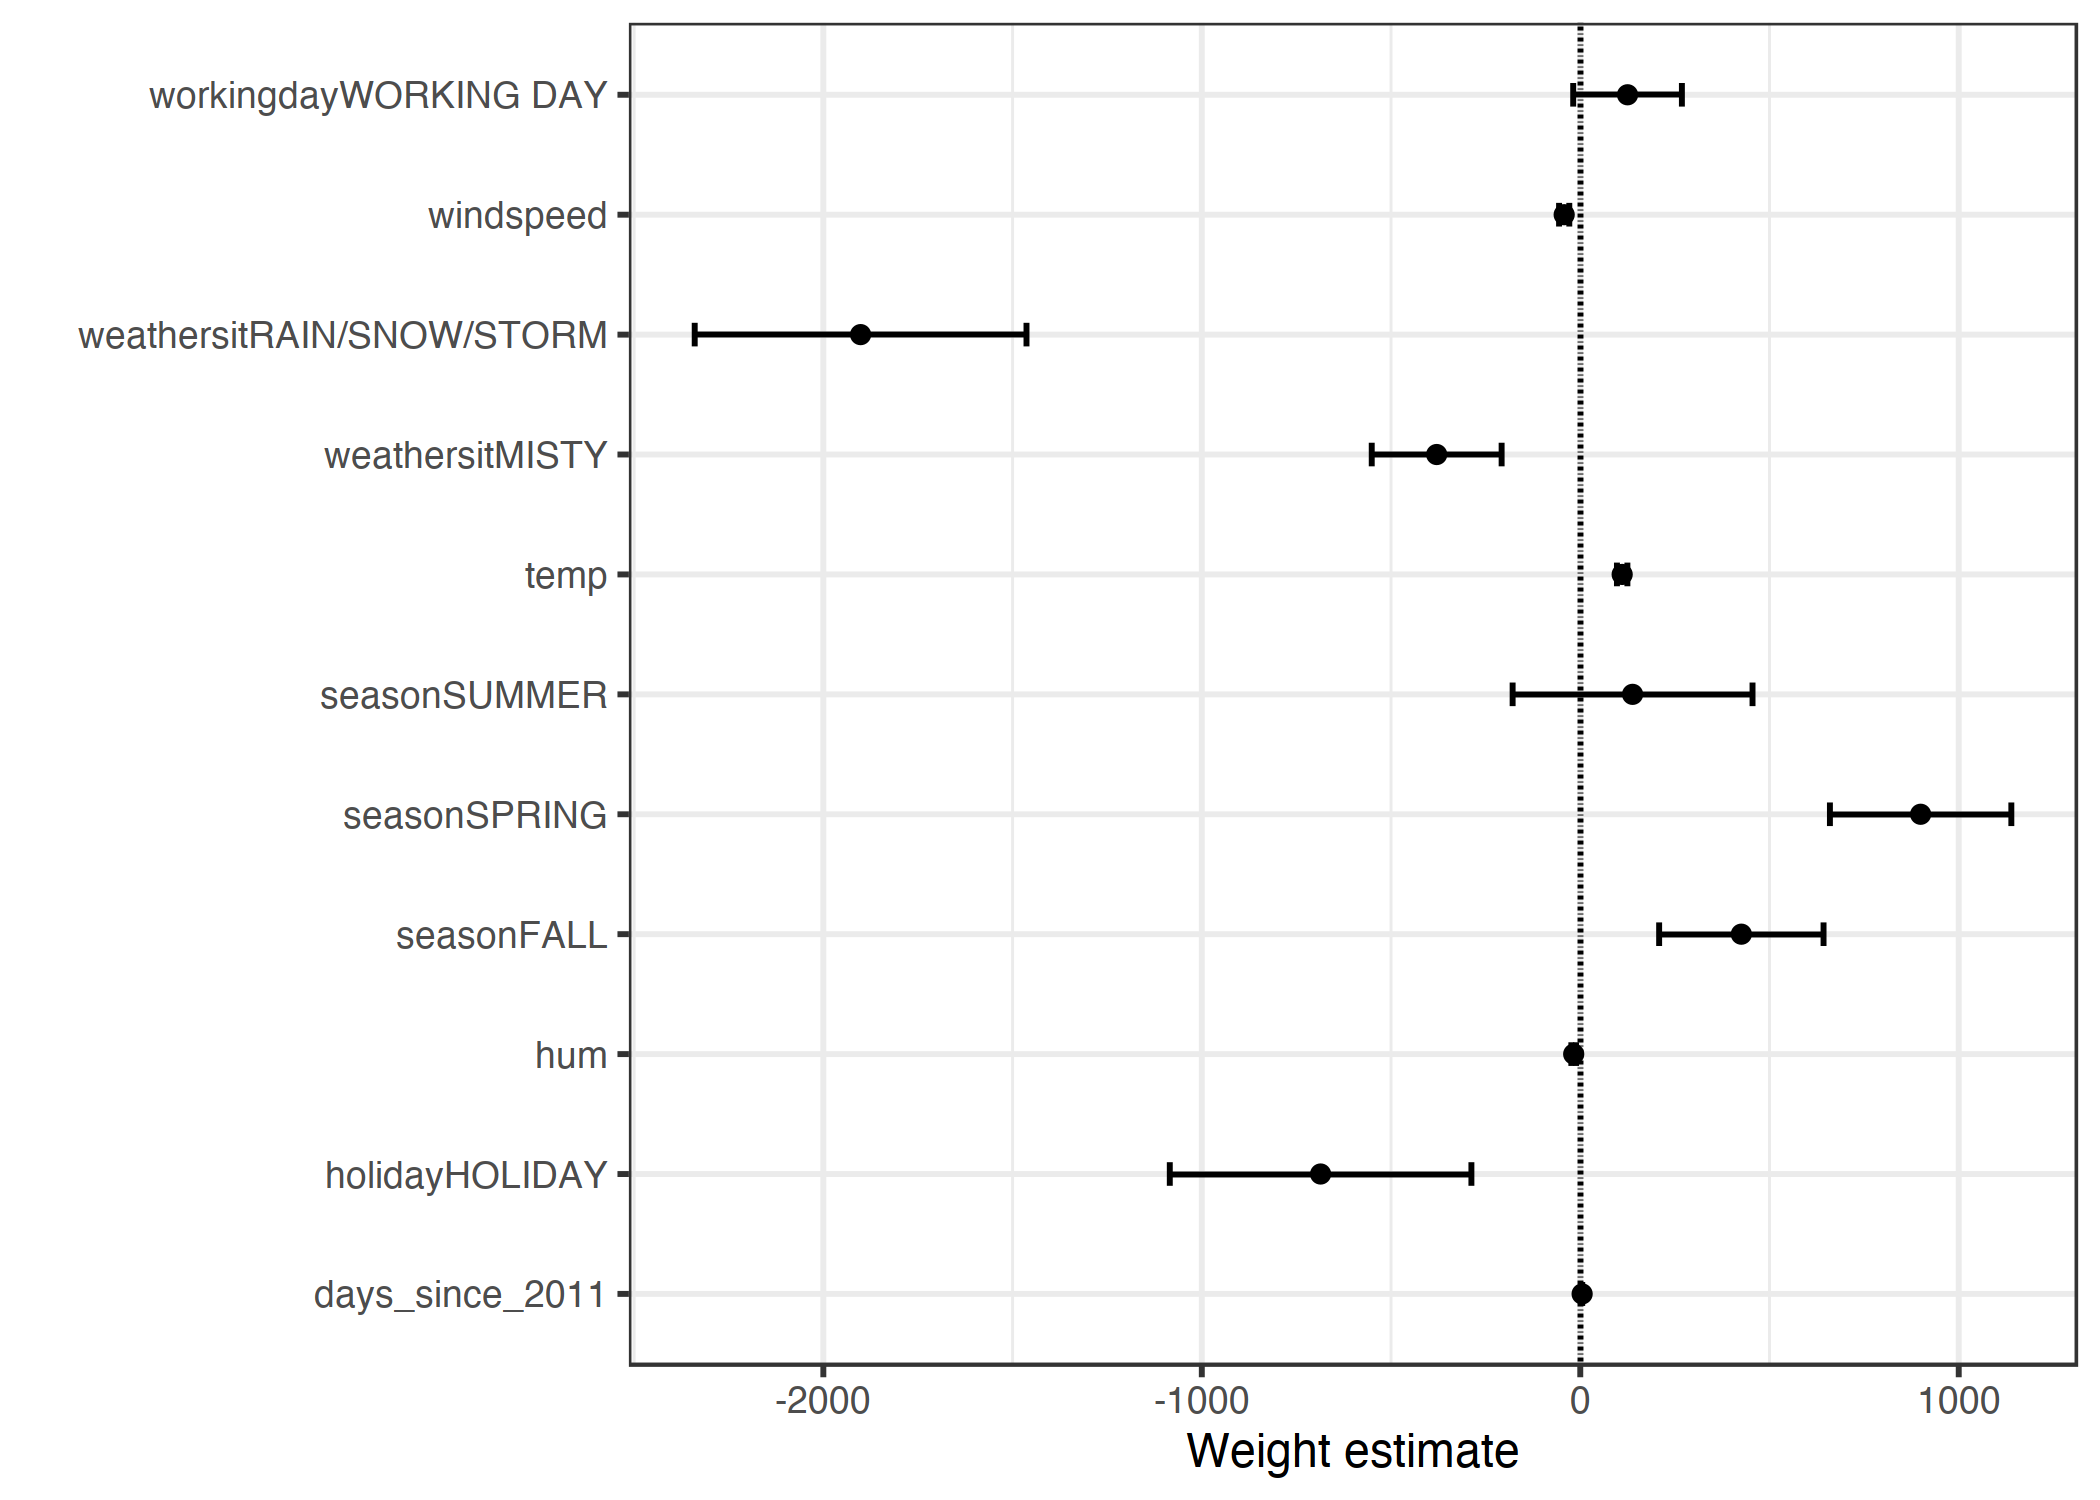
\includegraphics[width=\textwidth]{images/linear-weights-plot-1} 

}

\caption{Weights are displayed as points and the 95\% confidence intervals as lines.}\label{fig:linear-weights-plot}
\end{figure}

The weight plot shows that rainy/snowy/stormy weather has a strong negative effect on the predicted number of bikes.
The weight of the working day feature is close to zero and zero is included in the 95\% interval, which means that the effect is not statistically significant.
Some confidence intervals are very short and the estimates are close to zero, yet the feature effects were statistically significant.
Temperature is one such candidate.
The problem with the weight plot is that the features are measured on different scales.
While for the weather the estimated weight reflects the difference between good and rainy/stormy/snowy weather, for temperature it only reflects an increase of 1 degree Celsius.
You can make the estimated weights more comparable by scaling the features (zero mean and standard deviation of one) before fitting the linear model.

\hypertarget{effect-plot}{%
\subsubsection{Effect Plot}\label{effect-plot}}

The weights of the linear regression model can be more meaningfully analyzed when they are multiplied by the actual feature values.
The weights depend on the scale of the features and will be different if you have a feature that measures e.g.~a person's height and you switch from meter to centimeter.
The weight will change, but the actual effects in your data will not.
It is also important to know the distribution of your feature in the data, because if you have a very low variance, it means that almost all instances have similar contribution from this feature.
The effect plot can help you understand how much the combination of weight and feature contributes to the predictions in your data.
Start by calculating the effects, which is the weight per feature times the feature value of an instance:

\[\text{effect}_{j}^{(i)}=w_{j}x_{j}^{(i)}\]

The effects can be visualized with boxplots.
A box in a boxplot contains the effect range for half of your data (25\% to 75\% effect quantiles).
The vertical line in the box is the median effect, i.e.~50\% of the instances have a lower and the other half a higher effect on the prediction.
The horizontal lines extend to \(\pm1.5\text{IQR}/\sqrt{n}\), with IQR being the inter quartile range (75\% quantile minus 25\% quantile).
The dots are outliers.
The categorical feature effects can be summarized in a single boxplot, compared to the weight plot, where each category has its own row.

\begin{figure}

{\centering \includegraphics[width=\textwidth]{images/linear-effects-1} 

}

\caption{The feature effect plot shows the distribution of effects (= feature value times feature weight) across the data per feature.}\label{fig:linear-effects}
\end{figure}

The largest contributions to the expected number of rented bicycles comes from the temperature feature and the days feature, which captures the trend of bike rentals over time.
The temperature has a broad range of how much it contributes to the prediction.
The day trend feature goes from zero to large positive contributions, because the first day in the dataset (01.01.2011) has a very small trend effect and the estimated weight for this feature is positive (4.93).
This means that the effect increases with each day and is highest for the last day in the dataset (31.12.2012).
Note that for effects with a negative weight, the instances with a positive effect are those that have a negative feature value.
For example, days with a high negative effect of windspeed are the ones with high wind speeds.

\hypertarget{explain-individual-predictions}{%
\subsection{Explain Individual Predictions}\label{explain-individual-predictions}}

How much has each feature of an instance contributed to the prediction?
This can be answered by computing the effects for this instance.
An interpretation of instance-specific effects only makes sense in comparison to the distribution of the effect for each feature.
We want to explain the prediction of the linear model for the 6-th instance from the bicycle dataset.
The instance has the following feature values.

\begin{tabular}{l|l}
\hline
Feature & Value\\
\hline
season & SPRING\\
\hline
yr & 2011\\
\hline
mnth & JAN\\
\hline
holiday & NO HOLIDAY\\
\hline
weekday & THU\\
\hline
workingday & WORKING DAY\\
\hline
weathersit & GOOD\\
\hline
temp & 1.604356\\
\hline
hum & 51.8261\\
\hline
windspeed & 6.000868\\
\hline
cnt & 1606\\
\hline
days\_since\_2011 & 5\\
\hline
\end{tabular}

To obtain the feature effects of this instance, we have to multiply its feature values by the corresponding weights from the linear regression model.
For the value ``WORKING DAY'' of feature ``workingday'', the effect is, 124.9.
For a temperature of 1.6 degrees Celsius, the effect is 177.6.
We add these individual effects as crosses to the effect plot, which shows us the distribution of the effects in the data.
This allows us to compare the individual effects with the distribution of effects in the data.

\begin{figure}

{\centering \includegraphics[width=\textwidth]{images/linear-effects-single-1} 

}

\caption{The effect plot for one instance shows the effect distribution and highlights the effects of the instance of interest.}\label{fig:linear-effects-single}
\end{figure}

If we average the predictions for the training data instances, we get an average of 4504.
In comparison, the prediction of the 6-th instance is small, since only 1571 bicycle rents are predicted.
The effect plot reveals the reason why.
The boxplots show the distributions of the effects for all instances of the dataset, the crosses show the effects for the 6-th instance.
The 6-th instance has a low temperature effect because on this day the temperature was 2 degrees, which is low compared to most other days (and remember that the weight of the temperature feature is positive).
Also, the effect of the trend feature ``days\_since\_2011'' is small compared to the other data instances because this instance is from early 2011 (5 days) and the trend feature also has a positive weight.

\hypertarget{cat-code}{%
\subsection{Encoding of Categorical Features}\label{cat-code}}

There are several ways to encode a categorical feature, and the choice influences the interpretation of the weights.

The standard in linear regression models is treatment coding, which is sufficient in most cases.
Using different encodings boils down to creating different (design) matrices from a single column with the categorical feature.
This section presents three different encodings, but there are many more.
The example used has six instances and a categorical feature with three categories.
For the first two instances, the feature takes category A;
for instances three and four, category B;
and for the last two instances, category C.

\textbf{Treatment coding}

In treatment coding, the weight per category is the estimated difference in the prediction between the corresponding category and the reference category.
The intercept of the linear model is the mean of the reference category (when all other features remain the same).
The first column of the design matrix is the intercept, which is always 1.
Column two indicates whether instance i is in category B, column three indicates whether it is in category C.
There is no need for a column for category A, because then the linear equation would be overspecified and no unique solution for the weights can be found.
It is sufficient to know that an instance is neither in category B or C.

Feature matrix: \[\begin{pmatrix}1&0&0\\1&0&0\\1&1&0\\1&1&0\\1&0&1\\1&0&1\\\end{pmatrix}\]

\textbf{Effect coding}

The weight per category is the estimated y-difference from the corresponding category to the overall mean (given all other features are zero or the reference category).
The first column is used to estimate the intercept.
The weight \(\beta_{0}\) associated with the intercept represents the overall mean and \(\beta_{1}\), the weight for column two, is the difference between the overall mean and category B.
The total effect of category B is \(\beta_{0}+\beta_{1}\).
The interpretation for category C is equivalent.
For the reference category A, \(-(\beta_{1}+\beta_{2})\) is the difference to the overall mean and \(\beta_{0}-(\beta_{1}+\beta_{2})\) the overall effect.

Feature matrix: \[\begin{pmatrix}1&-1&-1\\1&-1&-1\\1&1&0\\1&1&0\\1&0&1\\1&0&1\\\end{pmatrix}\]

\textbf{Dummy coding}

The \(\beta\) per category is the estimated mean value of y for each category (given all other feature values are zero or the reference category).
Note that the intercept has been omitted here so that a unique solution can be found for the linear model weights.
Another way to mitigate this multicollinearity problem is to leave out one of the categories.

Feature matrix: \[\begin{pmatrix}1&0&0\\1&0&0\\0&1&0\\0&1&0\\0&0&1\\0&0&1\\\end{pmatrix}\]

If you want to dive a little deeper into the different encodings of categorical features, checkout \href{http://stats.idre.ucla.edu/r/library/r-library-contrast-coding-systems-for-categorical-variables/}{this overview webpage} and
\href{http://heidiseibold.github.io/page7/}{this blog post}.

\hypertarget{do-linear-models-create-good-explanations}{%
\subsection{Do Linear Models Create Good Explanations?}\label{do-linear-models-create-good-explanations}}

Judging by the attributes that constitute a good explanation, as presented \protect\hyperlink{good-explanation}{in the Human-Friendly Explanations chapter}, linear models do not create the best explanations.
They are contrastive, but the reference instance is a data point where all numerical features are zero and the categorical features are at their reference categories.
This is usually an artificial, meaningless instance that is unlikely to occur in your data or reality.
There is an exception:
If all numerical features are mean centered (feature minus mean of feature) and all categorical features are effect coded, the reference instance is the data point where all the features take on the mean feature value.
This might also be a non-existent data point, but it might at least be more likely or more meaningful.
In this case, the weights times the feature values (feature effects) explain the contribution to the predicted outcome contrastive to the ``mean-instance''.
Another aspect of a good explanation is selectivity, which can be achieved in linear models by using less features or by training sparse linear models.
But by default, linear models do not create selective explanations.
Linear models create truthful explanations, as long as the linear equation is an appropriate model for the relationship between features and outcome.
The more non-linearities and interactions there are, the less accurate the linear model will be and the less truthful the explanations become.
Linearity makes the explanations more general and simpler.
The linear nature of the model, I believe, is the main factor why people use linear models for explaining relationships.

\hypertarget{sparse-linear}{%
\subsection{Sparse Linear Models}\label{sparse-linear}}

The examples of the linear models that I have chosen all look nice and neat, do they not?
But in reality you might not have just a handful of features, but hundreds or thousands.
And your linear regression models?
Interpretability goes downhill.
You might even find yourself in a situation where there are more features than instances, and you cannot fit a standard linear model at all.
The good news is that there are ways to introduce sparsity (= few features) into linear models.

\hypertarget{lasso}{%
\subsubsection{Lasso}\label{lasso}}

Lasso is an automatic and convenient way to introduce sparsity into the linear regression model.
Lasso stands for ``least absolute shrinkage and selection operator'' and, when applied in a linear regression model, performs feature selection and regularization of the selected feature weights.
Let us consider the minimization problem that the weights optimize:

\[min_{\boldsymbol{\beta}}\left(\frac{1}{n}\sum_{i=1}^n(y^{(i)}-x_i^T\boldsymbol{\beta})^2\right)\]

Lasso adds a term to this optimization problem.

\[min_{\boldsymbol{\beta}}\left(\frac{1}{n}\sum_{i=1}^n(y^{(i)}-x_{i}^T\boldsymbol{\beta})^2+\lambda||\boldsymbol{\beta}||_1\right)\]

The term \(||\boldsymbol{\beta}||_1\), the L1-norm of the feature vector, leads to a penalization of large weights.
Since the L1-norm is used, many of the weights receive an estimate of 0 and the others are shrunk.
The parameter lambda (\(\lambda\)) controls the strength of the regularizing effect and is usually tuned by cross-validation.
Especially when lambda is large, many weights become 0.
The feature weights can be visualized as a function of the penalty term lambda.
Each feature weight is represented by a curve in the following figure.

\begin{figure}

{\centering \includegraphics[width=\textwidth]{images/lasso-path-1} 

}

\caption{With increasing penalty of the weights, fewer and fewer features receive a non-zero weight estimate. These curves are also called regularization paths. The number above the plot is the number of non-zero weights.}\label{fig:lasso-path}
\end{figure}

What value should we choose for lambda?
If you see the penalization term as a tuning parameter, then you can find the lambda that minimizes the model error with cross-validation.
You can also consider lambda as a parameter to control the interpretability of the model.
The larger the penalization, the fewer features are present in the model (because their weights are zero) and the better the model can be interpreted.

\textbf{Example with Lasso}

We will predict bicycle rentals using Lasso.
We set the number of features we want to have in the model beforehand.
Let us first set the number to 2 features:

\begin{tabular}{l|r}
\hline
  & Weight\\
\hline
seasonSPRING & 0.00\\
\hline
seasonSUMMER & 0.00\\
\hline
seasonFALL & 0.00\\
\hline
seasonWINTER & 0.00\\
\hline
holidayHOLIDAY & 0.00\\
\hline
workingdayWORKING DAY & 0.00\\
\hline
weathersitMISTY & 0.00\\
\hline
weathersitRAIN/SNOW/STORM & 0.00\\
\hline
temp & 52.33\\
\hline
hum & 0.00\\
\hline
windspeed & 0.00\\
\hline
days\_since\_2011 & 2.15\\
\hline
\end{tabular}

The first two features with non-zero weights in the Lasso path are temperature (``temp'') and the time trend (``days\_since\_2011'').

Now, let us select 5 features:

\begin{tabular}{l|r}
\hline
  & Weight\\
\hline
seasonSPRING & -389.99\\
\hline
seasonSUMMER & 0.00\\
\hline
seasonFALL & 0.00\\
\hline
seasonWINTER & 0.00\\
\hline
holidayHOLIDAY & 0.00\\
\hline
workingdayWORKING DAY & 0.00\\
\hline
weathersitMISTY & 0.00\\
\hline
weathersitRAIN/SNOW/STORM & -862.27\\
\hline
temp & 85.58\\
\hline
hum & -3.04\\
\hline
windspeed & 0.00\\
\hline
days\_since\_2011 & 3.82\\
\hline
\end{tabular}

Note that the weights for ``temp'' and ``days\_since\_2011'' differ from the model with two features.
The reason for this is that by decreasing lambda even features that are already ``in'' the model are penalized less and may get a larger absolute weight.
The interpretation of the Lasso weights corresponds to the interpretation of the weights in the linear regression model.
You only need to pay attention to whether the features are standardized or not, because this affects the weights.
In this example, the features were standardized by the software, but the weights were automatically transformed back for us to match the original feature scales.

\textbf{Other methods for sparsity in linear models}

A wide spectrum of methods can be used to reduce the number of features in a linear model.

Pre-processing methods:

\begin{itemize}
\tightlist
\item
  Manually selected features:
  You can always use expert knowledge to select or discard some features.
  The big drawback is that it cannot be automated and you need to have access to someone who understands the data.
\item
  Univariate selection:
  An example is the correlation coefficient.
  You only consider features that exceed a certain threshold of correlation between the feature and the target.
  The disadvantage is that it only considers the features individually.
  Some features might not show a correlation until the linear model has accounted for some other features.
  Those ones you will miss with univariate selection methods.
\end{itemize}

Step-wise methods:

\begin{itemize}
\tightlist
\item
  Forward selection:
  Fit the linear model with one feature.
  Do this with each feature.
  Select the model that works best (e.g.~highest R-squared).
  Now again, for the remaining features, fit different versions of your model by adding each feature to your current best model.
  Select the one that performs best.
  Continue until some criterion is reached, such as the maximum number of features in the model.
\item
  Backward selection:
  Similar to forward selection.
  But instead of adding features, start with the model that contains all features and try out which feature you have to remove to get the highest performance increase.
  Repeat this until some stopping criterion is reached.
\end{itemize}

I recommend using Lasso, because it can be automated, considers all features simultaneously, and can be controlled via lambda.
It also works for the \protect\hyperlink{logistic}{logistic regression model} for classification.

\hypertarget{advantages}{%
\subsection{Advantages}\label{advantages}}

The modeling of the predictions as a \textbf{weighted sum} makes it transparent how predictions are produced.
And with Lasso we can ensure that the number of features used remains small.

Many people use linear regression models.
This means that in many places it is \textbf{accepted} for predictive modeling and doing inference.
There is a \textbf{high level of collective experience and expertise}, including teaching materials on linear regression models and software implementations.
Linear regression can be found in R, Python, Java, Julia, Scala, Javascript, \ldots{}

Mathematically, it is straightforward to estimate the weights and you have a \textbf{guarantee to find optimal weights} (given all assumptions of the linear regression model are met by the data).

Together with the weights you get confidence intervals, tests, and solid statistical theory.
There are also many extensions of the linear regression model (see \protect\hyperlink{extend-lm}{chapter on GLM, GAM and more}).

\hypertarget{disadvantages}{%
\subsection{Disadvantages}\label{disadvantages}}

Linear regression models can only represent linear relationships, i.e.~a weighted sum of the input features.
Each \textbf{nonlinearity or interaction has to be hand-crafted} and explicitly given to the model as an input feature.

Linear models are also often \textbf{not that good regarding predictive performance}, because the relationships that can be learned are so restricted and usually oversimplify how complex reality is.

The interpretation of a weight \textbf{can be unintuitive} because it depends on all other features.
A feature with high positive correlation with the outcome y and another feature might get a negative weight in the linear model, because, given the other correlated feature, it is negatively correlated with y in the high-dimensional space.
Completely correlated features make it even impossible to find a unique solution for the linear equation.
An example:
You have a model to predict the value of a house and have features like number of rooms and size of the house.
House size and number of rooms are highly correlated: the bigger a house is, the more rooms it has.
If you take both features into a linear model, it might happen, that the size of the house is the better predictor and gets a large positive weight.
The number of rooms might end up getting a negative weight, because, given that a house has the same size, increasing the number of rooms could make it less valuable or the linear equation becomes less stable, when the correlation is too strong.

\newpage

\hypertarget{logistic}{%
\section{Logistic Regression}\label{logistic}}

Logistic regression models the probabilities for classification problems with two possible outcomes.
It's an extension of the linear regression model for classification problems.

\hypertarget{what-is-wrong-with-linear-regression-for-classification}{%
\subsection{What is Wrong with Linear Regression for Classification?}\label{what-is-wrong-with-linear-regression-for-classification}}

The linear regression model can work well for regression, but fails for classification.
Why is that?
In case of two classes, you could label one of the classes with 0 and the other with 1 and use linear regression.
Technically it works and most linear model programs will spit out weights for you.
But there are a few problems with this approach:

A linear model does not output probabilities, but it treats the classes as numbers (0 and 1) and fits the best hyperplane (for a single feature, it is a line) that minimizes the distances between the points and the hyperplane.
So it simply interpolates between the points, and you cannot interpret it as probabilities.

A linear model also extrapolates and gives you values below zero and above one.
This is a good sign that there might be a smarter approach to classification.

Since the predicted outcome is not a probability, but a linear interpolation between points, there is no meaningful threshold at which you can distinguish one class from the other.
A good illustration of this issue has been given on \href{https://stats.stackexchange.com/questions/22381/why-not-approach-classification-through-regression}{Stackoverflow}.

Linear models do not extend to classification problems with multiple classes.
You would have to start labeling the next class with 2, then 3, and so on.
The classes might not have any meaningful order, but the linear model would force a weird structure on the relationship between the features and your class predictions.
The higher the value of a feature with a positive weight, the more it contributes to the prediction of a class with a higher number, even if classes that happen to get a similar number are not closer than other classes.

\begin{figure}

{\centering \includegraphics[width=\textwidth]{images/linear-class-threshold-1} 

}

\caption{A linear model classifies tumors as malignant (1) or benign (0) given their size. The lines show the prediction of the linear model. For the data on the left, we can use 0.5 as classification threshold. After introducing a few more malignant tumor cases, the regression line shifts and a threshold of 0.5 no longer separates the classes. Points are slightly jittered to reduce over-plotting. }\label{fig:linear-class-threshold}
\end{figure}

\hypertarget{theory}{%
\subsection{Theory}\label{theory}}

A solution for classification is logistic regression.
Instead of fitting a straight line or hyperplane, the logistic regression model uses the logistic function to squeeze the output of a linear equation between 0 and 1.
The logistic function is defined as:

\[\text{logistic}(\eta)=\frac{1}{1+exp(-\eta)}\]

And it looks like this:

\begin{figure}

{\centering \includegraphics[width=\textwidth]{images/logistic-function-1} 

}

\caption{The logistic function. It outputs numbers between 0 and 1. At input 0, it outputs 0.5.}\label{fig:logistic-function}
\end{figure}

The step from linear regression to logistic regression is kind of straightforward.
In the linear regression model, we have modelled the relationship between outcome and features with a linear equation:

\[\hat{y}^{(i)}=\beta_{0}+\beta_{1}x^{(i)}_{1}+\ldots+\beta_{p}x^{(i)}_{p}\]

For classification, we prefer probabilities between 0 and 1, so we wrap the right side of the equation into the logistic function.
This forces the output to assume only values between 0 and 1.

\[P(y^{(i)}=1)=\frac{1}{1+exp(-(\beta_{0}+\beta_{1}x^{(i)}_{1}+\ldots+\beta_{p}x^{(i)}_{p}))}\]

Let us revisit the tumor size example again.
But instead of the linear regression model, we use the logistic regression model:

\begin{figure}

{\centering \includegraphics[width=\textwidth]{images/logistic-class-threshold-1} 

}

\caption{The logistic regression model finds the correct decision boundary between malignant and benign depending on tumor size. The line is the logistic function shifted and squeezed to fit the data.}\label{fig:logistic-class-threshold}
\end{figure}

Classification works better with logistic regression and we can use 0.5 as a threshold in both cases. The inclusion of additional points does not really affect the estimated curve.

\hypertarget{interpretation-1}{%
\subsection{Interpretation}\label{interpretation-1}}

The interpretation of the weights in logistic regression differs from the interpretation of the weights in linear regression, since the outcome in logistic regression is a probability between 0 and 1.
The weights do not influence the probability linearly any longer.
The weighted sum is transformed by the logistic function to a probability.
Therefore we need to reformulate the equation for the interpretation so that only the linear term is on the right side of the formula.

\[log\left(\frac{P(y=1)}{1-P(y=1)}\right)=log\left(\frac{P(y=1)}{P(y=0)}\right)=\beta_{0}+\beta_{1}x_{1}+\ldots+\beta_{p}x_{p}\]

We call the term in the log() function ``odds'' (probability of event divided by probability of no event) and wrapped in the logarithm it is called log odds.

This formula shows that the logistic regression model is a linear model for the log odds.
Great!
That does not sound helpful!
With a little shuffling of the terms, you can figure out how the prediction changes when one of the features \(x_j\) is changed by 1 unit.
To do this, we can first apply the exp() function to both sides of the equation:

\[\frac{P(y=1)}{1-P(y=1)}=odds=exp\left(\beta_{0}+\beta_{1}x_{1}+\ldots+\beta_{p}x_{p}\right)\]

Then we compare what happens when we increase one of the feature values by 1.
But instead of looking at the difference, we look at the ratio of the two predictions:

\[\frac{odds_{x_j+1}}{odds}=\frac{exp\left(\beta_{0}+\beta_{1}x_{1}+\ldots+\beta_{j}(x_{j}+1)+\ldots+\beta_{p}x_{p}\right)}{exp\left(\beta_{0}+\beta_{1}x_{1}+\ldots+\beta_{j}x_{j}+\ldots+\beta_{p}x_{p}\right)}\]

We apply the following rule:

\[\frac{exp(a)}{exp(b)}=exp(a-b)\]

And we remove many terms:

\[\frac{odds_{x_j+1}}{odds}=exp\left(\beta_{j}(x_{j}+1)-\beta_{j}x_{j}\right)=exp\left(\beta_j\right)\]

In the end, we have something as simple as exp() of a feature weight.
A change in a feature by one unit changes the odds ratio (multiplicative) by a factor of \(\exp(\beta_j)\).
We could also interpret it this way:
A change in \(x_j\) by one unit increases the log odds ratio by the value of the corresponding weight.
Most people interpret the odds ratio because thinking about the log() of something is known to be hard on the brain.
Interpreting the odds ratio already requires some getting used to.
For example, if you have odds of 2, it means that the probability for y=1 is twice as high as y=0.
If you have a weight (= log odds ratio) of 0.7, then increasing the respective feature by one unit multiplies the odds by exp(0.7) (approximately 2) and the odds change to 4.
But usually you do not deal with the odds and interpret the weights only as the odds ratios.
Because for actually calculating the odds you would need to set a value for each feature, which only makes sense if you want to look at one specific instance of your dataset.

These are the interpretations for the logistic regression model with different feature types:

\begin{itemize}
\tightlist
\item
  Numerical feature:
  If you increase the value of feature \(x_{j}\) by one unit, the estimated odds change by a factor of \(\exp(\beta_{j})\)
\item
  Binary categorical feature:
  One of the two values of the feature is the reference category (in some languages, the one encoded in 0).
  Changing the feature \(x_{j}\) from the reference category to the other category changes the estimated odds by a factor of \(\exp(\beta_{j})\).
\item
  Categorical feature with more than two categories:
  One solution to deal with multiple categories is one-hot-encoding, meaning that each category has its own column.
  You only need L-1 columns for a categorical feature with L categories, otherwise it is over-parameterized.
  The L-th category is then the reference category.
  You can use any other encoding that can be used in linear regression.
  The interpretation for each category then is equivalent to the interpretation of binary features.
\item
  Intercept \(\beta_{0}\):
  When all numerical features are zero and the categorical features are at the reference category, the estimated odds are \(\exp(\beta_{0})\).
  The interpretation of the intercept weight is usually not relevant.
\end{itemize}

\hypertarget{example-1}{%
\subsection{Example}\label{example-1}}

We use the logistic regression model to predict \protect\hyperlink{cervical}{cervical cancer} based on some risk factors.
The following table shows the estimate weights, the associated odds ratios, and the standard error of the estimates.

\begin{table}

\caption{\label{tab:logistic-example}The results of fitting a logistic regression model on the cervical cancer dataset. Shown are the features used in the model, their estimated weights and corresponding odds ratios, and the standard errors of the estimated weights.}
\centering
\begin{tabular}[t]{l|r|r|r}
\hline
  & Weight & Odds ratio & Std. Error\\
\hline
Intercept & -2.91 & 0.05 & 0.32\\
\hline
Hormonal contraceptives y/n & -0.12 & 0.89 & 0.30\\
\hline
Smokes y/n & 0.26 & 1.30 & 0.37\\
\hline
Num. of pregnancies & 0.04 & 1.04 & 0.10\\
\hline
Num. of diagnosed STDs & 0.82 & 2.27 & 0.33\\
\hline
Intrauterine device y/n & 0.62 & 1.86 & 0.40\\
\hline
\end{tabular}
\end{table}

Interpretation of a numerical feature (``Num. of diagnosed STDs''):
An increase in the number of diagnosed STDs (sexually transmitted diseases) changes (increases) the odds of cancer vs.~no cancer by a factor of 2.27, when all other features remain the same.
Keep in mind that correlation does not imply causation.

Interpretation of a categorical feature (``Hormonal contraceptives y/n''):
For women using hormonal contraceptives, the odds for cancer vs.~no cancer are by a factor of 0.89 lower, compared to women without hormonal contraceptives, given all other features stay the same.

Like in the linear model, the interpretations always come with the clause that `all other features stay the same'.

\hypertarget{advantages-and-disadvantages}{%
\subsection{Advantages and Disadvantages}\label{advantages-and-disadvantages}}

Many of the pros and cons of the \protect\hyperlink{limo}{linear regression model} also apply to the logistic regression model.
Logistic regression has been widely used by many different people, but it struggles with its restrictive expressiveness (e.g.~interactions must be added manually) and other models may have better predictive performance.

Another disadvantage of the logistic regression model is that the interpretation is more difficult because the interpretation of the weights is multiplicative and not additive.

Logistic regression can suffer from \textbf{complete separation}.
If there is a feature that would perfectly separate the two classes, the logistic regression model can no longer be trained.
This is because the weight for that feature would not converge, because the optimal weight would be infinite.
This is really a bit unfortunate, because such a feature is really useful.
But you do not need machine learning if you have a simple rule that separates both classes.
The problem of complete separation can be solved by introducing penalization of the weights or defining a prior probability distribution of weights.

On the good side, the logistic regression model is not only a classification model, but also gives you probabilities.
This is a big advantage over models that can only provide the final classification.
Knowing that an instance has a 99\% probability for a class compared to 51\% makes a big difference.

Logistic regression can also be extended from binary classification to multi-class classification.
Then it is called Multinomial Regression.

\hypertarget{software}{%
\subsection{Software}\label{software}}

I used the \texttt{glm} function in R for all examples.
You can find logistic regression in any programming language that can be used for performing data analysis, such as Python, Java, Stata, Matlab, \ldots{}

\newpage

\hypertarget{extend-lm}{%
\section{GLM, GAM and more}\label{extend-lm}}

The biggest strength but also the biggest weakness of the \protect\hyperlink{limo}{linear regression model} is that the prediction is modeled as a weighted sum of the features.
In addition, the linear model comes with many other assumptions.
The bad news is (well, not really news) that all those assumptions are often violated in reality:
The outcome given the features might have a non-Gaussian distribution, the features might interact and the relationship between the features and the outcome might be nonlinear.
The good news is that the statistics community has developed a variety of modifications that transform the linear regression model from a simple blade into a Swiss knife.

This chapter is definitely not your definite guide to extending linear models.
Rather, it serves as an overview of extensions such as Generalized Linear Models (GLMs) and Generalized Additive Models (GAMs) and gives you a little intuition.
After reading, you should have a solid overview of how to extend linear models.
If you want to learn more about the linear regression model first, I suggest you read the \protect\hyperlink{limo}{chapter on linear regression models}, if you have not already.

Let us remember the formula of a linear regression model:

\[y=\beta_{0}+\beta_{1}x_{1}+\ldots+\beta_{p}x_{p}+\epsilon\]

The linear regression model assumes that the outcome y of an instance can be expressed by a weighted sum of its p features with an individual error \(\epsilon\) that follows a Gaussian distribution.
By forcing the data into this corset of a formula, we obtain a lot of model interpretability.
The feature effects are additive, meaning no interactions, and the relationship is linear, meaning an increase of a feature by one unit can be directly translated into an increase/decrease of the predicted outcome.
The linear model allows us to compress the relationship between a feature and the expected outcome into a single number, namely the estimated weight.

But a simple weighted sum is too restrictive for many real world prediction problems.
In this chapter we will learn about three problems of the classical linear regression model and how to solve them.
There are many more problems with possibly violated assumptions, but we will focus on the three shown in the following figure:

\begin{figure}

{\centering \includegraphics[width=\textwidth]{images/three-lm-problems-1} 

}

\caption{Three assumptions of the linear model (left side): Gaussian distribution of the outcome given the features, additivity (= no interactions) and linear relationship. Reality usually does not adhere to those assumptions (right side): Outcomes might have non-Gaussian distributions, features might interact and the relationship might be nonlinear.}\label{fig:three-lm-problems}
\end{figure}

There is a solution to all these problems:

\textbf{Problem}: The target outcome y given the features does not follow a Gaussian distribution.\\
\textbf{Example}: Suppose I want to predict how many minutes I will ride my bike on a given day.
As features I have the type of day, the weather and so on.
If I use a linear model, it could predict negative minutes because it assumes a Gaussian distribution which does not stop at 0 minutes.
Also if I want to predict probabilities with a linear model, I can get probabilities that are negative or greater than 1.\\
\textbf{Solution}: \protect\hyperlink{glm}{Generalized Linear Models (GLMs)}.

\textbf{Problem}: The features interact.\\
\textbf{Example}: On average, light rain has a slight negative effect on my desire to go cycling.
But in summer, during rush hour, I welcome rain, because then all the fair-weather cyclists stay at home and I have the bicycle paths for myself!
This is an interaction between time and weather that cannot be captured by a purely additive model.\\
\textbf{Solution}: \protect\hyperlink{lm-interact}{Adding interactions manually}.

\textbf{Problem}: The true relationship between the features and y is not linear.\\
\textbf{Example}: Between 0 and 25 degrees Celsius, the influence of the temperature on my desire to ride a bike could be linear, which means that an increase from 0 to 1 degree causes the same increase in cycling desire as an increase from 20 to 21.
But at higher temperatures my motivation to cycle levels off and even decreases - I do not like to bike when it is too hot.\\
\textbf{Solutions}: \protect\hyperlink{gam}{Generalized Additive Models (GAMs); transformation of features}.

The solutions to these three problems are presented in this chapter.
Many further extensions of the linear model are omitted.
If I attempted to cover everything here, the chapter would quickly turn into a book within a book about a topic that is already covered in many other books.
But since you are already here, I have made a little problem plus solution overview for linear model extensions, which you can find at the \protect\hyperlink{more-lm-extension}{end of the chapter}.
The name of the solution is meant to serve as a starting point for a search.

\hypertarget{glm}{%
\subsection{Non-Gaussian Outcomes - GLMs}\label{glm}}

The linear regression model assumes that the outcome given the input features follows a Gaussian distribution.
This assumption excludes many cases:
The outcome can also be a category (cancer vs.~healthy), a count (number of children), the time to the occurrence of an event (time to failure of a machine) or a very skewed outcome with a few very high values (household income).
The linear regression model can be extended to model all these types of outcomes.
This extension is called \textbf{Generalized Linear Models} or \textbf{GLMs} for short.
Throughout this chapter, I will use the name GLM for both the general framework and for particular models from that framework.
The core concept of any GLM is:
Keep the weighted sum of the features, but allow non-Gaussian outcome distributions and connect the expected mean of this distribution and the weighted sum through a possibly nonlinear function.
For example, the logistic regression model assumes a Bernoulli distribution for the outcome and links the expected mean and the weighted sum using the logistic function.

The GLM mathematically links the weighted sum of the features with the mean value of the assumed distribution using the link function g, which can be chosen flexibly depending on the type of outcome.

\[g(E_Y(y|x))=\beta_0+\beta_1{}x_{1}+\ldots{}\beta_p{}x_{p}\]

GLMs consist of three components:
The link function g, the weighted sum \(X^T\beta\) (sometimes called linear predictor) and a probability distribution from the exponential family that defines \(E_Y\).

The exponential family is a set of distributions that can be written with the same (parameterized) formula that includes an exponent, the mean and variance of the distribution and some other parameters.
I will not go into the mathematical details because this is a very big universe of its own that I do not want to enter.
Wikipedia has a neat \href{https://en.wikipedia.org/wiki/Exponential_family\#Table_of_distributions}{list of distributions from the exponential family}.
Any distribution from this list can be chosen for your GLM.
Based on the type of the outcome you want to predict, choose a suitable distribution.
Is the outcome a count of something (e.g.~number of children living in a household)?
Then the Poisson distribution could be a good choice.
Is the outcome always positive (e.g.~time between two events)?
Then the exponential distribution could be a good choice.

Let us consider the classic linear model as a special case of a GLM.
The link function for the Gaussian distribution in the classic linear model is simply the identity function.
The Gaussian distribution is parameterized by the mean and the variance parameters.
The mean describes the value that we expect on average and the variance describes how much the values vary around this mean.
In the linear model, the link function links the weighted sum of the features to the mean of the Gaussian distribution.

Under the GLM framework, this concept generalizes to any distribution (from the exponential family) and arbitrary link functions.
If y is a count of something, such as the number of coffees someone drinks on a certain day, we could model it with a GLM with a Poisson distribution and the natural logarithm as the link function:

\[ln(E_Y(y|x))=x^{T}\beta\]

The logistic regression model is also a GLM that assumes a Bernoulli distribution and uses the logit function as the link function.
The mean of the binomial distribution used in logistic regression is the probability that y is 1.

\[x^{T}\beta=ln\left(\frac{E_Y(y|x)}{1-E_Y(y|x)}\right)=ln\left(\frac{P(y=1|x)}{1-P(y=1|x)}\right)\]

And if we solve this equation to have P(y=1) on one side, we get the logistic regression formula:

\[P(y=1)=\frac{1}{1+exp(-x^{T}\beta)}\]

Each distribution from the exponential family has a canonical link function that can be derived mathematically from the distribution.
The GLM framework makes it possible to choose the link function independently of the distribution.
How to choose the right link function?
There is no perfect recipe.
You take into account knowledge about the distribution of your target, but also theoretical considerations and how well the model fits your actual data.
For some distributions the canonical link function can lead to values that are invalid for that distribution.
In the case of the exponential distribution, the canonical link function is the negative inverse, which can lead to negative predictions that are outside the domain of the exponential distribution.
Since you can choose any link function, the simple solution is to choose another function that respects the domain of the distribution.

\textbf{Examples}

I have simulated a dataset on coffee drinking behavior to highlight the need for GLMs.
Suppose you have collected data about your daily coffee drinking behavior.
If you do not like coffee, pretend it is about tea.
Along with number of cups, you record your current stress level on a scale of 1 to 10, how well you slept the night before on a scale of 1 to 10 and whether you had to work on that day.
The goal is to predict the number of coffees given the features stress, sleep and work.
I simulated data for 200 days.
Stress and sleep were drawn uniformly between 1 and 10 and work yes/no was drawn with a 50/50 chance (what a life!).
For each day, the number of coffees was then drawn from a Poisson distribution, modelling the intensity \(\lambda\) (which is also the expected value of the Poisson distribution) as a function of the features sleep, stress and work.
You can guess where this story will lead:
\emph{``Hey, let us model this data with a linear model \ldots{} Oh it does not work \ldots{} Let us try a GLM with Poisson distribution \ldots{} SURPRISE! Now it works!''.}
I hope I did not spoil the story too much for you.

Let us look at the distribution of the target variable, the number of coffees on a given day:

\begin{figure}

{\centering \includegraphics[width=\textwidth]{images/poisson-data-1} 

}

\caption{Simulated distribution of number of daily coffees for 200 days.}\label{fig:poisson-data}
\end{figure}

On 76 of the 200 days you had no coffee at all and on the most extreme day you had 7.
Let us naively use a linear model to predict the number of coffees using sleep level, stress level and work yes/no as features.
What can go wrong when we falsely assume a Gaussian distribution?
A wrong assumption can invalidate the estimates, especially the confidence intervals of the weights.
A more obvious problem is that the predictions do not match the ``allowed'' domain of the true outcome, as the following figure shows.

\begin{figure}

{\centering \includegraphics[width=\textwidth]{images/failing-linear-model-1} 

}

\caption{Predicted number of coffees dependent on stress, sleep and work. The linear model predicts negative values.}\label{fig:failing-linear-model}
\end{figure}

The linear model does not make sense, because it predicts negative number of coffees.
This problem can be solved with Generalized Linear Models (GLMs).
We can change the link function and the assumed distribution.
One possibility is to keep the Gaussian distribution and use a link function that always leads to positive predictions such as the log-link (the inverse is the exp-function) instead of the identity function.
Even better:
We choose a distribution that corresponds to the data generating process and an appropriate link function.
Since the outcome is a count, the Poisson distribution is a natural choice, along with the logarithm as link function.
In this case, the data was even generated with the Poisson distribution, so the Poisson GLM is the perfect choice.
The fitted Poisson GLM leads to the following distribution of predicted values:

\begin{figure}

{\centering \includegraphics[width=\textwidth]{images/linear-model-positive-1} 

}

\caption{Predicted number of coffees dependent on stress, sleep and work. The GLM with Poisson assumption and log link is an appropriate model for this dataset.}\label{fig:linear-model-positive}
\end{figure}

No negative amounts of coffees, looks much better now.

\textbf{Interpretation of GLM weights}

The assumed distribution together with the link function determines how the estimated feature weights are interpreted.
In the coffee count example, I used a GLM with Poisson distribution and log link, which implies the following relationship between the expected outcome and the features stress (str), sleep (slp) and work (wrk).

\[ln(E(\text{coffee}|\text{str},\text{slp},\text{wrk}))=\beta_0+\beta_{\text{str}}x_{\text{str}}+\beta_{\text{slp}}x_{\text{slp}}+\beta_{\text{wrk}}x_{\text{wrk}}\]

To interpret the weights we invert the link function so that we can interpret the effect of the features on the expected outcome and not on the logarithm of the expected outcome.

\[E(\text{coffee}|\text{str},\text{slp},\text{wrk})=exp(\beta_0+\beta_{\text{str}}x_{\text{str}}+\beta_{\text{slp}}x_{\text{slp}}+\beta_{\text{wrk}}x_{\text{wrk}})\]

Since all the weights are in the exponential function, the effect interpretation is not additive, but multiplicative, because exp(a + b) is exp(a) times exp(b).
The last ingredient for the interpretation is the actual weights of the toy example.
The following table lists the estimated weights and exp(weights) together with the 95\% confidence interval:

\begin{tabular}{l|r|l}
\hline
  & weight & exp(weight) [2.5\%, 97.5\%]\\
\hline
(Intercept) & -0.16 & 0.85 [0.54, 1.32]\\
\hline
stress & 0.12 & 1.12 [1.07, 1.18]\\
\hline
sleep & -0.15 & 0.86 [0.82, 0.90]\\
\hline
workYES & 0.80 & 2.23 [1.72, 2.93]\\
\hline
\end{tabular}

Increasing the stress level by one point multiplies the expected number of coffees by the factor 1.12.
Increasing the sleep quality by one point multiplies the expected number of coffees by the factor 0.86.
The predicted number of coffees on a work day is on average 2.23 times the number of coffees on a day off.
In summary, the more stress, the less sleep and the more work, the more coffee is consumed.

In this section you learned a little about Generalized Linear Models that are useful when the target does not follow a Gaussian distribution.
Next, we look at how to integrate interactions between two features into the linear regression model.

\hypertarget{lm-interact}{%
\subsection{Interactions}\label{lm-interact}}

The linear regression model assumes that the effect of one feature is the same regardless of the values of the other features (= no interactions).
But often there are interactions in the data.
To predict the \protect\hyperlink{bike-data}{number of bicycles} rented, there may be an interaction between temperature and whether it is a working day or not.
Perhaps, when people have to work, the temperature does not influence the number of rented bikes much, because people will ride the rented bike to work no matter what happens.
On days off, many people ride for pleasure, but only when it is warm enough.
When it comes to rental bicycles, you might expect an interaction between temperature and working day.

How can we get the linear model to include interactions?
Before you fit the linear model, add a column to the feature matrix that represents the interaction between the features and fit the model as usual.
The solution is elegant in a way, since it does not require any change of the linear model, only additional columns in the data.
In the working day and temperature example, we would add a new feature that has zeros for no-work days, otherwise it has the value of the temperature feature, assuming that working day is the reference category.
Suppose our data looks like this:

\begin{tabular}{l|r}
\hline
work & temp\\
\hline
Y & 25\\
\hline
N & 12\\
\hline
N & 30\\
\hline
Y & 5\\
\hline
\end{tabular}

The data matrix used by the linear model looks slightly different.
The following table shows what the data prepared for the model looks like if we do not specify any interactions.
Normally, this transformation is performed automatically by any statistical software.

\begin{tabular}{r|r|r}
\hline
Intercept & workY & temp\\
\hline
1 & 1 & 25\\
\hline
1 & 0 & 12\\
\hline
1 & 0 & 30\\
\hline
1 & 1 & 5\\
\hline
\end{tabular}

The first column is the intercept term.
The second column encodes the categorical feature, with 0 for the reference category and 1 for the other.
The third column contains the temperature.

If we want the linear model to consider the interaction between temperature and the workingday feature, we have to add a column for the interaction:

\begin{tabular}{r|r|r|r}
\hline
Intercept & workY & temp & workY.temp\\
\hline
1 & 1 & 25 & 25\\
\hline
1 & 0 & 12 & 0\\
\hline
1 & 0 & 30 & 0\\
\hline
1 & 1 & 5 & 5\\
\hline
\end{tabular}

The new column ``workY.temp'' captures the interaction between the features working day (work) and temperature (temp).
This new feature column is zero for an instance if the work feature is at the reference category (``N'' for no working day), otherwise it assumes the values of the instances temperature feature.
With this type of encoding, the linear model can learn a different linear effect of temperature for both types of days.
This is the interaction effect between the two features.
Without an interaction term, the combined effect of a categorical and a numerical feature can be described by a line that is vertically shifted for the different categories.
If we include the interaction, we allow the effect of the numerical features (the slope) to have a different value in each category.

The interaction of two categorical features works similarly.
We create additional features which represent combinations of categories.
Here is some artificial data containing working day (work) and a categorical weather feature (wthr):

\begin{tabular}{l|l}
\hline
work & wthr\\
\hline
Y & 2\\
\hline
N & 0\\
\hline
N & 1\\
\hline
Y & 2\\
\hline
\end{tabular}

Next, we include interaction terms:

\begin{tabular}{r|r|r|r|r|r}
\hline
Intercept & workY & wthr1 & wthr2 & workY.wthr1 & workY.wthr2\\
\hline
1 & 1 & 0 & 1 & 0 & 1\\
\hline
1 & 0 & 0 & 0 & 0 & 0\\
\hline
1 & 0 & 1 & 0 & 0 & 0\\
\hline
1 & 1 & 0 & 1 & 0 & 1\\
\hline
\end{tabular}

The first column serves to estimate the intercept.
The second column is the encoded work feature.
Columns three and four are for the weather feature, which requires two columns because you need two weights to capture the effect for three categories, one of which is the reference category.
The rest of the columns capture the interactions.
For each category of both features (except for the reference categories), we create a new feature column that is 1 if both features have a certain category, otherwise 0.

For two numerical features, the interaction column is even easier to construct:
We simply multiply both numerical features.

There are approaches to automatically detect and add interaction terms.
One of them can be found in the \protect\hyperlink{rulefit}{RuleFit chapter}.
The RuleFit algorithm first mines interaction terms and then estimates a linear regression model including interactions.

\textbf{Example}

Let us return to the \protect\hyperlink{bike-data}{bike rental prediction task} which we have already modeled in the \protect\hyperlink{limo}{linear model chapter}.
This time, we additionally consider an interaction between the temperature and the working day feature.
This results in the following estimated weights and confidence intervals.

\begin{tabular}{>{\raggedright\arraybackslash}p{4.1cm}|r|r|r|r}
\hline
  & Weight & Std. Error & 2.5\% & 97.5\%\\
\hline
(Intercept) & 2185.8 & 250.2 & 1694.6 & 2677.1\\
\hline
seasonSUMMER & 893.8 & 121.8 & 654.7 & 1132.9\\
\hline
seasonFALL & 137.1 & 161.0 & -179.0 & 453.2\\
\hline
seasonWINTER & 426.5 & 110.3 & 209.9 & 643.2\\
\hline
holidayHOLIDAY & -674.4 & 202.5 & -1071.9 & -276.9\\
\hline
workingdayWORKING DAY & 451.9 & 141.7 & 173.7 & 730.1\\
\hline
weathersitMISTY & -382.1 & 87.2 & -553.3 & -211.0\\
\hline
weathersitRAIN/... & -1898.2 & 222.7 & -2335.4 & -1461.0\\
\hline
temp & 125.4 & 8.9 & 108.0 & 142.9\\
\hline
hum & -17.5 & 3.2 & -23.7 & -11.3\\
\hline
windspeed & -42.1 & 6.9 & -55.5 & -28.6\\
\hline
days\_since\_2011 & 4.9 & 0.2 & 4.6 & 5.3\\
\hline
workingdayWORKING DAY:temp & -21.8 & 8.1 & -37.7 & -5.9\\
\hline
\end{tabular}

The additional interaction effect is negative (-21.8) and differs significantly from zero, as shown by the 95\% confidence interval, which does not include zero.
By the way, the data are not iid, because days that are close to each other are not independent from each other.
Confidence intervals might be misleading, just take it with a grain of salt.
The interaction term changes the interpretation of the weights of the involved features.
Does the temperature have a negative effect given it is a working day?
The answer is no, even if the table suggests it to an untrained user.
We cannot interpret the ``workingdayWORKING DAY:temp'' interaction weight in isolation, since the interpretation would be:
``While leaving all other feature values unchanged, increasing the interaction effect of temperature for working day decreases the predicted number of bikes.''
But the interaction effect only adds to the main effect of the temperature.
Suppose it is a working day and we want to know what would happen if the temperature were 1 degree warmer today.
Then we need to sum both the weights for ``temp'' and ``workingdayWORKING DAY:temp'' to determine how much the estimate increases.

It is easier to understand the interaction visually.
By introducing an interaction term between a categorical and a numerical feature, we get two slopes for the temperature instead of one.
The temperature slope for days on which people do not have to work (`NO WORKING DAY') can be read directly from the table (125.4).
The temperature slope for days on which people have to work (`WORKING DAY') is the sum of both temperature weights (125.4 -21.8 = 103.6).
The intercept of the `NO WORKING DAY'-line at temperature = 0 is determined by the intercept term of the linear model (2185.8).
The intercept of the `WORKING DAY'-line at temperature = 0 is determined by the intercept term + the effect of working day (2185.8 + 451.9 = 2637.7).

\begin{figure}

{\centering \includegraphics[width=\textwidth]{images/interaction-plot-1} 

}

\caption{The effect (including interaction) of temperature and working day on the predicted number of bikes for a linear model. Effectively, we get two slopes for the temperature, one for each category of the working day feature.}\label{fig:interaction-plot}
\end{figure}

\hypertarget{gam}{%
\subsection{Nonlinear Effects - GAMs}\label{gam}}

\textbf{The world is not linear.}
Linearity in linear models means that no matter what value an instance has in a particular feature, increasing the value by one unit always has the same effect on the predicted outcome.
Is it reasonable to assume that increasing the temperature by one degree at 10 degrees Celsius has the same effect on the number of rental bikes as increasing the temperature when it already has 40 degrees?
Intuitively, one expects that increasing the temperature from 10 to 11 degrees Celsius has a positive effect on bicycle rentals and from 40 to 41 a negative effect, which is also the case, as you will see, in many examples throughout the book.
The temperature feature has a linear, positive effect on the number of rental bikes, but at some point it flattens out and even has a negative effect at high temperatures.
The linear model does not care, it will dutifully find the best linear plane (by minimizing the Euclidean distance).

You can model nonlinear relationships using one of the following techniques:

\begin{itemize}
\tightlist
\item
  Simple transformation of the feature (e.g.~logarithm)
\item
  Categorization of the feature
\item
  Generalized Additive Models (GAMs)
\end{itemize}

Before I go into the details of each method, let us start with an example that illustrates all three of them.
I took the \protect\hyperlink{bike-data}{bike rental dataset} and trained a linear model with only the temperature feature to predict the number of rental bikes.
The following figure shows the estimated slope with: the standard linear model, a linear model with transformed temperature (logarithm), a linear model with temperature treated as categorical feature and using regression splines (GAM).

\begin{figure}

{\centering \includegraphics[width=\textwidth]{images/nonlinear-effects-1} 

}

\caption{Predicting the number of rented bicycles using only the temperature feature. A linear model (top left) does not fit the data well. One solution is to transform the feature with e.g. the logarithm (top right), categorize it (bottom left), which is usually a bad decision, or use Generalized Additive Models that can automatically fit a smooth curve for temperature (bottom right).}\label{fig:nonlinear-effects}
\end{figure}

\textbf{Feature transformation}

Often the logarithm of the feature is used as a transformation.
Using the logarithm indicates that every 10-fold temperature increase has the same linear effect on the number of bikes, so changing from 1 degree Celsius to 10 degrees Celsius has the same effect as changing from 0.1 to 1 (sounds wrong).
Other examples for feature transformations are the square root, the square function and the exponential function.
Using a feature transformation means that you replace the column of this feature in the data with a function of the feature, such as the logarithm, and fit the linear model as usual.
Some statistical programs also allow you to specify transformations in the call of the linear model.
You can be creative when you transform the feature.
The interpretation of the feature changes according to the selected transformation.
If you use a log transformation, the interpretation in a linear model becomes:
``If the logarithm of the feature is increased by one, the prediction is increased by the corresponding weight.''
When you use a GLM with a link function that is not the identity function, then the interpretation gets more complicated, because you have to incorporate both transformations into the interpretation (except when they cancel each other out, like log and exp, then the interpretation gets easier).

\textbf{Feature categorization}

Another possibility to achieve a nonlinear effect is to discretize the feature; turn it into a categorical feature.
For example, you could cut the temperature feature into 20 intervals with the levels {[}-10, -5), {[}-5, 0), \ldots{} and so on.
When you use the categorized temperature instead of the continuous temperature, the linear model would estimate a step function because each level gets its own estimate.
The problem with this approach is that it needs more data, it is more likely to overfit and it is unclear how to discretize the feature meaningfully (equidistant intervals or quantiles? how many intervals?).
I would only use discretization if there is a very strong case for it.
For example, to make the model comparable to another study.

\textbf{Generalized Additive Models (GAMs)}

Why not `simply' allow the (generalized) linear model to learn nonlinear relationships?
That is the motivation behind GAMs.
GAMs relax the restriction that the relationship must be a simple weighted sum, and instead assume that the outcome can be modeled by a sum of arbitrary functions of each feature.
Mathematically, the relationship in a GAM looks like this:

\[g(E_Y(y|x))=\beta_0+f_1(x_{1})+f_2(x_{2})+\ldots+f_p(x_{p})\]

The formula is similar to the GLM formula with the difference that the linear term \(\beta_j{}x_{j}\) is replaced by a more flexible function \(f_j(x_{j})\).
The core of a GAM is still a sum of feature effects, but you have the option to allow nonlinear relationships between some features and the output.
Linear effects are also covered by the framework, because for features to be handled linearly, you can limit their \(f_j(x_{j})\) only to take the form of \(x_{j}\beta_j\).

The big question is how to learn nonlinear functions.
The answer is called ``splines'' or ``spline functions''.
Splines are functions that can be combined in order to approximate arbitrary functions.
A bit like stacking Lego bricks to build something more complex.
There is a confusing number of ways to define these spline functions.
If you are interested in learning more about all the ways to define splines, I wish you good luck on your journey.
I am not going to go into details here, I am just going to build an intuition.
What personally helped me the most for understanding splines was to visualize the individual spline functions and to look into how the data matrix is modified.
For example, to model the temperature with splines, we remove the temperature feature from the data and replace it with, say, 4 columns, each representing a spline function.
Usually you would have more spline functions, I only reduced the number for illustration purposes.
The value for each instance of these new spline features depends on the instances' temperature values.
Together with all linear effects, the GAM then also estimates these spline weights.
GAMs also introduce a penalty term for the weights to keep them close to zero.
This effectively reduces the flexibility of the splines and reduces overfitting.
A smoothness parameter that is commonly used to control the flexibility of the curve is then tuned via cross-validation.
Ignoring the penalty term, nonlinear modeling with splines is fancy feature engineering.

In the example where we are predicting the number of bicycles with a GAM using only the temperature, the model feature matrix looks like this:

\begin{tabular}{r|r|r|r|r}
\hline
(Intercept) & s(temp).1 & s(temp).2 & s(temp).3 & s(temp).4\\
\hline
1 & 0.93 & -0.14 & 0.21 & -0.83\\
\hline
1 & 0.83 & -0.27 & 0.27 & -0.72\\
\hline
1 & 1.32 & 0.71 & -0.39 & -1.63\\
\hline
1 & 1.32 & 0.70 & -0.38 & -1.61\\
\hline
1 & 1.29 & 0.58 & -0.26 & -1.47\\
\hline
1 & 1.32 & 0.68 & -0.36 & -1.59\\
\hline
\end{tabular}

Each row represents an individual instance from the data (one day).
Each spline column contains the value of the spline function at the particular temperature values.
The following figure shows how these spline functions look like:

\begin{figure}

{\centering \includegraphics[width=\textwidth]{images/splines-1} 

}

\caption{To smoothly model the temperature effect, we use 4 spline functions. Each temperature value is mapped to (here) 4 spline values. If an instance has a temperature of 30 °C, the value for the first spline feature is -1, for the second 0.7, for the third -0.8 and for the 4th 1.7.}\label{fig:splines}
\end{figure}

The GAM assigns weights to each temperature spline feature:

\begin{tabular}{l|r}
\hline
  & weight\\
\hline
(Intercept) & 4504.35\\
\hline
s(temp).1 & -989.34\\
\hline
s(temp).2 & 740.08\\
\hline
s(temp).3 & 2309.84\\
\hline
s(temp).4 & 558.27\\
\hline
\end{tabular}

And the actual curve, which results from the sum of the spline functions weighted with the estimated weights, looks like this:

\begin{figure}

{\centering \includegraphics[width=\textwidth]{images/splines-curve-1} 

}

\caption{GAM feature effect of the temperature for predicting the number of rented bikes (temperature used as the only feature).}\label{fig:splines-curve}
\end{figure}

The interpretation of smooth effects requires a visual check of the fitted curve.
Splines are usually centered around the mean prediction, so a point on the curve is the difference to the mean prediction.
For example, at 0 degrees Celsius, the predicted number of bicycles is 3000 lower than the average prediction.

\hypertarget{advantages-1}{%
\subsection{Advantages}\label{advantages-1}}

All these extensions of the linear model are a bit of a universe in themselves.
Whatever problems you face with linear models, \textbf{you will probably find an extension that fixes it}.

Most methods have been used for decades.
For example, GAMs are almost 30 years old.
Many researchers and practitioners from industry are very \textbf{experienced} with linear models and the methods are \textbf{accepted in many communities as status quo for modeling}.

In addition to making predictions, you can use the models to \textbf{do inference}, draw conclusions about the data -- given the model assumptions are not violated.
You get confidence intervals for weights, significance tests, prediction intervals and much more.

Statistical software usually has really good interfaces to fit GLMs, GAMs and more special linear models.

The opacity of many machine learning models comes from 1) a lack of sparseness, which means that many features are used, 2) features that are treated in a nonlinear fashion, which means you need more than a single weight to describe the effect, and 3) the modeling of interactions between the features.
Assuming that linear models are highly interpretable but often underfit reality, the extensions described in this chapter offer a good way to achieve a \textbf{smooth transition to more flexible models}, while preserving some of the interpretability.

\hypertarget{disadvantages-1}{%
\subsection{Disadvantages}\label{disadvantages-1}}

As advantage I have said that linear models live in their own universe.
The sheer \textbf{number of ways you can extend the simple linear model is overwhelming}, not just for beginners.
Actually, there are multiple parallel universes, because many communities of researchers and practitioners have their own names for methods that do more or less the same thing, which can be very confusing.

Most modifications of the linear model make the model \textbf{less interpretable}.
Any link function (in a GLM) that is not the identity function complicates the interpretation;
interactions also complicate the interpretation;
nonlinear feature effects are either less intuitive (like the log transformation) or can no longer be summarized by a single number (e.g.~spline functions).

GLMs, GAMs and so on \textbf{rely on assumptions} about the data generating process.
If those are violated, the interpretation of the weights is no longer valid.

The performance of tree-based ensembles like the random forest or gradient tree boosting is in many cases better than the most sophisticated linear models.
This is partly my own experience and partly observations from the winning models on platforms like kaggle.com.

\hypertarget{software-1}{%
\subsection{Software}\label{software-1}}

All examples in this chapter were created using the R language.
For GAMs, the \texttt{gam} package was used, but there are many others.
R has an incredible number of packages to extend linear regression models.
Unsurpassed by any other analytics language, R is home to every conceivable extension of the linear regression model extension.
You will find implementations of e.g.~GAMs in Python (such as \href{https://github.com/dswah/pyGAM}{pyGAM}), but these implementations are not as mature.

\hypertarget{more-lm-extension}{%
\subsection{Further Extensions}\label{more-lm-extension}}

As promised, here is a list of problems you might encounter with linear models, along with the name of a solution for this problem that you can copy and paste into your favorite search engine.

My data violates the assumption of being independent and identically distributed (iid).\\
For example, repeated measurements on the same patient.\\
Search for \textbf{mixed models} or \textbf{generalized estimating equations}.

My model has heteroscedastic errors.\\
For example, when predicting the value of a house, the model errors are usually higher in expensive houses, which violates the homoscedasticity of the linear model.\\
Search for \textbf{robust regression}.

I have outliers that strongly influence my model.\\
Search for \textbf{robust regression}.

I want to predict the time until an event occurs.\\
Time-to-event data usually comes with censored measurements, which means that for some instances there was not enough time to observe the event.
For example, a company wants to predict the failure of its ice machines, but only has data for two years.
Some machines are still intact after two years, but might fail later.\\
Search for \textbf{parametric survival models}, \textbf{cox regression}, \textbf{survival analysis}.

My outcome to predict is a category.\\
If the outcome has two categories use a \protect\hyperlink{logistic}{logistic regression model}, which models the probability for the categories.\\
If you have more categories, search for \textbf{multinomial regression}.\\
Logistic regression and multinomial regression are both GLMs.

I want to predict ordered categories.\\
For example school grades.\\
Search for \textbf{proportional odds model}.

My outcome is a count (like number of children in a family).\\
Search for \textbf{Poisson regression}.\\
The Poisson model is also a GLM.
You might also have the problem that the count value of 0 is very frequent.\\
Search for \textbf{zero-inflated Poisson regression}, \textbf{hurdle model}.

I am not sure what features need to be included in the model to draw correct causal conclusions.\\
For example, I want to know the effect of a drug on the blood pressure.
The drug has a direct effect on some blood value and this blood value affects the outcome.
Should I include the blood value into the regression model?\\
Search for \textbf{causal inference}, \textbf{mediation analysis}.

I have missing data.\\
Search for \textbf{multiple imputation}.

I want to integrate prior knowledge into my models.\\
Search for \textbf{Bayesian inference}.

I am feeling a bit down lately.\\
Search for \textbf{``Amazon Alexa Gone Wild!!! Full version from beginning to end''}.

\newpage

\hypertarget{tree}{%
\section{Decision Tree}\label{tree}}

Linear regression and logistic regression models fail in situations where the relationship between features and outcome is nonlinear or where features interact with each other.
Time to shine for the decision tree!
Tree based models split the data multiple times according to certain cutoff values in the features.
Through splitting, different subsets of the dataset are created, with each instance belonging to one subset.
The final subsets are called terminal or leaf nodes and the intermediate subsets are called internal nodes or split nodes.
To predict the outcome in each leaf node, the average outcome of the training data in this node is used.
Trees can be used for classification and regression.

There are various algorithms that can grow a tree.
They differ in the possible structure of the tree (e.g.~number of splits per node), the criteria how to find the splits, when to stop splitting and how to estimate the simple models within the leaf nodes.
The classification and regression trees (CART) algorithm is probably the most popular algorithm for tree induction.
We will focus on CART, but the interpretation is similar for most other tree types.
I recommend the book `The Elements of Statistical Learning' (Friedman, Hastie and Tibshirani 2009)\footnote{Friedman, Jerome, Trevor Hastie, and Robert Tibshirani. ``The elements of statistical learning''. www.web.stanford.edu/\textasciitilde hastie/ElemStatLearn/ (2009).} for a more detailed introduction to CART.

\begin{figure}

{\centering \includegraphics[width=\textwidth]{images/tree-artificial-1} 

}

\caption{Decision tree with artificial data. Instances with a value greater than 3 for feature x1 end up in node 5. All other instances are assigned to node 3 or node 4, depending on whether values of feature x2  exceed 1.}\label{fig:tree-artificial}
\end{figure}

The following formula describes the relationship between the outcome y and features x.

\[\hat{y}=\hat{f}(x)=\sum_{m=1}^Mc_m{}I\{x\in{}R_m\}\]

Each instance falls into exactly one leaf node (=subset \(R_m\)).
\(I_{\{x\in{}R_m\}}\) is the identity function that returns 1 if \(x\) is in the subset \(R_m\) and 0 otherwise.
If an instance falls into a leaf node \(R_l\), the predicted outcome is \(\hat{y}=c_l\), where \(c_l\) is the average of all training instances in leaf node \(R_l\).

But where do the subsets come from?
This is quite simple:
CART takes a feature and determines which cut-off point minimizes the variance of y for a regression task or the Gini index of the class distribution of y for classification tasks.
The variance tells us how much the y values in a node are spread around their mean value.
The Gini index tells us how ``impure'' a node is, e.g.~if all classes have the same frequency, the node is impure, if only one class is present, it is maximally pure.
Variance and Gini index are minimized when the data points in the nodes have very similar values for y.
As a consequence, the best cut-off point makes the two resulting subsets as different as possible with respect to the target outcome.
For categorical features, the algorithm tries to create subsets by trying different groupings of categories.
After the best cutoff per feature has been determined, the algorithm selects the feature for splitting that would result in the best partition in terms of the variance or Gini index and adds this split to the tree.
The algorithm continues this search-and-split recursively in both new nodes until a stop criterion is reached.
Possible criteria are:
A minimum number of instances that have to be in a node before the split, or the minimum number of instances that have to be in a terminal node.

\hypertarget{interpretation-2}{%
\subsection{Interpretation}\label{interpretation-2}}

The interpretation is simple:
Starting from the root node, you go to the next nodes and the edges tell you which subsets you are looking at.
Once you reach the leaf node, the node tells you the predicted outcome.
All the edges are connected by `AND'.

Template: If feature x is {[}smaller/bigger{]} than threshold c AND \ldots{} then the predicted outcome is the mean value of y of the instances in that node.

\textbf{Feature importance}

The overall importance of a feature in a decision tree can be computed in the following way:
Go through all the splits for which the feature was used and measure how much it has reduced the variance or Gini index compared to the parent node.
The sum of all importances is scaled to 100.
This means that each importance can be interpreted as share of the overall model importance.

\textbf{Tree decomposition}

Individual predictions of a decision tree can be explained by decomposing the decision path into one component per feature.
We can track a decision through the tree and explain a prediction by the contributions added at each decision node.

The root node in a decision tree is our starting point.
If we were to use the root node to make predictions, it would predict the mean of the outcome of the training data.
With the next split, we either subtract or add a term to this sum, depending on the next node in the path.
To get to the final prediction, we have to follow the path of the data instance that we want to explain and keep adding to the formula.

\[\hat{f}(x)=\bar{y}+\sum_{d=1}^D\text{split.contrib(d,x)}=\bar{y}+\sum_{j=1}^p\text{feat.contrib(j,x)}\]

The prediction of an individual instance is the mean of the target outcome plus the sum of all contributions of the D splits that occur between the root node and the terminal node where the instance ends up.
We are not interested in the split contributions though, but in the feature contributions.
A feature might be used for more than one split or not at all.
We can add the contributions for each of the p features and get an interpretation of how much each feature has contributed to a prediction.

\hypertarget{example-2}{%
\subsection{Example}\label{example-2}}

Let us have another look at the \protect\hyperlink{bike-data}{bike rental data}.
We want to predict the number of rented bikes on a certain day with a decision tree.
The learned tree looks like this:

\begin{figure}

{\centering \includegraphics[width=\textwidth]{images/tree-example-1} 

}

\caption{Regression tree fitted on the bike rental data. The maximum allowed depth for the tree was set to 2. The trend feature (days since 2011) and the temperature (temp) have been selected for the splits. The boxplots show the distribution of bicycle counts in the terminal node.}\label{fig:tree-example}
\end{figure}

The first split and one of the second splits were performed with the trend feature, which counts the days since data collection began and covers the trend that the bike rental service has become more popular over time.
For days prior to the 105th day, the predicted number of bicycles is around 1800, between the 106th and 430th day it is around 3900.
For days after the 430th day, the prediction is either 4600 (if temperature is below 12 degrees) or 6600 (if temperature is above 12 degrees).

The feature importance tells us how much a feature helped to improve the purity of all nodes.
Here, the variance was used, since predicting bicycle rentals is a regression task.

The visualized tree shows that both temperature and time trend were used for the splits, but does not quantify which feature was more important.
The feature importance measure shows that the time trend is far more important than temperature.

\begin{figure}

{\centering \includegraphics[width=\textwidth]{images/tree-importance-1} 

}

\caption{Importance of the features measured by how much the node purity is improved on average.}\label{fig:tree-importance}
\end{figure}

\hypertarget{advantages-2}{%
\subsection{Advantages}\label{advantages-2}}

The tree structure is ideal for \textbf{capturing interactions} between features in the data.

The data ends up in \textbf{distinct groups} that are often easier to understand than points on a multi-dimensional hyperplane as in linear regression.
The interpretation is arguably pretty simple.

The tree structure also has a \textbf{natural visualization}, with its nodes and edges.

Trees \textbf{create good explanations} as defined in the \protect\hyperlink{good-explanation}{chapter on ``Human-Friendly Explanations''}.
The tree structure automatically invites to think about predicted values for individual instances as counterfactuals:
``If a feature had been greater / smaller than the split point, the prediction would have been y1 instead of y2.''
The tree explanations are contrastive, since you can always compare the prediction of an instance with relevant ``what if''-scenarios (as defined by the tree) that are simply the other leaf nodes of the tree.
If the tree is short, like one to three splits deep, the resulting explanations are selective.
A tree with a depth of three requires a maximum of three features and split points to create the explanation for the prediction of an individual instance.
The truthfulness of the prediction depends on the predictive performance of the tree.
The explanations for short trees are very simple and general, because for each split the instance falls into either one or the other leaf, and binary decisions are easy to understand.

There is no need to transform features.
In linear models, it is sometimes necessary to take the logarithm of a feature.
A decision tree works equally well with any monotonic transformation of a feature.

\hypertarget{disadvantages-2}{%
\subsection{Disadvantages}\label{disadvantages-2}}

\textbf{Trees fail to deal with linear relationships}.
Any linear relationship between an input feature and the outcome has to be approximated by splits, creating a step function.
This is not efficient.

This goes hand in hand with \textbf{lack of smoothness}.
Slight changes in the input feature can have a big impact on the predicted outcome, which is usually not desirable.
Imagine a tree that predicts the value of a house and the tree uses the size of the house as one of the split feature.
The split occurs at 100.5 square meters.
Imagine user of a house price estimator using your decision tree model:
They measure their house, come to the conclusion that the house has 99 square meters, enter it into the price calculator and get a prediction of 200 000 Euro.
The users notice that they have forgotten to measure a small storage room with 2 square meters.
The storage room has a sloping wall, so they are not sure whether they can count all of the area or only half of it.
So they decide to try both 100.0 and 101.0 square meters.
The results: The price calculator outputs 200 000 Euro and 205 000 Euro, which is rather unintuitive, because there has been no change from 99 square meters to 100.

Trees are also quite \textbf{unstable}.
A few changes in the training dataset can create a completely different tree.
This is because each split depends on the parent split.
And if a different feature is selected as the first split feature, the entire tree structure changes.
It does not create confidence in the model if the structure changes so easily.

Decision trees are very interpretable -- as long as they are short.
\textbf{The number of terminal nodes increases quickly with depth.}
The more terminal nodes and the deeper the tree, the more difficult it becomes to understand the decision rules of a tree.
A depth of 1 means 2 terminal nodes.
Depth of 2 means max. 4 nodes.
Depth of 3 means max. 8 nodes.
The maximum number of terminal nodes in a tree is 2 to the power of the depth.

\hypertarget{software-2}{%
\subsection{Software}\label{software-2}}

For the examples in this chapter, I used the \texttt{rpart} R package that implements CART (classification and regression trees).
CART is implemented in many programming languages, including \href{https://scikit-learn.org/stable/modules/tree.html}{Python}.
Arguably, CART is a pretty old and somewhat outdated algorithm and there are some interesting new algorithms for fitting trees.
You can find an overview of some R packages for decision trees in the \href{https://cran.r-project.org/web/views/MachineLearning.html}{Machine Learning and Statistical Learning CRAN Task View} under the keyword ``Recursive Partitioning''.

\newpage

\hypertarget{rules}{%
\section{Decision Rules}\label{rules}}

A decision rule is a simple IF-THEN statement consisting of a condition (also called antecedent) and a prediction.
For example:
IF it rains today AND if it is April (condition), THEN it will rain tomorrow (prediction).
A single decision rule or a combination of several rules can be used to make predictions.

Decision rules follow a general structure:
IF the conditions are met THEN make a certain prediction.
Decision rules are probably the most interpretable prediction models.
Their IF-THEN structure semantically resembles natural language and the way we think, provided that the condition is built from intelligible features, the length of the condition is short (small number of \texttt{feature=value} pairs combined with an AND) and there are not too many rules.
In programming, it is very natural to write IF-THEN rules.
New in machine learning is that the decision rules are learned through an algorithm.

Imagine using an algorithm to learn decision rules for predicting the value of a house (\texttt{low}, \texttt{medium} or \texttt{high}).
One decision rule learned by this model could be:
If a house is bigger than 100 square meters and has a garden, then its value is high.
More formally:
IF \texttt{size\textgreater{}100\ AND\ garden=1} THEN \texttt{value=high}.

Let us break down the decision rule:

\begin{itemize}
\tightlist
\item
  \texttt{size\textgreater{}100} is the first condition in the IF-part.
\item
  \texttt{garden=1} is the second condition in the IF-part.
\item
  The two conditions are connected with an `AND' to create a new condition.
  Both must be true for the rule to apply.
\item
  The predicted outcome (THEN-part) is \texttt{value=high}.
\end{itemize}

A decision rule uses at least one \texttt{feature=value} statement in the condition, with no upper limit on how many more can be added with an `AND'.
An exception is the default rule that has no explicit IF-part and that applies when no other rule applies, but more about this later.

The usefulness of a decision rule is usually summarized in two numbers: Support and accuracy.

\textbf{Support or coverage of a rule}:
The percentage of instances to which the condition of a rule applies is called the support.
Take for example the rule \texttt{size=big\ AND\ location=good\ THEN\ value=high} for predicting house values.
Suppose 100 of 1000 houses are big and in a good location, then the support of the rule is 10\%.
The prediction (THEN-part) is not important for the calculation of support.

\textbf{Accuracy or confidence of a rule}:
The accuracy of a rule is a measure of how accurate the rule is in predicting the correct class for the instances to which the condition of the rule applies.
For example:
Let us say of the 100 houses, where the rule \texttt{size=big\ AND\ location=good\ THEN\ value=high} applies, 85 have \texttt{value=high}, 14 have \texttt{value=medium} and 1 has \texttt{value=low}, then the accuracy of the rule is 85\%.

Usually there is a trade-off between accuracy and support:
By adding more features to the condition, we can achieve higher accuracy, but lose support.

To create a good classifier for predicting the value of a house you might need to learn not only one rule, but maybe 10 or 20.
Then things can get more complicated and you can run into one of the following problems:

\begin{itemize}
\tightlist
\item
  Rules can overlap:
  What if I want to predict the value of a house and two or more rules apply and they give me contradictory predictions?
\item
  No rule applies:
  What if I want to predict the value of a house and none of the rules apply?
\end{itemize}

There are two main strategies for combining multiple rules:
Decision lists (ordered) and decision sets (unordered).
Both strategies imply different solutions to the problem of overlapping rules.

A \textbf{decision list} introduces an order to the decision rules.
If the condition of the first rule is true for an instance, we use the prediction of the first rule.
If not, we go to the next rule and check if it applies and so on.
Decision lists solve the problem of overlapping rules by only returning the prediction of the first rule in the list that applies.

A \textbf{decision set} resembles a democracy of the rules, except that some rules might have a higher voting power.
In a set, the rules are either mutually exclusive, or there is a strategy for resolving conflicts, such as majority voting, which may be weighted by the individual rule accuracies or other quality measures.
Interpretability suffers potentially when several rules apply.

Both decision lists and sets can suffer from the problem that no rule applies to an instance.
This can be resolved by introducing a default rule.
The default rule is the rule that applies when no other rule applies.
The prediction of the default rule is often the most frequent class of the data points which are not covered by other rules.
If a set or list of rules covers the entire feature space, we call it exhaustive.
By adding a default rule, a set or list automatically becomes exhaustive.

There are many ways to learn rules from data and this book is far from covering them all.
This chapter shows you three of them.
The algorithms are chosen to cover a wide range of general ideas for learning rules, so all three of them represent very different approaches.

\begin{enumerate}
\def\labelenumi{\arabic{enumi}.}
\tightlist
\item
  \textbf{OneR} learns rules from a single feature.
  OneR is characterized by its simplicity, interpretability and its use as a benchmark.
\item
  \textbf{Sequential covering} is a general procedure that iteratively learns rules and removes the data points that are covered by the new rule.
  This procedure is used by many rule learning algorithms.
\item
  \textbf{Bayesian Rule Lists} combine pre-mined frequent patterns into a decision list using Bayesian statistics.
  Using pre-mined patterns is a common approach used by many rule learning algorithms.
\end{enumerate}

Let's start with the simplest approach: Using the single best feature to learn rules.

\hypertarget{learn-rules-from-a-single-feature-oner}{%
\subsection{Learn Rules from a Single Feature (OneR)}\label{learn-rules-from-a-single-feature-oner}}

The OneR algorithm suggested by Holte (1993)\footnote{Holte, Robert C. ``Very simple classification rules perform well on most commonly used datasets.'' Machine learning 11.1 (1993): 63-90.} is one of the simplest rule induction algorithms.
From all the features, OneR selects the one that carries the most information about the outcome of interest and creates decision rules from this feature.

Despite the name OneR, which stands for ``One Rule'', the algorithm generates more than one rule:
It is actually one rule per unique feature value of the selected best feature.
A better name would be OneFeatureRules.

The algorithm is simple and fast:

\begin{enumerate}
\def\labelenumi{\arabic{enumi}.}
\tightlist
\item
  Discretize the continuous features by choosing appropriate intervals.
\item
  For each feature:

  \begin{itemize}
  \tightlist
  \item
    Create a cross table between the feature values and the (categorical) outcome.
  \item
    For each value of the feature, create a rule which predicts the most frequent class of the instances that have this particular feature value (can be read from the cross table).
  \item
    Calculate the total error of the rules for the feature.
  \end{itemize}
\item
  Select the feature with the smallest total error.
\end{enumerate}

OneR always covers all instances of the dataset, since it uses all levels of the selected feature.
Missing values can be either treated as an additional feature value or be imputed beforehand.

A OneR model is a decision tree with only one split.
The split is not necessarily binary as in CART, but depends on the number of unique feature values.

Let us look at an example how the best feature is chosen by OneR.
The following table shows an artificial dataset about houses with information about its value, location, size and whether pets are allowed.
We are interested in learning a simple model to predict the value of a house.

\begin{tabular}{l|l|l|l}
\hline
location & size & pets & value\\
\hline
good & small & yes & high\\
\hline
good & big & no & high\\
\hline
good & big & no & high\\
\hline
bad & medium & no & medium\\
\hline
good & medium & only cats & medium\\
\hline
good & small & only cats & medium\\
\hline
bad & medium & yes & medium\\
\hline
bad & small & yes & low\\
\hline
bad & medium & yes & low\\
\hline
bad & small & no & low\\
\hline
\end{tabular}

OneR creates the cross tables between each feature and the outcome:

\begin{tabular}{l|r|r|r}
\hline
  & value=low & value=medium & value=high\\
\hline
location=bad & 3 & 2 & 0\\
\hline
location=good & 0 & 2 & 3\\
\hline
\end{tabular}

\begin{tabular}{l|r|r|r}
\hline
  & value=low & value=medium & value=high\\
\hline
size=big & 0 & 0 & 2\\
\hline
size=medium & 1 & 3 & 0\\
\hline
size=small & 2 & 1 & 1\\
\hline
\end{tabular}

\begin{tabular}{l|r|r|r}
\hline
  & value=low & value=medium & value=high\\
\hline
pets=no & 1 & 1 & 2\\
\hline
pets=only cats & 0 & 2 & 0\\
\hline
pets=yes & 2 & 1 & 1\\
\hline
\end{tabular}

For each feature, we go through the table row by row:
Each feature value is the IF-part of a rule;
the most common class for instances with this feature value is the prediction, the THEN-part of the rule.
For example, the size feature with the levels \texttt{small}, \texttt{medium} and \texttt{big} results in three rules.
For each feature we calculate the total error rate of the generated rules, which is the sum of the errors.
The location feature has the possible values \texttt{bad} and \texttt{good}.
The most frequent value for houses in bad locations is \texttt{low} and when we use \texttt{low} as a prediction, we make two mistakes, because two houses have a \texttt{medium} value.
The predicted value of houses in good locations is \texttt{high} and again we make two mistakes, because two houses have a \texttt{medium} value.
The error we make by using the location feature is 4/10, for the size feature it is 3/10 and for the pet feature it is 4/10 .
The size feature produces the rules with the lowest error and will be used for the final OneR model:

IF \texttt{size=small} THEN \texttt{value=low}\\
IF \texttt{size=medium} THEN \texttt{value=medium}\\
IF \texttt{size=big} THEN \texttt{value=high}

OneR prefers features with many possible levels, because those features can overfit the target more easily.
Imagine a dataset that contains only noise and no signal, which means that all features take on random values and have no predictive value for the target.
Some features have more levels than others.
The features with more levels can now more easily overfit.
A feature that has a separate level for each instance from the data would perfectly predict the entire training dataset.
A solution would be to split the data into training and validation sets, learn the rules on the training data and evaluate the total error for choosing the feature on the validation set.

Ties are another issue, i.e.~when two features result in the same total error.
OneR solves ties by either taking the first feature with the lowest error or the one with the lowest p-value of a chi-squared test.

\textbf{Example}

Let us try OneR with real data.
We use the \protect\hyperlink{cervical}{cervical cancer classification task} to test the OneR algorithm.
All continuous input features were discretized into their 5 quantiles.
The following rules are created:

\begin{tabular}{l|l}
\hline
Age & prediction\\
\hline
(12.9,27.2] & Healthy\\
\hline
(27.2,41.4] & Healthy\\
\hline
(41.4,55.6] & Healthy\\
\hline
(55.6,69.8] & Healthy\\
\hline
(69.8,84.1] & Healthy\\
\hline
\end{tabular}

The age feature was chosen by OneR as the best predictive feature.
Since cancer is rare, for each rule the majority class and therefore the predicted label is always Healthy, which is rather unhelpful.
It does not make sense to use the label prediction in this unbalanced case.
The cross table between the `Age' intervals and Cancer/Healthy together with the percentage of women with cancer is more informative:

\begin{tabular}{l|r|r|r}
\hline
  & \# Cancer & \# Healthy & P(Cancer)\\
\hline
Age=(12.9,27.2] & 26 & 477 & 0.05\\
\hline
Age=(27.2,41.4] & 25 & 290 & 0.08\\
\hline
Age=(41.4,55.6] & 4 & 31 & 0.11\\
\hline
Age=(55.6,69.8] & 0 & 1 & 0.00\\
\hline
Age=(69.8,84.1] & 0 & 4 & 0.00\\
\hline
\end{tabular}

But before you start interpreting anything:
Since the prediction for every feature and every value is Healthy, the total error rate is the same for all features.
The ties in the total error are, by default, resolved by using the first feature from the ones with the lowest error rates (here, all features have 55/858), which happens to be the Age feature.

OneR does not support regression tasks.
But we can turn a regression task into a classification task by cutting the continuous outcome into intervals.
We use this trick to predict the number of \protect\hyperlink{bike-data}{rented bikes} with OneR by cutting the number of bikes into its four quartiles (0-25\%, 25-50\%, 50-75\% and 75-100\%).
The following table shows the selected feature after fitting the OneR model:

\begin{tabular}{l|l}
\hline
mnth & prediction\\
\hline
JAN & [22,3152]\\
\hline
FEB & [22,3152]\\
\hline
MAR & [22,3152]\\
\hline
APR & (3152,4548]\\
\hline
MAY & (5956,8714]\\
\hline
JUN & (4548,5956]\\
\hline
JUL & (5956,8714]\\
\hline
AUG & (5956,8714]\\
\hline
SEP & (5956,8714]\\
\hline
OCT & (5956,8714]\\
\hline
NOV & (3152,4548]\\
\hline
DEC & [22,3152]\\
\hline
\end{tabular}

The selected feature is the month.
The month feature has (surprise!) 12 feature levels, which is more than most other features have.
So there is a danger of overfitting.
On the more optimistic side: the month feature can handle the seasonal trend (e.g.~less rented bikes in winter) and the predictions seem sensible.

Now we move from the simple OneR algorithm to a more complex procedure using rules with more complex conditions consisting of several features: Sequential Covering.

\hypertarget{sequential-covering}{%
\subsection{Sequential Covering}\label{sequential-covering}}

Sequential covering is a general procedure that repeatedly learns a single rule to create a decision list (or set) that covers the entire dataset rule by rule.
Many rule-learning algorithms are variants of the sequential covering algorithm.
This chapter introduces the main recipe and uses RIPPER, a variant of the sequential covering algorithm for the examples.

The idea is simple:
First, find a good rule that applies to some of the data points.
Remove all data points which are covered by the rule.
A data point is covered when the conditions apply, regardless of whether the points are classified correctly or not.
Repeat the rule-learning and removal of covered points with the remaining points until no more points are left or another stop condition is met.
The result is a decision list.
This approach of repeated rule-learning and removal of covered data points is called ``separate-and-conquer''.

Suppose we already have an algorithm that can create a single rule that covers part of the data.
The sequential covering algorithm for two classes (one positive, one negative) works like this:

\begin{itemize}
\tightlist
\item
  Start with an empty list of rules (rlist).
\item
  Learn a rule r.
\item
  While the list of rules is below a certain quality threshold (or positive examples are not yet covered):

  \begin{itemize}
  \tightlist
  \item
    Add rule r to rlist.
  \item
    Remove all data points covered by rule r.
  \item
    Learn another rule on the remaining data.
  \end{itemize}
\item
  Return the decision list.
\end{itemize}

\begin{figure}

{\centering \includegraphics[width=\textwidth]{images/covering-algo-1} 

}

\caption{The covering algorithm works by sequentially covering the feature space with single rules and removing the data points that are already covered by those rules. For visualization purposes, the features x1 and x2 are continuous, but most rule learning algorithms require categorical features.}\label{fig:covering-algo}
\end{figure}

For example:
We have a task and dataset for predicting the values of houses from size, location and whether pets are allowed.
We learn the first rule, which turns out to be:
If \texttt{size=big} and \texttt{location=good}, then \texttt{value=high}.
Then we remove all big houses in good locations from the dataset.
With the remaining data we learn the next rule.
Maybe: If \texttt{location=good}, then \texttt{value=medium}.
Note that this rule is learned on data without big houses in good locations, leaving only medium and small houses in good locations.

For multi-class settings, the approach must be modified.
First, the classes are ordered by increasing prevalence.
The sequential covering algorithm starts with the least common class, learns a rule for it, removes all covered instances, then moves on to the second least common class and so on.
The current class is always treated as the positive class and all classes with a higher prevalence are combined in the negative class.
The last class is the default rule.
This is also referred to as one-versus-all strategy in classification.

How do we learn a single rule?
The OneR algorithm would be useless here, since it would always cover the whole feature space.
But there are many other possibilities.
One possibility is to learn a single rule from a decision tree with beam search:

\begin{itemize}
\tightlist
\item
  Learn a decision tree (with CART or another tree learning algorithm).
\item
  Start at the root node and recursively select the purest node (e.g.~with the lowest misclassification rate).
\item
  The majority class of the terminal node is used as the rule prediction;
  the path leading to that node is used as the rule condition.
\end{itemize}

The following figure illustrates the beam search in a tree:

\begin{figure}

{\centering \includegraphics[width=\textwidth]{images/learn-one-rule} 

}

\caption{Learning a rule by searching a path through a decision tree. A decision tree is grown to predict the target of interest. We start at the root node, greedily and iteratively follow the path which locally produces the purest subset (e.g. highest accuracy) and add all the split values to the rule condition. We end up with: If `location=good` and `size=big`, then `value=high`.}\label{fig:learn-one-rule}
\end{figure}

Learning a single rule is a search problem, where the search space is the space of all possible rules.
The goal of the search is to find the best rule according to some criteria.
There are many different search strategies:
hill-climbing, beam search, exhaustive search, best-first search, ordered search, stochastic search, top-down search, bottom-up search, \ldots{}

RIPPER (Repeated Incremental Pruning to Produce Error Reduction) by Cohen (1995)\footnote{Cohen, William W. ``Fast effective rule induction.'' Machine Learning Proceedings (1995). 115-123.} is a variant of the Sequential Covering algorithm.
RIPPER is a bit more sophisticated and uses a post-processing phase (rule pruning) to optimize the decision list (or set).
RIPPER can run in ordered or unordered mode and generate either a decision list or decision set.

\textbf{Examples}

We will use RIPPER for the examples.

The RIPPER algorithm does not find any rule in the classification task for \protect\hyperlink{cervical}{cervical cancer}.

When we use RIPPER on the regression task to predict \protect\hyperlink{bike-data}{bike counts} some rules are found.
Since RIPPER only works for classification, the bike counts must be turned into a categorical outcome.
I achieved this by cutting the bike counts into the quartiles.
For example (4548, 5956) is the interval covering predicted bike counts between 4548 and 5956.
The following table shows the decision list of learned rules.

\begin{tabular}{>{\raggedright\arraybackslash}p{10cm}}
\hline
rules\\
\hline
(days\_since\_2011 >= 438) and (temp >= 17) and (temp <= 27) and (hum <= 67) => cnt=(5956,8714]\\
\hline
(days\_since\_2011 >= 443) and (temp >= 12) and (weathersit = GOOD) and (hum >= 59) => cnt=(5956,8714]\\
\hline
(days\_since\_2011 >= 441) and (windspeed <= 10) and (temp >= 13) => cnt=(5956,8714]\\
\hline
(temp >= 12) and (hum <= 68) and (days\_since\_2011 >= 551) => cnt=(5956,8714]\\
\hline
(days\_since\_2011 >= 100) and (days\_since\_2011 <= 434) and (hum <= 72) and (workingday = WORKING DAY) => cnt=(3152,4548]\\
\hline
(days\_since\_2011 >= 106) and (days\_since\_2011 <= 323) => cnt=(3152,4548]\\
\hline
=> cnt=[22,3152]\\
\hline
\end{tabular}

The interpretation is simple:
If the conditions apply, we predict the interval on the right hand side for the number of bikes.
The last rule is the default rule that applies when none of the other rules apply to an instance.
To predict a new instance, start at the top of the list and check whether a rule applies.
When a condition matches, then the right hand side of the rule is the prediction for this instance.
The default rule ensures that there is always a prediction.

\hypertarget{bayesian-rule-lists}{%
\subsection{Bayesian Rule Lists}\label{bayesian-rule-lists}}

In this section, I will show you another approach to learning a decision list, which follows this rough recipe:

\begin{enumerate}
\def\labelenumi{\arabic{enumi}.}
\tightlist
\item
  Pre-mine frequent patterns from the data that can be used as conditions for the decision rules.
\item
  Learn a decision list from a selection of the pre-mined rules.
\end{enumerate}

A specific approach using this recipe is called Bayesian Rule Lists (Letham et. al, 2015)\footnote{Letham, Benjamin, et al.~``Interpretable classifiers using rules and Bayesian analysis: Building a better stroke prediction model.'' The Annals of Applied Statistics 9.3 (2015): 1350-1371.} or BRL for short.
BRL uses Bayesian statistics to learn decision lists from frequent patterns which are pre-mined with the FP-tree algorithm (Borgelt 2005)\footnote{Borgelt, C. ``An implementation of the FP-growth algorithm.'' Proceedings of the 1st International Workshop on Open Source Data Mining Frequent Pattern Mining Implementations - OSDM '05, 1--5. \url{http://doi.org/10.1145/1133905.1133907} (2005).}

But let us start slowly with the first step of BRL.

\textbf{Pre-mining of frequent patterns}

A frequent pattern is the frequent (co-)occurrence of feature values.
As a pre-processing step for the BRL algorithm, we use the features (we do not need the target outcome in this step) and extract frequently occurring patterns from them.
A pattern can be a single feature value such as \texttt{size=medium} or a combination of feature values such as \texttt{size=medium\ AND\ location=bad}.

The frequency of a pattern is measured with its support in the dataset:

\[Support(x_j=A)=\frac{1}n{}\sum_{i=1}^nI(x^{(i)}_{j}=A)\]

where A is the feature value, n the number of data points in the dataset and I the indicator function that returns 1 if the feature \(x_j\) of the instance i has level A otherwise 0.
In a dataset of house values, if 20\% of houses have no balcony and 80\% have one or more, then the support for the pattern \texttt{balcony=0} is 20\%.
Support can also be measured for combinations of feature values, for example for \texttt{balcony=0\ AND\ pets=allowed}.

There are many algorithms to find such frequent patterns, for example Apriori or FP-Growth.
Which you use does not matter much, only the speed at which the patterns are found is different, but the resulting patterns are always the same.

I will give you a rough idea of how the Apriori algorithm works to find frequent patterns.
Actually the Apriori algorithm consists of two parts, where the first part finds frequent patterns and the second part builds association rules from them.
For the BRL algorithm, we are only interested in the frequent patterns that are generated in the first part of Apriori.

In the first step, the Apriori algorithm starts with all feature values that have a support greater than the minimum support defined by the user.
If the user says that the minimum support should be 10\% and only 5\% of the houses have \texttt{size=big}, we would remove that feature value and keep only \texttt{size=medium} and \texttt{size=small} as patterns.
This does not mean that the houses are removed from the data, it just means that \texttt{size=big} is not returned as frequent pattern.
Based on frequent patterns with a single feature value, the Apriori algorithm iteratively tries to find combinations of feature values of increasingly higher order.
Patterns are constructed by combining \texttt{feature=value} statements with a logical AND, e.g.~\texttt{size=medium\ AND\ location=bad}.
Generated patterns with a support below the minimum support are removed.
In the end we have all the frequent patterns.
Any subset of a frequent pattern's clauses is frequent again, which is called the Apriori property.
It makes sense intuitively:
By removing a condition from a pattern, the reduced pattern can only cover more or the same number of data points, but not less.
For example, if 20\% of the houses are \texttt{size=medium\ and\ location=good}, then the support of houses that are only \texttt{size=medium} is 20\% or greater.
The Apriori property is used to reduce the number of patterns to be inspected.
Only in the case of frequent patterns we have to check patterns of higher order.

Now we are done with pre-mining conditions for the Bayesian Rule List algorithm.
But before we move on to the second step of BRL, I would like to hint at another way for rule-learning based on pre-mined patterns.
Other approaches suggest including the outcome of interest into the frequent pattern mining process and also executing the second part of the Apriori algorithm that builds IF-THEN rules.
Since the algorithm is unsupervised, the THEN-part also contains feature values we are not interested in.
But we can filter by rules that have only the outcome of interest in the THEN-part.
These rules already form a decision set, but it would also be possible to arrange, prune, delete or recombine the rules.

In the BRL approach however, we work with the frequent patterns and learn the THEN-part and how to arrange the patterns into a decision list using Bayesian statistics.

\textbf{Learning Bayesian Rule Lists}

The goal of the BRL algorithm is to learn an accurate decision list using a selection of the pre-mined conditions, while prioritizing lists with few rules and short conditions.
BRL addresses this goal by defining a distribution of decision lists with prior distributions for the length of conditions (preferably shorter rules) and the number of rules (preferably a shorter list).

The posteriori probability distribution of lists makes it possible to say how likely a decision list is, given assumptions of shortness and how well the list fits the data.
Our goal is to find the list that maximizes this posterior probability.
Since it is not possible to find the exact best list directly from the distributions of lists, BRL suggests the following recipe:\\
1) Generate an initial decision list, which is randomly drawn from the priori distribution.\\
2) Iteratively modify the list by adding, switching or removing rules, ensuring that the resulting lists follow the posterior distribution of lists.\\
3) Select the decision list from the sampled lists with the highest probability according to the posteriori distribution.

Let us go over the algorithm more closely:
The algorithm starts with pre-mining feature value patterns with the FP-Growth algorithm.
BRL makes a number of assumptions about the distribution of the target and the distribution of the parameters that define the distribution of the target.
(That's Bayesian statistic.)
If you are unfamiliar with Bayesian statistics, do not get too caught up in the following explanations.
It is important to know that the Bayesian approach is a way to combine existing knowledge or requirements (so-called priori distributions) while also fitting to the data.
In the case of decision lists, the Bayesian approach makes sense, since the prior assumptions nudges the decision lists to be short with short rules.

The goal is to sample decision lists d from the posteriori distribution:

\[\underbrace{p(d|x,y,A,\alpha,\lambda,\eta)}_{posteriori}\propto\underbrace{p(y|x,d,\alpha)}_{likelihood}\cdot\underbrace{p(d|A,\lambda,\eta)}_{priori}\]

where d is a decision list, x are the features, y is the target, A the set of pre-mined conditions, \(\lambda\) the prior expected length of the decision lists, \(\eta\) the prior expected number of conditions in a rule, \(\alpha\) the prior pseudo-count for the positive and negative classes which is best fixed at (1,1).

\[p(d|x,y,A,\alpha,\lambda,\eta)\]

quantifies how probable a decision list is, given the observed data and the priori assumptions.
This is proportional to the likelihood of the outcome y given the decision list and the data times the probability of the list given prior assumptions and the pre-mined conditions.

\[p(y|x,d,\alpha)\]

is the likelihood of the observed y, given the decision list and the data.
BRL assumes that y is generated by a Dirichlet-Multinomial distribution.
The better the decision list d explains the data, the higher the likelihood.

\[p(d|A,\lambda,\eta)\]

is the prior distribution of the decision lists.
It multiplicatively combines a truncated Poisson distribution (parameter \(\lambda\)) for the number of rules in the list and a truncated Poisson distribution (parameter \(\eta\)) for the number of feature values in the conditions of the rules.

A decision list has a high posterior probability if it explains the outcome y well and is also likely according to the prior assumptions.

Estimations in Bayesian statistics are always a bit tricky, because we usually cannot directly calculate the correct answer, but we have to draw candidates, evaluate them and update our posteriori estimates using the Markov chain Monte Carlo method.
For decision lists, this is even more tricky, because we have to draw from the distribution of decision lists.
The BRL authors propose to first draw an initial decision list and then iteratively modify it to generate samples of decision lists from the posterior distribution of the lists (a Markov chain of decision lists).
The results are potentially dependent on the initial decision list, so it is advisable to repeat this procedure to ensure a great variety of lists.
The default in the software implementation is 10 times.
The following recipe tells us how to draw an initial decision list:

\begin{itemize}
\tightlist
\item
  Pre-mine patterns with FP-Growth.
\item
  Sample the list length parameter m from a truncated Poisson distribution.
\item
  For the default rule: Sample the Dirichlet-Multinomial distribution parameter \(\theta_0\) of the target value (i.e.~the rule that applies when nothing else applies).
\item
  For decision list rule j=1,\ldots,m, do:

  \begin{itemize}
  \tightlist
  \item
    Sample the rule length parameter l (number of conditions) for rule j.
  \item
    Sample a condition of length \(l_j\) from the pre-mined conditions.
  \item
    Sample the Dirichlet-Multinomial distribution parameter for the THEN-part (i.e.~for the distribution of the target outcome given the rule)
  \end{itemize}
\item
  For each observation in the dataset:

  \begin{itemize}
  \tightlist
  \item
    Find the rule from the decision list that applies first (top to bottom).
  \item
    Draw the predicted outcome from the probability distribution (Binomial) suggested by the rule that applies.
  \end{itemize}
\end{itemize}

The next step is to generate many new lists starting from this initial sample to obtain many samples from the posterior distribution of decision lists.

The new decision lists are sampled by starting from the initial list and then randomly either moving a rule to a different position in the list or adding a rule to the current decision list from the pre-mined conditions or removing a rule from the decision list.
Which of the rules is switched, added or deleted is chosen at random.
At each step, the algorithm evaluates the posteriori probability of the decision list (mixture of accuracy and shortness).
The Metropolis Hastings algorithm ensures that we sample decision lists that have a high posterior probability.
This procedure provides us with many samples from the distribution of decision lists.
The BRL algorithm selects the decision list of the samples with the highest posterior probability.

\textbf{Examples}

That is it with the theory, now let's see the BRL method in action.
The examples use a faster variant of BRL called Scalable Bayesian Rule Lists (SBRL) by Yang et. al (2017) \footnote{Yang, Hongyu, Cynthia Rudin, and Margo Seltzer. ``Scalable Bayesian rule lists.'' Proceedings of the 34th International Conference on Machine Learning-Volume 70. JMLR. org, 2017.}.
We use the SBRL algorithm to predict the \protect\hyperlink{cervical}{risk for cervical cancer}.
I first had to discretize all input features for the SBRL algorithm to work.
For this purpose I binned the continuous features based on the frequency of the values by quantiles.

We get the following rules:

\begin{tabular}{>{\raggedright\arraybackslash}p{10cm}}
\hline
rules\\
\hline
If      \{STDs=1\} (rule[259]) then positive probability = 0.16049383\\
\hline
else if \{Hormonal.Contraceptives..years.=[0,10)\} (rule[82]) then positive probability = 0.04685408\\
\hline
else  (default rule)  then positive probability = 0.27777778\\
\hline
\end{tabular}

Note that we get sensible rules, since the prediction on the THEN-part is not the class outcome, but the predicted probability for cancer.

The conditions were selected from patterns that were pre-mined with the FP-Growth algorithm.
The following table displays the pool of conditions the SBRL algorithm could choose from for building a decision list.
The maximum number of feature values in a condition I allowed as a user was two.
Here is a sample of ten patterns:

\begin{tabular}{>{\raggedright\arraybackslash}p{10cm}}
\hline
pre-mined conditions\\
\hline
Num.of.pregnancies=[3.67, 7.33)\\
\hline
IUD=0, STDs=1\\
\hline
Number.of.sexual.partners=[1, 10), STDs..Time.since.last.diagnosis=[1, 8)\\
\hline
First.sexual.intercourse=[10, 17.3), STDs=0\\
\hline
Smokes=1, IUD..years.=[0, 6.33)\\
\hline
Hormonal.Contraceptives..years.=[10, 20), STDs..Number.of.diagnosis=[0, 1)\\
\hline
Age=[13, 36.7)\\
\hline
Hormonal.Contraceptives=1, STDs..Number.of.diagnosis=[0, 1)\\
\hline
Number.of.sexual.partners=[1, 10), STDs..number.=[0, 1.33)\\
\hline
STDs..number.=[1.33, 2.67), STDs..Time.since.first.diagnosis=[1, 8)\\
\hline
\end{tabular}

Next, we apply the SBRL algorithm to the \protect\hyperlink{bike-data}{bike rental prediction task}.
This only works if the regression problem of predicting bike counts is converted into a binary classification task.
I have arbitrarily created a classification task by creating a label that is 1 if the number of bikes exceeds 4000 bikes on a day, else 0.

The following list was learned by SBRL:

\begin{tabular}{>{\raggedright\arraybackslash}p{10cm}}
\hline
rules\\
\hline
If      \{yr=2011,temp=[-5.22,7.35)\} (rule[718]) then positive probability = 0.01041667\\
\hline
else if \{yr=2012,temp=[7.35,19.9)\} (rule[823]) then positive probability = 0.88125000\\
\hline
else if \{yr=2012,temp=[19.9,32.5]\} (rule[816]) then positive probability = 0.99253731\\
\hline
else if \{season=SPRING\} (rule[351]) then positive probability = 0.06410256\\
\hline
else if \{temp=[7.35,19.9)\} (rule[489]) then positive probability = 0.44444444\\
\hline
else  (default rule)  then positive probability = 0.79746835\\
\hline
\end{tabular}

Let us predict the probability that the number of bikes will exceed 4000 for a day in 2012 with a temperature of 17 degrees Celsius.
The first rule does not apply, since it only applies for days in 2011.
The second rule applies, because the day is in 2012 and 17 degrees lies in the interval \texttt{{[}7.35,19.9)}.
Our prediction for the probability is that more than 4000 bikes are rented is 88\%.

\hypertarget{advantages-3}{%
\subsection{Advantages}\label{advantages-3}}

This section discusses the benefits of IF-THEN rules in general.

IF-THEN rules are \textbf{easy to interpret}.
They are probably the most interpretable of the interpretable models.
This statement only applies if the number of rules is small, the conditions of the rules are short (maximum 3 I would say) and if the rules are organized in a decision list or a non-overlapping decision set.

Decision rules can be \textbf{as expressive as decision trees, while being more compact}.
Decision trees often also suffer from replicated sub-trees, that is, when the splits in a left and a right child node have the same structure.

The \textbf{prediction with IF-THEN rules is fast}, since only a few binary statements need to be checked to determine which rules apply.

Decision rules are \textbf{robust} against monotonic transformations of the input features, because only the threshold in the conditions changes.
They are also robust against outliers, since it only matters if a condition applies or not.

IF-THEN rules usually generate sparse models, which means that not many features are included.
They \textbf{select only the relevant features} for the model.
For example, a linear model assigns a weight to every input feature by default.
Features that are irrelevant can simply be ignored by IF-THEN rules.

Simple rules like from OneR \textbf{can be used as baseline} for more complex algorithms.

\hypertarget{disadvantages-3}{%
\subsection{Disadvantages}\label{disadvantages-3}}

This section deals with the disadvantages of IF-THEN rules in general.

The research and literature for IF-THEN rules focuses on classification and almost \textbf{completely neglects regression}.
While you can always divide a continuous target into intervals and turn it into a classification problem, you always lose information.
In general, approaches are more attractive if they can be used for both regression and classification.

Often the \textbf{features also have to be categorical}.
That means numeric features must be categorized if you want to use them.
There are many ways to cut a continuous feature into intervals, but this is not trivial and comes with many questions without clear answers.
How many intervals should the feature be divided into?
What is the splitting criteria: Fixed interval lengths, quantiles or something else?
Categorizing continuous features is a non-trivial issue that is often neglected and people just use the next best method (like I did in the examples).

Many of the older rule-learning algorithms are prone to overfitting.
The algorithms presented here all have at least some safeguards to prevent overfitting:
OneR is limited because it can only use one feature (only problematic if the feature has too many levels or if there are many features, which equates to the multiple testing problem), RIPPER does pruning and Bayesian Rule Lists impose a prior distribution on the decision lists.

Decision rules are \textbf{bad in describing linear relationships} between features and output.
That is a problem they share with the decision trees.
Decision trees and rules can only produce step-like prediction functions, where changes in the prediction are always discrete steps and never smooth curves.
This is related to the issue that the inputs have to be categorical.
In decision trees, they are implicitly categorized by splitting them.

\hypertarget{software-and-alternatives}{%
\subsection{Software and Alternatives}\label{software-and-alternatives}}

OneR is implemented in the \href{https://cran.r-project.org/web/packages/OneR/}{R package OneR}, which was used for the examples in this book.
OneR is also implemented in the \href{https://www.eecs.yorku.ca/tdb/_doc.php/userg/sw/weka/doc/weka/classifiers/rules/package-summary.html}{Weka machine learning library} and as such available in Java, R and Python.
RIPPER is also implemented in Weka. For the examples, I used the R implementation of JRIP in the \href{https://cran.r-project.org/web/packages/RWeka/index.html}{RWeka package}.
SBRL is available as \href{https://cran.r-project.org/web/packages/sbrl/index.html}{R package} (which I used for the examples), in \href{https://github.com/datascienceinc/Skater}{Python} or as \href{https://github.com/Hongyuy/sbrlmod}{C implementation}.
Additionally, I recommend the \href{https://github.com/csinva/imodels}{imodels package}, which implements rule-based models such as Bayesian rule lists, CORELS, OneR, greedy rule lists, and more in a Python package with a unified scikit-learn interface.

I will not even try to list all alternatives for learning decision rule sets and lists, but will point to some summarizing work.
I recommend the book ``Foundations of Rule Learning'' by Fuernkranz et. al (2012)\footnote{Fürnkranz, Johannes, Dragan Gamberger, and Nada Lavrač. ``Foundations of rule learning.'' Springer Science \& Business Media, (2012).}.
It is an extensive work on learning rules, for those who want to delve deeper into the topic.
It provides a holistic framework for thinking about learning rules and presents many rule learning algorithms.
I also recommend to checkout the \href{http://weka.sourceforge.net/doc.dev/weka/classifiers/rules/package-summary.html}{Weka rule learners}, which implement RIPPER, M5Rules, OneR, PART and many more.
IF-THEN rules can be used in linear models as described in this book in the chapter about the \protect\hyperlink{rulefit}{RuleFit algorithm}.

\newpage

\hypertarget{rulefit}{%
\section{RuleFit}\label{rulefit}}

The RuleFit algorithm by Friedman and Popescu (2008)\footnote{Friedman, Jerome H, and Bogdan E Popescu. ``Predictive learning via rule ensembles.'' The Annals of Applied Statistics. JSTOR, 916--54. (2008).} learns sparse linear models that include automatically detected interaction effects in the form of decision rules.

The linear regression model does not account for interactions between features.
Would it not be convenient to have a model that is as simple and interpretable as linear models, but also integrates feature interactions?
RuleFit fills this gap.
RuleFit learns a sparse linear model with the original features and also a number of new features that are decision rules.
These new features capture interactions between the original features.
RuleFit automatically generates these features from decision trees.
Each path through a tree can be transformed into a decision rule by combining the split decisions into a rule.
The node predictions are discarded and only the splits are used in the decision rules:

\begin{figure}

{\centering \includegraphics[width=\textwidth]{images/rulefit} 

}

\caption{4 rules can be generated from a tree with 3 terminal nodes.}\label{fig:rulefit-split}
\end{figure}

Where do those decision trees come from?
The trees are trained to predict the outcome of interest.
This ensures that the splits are meaningful for the prediction task.
Any algorithm that generates a lot of trees can be used for RuleFit, for example a random forest.
Each tree is decomposed into decision rules that are used as additional features in a sparse linear regression model (Lasso).

The RuleFit paper uses the Boston housing data to illustrate this:
The goal is to predict the median house value of a Boston neighborhood.
One of the rules generated by RuleFit is:
IF \texttt{number\ of\ rooms\ \textgreater{}\ 6.64} AND \texttt{concentration\ of\ nitric\ oxide\ \textless{}0.67} THEN 1 ELSE 0.

RuleFit also comes with a feature importance measure that helps to identify linear terms and rules that are important for the predictions.
Feature importance is calculated from the weights of the regression model.
The importance measure can be aggregated for the original features (which are used in their ``raw'' form and possibly in many decision rules).

RuleFit also introduces partial dependence plots to show the average change in prediction by changing a feature.
The partial dependence plot is a model-agnostic method that can be used with any model, and is explained in the \protect\hyperlink{pdp}{book chapter on partial dependence plots}.

\hypertarget{interpretation-and-example}{%
\subsection{Interpretation and Example}\label{interpretation-and-example}}

Since RuleFit estimates a linear model in the end, the interpretation is the same as for ``normal'' \protect\hyperlink{limo}{linear models}.
The only difference is that the model has new features derived from decision rules.
Decision rules are binary features:
A value of 1 means that all conditions of the rule are met, otherwise the value is 0.
For linear terms in RuleFit, the interpretation is the same as in linear regression models:
If the feature increases by one unit, the predicted outcome changes by the corresponding feature weight.

In this example, we use RuleFit to predict the number of \protect\hyperlink{bike-data}{rented bicycles} on a given day.
The table shows five of the rules that were generated by RuleFit, along with their Lasso weights and importances.
The calculation is explained later in the chapter.

\begin{tabular}{>{\raggedright\arraybackslash}p{18em}|r|r}
\hline
Description & Weight & Importance\\
\hline
days\_since\_2011 > 111 \& weathersit in ("GOOD", "MISTY") & 793 & 303\\
\hline
37.25 <= hum <= 90 & -20 & 272\\
\hline
temp > 13 \& days\_since\_2011 > 554 & 676 & 239\\
\hline
4 <= windspeed <= 24 & -41 & 202\\
\hline
days\_since\_2011 > 428 \& temp > 5 & 366 & 179\\
\hline
\end{tabular}

The most important rule was: ``days\_since\_2011 \textgreater{} 111 \& weathersit in (''GOOD``,''MISTY``)'' and the corresponding weight is 793.
The interpretation is:
If days\_since\_2011 \textgreater{} 111 \& weathersit in (``GOOD'', ``MISTY''), then the predicted number of bikes increases by 793, when all other feature values remain fixed.
In total, 278 such rules were created from the original 8 features.
Quite a lot!
But thanks to Lasso, only 58 of the 278 have a weight different from 0.

Computing the global feature importances reveals that temperature and time trend are the most important features:

\begin{figure}

{\centering \includegraphics[width=\textwidth]{images/rulefit-importance-1} 

}

\caption{Feature importance measures for a RuleFit model predicting bike counts. The most important features for the predictions were temperature and time trend.}\label{fig:rulefit-importance}
\end{figure}

The feature importance measurement includes the importance of the raw feature term and all the decision rules in which the feature appears.

\textbf{Interpretation template}

The interpretation is analogous to linear models:
The predicted outcome changes by \(\beta_j\) if feature \(x_j\) changes by one unit, provided all other features remain unchanged.
The weight interpretation of a decision rule is a special case:
If all conditions of a decision rule \(r_k\) apply, the predicted outcome changes by \(\alpha_k\) (the learned weight of rule \(r_k\) in the linear model).

For classification (using logistic regression instead of linear regression):
If all conditions of the decision rule \(r_k\) apply, the odds for event vs.~no-event changes by a factor of \(\alpha_k\).

\hypertarget{theory-1}{%
\subsection{Theory}\label{theory-1}}

Let us dive deeper into the technical details of the RuleFit algorithm.
RuleFit consists of two components:
The first component creates ``rules'' from decision trees and the second component fits a linear model with the original features and the new rules as input (hence the name ``RuleFit'').

\textbf{Step 1: Rule generation}

What does a rule look like?
The rules generated by the algorithm have a simple form.
For example:
IF \texttt{x2\ \textless{}\ 3} AND \texttt{x5\ \textless{}\ 7} THEN 1 ELSE 0.
The rules are constructed by decomposing decision trees:
Any path to a node in a tree can be converted to a decision rule.
The trees used for the rules are fitted to predict the target outcome.
Therefore the splits and resulting rules are optimized to predict the outcome you are interested in.
You simply chain the binary decisions that lead to a certain node with ``AND'', and voilà, you have a rule.
It is desirable to generate a lot of diverse and meaningful rules.
Gradient boosting is used to fit an ensemble of decision trees by regressing or classifying y with your original features X.
Each resulting tree is converted into multiple rules.
Not only boosted trees, but any tree ensemble algorithm can be used to generate the trees for RuleFit.
A tree ensemble can be described with this general formula:

\[f(x)=a_0+\sum_{m=1}^M{}a_m{}f_m(X)\]

M is the number of trees and \(f_m(x)\) is the prediction function of the m-th tree.
The \(a\)'s are the weights.
Bagged ensembles, random forest, AdaBoost and MART produce tree ensembles and can be used for RuleFit.

We create the rules from all trees of the ensemble.
Each rule \(r_m\) takes the form of:

\[r_m(x)=\prod_{j\in\text{T}_m}I(x_j\in{}s_{jm})\]

where \(\text{T}_{m}\) is the set of features used in the m-th tree, I is the indicator function that is 1 when feature \(x_j\) is in the specified subset of values s for the j-th feature (as specified by the tree splits) and 0 otherwise.
For numerical features, \(s_{jm}\) is an interval in the value range of the feature.
The interval looks like one of the two cases:

\[x_{s_{jm},\text{lower}}<x_j\]

\[x_j<x_{s_{jm},upper}\]

Further splits in that feature possibly lead to more complicated intervals.
For categorical features the subset s contains some specific categories of the feature.

A made up example for the bike rental dataset:

\begin{align*}
r_{17}(x) & = I(x_{\text{temp}}<15) \cdot I(x_{\text{weather}}\in\{\text{good},\text{cloudy}\}) \\
            & \cdot I(10\leq x_{\text{windspeed}}<20) 
\end{align*}

This rule returns 1 if all three conditions are met, otherwise 0.
RuleFit extracts all possible rules from a tree, not only from the leaf nodes.
So another rule that would be created is:

\[r_{18}(x)=I(x_{\text{temp}}<15)\cdot I(x_{\text{weather}}\in\{\text{good},\text{cloudy}\}\]

Altogether, the number of rules created from an ensemble of M trees with \(t_m\) terminal nodes each is:

\[K=\sum_{m=1}^M2(t_m-1)\]

A trick introduced by the RuleFit authors is to learn trees with random depth so that many diverse rules with different lengths are generated.
Note that we discard the predicted value in each node and only keep the conditions that lead us to a node and then we create a rule from it.
The weighting of the decision rules is done in step 2 of RuleFit.

Another way to see step 1:
RuleFit generates a new set of features from your original features.
These features are binary and can represent quite complex interactions of your original features.
The rules are chosen to maximize the prediction task.
The rules are automatically generated from the covariates matrix X.
You can simply see the rules as new features based on your original features.

\textbf{Step 2: Sparse linear model}

You get MANY rules in step 1.
Since the first step can be seen as only a feature transformation, you are still not done with fitting a model.
Also, you want to reduce the number of rules.
In addition to the rules, all your ``raw'' features from your original dataset will also be used in the sparse linear model.
Every rule and every original feature becomes a feature in the linear model and gets a weight estimate.
The original raw features are added because trees fail at representing simple linear relationships between y and x.
Before we train a sparse linear model, we winsorize the original features so that they are more robust against outliers:

\[l_j^*(x_j)=min(\delta_j^+,max(\delta_j^-,x_j))\]

where \(\delta_j^-\) and \(\delta_j^+\) are the \(\delta\) quantiles of the data distribution of feature \(x_j\).
A choice of 0.05 for \(\delta\) means that any value of feature \(x_j\) that is in the 5\% lowest or 5\% highest values will be set to the quantiles at 5\% or 95\% respectively.
As a rule of thumb, you can choose \(\delta\) = 0.025.
In addition, the linear terms have to be normalized so that they have the same prior importance as a typical decision rule:

\[l_j(x_j)=0.4\cdot{}l^*_j(x_j)/std(l^*_j(x_j))\]

The \(0.4\) is the average standard deviation of rules with a uniform support distribution of \(s_k\sim{}U(0,1)\).

We combine both types of features to generate a new feature matrix and train a sparse linear model with Lasso, with the following structure:

\[\hat{f}(x)=\hat{\beta}_0+\sum_{k=1}^K\hat{\alpha}_k{}r_k(x)+\sum_{j=1}^p\hat{\beta}_j{}l_j(x_j)\]

where \(\hat{\alpha}\) is the estimated weight vector for the rule features and \(\hat{\beta}\) the weight vector for the original features.
Since RuleFit uses Lasso, the loss function gets the additional constraint that forces some of the weights to get a zero estimate:

\begin{align*}
(\{\hat{\alpha}\}_1^K,\{\hat{\beta}\}_0^p) & = & argmin_{\{\hat{\alpha}\}_1^K,\{\hat{\beta}\}_0^p}\sum_{i=1}^n L(y^{(i)},f(x^{(i)}))  \\
 & + & \lambda\cdot\left(\sum_{k=1}^K|\alpha_k| + \sum_{j=1}^p|b_j|\right)
\end{align*}

The result is a linear model that has linear effects for all of the original features and for the rules.
The interpretation is the same as for linear models, the only difference is that some features are now binary rules.

\textbf{Step 3 (optional): Feature importance}

For the linear terms of the original features, the feature importance is measured with the standardized predictor:

\[I_j=|\hat{\beta}_j|\cdot std(l_j(x_j))\]

where \(\beta_j\) is the weight from the Lasso model and \(std(l_j(x_j))\) is the standard deviation of the linear term over the data.

For the decision rule terms, the importance is calculated with the following formula:

\[I_k=|\hat{\alpha}_k|\cdot\sqrt{s_k(1-s_k)}\]

where \(\hat{\alpha}_k\) is the associated Lasso weight of the decision rule and \(s_k\) is the support of the feature in the data, which is the percentage of data points to which the decision rule applies (where \(r_k(x)=1\)):

\[s_k=\frac{1}{n}\sum_{i=1}^n r_k(x^{(i)})\]

A feature occurs as a linear term and possibly also within many decision rules.
How do we measure the total importance of a feature?
The importance \(J_j(x)\) of a feature can be measured for each individual prediction:

\[J_j(x)=I_j(x)+\sum_{x_j\in{}r_k}I_k(x)/m_k\]

where \(I_l\) is the importance of the linear term and \(I_k\) the importance of the decision rules in which \(x_j\) appears, and \(m_k\) is the number of features constituting the rule \(r_k\).
Adding the feature importance from all instances gives us the global feature importance:

\[J_j(X)=\sum_{i=1}^n{}J_j(x^{(i)})\]

It is possible to select a subset of instances and calculate the feature importance for this group.

\hypertarget{advantages-4}{%
\subsection{Advantages}\label{advantages-4}}

RuleFit automatically adds \textbf{feature interactions} to linear models.
Therefore, it solves the problem of linear models that you have to add interaction terms manually and it helps a bit with the issue of modeling nonlinear relationships.

RuleFit can handle both classification and regression tasks.

The rules created are easy to interpret, because they are binary decision rules.
Either the rule applies to an instance or not.
Good interpretability is only guaranteed if the number of conditions within a rule is not too large.
A rule with 1 to 3 conditions seems reasonable to me.
This means a maximum depth of 3 for the trees in the tree ensemble.

Even if there are many rules in the model, they do not apply to every instance.
For an individual instance only a handful of rules apply (= have a non-zero weights).
This improves local interpretability.

RuleFit proposes a bunch of useful diagnostic tools.
These tools are model-agnostic, so you can find them in the model-agnostic section of the book: \protect\hyperlink{feature-importance}{feature importance}, \protect\hyperlink{pdp}{partial dependence plots} and \protect\hyperlink{interaction}{feature interactions}.

\hypertarget{disadvantages-4}{%
\subsection{Disadvantages}\label{disadvantages-4}}

Sometimes RuleFit creates many rules that get a non-zero weight in the Lasso model.
The interpretability degrades with increasing number of features in the model.
A promising solution is to force feature effects to be monotonic, meaning that an increase of a feature has to lead to an increase of the prediction.

An anecdotal drawback: The papers claim a good performance of RuleFit -- often close to the predictive performance of random forests! -- but in the few cases where I tried it personally, the performance was disappointing.
Just try it out for your problem and see how it performs.

The end product of the RuleFit procedure is a linear model with additional fancy features (the decision rules).
But since it is a linear model, the weight interpretation is still unintuitive.
It comes with the same ``footnote'' as a usual linear regression model:
``\ldots{} given all features are fixed.''
It gets a bit more tricky when you have overlapping rules.
For example, one decision rule (feature) for the bicycle prediction could be: ``temp \textgreater{} 10'' and another rule could be ``temp \textgreater{} 15 \& weather=`GOOD'\,''.
If the weather is good and the temperature is above 15 degrees, the temperature is automatically greater then 10.
In the cases where the second rule applies, the first rule applies as well.
The interpretation of the estimated weight for the second rule is:
``Assuming all other features remain fixed, the predicted number of bikes increases by \(\beta_2\) when the weather is good and temperature above 15 degrees.''.
But, now it becomes really clear that the `all other feature fixed' is problematic, because if rule 2 applies, also rule 1 applies and the interpretation is nonsensical.

\hypertarget{software-and-alternative}{%
\subsection{Software and Alternative}\label{software-and-alternative}}

The RuleFit algorithm is implemented in R by Fokkema and Christoffersen (2017)\footnote{Fokkema, Marjolein, and Benjamin Christoffersen. ``Pre: Prediction rule ensembles''. \url{https://CRAN.R-project.org/package=pre} (2017).} and you can find a \href{https://github.com/christophM/rulefit}{Python version on Github}.

A very similar framework is \href{https://github.com/scikit-learn-contrib/skope-rules}{skope-rules}, a Python module that also extracts rules from ensembles.
It differs in the way it learns the final rules:
First, skope-rules remove low-performing rules, based on recall and precision thresholds.
Then, duplicate and similar rules are removed by performing a selection based on the diversity of logical terms (variable + larger/smaller operator) and performance (F1-score) of the rules.
This final step does not rely on using Lasso, but considers only the out-of-bag F1-score and the logical terms which form the rules.

The \href{https://github.com/csinva/imodels}{imodels package} also contains implementations of other rule sets, such as Bayesian rule sets, Boosted rule sets, and SLIPPER rule sets as a Python package with a unified scikit-learn interface.

\newpage

\hypertarget{other-interpretable}{%
\section{Other Interpretable Models}\label{other-interpretable}}

The list of interpretable models is constantly growing and of unknown size.
It includes simple models such as linear models, decision trees and naive Bayes, but also more complex ones that combine or modify non-interpretable machine learning models to make them more interpretable.
Especially publications on the latter type of models are currently being produced at high frequency and it is hard to keep up with developments.
The book teases only the Naive Bayes classifier and k-nearest neighbors in this chapter.

\hypertarget{naive-bayes-classifier}{%
\subsection{Naive Bayes Classifier}\label{naive-bayes-classifier}}

The Naive Bayes classifier uses the Bayes' theorem of conditional probabilities.
For each feature, it calculates the probability for a class depending on the value of the feature.
The Naive Bayes classifier calculates the class probabilities for each feature independently, which is equivalent to a strong (= naive) assumption of conditional independence of the features.
Naive Bayes is a conditional probability model and models the probability of a class \(C_k\) as follows:

\[P(C_k|x)=\frac{1}{Z}P(C_k)\prod_{i=1}^n{}P(x_i|C_k)\]

The term Z is a scaling parameter that ensures that the sum of probabilities for all classes is 1 (otherwise they would not be probabilities).
The conditional probability of a class is the class probability times the probability of each feature given the class, normalized by Z.
This formula can be derived by using the Bayes' theorem.

Naive Bayes is an interpretable model because of the independence assumption.
It can be interpreted on the modular level.
It is very clear for each feature how much it contributes towards a certain class prediction, since we can interpret the conditional probability.

\hypertarget{k-nearest-neighbors}{%
\subsection{K-Nearest Neighbors}\label{k-nearest-neighbors}}

The k-nearest neighbor method can be used for regression and classification and uses the nearest neighbors of a data point for prediction.
For classification, the k-nearest neighbor method assigns the most common class of the nearest neighbors of an instance.
For regression, it takes the average of the outcome of the neighbors.
The tricky parts are finding the right k and deciding how to measure the distance between instances, which ultimately defines the neighborhood.

The k-nearest neighbor model differs from the other interpretable models presented in this book because it is an instance-based learning algorithm.
How can k-nearest neighbors be interpreted?
First of all, there are no parameters to learn, so there is no interpretability on a modular level.
Furthermore, there is a lack of global model interpretability because the model is inherently local and there are no global weights or structures explicitly learned.
Maybe it is interpretable at the local level?
To explain a prediction, you can always retrieve the k neighbors that were used for the prediction.
Whether the model is interpretable depends solely on the question whether you can `interpret' a single instance in the dataset.
If an instance consists of hundreds or thousands of features, then it is not interpretable, I would argue.
But if you have few features or a way to reduce your instance to the most important features, presenting the k-nearest neighbors can give you good explanations.

\hypertarget{agnostic}{%
\chapter{Model-Agnostic Methods}\label{agnostic}}

Separating the explanations from the machine learning model (= model-agnostic interpretation methods) has some advantages (Ribeiro, Singh, and Guestrin 2016\footnote{Ribeiro, Marco Tulio, Sameer Singh, and Carlos Guestrin. ``Model-agnostic interpretability of machine learning.'' ICML Workshop on Human Interpretability in Machine Learning. (2016).}).
The great advantage of model-agnostic interpretation methods over model-specific ones is their flexibility.
Machine learning developers are free to use any machine learning model they like when the interpretation methods can be applied to any model.
Anything that builds on an interpretation of a machine learning model, such as a graphic or user interface, also becomes independent of the underlying machine learning model.
Typically, not just one, but many types of machine learning models are evaluated to solve a task, and when comparing models in terms of interpretability, it is easier to work with model-agnostic explanations, because the same method can be used for any type of model.

An alternative to model-agnostic interpretation methods is to use only \protect\hyperlink{simple}{interpretable models}, which often has the big disadvantage that predictive performance is lost compared to other machine learning models and you limit yourself to one type of model.
The other alternative is to use model-specific interpretation methods.
The disadvantage of this is that it also binds you to one model type and it will be difficult to switch to something else.

Desirable aspects of a model-agnostic explanation system are (Ribeiro, Singh, and Guestrin 2016):

\begin{itemize}
\tightlist
\item
  \textbf{Model flexibility:}
  The interpretation method can work with any machine learning model, such as random forests and deep neural networks.
\item
  \textbf{Explanation flexibility:}
  You are not limited to a certain form of explanation.
  In some cases it might be useful to have a linear formula, in other cases a graphic with feature importances.
\item
  \textbf{Representation flexibility:}
  The explanation system should be able to use a different feature representation as the model being explained.
  For a text classifier that uses abstract word embedding vectors, it might be preferable to use the presence of individual words for the explanation.
\end{itemize}

\textbf{The bigger picture}

Let us take a high level look at model-agnostic interpretability.
We capture the world by collecting data, and abstract it further by learning to predict the data (for the task) with a machine learning model.
Interpretability is just another layer on top that helps humans understand.

\begin{figure}

{\centering 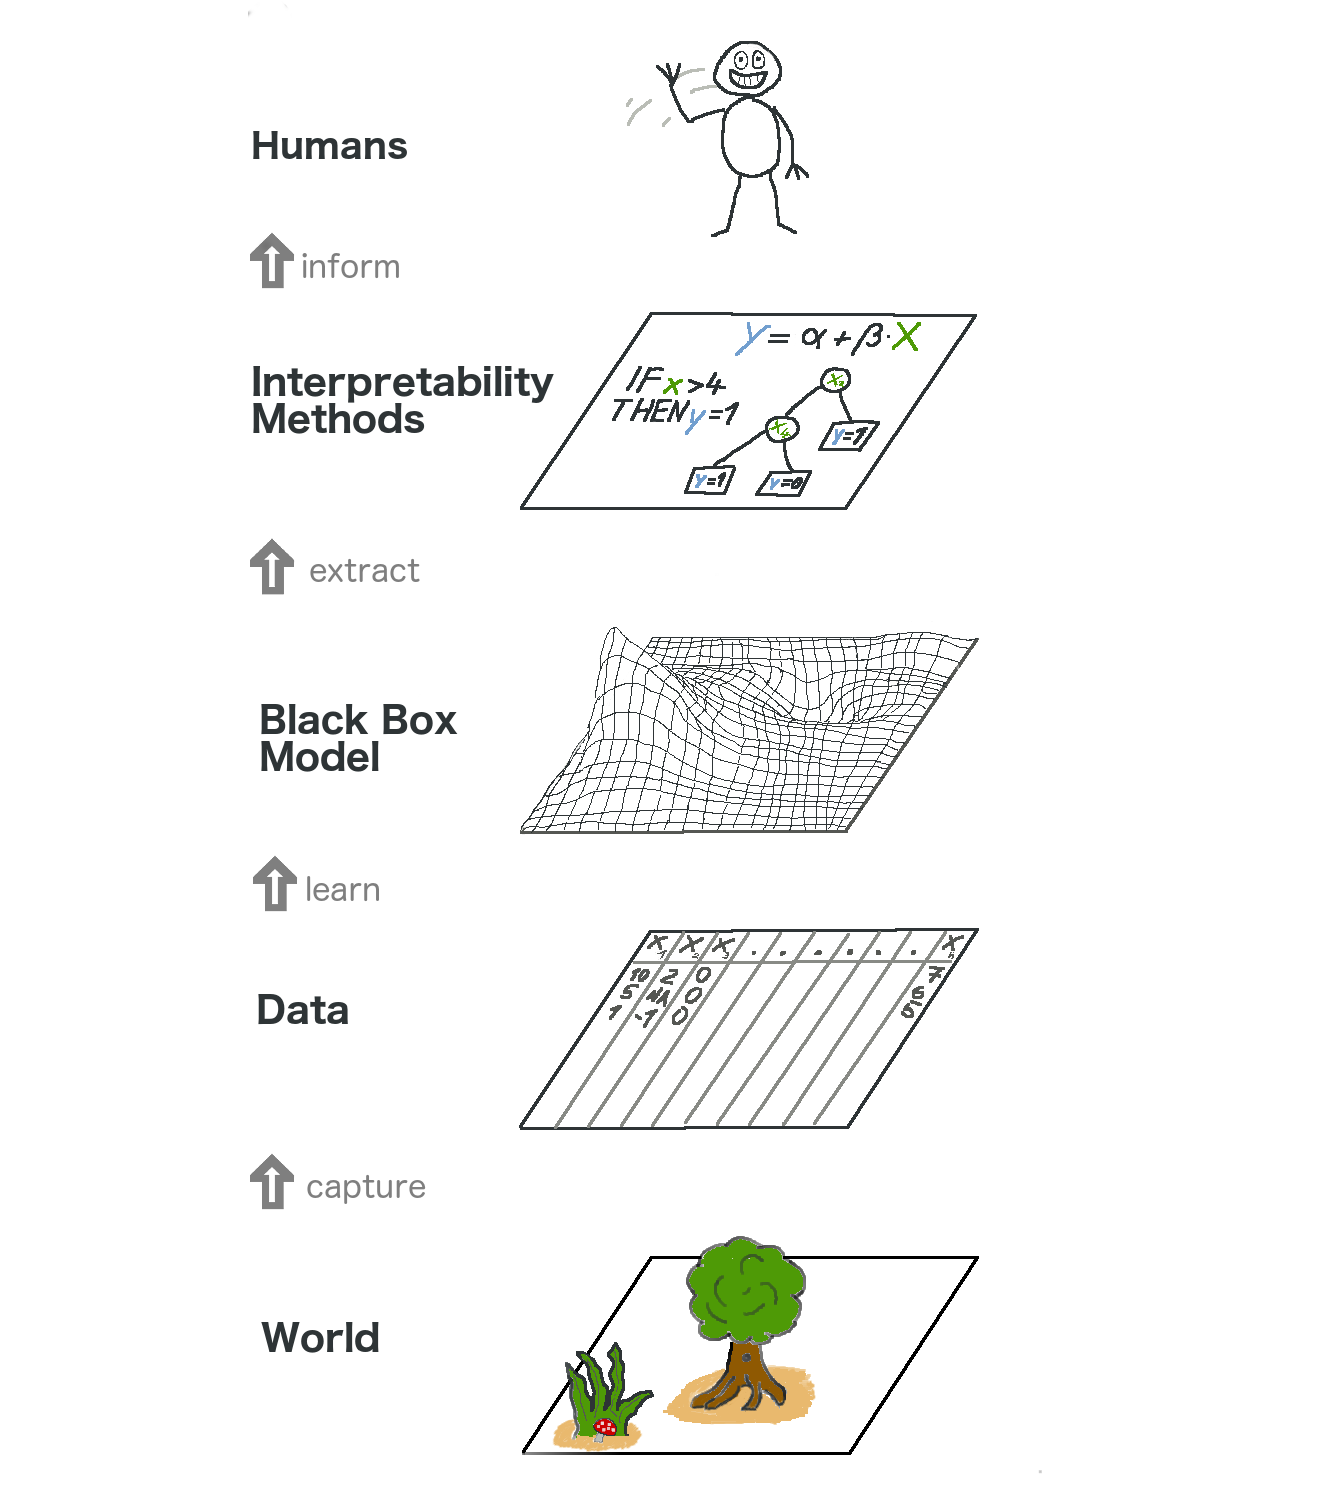
\includegraphics[width=\textwidth]{images/big-picture} 

}

\caption{The big picture of explainable machine learning. The real world goes through many layers before it reaches the human in the form of explanations.}\label{fig:bigpicture}
\end{figure}

The lowest layer is the \textbf{World}.
This could literally be nature itself, like the biology of the human body and how it reacts to medication, but also more abstract things like the real estate market.
The World layer contains everything that can be observed and is of interest.
Ultimately, we want to learn something about the World and interact with it.

The second layer is the \textbf{Data} layer.
We have to digitize the World in order to make it processable for computers and also to store information.
The Data layer contains anything from images, texts, tabular data and so on.

By fitting machine learning models based on the Data layer, we get the \textbf{Black Box Model} layer.
Machine learning algorithms learn with data from the real world to make predictions or find structures.

Above the Black Box Model layer is the \textbf{Interpretability Methods} layer, which helps us deal with the opacity of machine learning models.
What were the most important features for a particular diagnosis?
Why was a financial transaction classified as fraud?

The last layer is occupied by a \textbf{Human}.
Look! This one waves to you because you are reading this book and helping to provide better explanations for black box models!
Humans are ultimately the consumers of the explanations.

This multi-layered abstraction also helps to understand the differences in approaches between statisticians and machine learning practitioners.
Statisticians deal with the Data layer, such as planning clinical trials or designing surveys.
They skip the Black Box Model layer and go right to the Interpretability Methods layer.
Machine learning specialists also deal with the Data layer, such as collecting labeled samples of skin cancer images or crawling Wikipedia.
Then they train a black box machine learning model.
The Interpretability Methods layer is skipped and humans directly deal with the black box model predictions.
It's great that interpretable machine learning fuses the work of statisticians and machine learning specialists.

Of course this graphic does not capture everything:
Data could come from simulations.
Black box models also output predictions that might not even reach humans, but only supply other machines, and so on.
But overall it is a useful abstraction to understand how interpretability becomes this new layer on top of machine learning models.

Model-agnostic interpretation methods can be further distinguished into local and global methods.
The book is also organized according to this distinction.
\protect\hyperlink{global-methods}{Global methods} describe how features affect the prediction \textbf{on average}.
In contrast, \protect\hyperlink{local-methods}{local methods} aim to explain \textbf{individual predictions}.

\hypertarget{example-based}{%
\chapter{Example-Based Explanations}\label{example-based}}

Example-based explanation methods select particular instances of the dataset to explain the behavior of machine learning models or to explain the underlying data distribution.

Example-based explanations are mostly model-agnostic, because they make any machine learning model more interpretable.
The difference to model-agnostic methods is that the example-based methods explain a model by selecting instances of the dataset and not by creating summaries of features (such as \protect\hyperlink{feature-importance}{feature importance} or \protect\hyperlink{pdp}{partial dependence}).
Example-based explanations only make sense if we can represent an instance of the data in a humanly understandable way.
This works well for images, because we can view them directly.
In general, example-based methods work well if the feature values of an instance carry more context, meaning the data has a structure, like images or texts do.
It is more challenging to represent tabular data in a meaningful way, because an instance can consist of hundreds or thousands of (less structured) features.
Listing all feature values to describe an instance is usually not useful.
It works well if there are only a handful of features or if we have a way to summarize an instance.

Example-based explanations help humans construct mental models of the machine learning model and the data the machine learning model has been trained on.
It especially helps to understand complex data distributions.
But what do I mean by example-based explanations?
We often use them in our jobs and daily lives.
Let us start with some examples\footnote{Aamodt, Agnar, and Enric Plaza. ``Case-based reasoning: Foundational issues, methodological variations, and system approaches.'' AI communications 7.1 (1994): 39-59.}.

A physician sees a patient with an unusual cough and a mild fever.
The patient's symptoms remind her of another patient she had years ago with similar symptoms.
She suspects that her current patient could have the same disease and she takes a blood sample to test for this specific disease.

A data scientist works on a new project for one of his clients:
Analysis of the risk factors that lead to the failure of production machines for keyboards.
The data scientist remembers a similar project he worked on and reuses parts of the code from the old project because he thinks the client wants the same analysis.

A kitten sits on the window ledge of a burning and uninhabited house.
The fire department has already arrived and one of the firefighters ponders for a second whether he can risk going into the building to save the kitten.
He remembers similar cases in his life as a firefighter:
Old wooden houses that have been burning slowly for some time were often unstable and eventually collapsed.
Because of the similarity of this case, he decides not to enter, because the risk of the house collapsing is too great.
Fortunately, the kitty jumps out of the window, lands safely and nobody is harmed in the fire. Happy end.

These stories illustrate how we humans think in examples or analogies.
The blueprint of example-based explanations is:
Thing B is similar to thing A and A caused Y, so I predict that B will cause Y as well.
Implicitly, some machine learning approaches work example-based.
\protect\hyperlink{tree}{Decision trees} partition the data into nodes based on the similarities of the data points in the features that are important for predicting the target.
A decision tree gets the prediction for a new data instance by finding the instances that are similar (= in the same terminal node) and returning the average of the outcomes of those instances as the prediction.
The k-nearest neighbors (knn) method works explicitly with example-based predictions.
For a new instance, a knn model locates the k-nearest neighbors (e.g.~the k=3 closest instances) and returns the average of the outcomes of those neighbors as a prediction.
The prediction of a knn can be explained by returning the k neighbors, which -- again -- is only meaningful if we have a good way to represent a single instance.

The following interpretation methods are all example-based:

\begin{itemize}
\tightlist
\item
  \protect\hyperlink{counterfactual}{Counterfactual explanations} tell us how an instance has to change to significantly change its prediction.
  By creating counterfactual instances, we learn about how the model makes its predictions and can explain individual predictions.
\item
  \protect\hyperlink{adversarial}{Adversarial examples} are counterfactuals used to fool machine learning models.
  The emphasis is on flipping the prediction and not explaining it.
\item
  \protect\hyperlink{proto}{Prototypes} are a selection of representative instances from the data and criticisms are instances that are not well represented by those prototypes. \footnote{Kim, Been, Rajiv Khanna, and Oluwasanmi O. Koyejo. ``Examples are not enough, learn to criticize! Criticism for interpretability.'' Advances in Neural Information Processing Systems (2016).}
\item
  \protect\hyperlink{influential}{Influential instances} are the training data points that were the most influential for the parameters of a prediction model or the predictions themselves.
  Identifying and analysing influential instances helps to find problems with the data, debug the model and understand the model's behavior better.
\item
  \protect\hyperlink{other-interpretable}{k-nearest neighbors model}: An (interpretable) machine learning model based on examples.
\end{itemize}

\hypertarget{global-methods}{%
\chapter{Global Model-Agnostic Methods}\label{global-methods}}

Global methods describe the average behavior of a machine learning model.
The counterpart to global methods are \protect\hyperlink{local-methods}{local methods}.
Global methods are often expressed as expected values based on the distribution of the data.
For example, the \protect\hyperlink{pdp}{partial dependence plot}, a feature effect plot, is the expected prediction when all other features are marginalized out.
Since global interpretation methods describe average behavior, they are particularly useful when the modeler wants to understand the general mechanisms in the data or debug a model.

In this book, you will learn about the following model-agnostic global interpretation techniques:

\begin{itemize}
\tightlist
\item
  The \protect\hyperlink{pdp}{partial dependence plot} is a feature effect method.
\item
  \protect\hyperlink{ale}{Accumulated local effect plots} is another feature effect method that works when features are dependent.
\item
  \protect\hyperlink{interaction}{Feature interaction (H-statistic)} quantifies to what extent the prediction is the result of joint effects of the features.
\item
  \protect\hyperlink{decompostion}{Functional decomposition} is a central idea of interpretability and a technique that decomposes the complex prediction function into smaller parts.
\item
  \protect\hyperlink{feature-importance}{Permutation feature importance} measures the importance of a feature as an increase in loss when the feature is permuted.
\item
  \protect\hyperlink{global}{Global surrogate models} replaces the original model with a simpler model for interpretation.
\item
  \protect\hyperlink{proto}{Prototypes and criticisms} are representative data point of a distribution and can be used to enhance interpretability.
\end{itemize}

\newpage

\hypertarget{pdp}{%
\section{Partial Dependence Plot (PDP)}\label{pdp}}

The partial dependence plot (short PDP or PD plot) shows the marginal effect one or two features have on the predicted outcome of a machine learning model (J. H. Friedman 2001\footnote{Friedman, Jerome H. ``Greedy function approximation: A gradient boosting machine.'' Annals of statistics (2001): 1189-1232.}).
A partial dependence plot can show whether the relationship between the target and a feature is linear, monotonic or more complex.
For example, when applied to a linear regression model, partial dependence plots always show a linear relationship.

The partial dependence function for regression is defined as:

\[\hat{f}_{x_S}(x_S)=E_{X_C}\left[\hat{f}(x_S,X_C)\right]=\int\hat{f}(x_S,X_C)d\mathbb{P}(X_C)\]

The \(x_S\) are the features for which the partial dependence function should be plotted and \(X_C\) are the other features used in the machine learning model \(\hat{f}\), which are here treated as random variables.
Usually, there are only one or two features in the set S.
The feature(s) in S are those for which we want to know the effect on the prediction.
The feature vectors \(x_S\) and \(x_C\) combined make up the total feature space x.
Partial dependence works by marginalizing the machine learning model output over the distribution of the features in set C, so that the function shows the relationship between the features in set S we are interested in and the predicted outcome.
By marginalizing over the other features, we get a function that depends only on features in S, interactions with other features included.

The partial function \(\hat{f}_{x_S}\) is estimated by calculating averages in the training data, also known as Monte Carlo method:

\[\hat{f}_{x_S}(x_S)=\frac{1}{n}\sum_{i=1}^n\hat{f}(x_S,x^{(i)}_{C})\]
The partial function tells us for given value(s) of features S what the average marginal effect on the prediction is.
In this formula, \(x^{(i)}_{C}\) are actual feature values from the dataset for the features in which we are not interested, and n is the number of instances in the dataset.
An assumption of the PDP is that the features in C are not correlated with the features in S.
If this assumption is violated, the averages calculated for the partial dependence plot will include data points that are very unlikely or even impossible (see disadvantages).

For classification where the machine learning model outputs probabilities, the partial dependence plot displays the probability for a certain class given different values for feature(s) in S.
An easy way to deal with multiple classes is to draw one line or plot per class.

The partial dependence plot is a global method:
The method considers all instances and gives a statement about the global relationship of a feature with the predicted outcome.

\textbf{Categorical features}

So far, we have only considered numerical features.
For categorical features, the partial dependence is very easy to calculate.
For each of the categories, we get a PDP estimate by forcing all data instances to have the same category.
For example, if we look at the bike rental dataset and are interested in the partial dependence plot for the season, we get 4 numbers, one for each season.
To compute the value for ``summer'', we replace the season of all data instances with ``summer'' and average the predictions.

\hypertarget{pdp-based-feature-importance}{%
\subsection{PDP-based Feature Importance}\label{pdp-based-feature-importance}}

Greenwell et. al (2018) \footnote{Greenwell, Brandon M., Bradley C. Boehmke, and Andrew J. McCarthy. ``A simple and effective model-based variable importance measure.'' arXiv preprint arXiv:1805.04755 (2018).} proposed a simple partial dependence-based feature importance measure.
The basic motivation is that a flat PDP indicates that the feature is not important, and the more the PDP varies, the more important the feature is.
For numerical features, importance is defined as the deviation of each unique feature value from the average curve:

\[I(x_S) =  \sqrt{\frac{1}{K-1}\sum_{k=1}^K(f_S(x^{(k)}_S) - \frac{1}{K}\sum_{k=1}^K f_S({x^{(k)}_S))^2}}\]

Note that here the \(x^{(k)}_S\) are the K unique values of feature the \(X_S\).
For categorical features we have:

\[I(x_S) = (max_k(f_S(x^{(k)}_S)) - min_k(f_S(x^{(k)}_S)))/4\]

This is the range of the PDP values for the unique categories divided by four.
This strange way of calculating the deviation is called the range rule.
It helps to get a rough estimate for the deviation when you only know the range.
And the denominator four comes from the standard normal distribution:
In the normal distribution, 95\% of the data are minus two and plus two standard deviations around the mean.
So the range divided by four gives a rough estimate that probably underestimates the actual variance.

This PDP-based feature importance should be interpreted with care.
It captures only the main effect of the feature and ignores possible feature interactions.
A feature could be very important based on other methods such as \protect\hyperlink{feature-importance}{permutation feature importance}, but the PDP could be flat as the feature affects the prediction mainly through interactions with other features.
Another drawback of this measure is that it is defined over the unique values.
A unique feature value with just one instance is given the same weight in the importance computation as a value with many instances.

\hypertarget{examples}{%
\subsection{Examples}\label{examples}}

In practice, the set of features S usually only contains one feature or a maximum of two, because one feature produces 2D plots and two features produce 3D plots.
Everything beyond that is quite tricky.
Even 3D on a 2D paper or monitor is already challenging.

Let us return to the regression example, in which we predict the number of \protect\hyperlink{bike-data}{bikes that will be rented on a given day}.
First we fit a machine learning model, then we analyze the partial dependencies.
In this case, we have fitted a random forest to predict the number of bicycles and use the partial dependence plot to visualize the relationships the model has learned.
The influence of the weather features on the predicted bike counts is visualized in the following figure.

\begin{figure}

{\centering \includegraphics[width=\textwidth]{images/pdp-bike-1} 

}

\caption{PDPs for the bicycle count prediction model and temperature, humidity and wind speed. The largest differences can be seen in the temperature. The hotter, the more bikes are rented. This trend goes up to 20 degrees Celsius, then flattens and drops slightly at 30. Marks on the x-axis indicate the data distribution.}\label{fig:pdp-bike}
\end{figure}

For warm but not too hot weather, the model predicts on average a high number of rented bicycles.
Potential bikers are increasingly inhibited in renting a bike when humidity exceeds 60\%.
In addition, the more wind the fewer people like to cycle, which makes sense.
Interestingly, the predicted number of bike rentals does not fall when wind speed increases from 25 to 35 km/h, but there is not much training data, so the machine learning model could probably not learn a meaningful prediction for this range.
At least intuitively, I would expect the number of bicycles to decrease with increasing wind speed, especially when the wind speed is very high.

To illustrate a partial dependence plot with a categorical feature, we examine the effect of the season feature on the predicted bike rentals.

\begin{figure}

{\centering 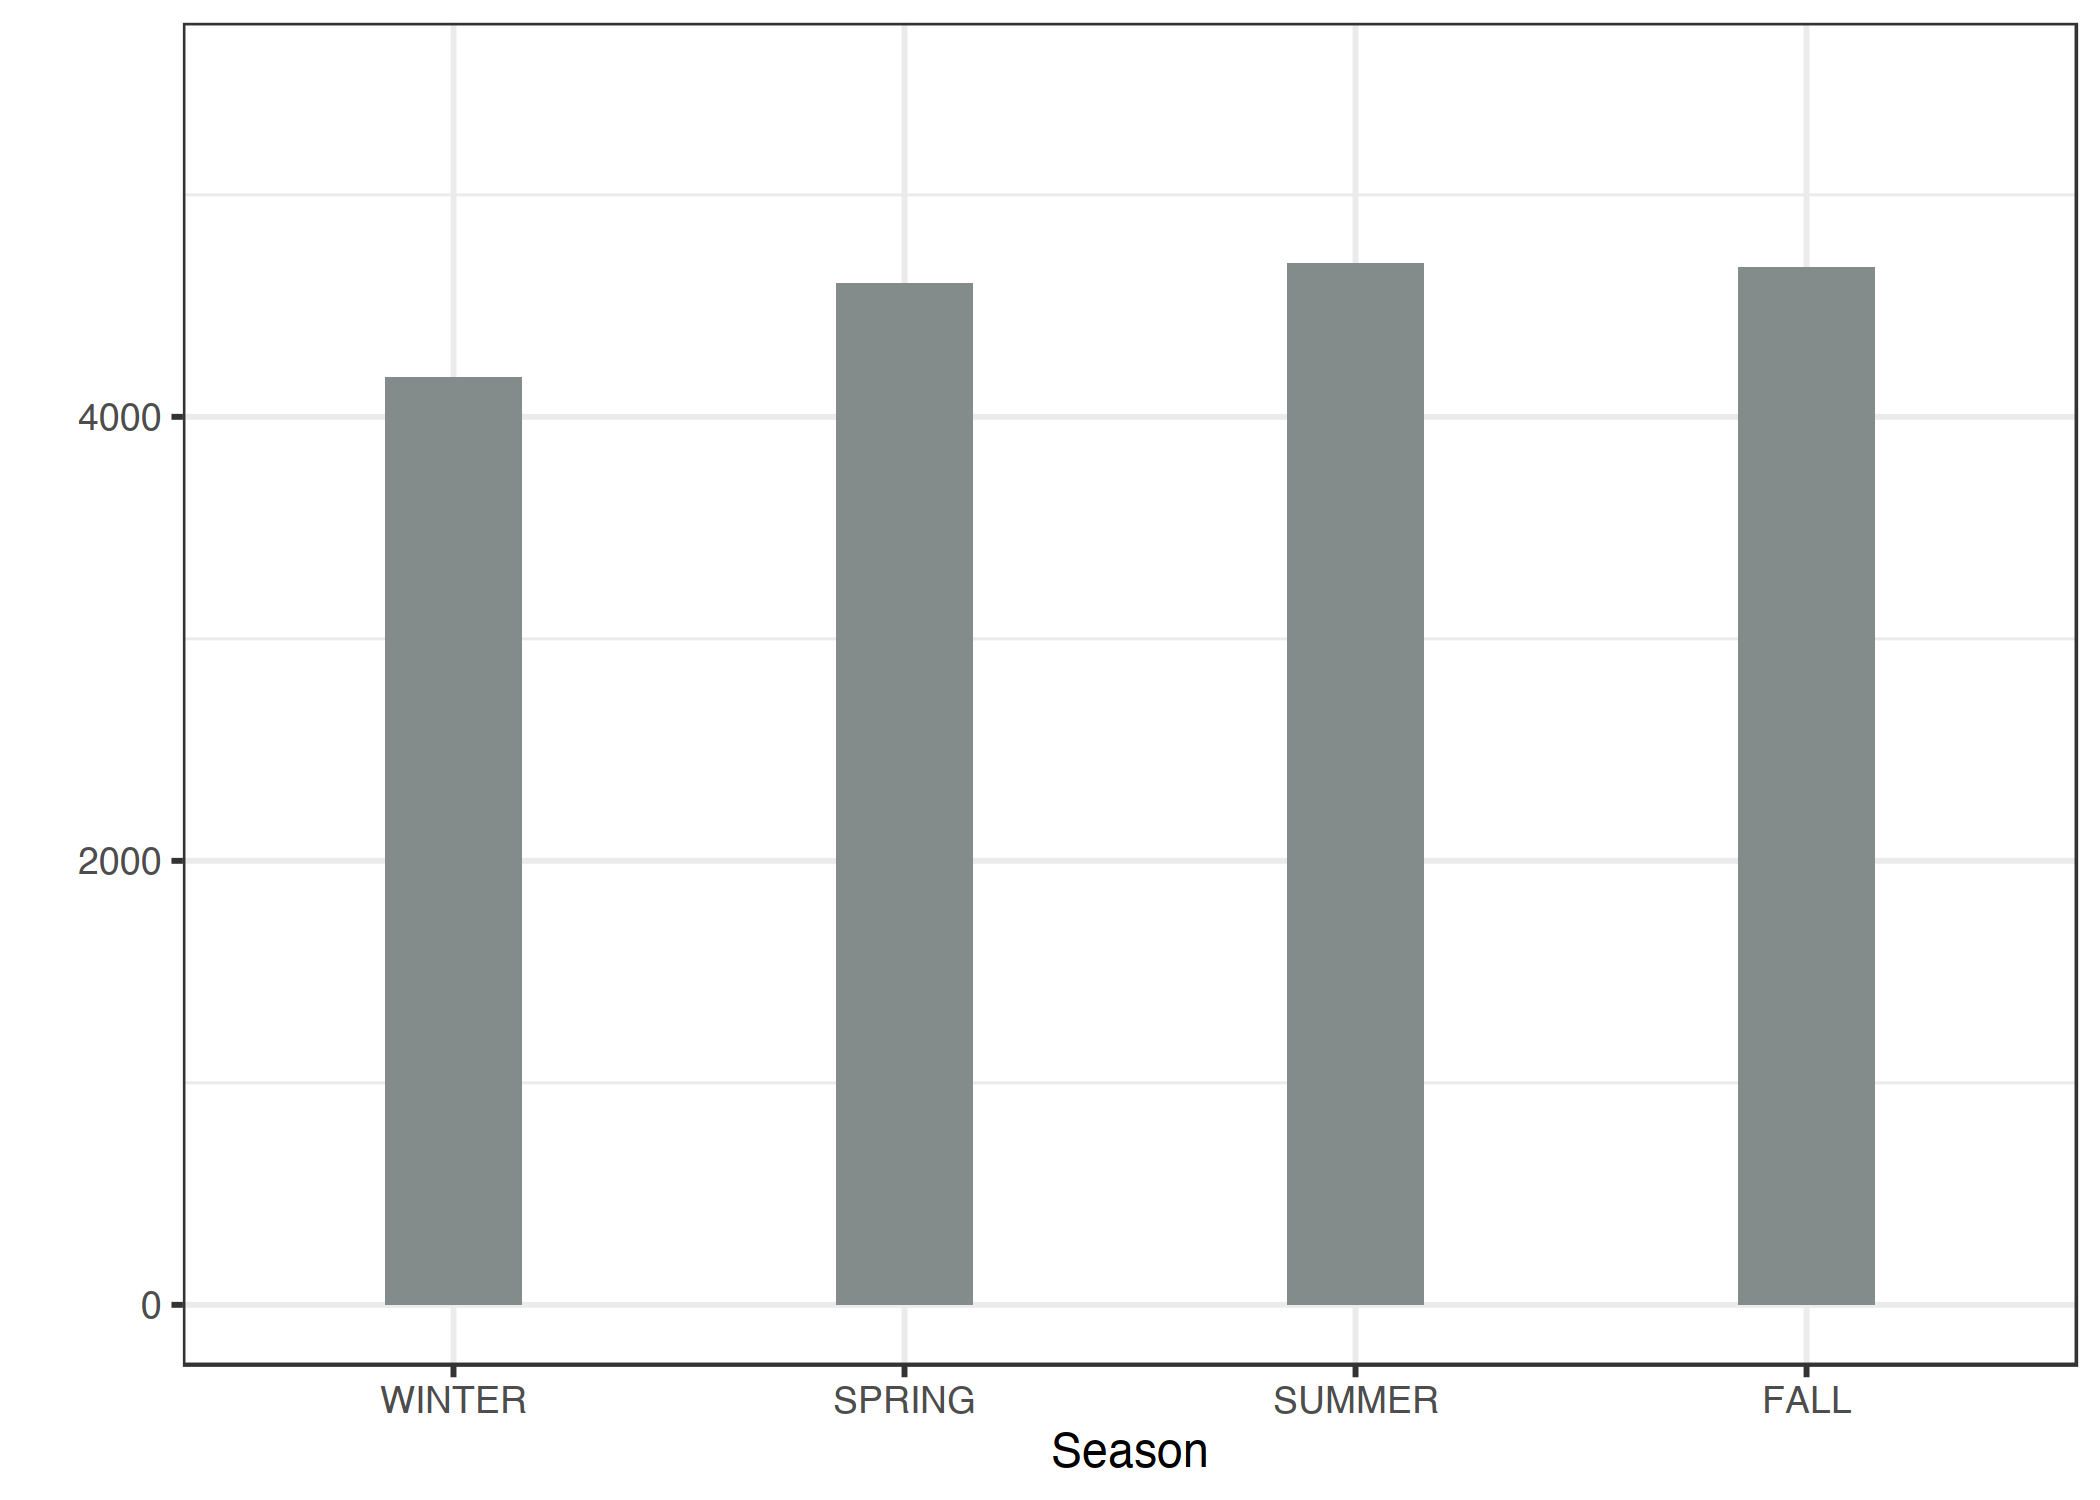
\includegraphics[width=\textwidth]{images/pdp-bike-cat-1} 

}

\caption{PDPs for the bike count prediction model and the season. Unexpectedly all seasons show similar effect on the model predictions, only for spring the model predicts fewer bicycle rentals.}\label{fig:pdp-bike-cat}
\end{figure}

We also compute the partial dependence for \protect\hyperlink{cervical}{cervical cancer classification}.
This time we fit a random forest to predict whether a woman might get cervical cancer based on risk factors.
We compute and visualize the partial dependence of the cancer probability on different features for the random forest:

\begin{figure}

{\centering \includegraphics[width=\textwidth]{images/pdp-cervical-1} 

}

\caption{PDPs of cancer probability based on age and years with hormonal contraceptives. For age, the PDP shows that the probability is low until 40 and increases after. The more years on hormonal contraceptives the higher the predicted cancer risk, especially after 10 years. For both features not many data points with large values were available, so the PD estimates are less reliable in those regions.}\label{fig:pdp-cervical}
\end{figure}

We can also visualize the partial dependence of two features at once:

\begin{figure}

{\centering \includegraphics[width=\textwidth]{images/pdp-cervical-2d-1} 

}

\caption{PDP of cancer probability and the interaction of age and number of pregnancies. The plot shows the increase in cancer probability at 45. For ages below 25, women who had 1 or 2 pregnancies have a lower predicted cancer risk, compared with women who had 0 or more than 2 pregnancies. But be careful when drawing conclusions: This might just be a correlation and not causal!}\label{fig:pdp-cervical-2d}
\end{figure}

\hypertarget{advantages-5}{%
\subsection{Advantages}\label{advantages-5}}

The computation of partial dependence plots is \textbf{intuitive}:
The partial dependence function at a particular feature value represents the average prediction if we force all data points to assume that feature value.
In my experience, lay people usually understand the idea of PDPs quickly.

If the feature for which you computed the PDP is not correlated with the other features, then the PDPs perfectly represent how the feature influences the prediction on average.
In the uncorrelated case, the \textbf{interpretation is clear}:
The partial dependence plot shows how the average prediction in your dataset changes when the j-th feature is changed.
It is more complicated when features are correlated, see also disadvantages.

Partial dependence plots are \textbf{easy to implement}.

The calculation for the partial dependence plots has a \textbf{causal interpretation}.
We intervene on a feature and measure the changes in the predictions.
In doing so, we analyze the causal relationship between the feature and the prediction.\footnote{Zhao, Qingyuan, and Trevor Hastie. ``Causal interpretations of black-box models.'' Journal of Business \& Economic Statistics, to appear. (2017).}
The relationship is causal for the model -- because we explicitly model the outcome as a function of the features -- but not necessarily for the real world!

\hypertarget{disadvantages-5}{%
\subsection{Disadvantages}\label{disadvantages-5}}

The realistic \textbf{maximum number of features} in a partial dependence function is two.
This is not the fault of PDPs, but of the 2-dimensional representation (paper or screen) and also of our inability to imagine more than 3 dimensions.

Some PD plots do not show the \textbf{feature distribution}.
Omitting the distribution can be misleading, because you might overinterpret regions with almost no data.
This problem is easily solved by showing a rug (indicators for data points on the x-axis) or a histogram.

The \textbf{assumption of independence} is the biggest issue with PD plots.
It is assumed that the feature(s) for which the partial dependence is computed are not correlated with other features.
For example, suppose you want to predict how fast a person walks, given the person's weight and height.
For the partial dependence of one of the features, e.g.~height, we assume that the other features (weight) are not correlated with height, which is obviously a false assumption.
For the computation of the PDP at a certain height (e.g.~200 cm), we average over the marginal distribution of weight, which might include a weight below 50 kg, which is unrealistic for a 2 meter person.
In other words:
When the features are correlated, we create new data points in areas of the feature distribution where the actual probability is very low (for example it is unlikely that someone is 2 meters tall but weighs less than 50 kg).
One solution to this problem is \protect\hyperlink{ale}{Accumulated Local Effect plots} or short ALE plots that work with the conditional instead of the marginal distribution.

\textbf{Heterogeneous effects might be hidden} because PD plots only show the average marginal effects.
Suppose that for a feature half your data points have a positive association with the prediction -- the larger the feature value the larger the prediction -- and the other half has a negative association -- the smaller the feature value the larger the prediction.
The PD curve could be a horizontal line, since the effects of both halves of the dataset could cancel each other out.
You then conclude that the feature has no effect on the prediction.
By plotting the \protect\hyperlink{ice}{individual conditional expectation curves} instead of the aggregated line, we can uncover heterogeneous effects.

\hypertarget{software-and-alternatives-1}{%
\subsection{Software and Alternatives}\label{software-and-alternatives-1}}

There are a number of R packages that implement PDPs.
I used the \texttt{iml} package for the examples, but there is also \texttt{pdp} or \texttt{DALEX}.
In Python, partial dependence plots are built into \texttt{scikit-learn} and you can use \texttt{PDPBox}.

Alternatives to PDPs presented in this book are \protect\hyperlink{ale}{ALE plots} and \protect\hyperlink{ice}{ICE curves}.

\newpage

\hypertarget{ale}{%
\section{Accumulated Local Effects (ALE) Plot}\label{ale}}

Accumulated local effects\footnote{Apley, Daniel W., and Jingyu Zhu. ``Visualizing the effects of predictor variables in black box supervised learning models.'' Journal of the Royal Statistical Society: Series B (Statistical Methodology) 82.4 (2020): 1059-1086.} describe how features influence the prediction of a machine learning model on average.
ALE plots are a faster and unbiased alternative to partial dependence plots (PDPs).

I recommend reading the \protect\hyperlink{pdp}{chapter on partial dependence plots} first, as they are easier to understand and both methods share the same goal:
Both describe how a feature affects the prediction on average.
In the following section, I want to convince you that partial dependence plots have a serious problem when the features are correlated.

\hypertarget{motivation-and-intuition}{%
\subsection{Motivation and Intuition}\label{motivation-and-intuition}}

If features of a machine learning model are correlated, the partial dependence plot cannot be trusted.
The computation of a partial dependence plot for a feature that is strongly correlated with other features involves averaging predictions of artificial data instances that are unlikely in reality.
This can greatly bias the estimated feature effect.
Imagine calculating partial dependence plots for a machine learning model that predicts the value of a house depending on the number of rooms and the size of the living area.
We are interested in the effect of the living area on the predicted value.
As a reminder, the recipe for partial dependence plots is: 1) Select feature. 2) Define grid. 3) Per grid value: a) Replace feature with grid value and b) average predictions. 4) Draw curve.
For the calculation of the first grid value of the PDP -- say 30 m\textsuperscript{2} -- we replace the living area for \textbf{all} instances by 30 m\textsuperscript{2}, even for houses with 10 rooms.
Sounds to me like a very unusual house.
The partial dependence plot includes these unrealistic houses in the feature effect estimation and pretends that everything is fine.
The following figure illustrates two correlated features and how it comes that the partial dependence plot method averages predictions of unlikely instances.

\begin{figure}

{\centering \includegraphics[width=\textwidth]{images/aleplot-motivation1-1} 

}

\caption{Strongly correlated features x1 and x2. To calculate the feature effect of x1 at 0.75, the PDP replaces x1 of all instances with 0.75, falsely assuming that the distribution of x2 at x1 = 0.75 is the same as the marginal distribution of x2 (vertical line). This results in unlikely combinations of x1 and x2 (e.g. x2=0.2 at x1=0.75), which the PDP uses for the calculation of the average effect.}\label{fig:aleplot-motivation1}
\end{figure}

What can we do to get a feature effect estimate that respects the correlation of the features?
We could average over the conditional distribution of the feature, meaning at a grid value of x1, we average the predictions of instances with a similar x1 value.
The solution for calculating feature effects using the conditional distribution is called Marginal Plots, or M-Plots (confusing name, since they are based on the conditional, not the marginal distribution).
Wait, did I not promise you to talk about ALE plots?
M-Plots are not the solution we are looking for.
Why do M-Plots not solve our problem?
If we average the predictions of all houses of about 30 m\textsuperscript{2}, we estimate the \textbf{combined} effect of living area and of number of rooms, because of their correlation.
Suppose that the living area has no effect on the predicted value of a house, only the number of rooms has.
The M-Plot would still show that the size of the living area increases the predicted value, since the number of rooms increases with the living area.
The following plot shows for two correlated features how M-Plots work.

\begin{figure}

{\centering \includegraphics[width=\textwidth]{images/aleplot-motivation2-1} 

}

\caption{Strongly correlated features x1 and x2. M-Plots average over the conditional distribution. Here the conditional distribution of x2 at x1 = 0.75. Averaging the local predictions leads to mixing the effects of both features.}\label{fig:aleplot-motivation2}
\end{figure}

M-Plots avoid averaging predictions of unlikely data instances, but they mix the effect of a feature with the effects of all correlated features.
ALE plots solve this problem by calculating -- also based on the conditional distribution of the features -- \textbf{differences in predictions instead of averages}.
For the effect of living area at 30 m\textsuperscript{2}, the ALE method uses all houses with about 30 m\textsuperscript{2}, gets the model predictions pretending these houses were 31 m\textsuperscript{2} minus the prediction pretending they were 29 m\textsuperscript{2}.
This gives us the pure effect of the living area and is not mixing the effect with the effects of correlated features.
The use of differences blocks the effect of other features.
The following graphic provides intuition how ALE plots are calculated.

\begin{figure}

{\centering \includegraphics[width=\textwidth]{images/aleplot-computation-1} 

}

\caption{Calculation of ALE for feature x1, which is correlated with x2. First, we divide the feature into intervals (vertical lines). For the data instances (points) in an interval, we calculate the difference in the prediction when we replace the feature with the upper and lower limit of the interval (horizontal lines). These differences are later accumulated and centered, resulting in the ALE curve.}\label{fig:aleplot-computation}
\end{figure}

To summarize how each type of plot (PDP, M, ALE) calculates the effect of a feature at a certain grid value v:\\
\textbf{Partial Dependence Plots}: ``Let me show you what the model predicts on average when each data instance has the value v for that feature.
I ignore whether the value v makes sense for all data instances.''\\
\textbf{M-Plots}: ``Let me show you what the model predicts on average for data instances that have values close to v for that feature.
The effect could be due to that feature, but also due to correlated features.''\\
\textbf{ALE plots}: ``Let me show you how the model predictions change in a small''window" of the feature around v for data instances in that window."

\hypertarget{theory-2}{%
\subsection{Theory}\label{theory-2}}

How do PD, M and ALE plots differ mathematically?
Common to all three methods is that they reduce the complex prediction function f to a function that depends on only one (or two) features.
All three methods reduce the function by averaging the effects of the other features, but they differ in whether averages of predictions or of \textbf{differences in predictions} are calculated and whether averaging is done over the marginal or conditional distribution.

Partial dependence plots average the predictions over the marginal distribution.

\begin{align*}
\hat{f}_{S,PDP}(x)&=E_{X_C}\left[\hat{f}(x_S,X_C)\right] \\
& = \int_{X_C}\hat{f}(x_S,X_C)d\mathbb{P}(X_C)
\end{align*}

This is the value of the prediction function f, at feature value(s) \(x_S\), averaged over all features in \(X_C\) (here treated as random variables).
Averaging means calculating the marginal expectation E over the features in set C, which is the integral over the predictions weighted by the probability distribution.
Sounds fancy, but to calculate the expected value over the marginal distribution, we simply take all our data instances, force them to have a certain grid value for the features in set S, and average the predictions for this manipulated dataset.
This procedure ensures that we average over the marginal distribution of the features.

M-plots average the predictions over the conditional distribution.

\begin{align*}\hat{f}_{S,M}(x_S)&=E_{X_C|X_S}\left[\hat{f}(X_S,X_C)|X_S=x_s\right]\\&=\int_{X_C}\hat{f}(x_S, X_C)d\mathbb{P}(X_C|X_S = x_S)\end{align*}

The only thing that changes compared to PDPs is that we average the predictions conditional on each grid value of the feature of interest, instead of assuming the marginal distribution at each grid value.
In practice, this means that we have to define a neighborhood, for example for the calculation of the effect of 30 m\textsuperscript{2} on the predicted house value, we could average the predictions of all houses between 28 and 32 m\textsuperscript{2}.

ALE plots average the changes in the predictions and accumulate them over the grid (more on the calculation later).

\begin{align*}
\hat{f}_{S,ALE}(x_S)=&\int_{z_{0,S}}^{x_S}E_{X_C|X_S = x_S}\left[\hat{f}^S(X_s,X_c)|X_S=z_S\right]dz_S-\text{constant}\\
 = & \int_{z_{0,S}}^{x_S}(\int_{x_C}\hat{f}^S(z_s,X_c)d\mathbb{P}(X_C|X_S = z_S)d{})dz_S-\text{constant}
\end{align*}

The formula reveals three differences to M-Plots.
First, we average the changes of predictions, not the predictions itself.
The change is defined as the partial derivative (but later, for the actual computation, replaced by the differences in the predictions over an interval).

\[\hat{f}^S(x_s,x_c)=\frac{\partial\hat{f}(x_S,x_C)}{\partial{}x_S}\]

The second difference is the additional integral over z.
We accumulate the local partial derivatives over the range of features in set S, which gives us the effect of the feature on the prediction.
For the actual computation, the z's are replaced by a grid of intervals over which we compute the changes in the prediction.
Instead of directly averaging the predictions, the ALE method calculates the prediction differences conditional on features S and integrates the derivative over features S to estimate the effect.
Well, that sounds stupid.
Derivation and integration usually cancel each other out, like first subtracting, then adding the same number.
Why does it make sense here?
The derivative (or interval difference) isolates the effect of the feature of interest and blocks the effect of correlated features.

The third difference of ALE plots to M-plots is that we subtract a constant from the results.
This step centers the ALE plot so that the average effect over the data is zero.

One problem remains:
Not all models come with a gradient, for example random forests have no gradient.
But as you will see, the actual computation works without gradients and uses intervals.
Let us delve a little deeper into the estimation of ALE plots.

\hypertarget{estimation}{%
\subsection{Estimation}\label{estimation}}

First I will describe how ALE plots are estimated for a single numerical feature, later for two numerical features and for a single categorical feature.
To estimate local effects, we divide the feature into many intervals and compute the differences in the predictions.
This procedure approximates the derivatives and also works for models without derivatives.

First we estimate the uncentered effect:

\[\hat{\tilde{f}}_{j,ALE}(x)=\sum_{k=1}^{k_j(x)}\frac{1}{n_j(k)}\sum_{i:x_{j}^{(i)}\in{}N_j(k)}\left[f(z_{k,j},x^{(i)}_{\setminus{}j})-f(z_{k-1,j},x^{(i)}_{\setminus{}j})\right]\]

Let us break this formula down, starting from the right side.
The name \textbf{Accumulated Local Effects} nicely reflects all the individual components of this formula.
At its core, the ALE method calculates the differences in predictions, whereby we replace the feature of interest with grid values z.
The difference in prediction is the \textbf{Effect} the feature has for an individual instance in a certain interval.
The sum on the right adds up the effects of all instances within an interval which appears in the formula as neighborhood \(N_j(k)\).
We divide this sum by the number of instances in this interval to obtain the average difference of the predictions for this interval.
This average in the interval is covered by the term \textbf{Local} in the name ALE.
The left sum symbol means that we accumulate the average effects across all intervals.
The (uncentered) ALE of a feature value that lies, for example, in the third interval is the sum of the effects of the first, second and third intervals.
The word \textbf{Accumulated} in ALE reflects this.

This effect is centered so that the mean effect is zero.

\[\hat{f}_{j,ALE}(x)=\hat{\tilde{f}}_{j,ALE}(x)-\frac{1}{n}\sum_{i=1}^{n}\hat{\tilde{f}}_{j,ALE}(x^{(i)}_{j})\]

The value of the ALE can be interpreted as the main effect of the feature at a certain value compared to the average prediction of the data.
For example, an ALE estimate of -2 at \(x_j=3\) means that when the j-th feature has value 3, then the prediction is lower by 2 compared to the average prediction.

The quantiles of the distribution of the feature are used as the grid that defines the intervals.
Using the quantiles ensures that there is the same number of data instances in each of the intervals.
Quantiles have the disadvantage that the intervals can have very different lengths.
This can lead to some weird ALE plots if the feature of interest is very skewed, for example many low values and only a few very high values.

\textbf{ALE plots for the interaction of two features}

ALE plots can also show the interaction effect of two features.
The calculation principles are the same as for a single feature, but we work with rectangular cells instead of intervals, because we have to accumulate the effects in two dimensions.
In addition to adjusting for the overall mean effect, we also adjust for the main effects of both features.
This means that ALE for two features estimate the second-order effect, which does not include the main effects of the features.
In other words, ALE for two features only shows the additional interaction effect of the two features.
I spare you the formulas for 2D ALE plots because they are long and unpleasant to read.
If you are interested in the calculation, I refer you to the paper, formulas (13) -- (16).
I will rely on visualizations to develop intuition about the second-order ALE calculation.

\begin{figure}

{\centering \includegraphics[width=\textwidth]{images/aleplot-computation-2d-1} 

}

\caption{Calculation of 2D-ALE. We place a grid over the two features. In each grid cell we calculate the 2nd-order differences for all instance within. We first replace values of x1 and x2 with the values from the cell corners. If a, b, c and d represent the "corner"-predictions of a manipulated instance (as labeled in the graphic), then the 2nd-order difference is (d - c) - (b - a). The mean 2nd-order difference in each cell is accumulated over the grid and centered.}\label{fig:aleplot-computation-2d}
\end{figure}

In the previous figure, many cells are empty due to the correlation.
In the ALE plot this can be visualized with a grayed out or darkened box.
Alternatively, you can replace the missing ALE estimate of an empty cell with the ALE estimate of the nearest non-empty cell.

Since the ALE estimates for two features only show the second-order effect of the features, the interpretation requires special attention.
The second-order effect is the additional interaction effect of the features after we have accounted for the main effects of the features.
Suppose two features do not interact, but each has a linear effect on the predicted outcome.
In the 1D ALE plot for each feature, we would see a straight line as the estimated ALE curve.
But when we plot the 2D ALE estimates, they should be close to zero, because the second-order effect is only the additional effect of the interaction.
ALE plots and PD plots differ in this regard:
PDPs always show the total effect, ALE plots show the first- or second-order effect.
These are design decisions that do not depend on the underlying math.
You can subtract the lower-order effects in a partial dependence plot to get the pure main or second-order effects or, you can get an estimate of the total ALE plots by refraining from subtracting the lower-order effects.

The accumulated local effects could also be calculated for arbitrarily higher orders (interactions of three or more features), but as argued in the \protect\hyperlink{pdp}{PDP chapter}, only up to two features makes sense, because higher interactions cannot be visualized or even interpreted meaningfully.

\textbf{ALE for categorical features}

The accumulated local effects method needs -- by definition -- the feature values to have an order, because the method accumulates effects in a certain direction.
Categorical features do not have any natural order.
To compute an ALE plot for a categorical feature we have to somehow create or find an order.
The order of the categories influences the calculation and interpretation of the accumulated local effects.

One solution is to order the categories according to their similarity based on the other features.
The distance between two categories is the sum over the distances of each feature.
The feature-wise distance compares either the cumulative distribution in both categories, also called Kolmogorov-Smirnov distance (for numerical features) or the relative frequency tables (for categorical features).
Once we have the distances between all categories, we use multi-dimensional scaling to reduce the distance matrix to a one-dimensional distance measure.
This gives us a similarity-based order of the categories.

To make this a little bit clearer, here is one example:
Let us assume we have the two categorical features ``season'' and ``weather'' and a numerical feature ``temperature''.
For the first categorical feature (season) we want to calculate the ALEs.
The feature has the categories ``spring'', ``summer'', ``fall'', ``winter''.
We start to calculate the distance between categories ``spring'' and ``summer''.
The distance is the sum of distances over the features temperature and weather.
For the temperature, we take all instances with season ``spring'', calculate the empirical cumulative distribution function and do the same for instances with season ``summer'' and measure their distance with the Kolmogorov-Smirnov statistic.
For the weather feature we calculate for all ``spring'' instances the probabilities for each weather type, do the same for the ``summer'' instances and sum up the absolute distances in the probability distribution.
If ``spring'' and ``summer'' have very different temperatures and weather, the total category-distance is large.
We repeat the procedure with the other seasonal pairs and reduce the resulting distance matrix to a single dimension by multi-dimensional scaling.

\hypertarget{examples-1}{%
\subsection{Examples}\label{examples-1}}

Let us see ALE plots in action.
I have constructed a scenario in which partial dependence plots fail.
The scenario consists of a prediction model and two strongly correlated features.
The prediction model is mostly a linear regression model, but does something weird at a combination of the two features for which we have never observed instances.

\begin{figure}

{\centering \includegraphics[width=\textwidth]{images/correlation-problem-1} 

}

\caption{Two features and the predicted outcome. The model predicts the sum of the two features (shaded background), with the exception that if x1 is greater than 0.7 and x2 less than 0.3, the model always predicts 2. This area is far from the distribution of data (point cloud) and does not affect the performance of the model and also should not affect its interpretation.}\label{fig:correlation-problem}
\end{figure}

Is this a realistic, relevant scenario at all?
When you train a model, the learning algorithm minimizes the loss for the existing training data instances.
Weird stuff can happen outside the distribution of training data, because the model is not penalized for doing weird stuff in these areas.
Leaving the data distribution is called extrapolation, which can also be used to fool machine learning models, described in the \protect\hyperlink{adversarial}{chapter on adversarial examples}.
See in our little example how the partial dependence plots behave compared to ALE plots.

\begin{figure}

{\centering \includegraphics[width=\textwidth]{images/correlation-pdp-ale-plot-1} 

}

\caption{Comparison of the feature effects computed with PDP (upper row) and ALE (lower row). The PDP estimates are influenced by the odd behavior of the model outside the data distribution (steep jumps in the plots). The ALE plots correctly identify that the machine learning model has a linear relationship between features and prediction, ignoring areas without data.}\label{fig:correlation-pdp-ale-plot}
\end{figure}

But is it not interesting to see that our model behaves oddly at x1 \textgreater{} 0.7 and x2 \textless{} 0.3?
Well, yes and no.
Since these are data instances that might be physically impossible or at least extremely unlikely, it is usually irrelevant to look into these instances.
But if you suspect that your test distribution might be slightly different and some instances are actually in that range, then it would be interesting to include this area in the calculation of feature effects.
But it has to be a conscious decision to include areas where we have not observed data yet and it should not be a side-effect of the method of choice like PDP.
If you suspect that the model will later be used with differently distributed data, I recommend to use ALE plots and simulate the distribution of data you are expecting.

Turning to a real dataset, let us predict the \protect\hyperlink{bike-data}{number of rented bikes} based on weather and day and check if the ALE plots really work as well as promised.
We train a regression tree to predict the number of rented bicycles on a given day and use ALE plots to analyze how temperature, relative humidity and wind speed influence the predictions.
Let us look at what the ALE plots say:

\begin{figure}

{\centering \includegraphics[width=\textwidth]{images/ale-bike-1} 

}

\caption{ALE plots for the bike prediction model by temperature, humidity and wind speed. The temperature has a strong effect on the prediction. The average prediction rises with increasing temperature, but falls again above 25 degrees Celsius. Humidity has a negative effect: When above 60\%, the higher the relative humidity, the lower the prediction. The wind speed does not affect the predictions much.}\label{fig:ale-bike}
\end{figure}

Let us look at the correlation between temperature, humidity and wind speed and all other features.
Since the data also contains categorical features, we cannot only use the Pearson correlation coefficient, which only works if both features are numerical.
Instead, I train a linear model to predict, for example, temperature based on one of the other features as input.
Then I measure how much variance the other feature in the linear model explains and take the square root.
If the other feature was numerical, then the result is equal to the absolute value of the standard Pearson correlation coefficient.
But this model-based approach of ``variance-explained'' (also called ANOVA, which stands for ANalysis Of VAriance) works even if the other feature is categorical.
The ``variance-explained'' measure lies always between 0 (no association) and 1 (temperature can be perfectly predicted from the other feature).
We calculate the explained variance of temperature, humidity and wind speed with all the other features.
The higher the explained variance (correlation), the more (potential) problems with PD plots.
The following figure visualizes how strongly the weather features are correlated with other features.

\begin{figure}

{\centering \includegraphics[width=\textwidth]{images/ale-bike-cor-1} 

}

\caption{The strength of the correlation between temperature, humidity and wind speed with all features, measured as the amount of variance explained, when we train a linear model with e.g. temperature to predict and season as feature. For temperature we observe -- not surprisingly -- a high correlation with season and month. Humidity correlates with weather situation.}\label{fig:ale-bike-cor}
\end{figure}

This correlation analysis reveals that we may encounter problems with partial dependence plots, especially for the temperature feature.
Well, see for yourself:

\begin{figure}

{\centering \includegraphics[width=\textwidth]{images/pdp-bike-compare-1} 

}

\caption{PDPs for temperature, humidity and wind speed. Compared to the ALE plots, the PDPs show a smaller decrease in predicted number of bikes for high temperature or high humidity. The PDP uses all data instances to calculate the effect of high temperatures, even if they are, for example, instances with the season "winter". The ALE plots are more reliable.}\label{fig:pdp-bike-compare}
\end{figure}

Next, let us see ALE plots in action for a categorical feature.
The month is a categorical feature for which we want to analyze the effect on the predicted number of bikes.
Arguably, the months already have a certain order (January to December), but let us try to see what happens if we first reorder the categories by similarity and then compute the effects.
The months are ordered by the similarity of days of each month based on the other features, such as temperature or whether it is a holiday.

\begin{figure}

{\centering \includegraphics[width=\textwidth]{images/ale-bike-cat-1} 

}

\caption{ALE plot for the categorical feature month. The months are ordered by their similarity to each other, based on the distributions of the other features by month. We observe that January, March and April, but especially December and November, have a lower effect on the predicted number of rented bikes compared to the other months.}\label{fig:ale-bike-cat}
\end{figure}

Since many of the features are related to weather, the order of the months strongly reflects how similar the weather is between the months.
All colder months are on the left side (February to April) and the warmer months on the right side (October to August).
Keep in mind that non-weather features have also been included in the similarity calculation, for example relative frequency of holidays has the same weight as the temperature for calculating the similarity between the months.

Next, we consider the second-order effect of humidity and temperature on the predicted number of bikes.
Remember that the second-order effect is the additional interaction effect of the two features and does not include the main effects.
This means that, for example, you will not see the main effect that high humidity leads to a lower number of predicted bikes on average in the second-order ALE plot.

\begin{figure}

{\centering \includegraphics[width=\textwidth]{images/ale-bike-2d-1} 

}

\caption{ALE plot for the 2nd-order effect of humidity and temperature on the predicted number of rented bikes. Lighter shade indicates an above average and darker shade a below average prediction when the main effects are already taken into account. The plot reveals an interaction between temperature and humidity: Hot and humid weather increases the prediction. In cold and humid weather an additional negative effect on the number of predicted bikes is shown.}\label{fig:ale-bike-2d}
\end{figure}

Keep in mind that both main effects of humidity and temperature say that the predicted number of bikes decreases in very hot and humid weather.
In hot and humid weather, the combined effect of temperature and humidity is therefore not the sum of the main effects, but larger than the sum.
To emphasize the difference between the pure second-order effect (the 2D ALE plot you just saw) and the total effect, let us look at the partial dependence plot.
The PDP shows the total effect, which combines the mean prediction, the two main effects and the second-order effect (the interaction).

\begin{figure}

{\centering \includegraphics[width=\textwidth]{images/pdp-bike-vs-ale-2D-1} 

}

\caption{PDP of the total effect of temperature and humidity on the predicted number of bikes. The plot combines the main effect of each of the features and their interaction effect, as opposed to the 2D-ALE plot which only shows the interaction.}\label{fig:pdp-bike-vs-ale-2D}
\end{figure}

If you are only interested in the interaction, you should look at the second-order effects, because the total effect mixes the main effects into the plot.
But if you want to know the combined effect of the features, you should look at the total effect (which the PDP shows).
For example, if you want to know the expected number of bikes at 30 degrees Celsius and 80 percent humidity, you can read it directly from the 2D PDP.
If you want to read the same from the ALE plots, you need to look at three plots:
The ALE plot for temperature, for humidity and for temperature + humidity and you also need to know the overall mean prediction.
In a scenario where two features have no interaction, the total effect plot of the two features could be misleading because it probably shows a complex landscape, suggesting some interaction, but it is simply the product of the two main effects.
The second-order effect would immediately show that there is no interaction.

Enough bicycles for now, let's turn to a classification task.
We train a random forest to predict the probability of \protect\hyperlink{cervical}{cervical cancer} based on risk factors.
We visualize the accumulated local effects for two of the features:

\begin{figure}

{\centering \includegraphics[width=\textwidth]{images/ale-cervical-1D-1} 

}

\caption{ALE plots for the effect of age and years with hormonal contraceptives on the predicted probability of cervical cancer. For the age feature, the ALE plot shows that the predicted cancer probability is low on average up to age 40 and increases after that. The number of years with hormonal contraceptives is associated with a higher predicted cancer risk after 8 years.}\label{fig:ale-cervical-1D}
\end{figure}

Next, we look at the interaction between number of pregnancies and age.

\begin{figure}

{\centering \includegraphics[width=\textwidth]{images/ale-cervical-2d-1} 

}

\caption{ALE plot of the 2nd-order effect of number of pregnancies and age. The interpretation of the plot is a bit inconclusive, showing what seems like overfitting. For example, the plot shows an odd model behavior at age of 18-20 and more than 3 pregnancies (up to 5 percentage point increase in cancer probability). There are not many women in the data with this constellation of age and number of pregnancies (actual data are displayed as points), so the model is not severely penalized during the training for making mistakes for those women.}\label{fig:ale-cervical-2d}
\end{figure}

\hypertarget{advantages-6}{%
\subsection{Advantages}\label{advantages-6}}

\textbf{ALE plots are unbiased}, which means they still work when features are correlated.
Partial dependence plots fail in this scenario because they marginalize over unlikely or even physically impossible combinations of feature values.

\textbf{ALE plots are faster to compute} than PDPs and scale with O(n), since the largest possible number of intervals is the number of instances with one interval per instance.
The PDP requires n times the number of grid points estimations.
For 20 grid points, PDPs require 20 times more predictions than the worst case ALE plot where as many intervals as instances are used.

The \textbf{interpretation of ALE plots is clear}: Conditional on a given value, the relative effect of changing the feature on the prediction can be read from the ALE plot.
\textbf{ALE plots are centered at zero}.
This makes their interpretation nice, because the value at each point of the ALE curve is the difference to the mean prediction.
\textbf{The 2D ALE plot only shows the interaction}:
If two features do not interact, the plot shows nothing.

The entire prediction function can be decomposed into a sum of lower-dimensional ALE functions, as explained in the chapter on (functional decomposition){[}\#decomposition{]}.

All in all, in most situations I would \textbf{prefer ALE plots over PDPs}, because features are usually correlated to some extent.

\hypertarget{disadvantages-6}{%
\subsection{Disadvantages}\label{disadvantages-6}}

An \textbf{interpretation of the effect across intervals is not permissible} if the features are strongly correlated.
Consider the case where your features are highly correlated, and you are looking at the left end of a 1D-ALE plot.
The ALE curve might invite the following misinterpretation:
``The ALE curve shows how the prediction changes, on average, when we gradually change the value of the respective feature for a data instance, and keeping the instances other feature values fixed.''
The effects are computed per interval (locally) and therefore the interpretation of the effect can only be local.
For convenience, the interval-wise effects are accumulated to show a smooth curve, but keep in mind that each interval is created with different data instances.

ALE effects \textbf{may differ from the coefficients specified in a linear regression model} when features interact and are correlated.
Grömping (2020)\footnote{Grömping, Ulrike. ``Model-Agnostic Effects Plots for Interpreting Machine Learning Models.'' Reports in Mathematics, Physics and Chemistry: Department II, Beuth University of Applied Sciences Berlin. Report 1/2020 (2020)} showed that in a linear model with two correlated features and an additional interaction term (\(f(x) = \beta_0 + \beta_1 x_1 + \beta_2 x_2 + \beta_3 x_1 x_2\)), the first-order ALE plots do not show a straight line.
Instead, they are slightly curved because they incorporate parts of the multiplicative interaction of the features.
To understand what is happening here, I recommend reading the chapter on \protect\hyperlink{decomposition}{function decomposition}.
In short, ALE defines first-order (or 1D) effects differently than the linear formula describes them.
This is not necessarily wrong, because when features are correlated, the attribution of interactions is not as clear.
But it is certainly unintuitive that ALE and linear coefficient do not match.

\textbf{ALE plots can become a bit shaky} (many small ups and downs) with a high number of intervals.
In this case, reducing the number of intervals makes the estimates more stable, but also smoothes out and hides some of the true complexity of the prediction model.
There is \textbf{no perfect solution for setting the number of intervals}.
If the number is too small, the ALE plots might not be very accurate.
If the number is too high, the curve can become shaky.

Unlike PDPs, \textbf{ALE plots are not accompanied by ICE curves}.
For PDPs, ICE curves are great because they can reveal heterogeneity in the feature effect, which means that the effect of a feature looks different for subsets of the data.
For ALE plots you can only check per interval whether the effect is different between the instances, but each interval has different instances so it is not the same as ICE curves.

\textbf{Second-order ALE estimates have a varying stability across the feature space, which is not visualized in any way.}
The reason for this is that each estimation of a local effect in a cell uses a different number of data instances.
As a result, all estimates have a different accuracy (but they are still the best possible estimates).
The problem exists in a less severe version for main effect ALE plots.
The number of instances is the same in all intervals, thanks to the use of quantiles as grid, but in some areas there will be many short intervals and the ALE curve will consist of many more estimates.
But for long intervals, which can make up a big part of the entire curve, there are comparatively fewer instances.
This happened in the cervical cancer prediction ALE plot for high age for example.

\textbf{Second-order effect plots can be a bit annoying to interpret}, as you always have to keep the main effects in mind.
It is tempting to read the heat maps as the total effect of the two features, but it is only the additional effect of the interaction.
The pure second-order effect is interesting for discovering and exploring interactions, but for interpreting what the effect looks like, I think it makes more sense to integrate the main effects into the plot.

The \textbf{implementation of ALE plots is much more complex} and less intuitive compared to partial dependence plots.

Even though ALE plots are not biased in case of correlated features, \textbf{interpretation remains difficult when features are strongly correlated}.
Because if they have a very strong correlation, it only makes sense to analyze the effect of changing both features together and not in isolation.
This disadvantage is not specific to ALE plots, but a general problem of strongly correlated features.

If the features are uncorrelated and computation time is not a problem, PDPs are slightly preferable because they are easier to understand and can be plotted along with ICE curves.

The list of disadvantages has become quite long, but do not be fooled by the number of words I use:
As a rule of thumb: Use ALE instead of PDP.

\hypertarget{implementation-and-alternatives}{%
\subsection{Implementation and Alternatives}\label{implementation-and-alternatives}}

Did I mention that \protect\hyperlink{pdp}{partial dependence plots} and \protect\hyperlink{ice}{individual conditional expectation curves} are an alternative? =)

ALE plots are implemented in R in the \href{https://cran.r-project.org/web/packages/ALEPlot/index.html}{ALEPlot R package} by the inventor himself and once in the \href{https://cran.r-project.org/web/packages/iml/index.html}{iml package}.
ALE also has at least two Python implementations with the \href{https://github.com/blent-ai/ALEPython}{ALEPython package} and in \href{https://docs.seldon.io/projects/alibi/en/stable/index.html}{Alibi}.

\newpage

\hypertarget{interaction}{%
\section{Feature Interaction}\label{interaction}}

When features interact with each other in a prediction model, the prediction cannot be expressed as the sum of the feature effects, because the effect of one feature depends on the value of the other feature.
Aristotle's predicate ``The whole is greater than the sum of its parts'' applies in the presence of interactions.

\hypertarget{feature-interaction}{%
\subsection{Feature Interaction?}\label{feature-interaction}}

If a machine learning model makes a prediction based on two features, we can decompose the prediction into four terms:
a constant term, a term for the first feature, a term for the second feature and a term for the interaction between the two features.\\
The interaction between two features is the change in the prediction that occurs by varying the features after considering the individual feature effects.

For example, a model predicts the value of a house, using house size (big or small) and location (good or bad) as features, which yields four possible predictions:

\begin{longtable}[]{@{}rrr@{}}
\toprule
Location & Size & Prediction\tabularnewline
\midrule
\endhead
good & big & 300,000\tabularnewline
good & small & 200,000\tabularnewline
bad & big & 250,000\tabularnewline
bad & small & 150,000\tabularnewline
\bottomrule
\end{longtable}

We decompose the model prediction into the following parts:
A constant term (150,000), an effect for the size feature (+100,000 if big; +0 if small) and an effect for the location (+50,000 if good; +0 if bad).
This decomposition fully explains the model predictions.
There is no interaction effect, because the model prediction is a sum of the single feature effects for size and location.
When you make a small house big, the prediction always increases by 100,000, regardless of location.
Also, the difference in prediction between a good and a bad location is 50,000, regardless of size.

Let's now look at an example with interaction:

\begin{longtable}[]{@{}rrr@{}}
\toprule
Location & Size & Prediction\tabularnewline
\midrule
\endhead
good & big & 400,000\tabularnewline
good & small & 200,000\tabularnewline
bad & big & 250,000\tabularnewline
bad & small & 150,000\tabularnewline
\bottomrule
\end{longtable}

We decompose the prediction table into the following parts:
A constant term (150,000), an effect for the size feature (+100,000 if big, +0 if small) and an effect for the location (+50,000 if good, +0 if bad).
For this table we need an additional term for the interaction: +100,000 if the house is big and in a good location.
This is an interaction between size and location, because in this case the difference in prediction between a big and a small house depends on the location.

One way to estimate the interaction strength is to measure how much of the variation of the prediction depends on the interaction of the features.
This measurement is called H-statistic, introduced by Friedman and Popescu (2008)\footnote{Friedman, Jerome H, and Bogdan E Popescu. ``Predictive learning via rule ensembles.'' The Annals of Applied Statistics. JSTOR, 916--54. (2008).}.

\hypertarget{theory-friedmans-h-statistic}{%
\subsection{Theory: Friedman's H-statistic}\label{theory-friedmans-h-statistic}}

We are going to deal with two cases:
First, a two-way interaction measure that tells us whether and to what extent two features in the model interact with each other;
second, a total interaction measure that tells us whether and to what extent a feature interacts in the model with all the other features.
In theory, arbitrary interactions between any number of features can be measured, but these two are the most interesting cases.

If two features do not interact, we can decompose the \protect\hyperlink{pdp}{partial dependence function} as follows (assuming the partial dependence functions are centered at zero):

\[PD_{jk}(x_j,x_k)=PD_j(x_j)+PD_k(x_k)\]

where \(PD_{jk}(x_j,x_k)\) is the 2-way partial dependence function of both features and \(PD_j(x_j)\) and \(PD_k(x_k)\) the partial dependence functions of the single features.

Likewise, if a feature has no interaction with any of the other features, we can express the prediction function \(\hat{f}(x)\) as a sum of partial dependence functions, where the first summand depends only on j and the second on all other features except j:

\[\hat{f}(x)=PD_j(x_j)+PD_{-j}(x_{-j})\]

where \(PD_{-j}(x_{-j})\) is the partial dependence function that depends on all features except the j-th feature.

This decomposition expresses the partial dependence (or full prediction) function without interactions (between features j and k, or respectively j and all other features).
In a next step, we measure the difference between the observed partial dependence function and the decomposed one without interactions.
We calculate the variance of the output of the partial dependence (to measure the interaction between two features) or of the entire function (to measure the interaction between a feature and all other features).
The amount of the variance explained by the interaction (difference between observed and no-interaction PD) is used as interaction strength statistic.
The statistic is 0 if there is no interaction at all and 1 if all of the variance of the \(PD_{jk}\) or \(\hat{f}\) is explained by the sum of the partial dependence functions.
An interaction statistic of 1 between two features means that each single PD function is constant and the effect on the prediction only comes through the interaction.
The H-statistic can also be larger than 1, which is more difficult to interpret.
This can happen when the variance of the 2-way interaction is larger than the variance of the 2-dimensional partial dependence plot.

Mathematically, the H-statistic proposed by Friedman and Popescu for the interaction between feature j and k is:

\[H^2_{jk} = \frac{\sum_{i=1}^n\left[PD_{jk}(x_{j}^{(i)},x_k^{(i)})-PD_j(x_j^{(i)}) - PD_k(x_{k}^{(i)})\right]^2}{\sum_{i=1}^n{PD}^2_{jk}(x_j^{(i)},x_k^{(i)})}\]

The same applies to measuring whether a feature j interacts with any other feature:

\[H^2_{j}=\frac{\sum_{i=1}^n\left[\hat{f}(x^{(i)})-PD_j(x_j^{(i)})-PD_{-j}(x_{-j}^{(i)})\right]^2}{\sum_{i=1}^n\hat{f}^2(x^{(i)})}\]

The H-statistic is expensive to evaluate, because it iterates over all data points and at each point the partial dependence has to be evaluated which in turn is done with all n data points.
In the worst case, we need 2n\textsuperscript{2} calls to the machine learning models predict function to compute the two-way H-statistic (j vs.~k) and 3n\textsuperscript{2} for the total H-statistic (j vs.~all).
To speed up the computation, we can sample from the n data points.
This has the disadvantage of increasing the variance of the partial dependence estimates, which makes the H-statistic unstable.
So if you are using sampling to reduce the computational burden, make sure to sample enough data points.

Friedman and Popescu also propose a test statistic to evaluate whether the H-statistic differs significantly from zero.
The null hypothesis is the absence of interaction.
To generate the interaction statistic under the null hypothesis, you must be able to adjust the model so that it has no interaction between feature j and k or all others.
This is not possible for all types of models.
Therefore this test is model-specific, not model-agnostic, and as such not covered here.

The interaction strength statistic can also be applied in a classification setting if the prediction is a probability.

\hypertarget{examples-2}{%
\subsection{Examples}\label{examples-2}}

Let us see what feature interactions look like in practice!
We measure the interaction strength of features in a support vector machine that predicts the number of \protect\hyperlink{bike-data}{rented bikes} based on weather and calendrical features.
The following plot shows the feature interaction H-statistic:

\begin{figure}

{\centering \includegraphics[width=\textwidth]{images/interaction-bike-1} 

}

\caption{The interaction strength (H-statistic) for each feature with all other features for a support vector machine predicting bicycle rentals. Overall, the interaction effects between the features are very weak (below 10\% of variance explained per feature).}\label{fig:interaction-bike}
\end{figure}

In the next example, we calculate the interaction statistic for a classification problem.
We analyze the interactions between features in a random forest trained to predict \protect\hyperlink{cervical}{cervical cancer}, given some risk factors.

\begin{figure}

{\centering \includegraphics[width=\textwidth]{images/interaction-cervical-1} 

}

\caption{The interaction strength (H-statistic) for each feature with all other features for a random forest predicting the probability of cervical cancer. The years on hormonal contraceptives has the highest relative interaction effect with all other features, followed by the number of pregnancies.}\label{fig:interaction-cervical-include}
\end{figure}

After looking at the feature interactions of each feature with all other features, we can select one of the features and dive deeper into all the 2-way interactions between the selected feature and the other features.

\begin{figure}

{\centering \includegraphics[width=\textwidth]{images/interaction2-cervical-age-1} 

}

\caption{The 2-way interaction strengths (H-statistic) between number of pregnancies and each other feature. There is a strong interaction between the number of pregnancies and the age.}\label{fig:interaction2-cervical-age-include}
\end{figure}

\hypertarget{advantages-7}{%
\subsection{Advantages}\label{advantages-7}}

The interaction H-statistic has an \textbf{underlying theory} through the partial dependence decomposition.

The H-statistic has a \textbf{meaningful interpretation}:
The interaction is defined as the share of variance that is explained by the interaction.

Since the statistic is \textbf{dimensionless}, it is comparable across features and even across models.

The statistic \textbf{detects all kinds of interactions}, regardless of their particular form.

With the H-statistic it is also possible to analyze arbitrary \textbf{higher interactions} such as the interaction strength between 3 or more features.

\hypertarget{disadvantages-7}{%
\subsection{Disadvantages}\label{disadvantages-7}}

The first thing you will notice:
The interaction H-statistic takes a long time to compute, because it is \textbf{computationally expensive}.

The computation involves estimating marginal distributions.
These \textbf{estimates also have a certain variance} if we do not use all data points.
This means that as we sample points, the estimates also vary from run to run and the \textbf{results can be unstable}.
I recommend repeating the H-statistic computation a few times to see if you have enough data to get a stable result.

It is unclear whether an interaction is significantly greater than 0.
We would need to conduct a statistical test, but this \textbf{test is not (yet) available in a model-agnostic version}.

Concerning the test problem, it is difficult to say when the H-statistic is large enough for us to consider an interaction ``strong''.

Also, the H-statistics can be larger than 1, which makes the interpretation difficult.

When the total effect of two features is weak, but mostly consists of interactions, than the H-statistic will be very large.
This can be easily overinterpreted as a strong interaction effect, when in reality both features play a minor role in the model.

The H-statistic tells us the strength of interactions, but it does not tell us how the interactions look like.
That is what \protect\hyperlink{pdp}{partial dependence plots} are for.
A meaningful workflow is to measure the interaction strengths and then create 2D-partial dependence plots for the interactions you are interested in.

The H-statistic cannot be used meaningfully if the inputs are pixels.
So the technique is not useful for image classifier.

The interaction statistic works under the assumption that we can shuffle features independently.
If the features correlate strongly, the assumption is violated and \textbf{we integrate over feature combinations that are very unlikely in reality}.
That is the same problem that partial dependence plots have.
You cannot say in general if it leads to overestimation or underestimation.

Sometimes the results are strange and for small simulations \textbf{do not yield the expected results}.
But this is more of an anecdotal observation.

\hypertarget{implementations}{%
\subsection{Implementations}\label{implementations}}

For the examples in this book, I used the R package \texttt{iml}, which is available on \href{https://cran.r-project.org/web/packages/iml}{CRAN} and the development version on \href{https://github.com/christophM/iml}{Github}.
There are other implementations, which focus on specific models:
The R package \href{https://cran.r-project.org/web/packages/pre/index.html}{pre} implements \protect\hyperlink{rulefit}{RuleFit} and H-statistic.
The R package \href{https://github.com/gbm-developers/gbm3}{gbm} implements gradient boosted models and H-statistic.

\hypertarget{alternatives}{%
\subsection{Alternatives}\label{alternatives}}

The H-statistic is not the only way to measure interactions:

Variable Interaction Networks (VIN) by Hooker (2004)\footnote{Hooker, Giles. ``Discovering additive structure in black box functions.'' Proceedings of the tenth ACM SIGKDD international conference on Knowledge discovery and data mining. (2004).} is an approach that decomposes the prediction function into main effects and feature interactions.
The interactions between features are then visualized as a network.
Unfortunately no software is available yet.

Partial dependence based feature interaction by Greenwell et. al (2018)\footnote{Greenwell, Brandon M., Bradley C. Boehmke, and Andrew J. McCarthy. ``A simple and effective model-based variable importance measure.'' arXiv preprint arXiv:1805.04755 (2018).} measures the interaction between two features.
This approach measures the feature importance (defined as the variance of the partial dependence function) of one feature conditional on different, fixed points of the other feature.
If the variance is high, then the features interact with each other, if it is zero, they do not interact.
The corresponding R package \texttt{vip} is available on \href{https://github.com/koalaverse/vip}{Github}.
The package also covers partial dependence plots and feature importance.

\hypertarget{decomposition}{%
\section{Functional Decompositon}\label{decomposition}}

A supervised machine learning model can be viewed as a function that takes a high-dimensional feature vector as input and produces a prediction or classification score as output.
Functional decomposition is an interpretation technique that deconstructs the high-dimensional function and expresses it as a sum of individual feature effects and interaction effects that can be visualized.
In addition, functional decomposition is a fundamental principle underlying many interpretation techniques -- it helps you better understand other interpretation methods.

Let us jump right in and look at a particular function.
This function takes two features as input and produces a one-dimensional output:

\[y = f(x_1, x_2) = 2 + e^{x_1} - x_2 + x_1 \cdot x_2\]

Think of the function as a machine learning model.
We can visualize the function with a 3D plot or a heatmap with contour lines:

\begin{figure}

{\centering \includegraphics[width=\textwidth]{images/unnamed-chunk-16-1} 

}

\caption{Prediction surface of a function with two features $X_1$ and $X_2$.}\label{fig:unnamed-chunk-16}
\end{figure}

The function takes large values when \(X_1\) is large and \(X_2\) is small, and it takes small values for large \(X_2\) and small \(X_1\).
The prediction function is not simply an additive effect between the two features, but an interaction between the two.
The presence of an interaction can be seen in the figure -- the effect of changing values for feature \(X_1\) depends on the value that feature \(X_2\) has.

Our job now is to decompose this function into main effects of features \(X_1\) and \(X_2\) and an interaction term.
For a two-dimensional function \(f\) that depends on only two input features: \(f(x_1, x_2)\), we want each component to represent a main effect (\(f_1\) and \(f_2\)), interaction (\(f_{1,2}\)) or intercept (\(f_0\)):

\[f(x_1, x_2) = f_0 + f_1(x_1) + f_2(x_2) + f_{1,2}(x_{1},x_{2})\]

The main effects indicate how each feature affects the prediction, independent of the values the other feature.
The interaction effect indicates the joint effect of the features.
The intercept simply tells us what the prediction is when all feature effects are set to zero.
Note that the components themselves are functions (except for the intercept) with different input dimensionality.

I will just give you the components now and explain where they come from later.
The intercept is \(f_0\sim3.18\).
Since the other components are functions, we can visualize them:

\begin{figure}

{\centering \includegraphics[width=\textwidth]{images/unnamed-chunk-17-1} 

}

\caption{Decomposition of a function.}\label{fig:unnamed-chunk-17}
\end{figure}

Do you think the components make sense given the above true formula ignoring the fact that the intercept takes on some random value?
The \(x_1\) feature shows an exponential main effect, and \(x_2\) shows a negative linear effect.
The interaction term looks like a Pringles chip -- in less crunchy and more mathematical terms, it is a hyperbolic paraboloid, as we would expect for \(x_1 \cdot x_2\).
Spoiler alert: the decomposition is based on accumulated local effect plots, which we will discuss later in the chapter.

\hypertarget{how-not-to-compute-the-components-i}{%
\subsection{How not to Compute the Components I}\label{how-not-to-compute-the-components-i}}

But why all the excitement?
A glance at the formula already gives us the answer to the decomposition, so no need for fancy methods, right?
For feature \(x_1\), we can take all the summands that contain only \(x_1\) as the component for that feature.
That would be \(f_1(x_1) = e^{x_1}\) and \(f_2(x_2) = -x_2\) for feature \(x_2\).
The interaction is then \(f_{12}(x_{1},x_{2}) = x_1 \cdot x_2\).
While this is the correct answer for this example (up to constants), there are two problems with this approach:
Problem 1): While the example started with the formula, the reality is that almost no machine learning model can be described with such a neat formula.
Problem 2) is much more intricate and concerns what an interaction is.
Imagine a simple function \(f(x_1,x_2) = x_1 \cdot x_2\), where both features take values larger than zero and are independent of each other.
Using our look-at-the-formula tactic, we would conclude that there is an interaction between features \(x_1\) and \(x_2\), but not individual feature effects.
But can we really say that feature \(x_1\) has no individual effect on the prediction function?
Regardless of what value the other feature \(x_2\) takes on, the prediction increases as we increase \(x_1\).
For example, for \(x_2 = 1\), the effect of \(x_1\) is \(f(x_1, x_2 = 1) = x_1\), and when \(x_2 = 10\) the effect is \(f(x_1, x_2 = 10) = 10 * x_1\).
This, it is clear that feature \(x_1\) has a positive effect on the prediction, independent of \(x_2\), and is not zero.

To solve problem 1) of lack of access to a neat formula, we need a method that uses only the prediction function or classification score.
To solve problem 2) of lack of definition, we need some axioms that tell us what the components should look like and how they relate to each other.
But first, we should define more precisely what functional decomposition is.

\hypertarget{functional-decomposition}{%
\subsection{Functional Decomposition}\label{functional-decomposition}}

A prediction function takes \(p\) features as input, \(f: \mathbb{R}^p \mapsto \mathbb{R}\) and produces an output.
This can be a regression function, but it can also be the classification probability for a given class or the score for a given cluster (unsupervised machine learning).
Fully decomposed, we can represent the prediction function as the sum of functional components:

\begin{align*}f(x) = & f_0 + f_1(x_1) + \ldots + f_p(x_p) \\ & + f_{1,2}(x_1, x_2) + \ldots + f_{1,p}(x_1, x_p) + \ldots + f_{p-1,p}(x_{p-1}, x_p) \\  & + \ldots  \\ & +  f_{1,\ldots,p}(x_1, \ldots, x_p)\end{align*}

We can make the decomposition formula a bit nicer by indexing all possible subsets of feature combinations: \(S\subseteq\{1,\ldots,p\}\).
This set contains the intercept (\(S=\emptyset\)), main effects (\(|S|=1\)), and all interactions (\(|S|\geq{}1\)).
With this subset defined, we can write the decomposition as follows:

\[f(x) = \sum_{S\subseteq\{1,\ldots,p\}} f_S(x_S)\]

In the formula, \(x_S\) is the vector of features in the index set \(S\).
And each subset \(S\) represents a functional component, for example a main effect if S contains only one feature, or an interaction if \(|S| > 1\).

How many components are in the above formula?
The answer boils down to how many possible subsets \(S\) of the features \(1,\ldots, p\) we can form.
And these are \(\sum_{i=0}^p\binom{p}{i}=2^p\) possible subsets!
For example, if a function uses 10 features, we can decompose the function into 1042 components: 1 intercept, 10 main effects, 90 2-way interaction terms, 720 3-way interaction terms, \ldots{}
And with each additional feature, the number of components doubles.
Clearly, for most functions, it is not feasible to compute all components.
Another reasons NOT to compute all components is that components with \(|S|>2\) are difficult to visualize and interpret.

\hypertarget{how-not-to-compute-the-components-ii}{%
\subsection{How not to Compute the Components II}\label{how-not-to-compute-the-components-ii}}

So far I have avoided talking about how the components are defined and computed.
The only constraints we have implicitly talked about were that the sum of components should yield the original function, and which components are used with which dimensionality are used.
But without further constraints on what the components should be, they are not unique.
This means we could shift effects between main effects and interactions, or lower order interactions (few features) and higher-order interactions (more features).
In the example at beginning of the chapter we could set both main effects to zero, and add their effects to the interaction effect.

Here is an even more extreme example that illustrates the need for constraints on components.
Suppose you have a 3-dimensional function.
It does not really matter what this function looks, but the following decomposition would \textbf{always} work:
\(f_0\) is 0.12.
\(f_1(x_1)=2\cdot{}x_1\) + number of shoes you own.
\(f_2\), \(f_3\), \(f_{1,2}\), \(f_{2,3}, f_{1,3}\) are all zero.
And to make this trick work, I define \(f_{1,2,3}(x_1,x_2,x_3)=f(x)-\sum_{S\subset\{1,\ldots,p\}}f_S(x_S)\).
So the interaction term containing all features simply sucks up all the remaining effects, which by definition always works, in the sense that the sum of all components gives us the original prediction function.
This decomposition would not be very meaningful and quite misleading if you were to present this as the interpretation of your model.

The ambiguity can be avoided by specifying further constraints or specific methods for computing the components.
In this chapter, we will discuss three methods that approach the functional decomposition in different ways.

\begin{itemize}
\tightlist
\item
  (Generalized) Functional ANOVA
\item
  \protect\hyperlink{ale}{Accumulated Local Effects}
\item
  Statistical regression models
\end{itemize}

\hypertarget{functional-anova}{%
\subsection{Functional ANOVA}\label{functional-anova}}

Functional ANOVA was proposed by Hooker (2004)\footnote{Hooker, Giles. ``Discovering additive structure in black box functions.'' Proceedings of the tenth ACM SIGKDD international conference on Knowledge discovery and data mining. 2004.}.
A requirement for this approach is that the model prediction function \(f\) is square integrable.
As with any functional decomposition, the functional ANOVA decomposes the function into components:

\[f(x) = \sum_{S\subseteq\{1,\ldots,p\}} f_S(x_S)\]

Hooker (2004) defines each component with the following formula:

\[f_S(x) = \int_{X_{-S}} \left( f(x) - \sum_{V \subset S} f_V(x)\right) d X_{-S})\]

Okay, let us take this thing apart.
We can rewrite the component as:

\[f_S(x) = \int_{X_{-S}} \left( f(x)\right) d X_{-S}) - \int_{X_{-S}} \left(\sum_{V \subset S} f_V(x) \right) d X_{-S})\]

On the left side is the integral over the prediction function with respect to the features excluded from the set \(S\), denoted with \(-S\).
For example, if we compute the 2-way interaction component for features 2 and 3, we would integrate over features 1, 4, 5, \ldots{}
The integral can also be viewed as the expected value of the prediction function with respect to \(X_{-S}\), assuming that all features follow a uniform distribution from their minimum to their maximum.
From this interval, we subtract all components with subsets of \(S\).
This subtraction removes the effect of all lower order effects and centers the effect.
For \(S=\{2,3\}\), we subtract the main effects of both features \(f_2\) and \(f_3\), as well as the intercept \(f_0\).
The occurrence of these lower order effects makes the formula recursive: We have through the hierarchy of subsets down to the intercept and compute all these components.
For the intercept component \(f_0\), the subset is the empty set \(S=\{\emptyset\}\) and therefore \(-S\) contains all features:

\[f_S(x) = \int_{X} f(x) dX\]

This is simply the prediction function integrated over all features.
The intercept can also be interpreted as the expectation of the prediction function when we assume that all features are uniformly distributed.
Now that we know \(f_0\), we can compute \(f_1\) (and equivalently \(f_2\)):

\[f_1(x) = \int_{X_{-1}} \left( f(x) - f_0\right) d X_{-S}\]

To finish the calculation for the component \(f_{1,2}\), we can put everything together:

\begin{align*}f_{1,2}(x) &= \int_{X_{3,4}} \left( f(x) - (f_0(x) + f_1(x) - f_0 + f_2(x) - f_0)\right) d X_{3},X_4 \\  &= \int_{X_{3,4}} \left(f(x) - f_1(x) - f_2(x) + f_0)\right) d X_{3},X_4 \end{align*}

This example shows how each higher order effect is defined by integrating over all other features, but also by removing all the lower order effects that are subsets of the feature set we are interested in.

Hooker (2004) has shown that this definition of functional components satisfies these desirable axioms:

\begin{itemize}
\tightlist
\item
  Zero Means: \(\int{}f_S(x_S)dX_s=0\) for each \(S\neq\emptyset\).
\item
  Orthogonality: \(\int{}f_S(x_S)f_V(x_v)dX=0\) for \(S\neq{}V\)
\item
  Variance Decomposition: Let \(\sigma^2_{f}=\int{}f(x)^2dX\), then \(\sigma^2(f) = \sum_{S \subseteq \{1,\ldots,p\}} \sigma^2_S(f_S)\)
\end{itemize}

The zero means axiom implies that all effects or interactions are centered around zero.
As a consequence, the interpretation at a position x is relative to the centered prediction and not the absolute prediction.

The orthogonality axiom implies that components do not share information.
For example, the first-order effect of feature \(X_1\) and the interaction term of \(X_{1}\) and \(X_2\) are not correlated.
Because of orthogonality, all components are ``pure'' in the sense that they do not mix effects.
It makes a lot of sense that the component for, say, feature \(X_4\) should be independent of the interaction term between features \(X_1\) and \(X_2\).
The more interesting consequence arises for orthogonality of hierarchical components, where one component contains features of another, for example the interaction between \(X_1\) and \(X_2\), and the main effect of feature \(X_1\).
In contrast, a two-dimensional partial dependence plot for \(X_1\) and \(X_2\) would contain four effects: the intercept, the two main effects of \(X_1\) and \(X_2\) and the interaction between them.
The functional ANOVA component for \(f_{1,2}(x_1,x_2)\) contains only the pure interaction.

Variance decomposition allows us to divide the variance of the function \(f\) among the components, and guarantees that it adds up the total variance of the function in the end.
The variance decomposition property can also explain to us why the method is called ``functional ANOVA''.
In statistics, ANOVA stands for ANalysis Of VAriance.
ANOVA refers to a collection of methods that analyze differences in the mean of a target variable.
ANOVA works by dividing the variance and attributing it to the variables.
Functional ANOVA can therefore be seen as an extension of this concept to any function.

Problems arise with the functional ANOVA when features are correlated.
As a solution, the generalized functional ANOVA has been proposed.

\hypertarget{generalized-functional-anova-for-dependent-features}{%
\subsection{Generalized Functional ANOVA for Dependent Features}\label{generalized-functional-anova-for-dependent-features}}

Similar to most interpretation techniques based on sampling data (such as the PDP), the functional ANOVA can produce misleading results when features are correlated.
If we integrate over the uniform distribution, when in reality feature are dependent, we create a new dataset that deviates from the joint distribution and extrapolates to unlikely combinations of feature values.

Hooker (2007) \footnote{Hooker, Giles. ``Generalized functional anova diagnostics for high-dimensional functions of dependent variables.'' Journal of Computational and Graphical Statistics 16.3 (2007): 709-732.} proposed the generalized functional ANOVA, a decomposition that works for dependent features.
It is a generalization of the functional ANOVA we encountered earlier, which means that the functional ANOVA is a special case of the generalized functional ANOVA.
The components are defined as projections of f onto the space of additive functions:

\[f_S(x_S) = argmin_{g_S \in L^2(\mathbb{R}^S)_{S \in P}} \int \left(f(x)  - \sum_{S \subset P} f_S(x_S)\right)^2 w(x)dx.\]

Instead of orthogonality, the components satisfy a hierarchical orthogonality condition:

\[\forall f_S(x_S)| S \subset U: \int f_S(x_S) f_U(x_U) w(x)dx = 0\]

Hierarchical orthogonality is different from orthogonality.
For two feature sets S and U, neither of which is the subset of the other (e.g.~\(S=\{1,2\}\) and \(U=\{2,3\}\)), the components \(f_S\) and \(f_U\) need not be orthogonal for the decomposition to be hierarchically orthogonal.
But all components for all subsets of \(S\) must be orthogonal to \(f_S\).
As a result, the interpretation differs in relevant ways:
Similar to the M-Plot in the \protect\hyperlink{ale}{ALE chapter}, generalized functional ANOVA components can entangle the (marginal) effects of correlated features.
Whether the components entangle the marginal effects also depends on the choice of weight function \(w(x)\).
If we choose w to be the uniform measure on the unit cube, we obtain the functional ANOVA from the section above.
A natural choice for w is the joint probability distribution function.
However, the joint distribution is usually unkown, and difficult to estimate.
A trick can be to start with the uniform measure on the unit cube, and cut out areas without data.

The estimation is done on a grid of points in the feature space and is stated as a minimization problem that can be solved using regression techniques.
However, the components cannot be computed individually, nor hierarchically, but a complex system of equations involving other components has to be solved.
The computation is therefore quite complex and computationally intensive.

\hypertarget{accumulated-local-effect-plots}{%
\subsection{Accumulated Local Effect Plots}\label{accumulated-local-effect-plots}}

ALE plots (Apley and Zhu 2021\footnote{Apley, Daniel W., and Jingyu Zhu. ``Visualizing the effects of predictor variables in black box supervised learning models.'' Journal of the Royal Statistical Society: Series B (Statistical Methodology) 82.4 (2020): 1059-1086.}) also provide a functional decomposition, meaning that adding all ALE plots from intercept, 1D ALE plots, 2D ALE plots and so on, yields the prediction function.
ALE differs from the (generalized) functional ANOVA, as the components are not orthogonal but, as the authors call it, pseudo-orthogonal.
To understand pseudo-orthogonality, we have to define the operator \(H_S\), which takes a function \(f\) and maps it to its ALE plot for feature subset \(S\).
For example, the operator \(H_{1,2}\) takes as input a machine learning model and produces the 2D ALE plot for features 1 and 2: \(H_{1,2}(f) = f_{ALE,12}\).
If we apply the same operator twice, we get the same ALE plot.
After applying the operator \(H_{1,2}\) to \(f\) once, we get the 2D ALE plot \(f_{ALE,12}\).
Then we apply the operator again, not to \(f\) but to \(f_{ALE,12}\).
This is possible because the 2D ALE component is itself a function.
The result is again \(f_{ALE,12}\), meaning we can apply the same operator severeal times and always get the same ALE plot.
This is the first part of pseudo-orthogonality.
But what is the result if we apply two different operators for different feature sets?
For example, \(H_{1,2}\) and \(H_{1}\), or \(H_{1,2}\) and \(H_{3,4,5}\)?
The answer is zero.
If we first apply the ALE operator \(H_S\) to a function and then apply \(H_U\) to the result (with \(S \neq U\)), then the result is zero.
In other words, the ALE plot of an ALE plot is zero, unless you apply the same ALE plot twice.
Or in other words, the ALE plot for the feature set S does not contian any other ALE plots in it.
Or in mathematical terms, the ALE operator maps functions to orthogonal subspaces of an inner product space.

As Apley and Zhu (2021) note, pseudo-orthogonality may be more desirable than hierarchical orthogonality, because it does not entangle marginal effects of the features.
Furthermore, ALE does not require estimation of the joint distribution; the components can be estimated in a hierarchical manner, which means that calculating the 2D ALE for features 1 and 2 requires only the calculations of individual ALE components of 1 and 2 and the intercept term in addition.

\hypertarget{statistical-regression-models}{%
\subsection{Statistical Regression Models}\label{statistical-regression-models}}

This approach ties in with \protect\hyperlink{simple}{interpretable models}, in particular \protect\hyperlink{extend-lm}{generalized additive models}.
Instead of decomposing a complex function, we can build constraints into the modeling process so that we can easily read out the individual components.
While decomposition can be handled in a top-down manner, where we start with a high-dimensional function and decompose it, generalized additive models provide a bottom-up approach, where we build the model from simple components.
Both approaches have in common that their goal is to provide individual and interpretable components.
In statistical models, we restrict the number of components so that not all \(2^p\) components have to be fitted.
The simplest version is linear regression:

\[f(x) = \beta_0 + \beta_1 x_1 + \ldots \beta_p x_p\]

The formula looks very similar to the functional decomposition, but with two major modifications.
Modification 1: All interaction effects are excluded and we keep only intercept and main effects.
Modification 2: The main effects may only be linear in the features: \(f_j(x_j)=\beta_j{}x_j\).
Viewing the linear regression model through the lens of functional decomposition, we see that the model itself represents a functional decomposition of the true function that maps from features to target, but under strong assumptions that the effects are linear effects and there are no interactions.

The generalized additive model relaxes the second assumption by allowing more flexible functions \(f_j\) through the use of splines.
Interactions can also be added, but this process is rather manual.
Approaches such as GA2M attempt to add 2-way interactions automatically to a GAM. \footnote{Caruana, Rich, et al.~``Intelligible models for healthcare: Predicting pneumonia risk and hospital 30-day readmission.'' Proceedings of the 21th ACM SIGKDD international conference on knowledge discovery and data mining. 2015.}

Thinking of a linear regression model or a GAM as functional decomposition can also lead to confusion.
If you apply the decomposition approaches from earlier in the chapter (generalized functional ANOVA and accumulated local effects), you may get components that are different from the components read directly from the GAM.
This can happen when interaction effects of correlated features are modeled in the GAM.
The discrepancy occurs because other functional decomposition approaches split effects differently between interactions and main effects.

So when should you use GAMs instead of a complex model + decomposition?
You should stick to GAMs when most interactions are zero, especially when there are not interactions with three or more features.
If we know that the maximum number of features involved in interactions is two (\(|S|\leq{}2\)), then we can use approaches like MARS or GA2M.
Ultimately, model performance on test data may indicate whether a GAM is sufficient or a more complex model performs much better.

\hypertarget{bonus-partial-dependence-plot}{%
\subsection{Bonus: Partial Dependence Plot}\label{bonus-partial-dependence-plot}}

Does the \protect\hyperlink{pdp}{Partial Dependence Plot} also provide a functional decomposition?
Short answer: No.
Longer answer:
The partial dependence plot for a feature set \(S\) always contains all effects of the hierarchy -- the PDP for \(\{1,2\}\) contains not only the interaction, but also the individual feature effects.
As a consequence, adding all PDPs for all subsets does not yield the original function, and thus is not a valid decomposition.
But could we adjust the PDP, perhaps by removing all lower effects?
Yes, we could, but the we would get something similar to the functional ANOVA.
However, instead of integrating over a uniform distribution, the PDP integrates over the marginal distribution of \(X_{-S}\), which is estimated using Monte Carlo sampling.

\hypertarget{advantages-8}{%
\subsection{Advantages}\label{advantages-8}}

I consider functional decomposition to be a core concept of machine learning interpretability.

Functional decomposition gives us a theoretical justification for decomposing high-dimensional and complex machine learning models into individual effects and interactions -- a necessary step that allows us to interpret individual effects.
Functional decomposition is the core idea for techniques such as statistical regression models, ALE, (generalized) functional ANOVA, PDP, the H-statistic, and ICE curves.

Functional decomposition also provides a better understanding of other methods.
For example, \protect\hyperlink{feature-importance}{permutation feature importance} breaks the association between a feature and the target.
Viewed through the functional decomposition lens, we can see that the permutation ``destroys'' the effect of all components in which the feature was involved.
This affects the main effect of the feature, but also all interactions with other features.
As another example, Shapley values decompose a prediction into additive effects of the individual feature.
But the functional decomposition tells us that there should also be interaction effects in the decomposition, so where are they?
Shapley values provide a fair attribution of effects to the individual features, meaning that all interactions are also fairly attributed to the features and therefore divided up among the Shapley values.

When considering functional decomposition as a tool, the use of ALE plots offers many advantages.
ALE plots provide a functional decomposition that is fast to compute, has software implementations (see the ALE chapter), and desirable pseudo-orthogonality properties.

\hypertarget{disadvantages-8}{%
\subsection{Disadvantages}\label{disadvantages-8}}

The concept of functional decomposition quickly reaches its limits for high-dimensional components beyond interactions between two features.
Not only does this exponential explosion in the number of features limit practicability, since we cannot easily visualize higher order interactions, but computational time is insane if we were to compute all interactions.

Each method of functional decomposition method has.
The bottom-up approach -- constructing regression models -- has the disadvantage of being a quite manual process that imposes many constraints on the model that can affect predictive performance.
Functional ANOVA requires independent features.
Generalized functional ANOVA is very difficult to estimate.
Accumulated local effect plots do not provide a variance decomposition.

The functional decomposition approach is more appropriate for analysing tabular data than text or images.

\newpage

\hypertarget{feature-importance}{%
\section{Permutation Feature Importance}\label{feature-importance}}

Permutation feature importance measures the increase in the prediction error of the model after we permuted the feature's values, which breaks the relationship between the feature and the true outcome.

\hypertarget{theory-3}{%
\subsection{Theory}\label{theory-3}}

The concept is really straightforward:
We measure the importance of a feature by calculating the increase in the model's prediction error after permuting the feature.
A feature is ``important'' if shuffling its values increases the model error, because in this case the model relied on the feature for the prediction.
A feature is ``unimportant'' if shuffling its values leaves the model error unchanged, because in this case the model ignored the feature for the prediction.
The permutation feature importance measurement was introduced by Breiman (2001)\footnote{Breiman, Leo.``Random Forests.'' Machine Learning 45 (1). Springer: 5-32 (2001).} for random forests.
Based on this idea, Fisher, Rudin, and Dominici (2018)\footnote{Fisher, Aaron, Cynthia Rudin, and Francesca Dominici. ``All Models are Wrong, but Many are Useful: Learning a Variable's Importance by Studying an Entire Class of Prediction Models Simultaneously.'' \url{http://arxiv.org/abs/1801.01489} (2018).} proposed a model-agnostic version of the feature importance and called it model reliance.
They also introduced more advanced ideas about feature importance, for example a (model-specific) version that takes into account that many prediction models may predict the data well.
Their paper is worth reading.

\textbf{The permutation feature importance algorithm based on Fisher, Rudin, and Dominici (2018):}

Input: Trained model f, feature matrix X, target vector y, error measure L(y,f).

\begin{enumerate}
\def\labelenumi{\arabic{enumi}.}
\tightlist
\item
  Estimate the original model error e\textsuperscript{orig} = L(y, f(X)) (e.g.~mean squared error)
\item
  For each feature j = 1,\ldots,p do:

  \begin{itemize}
  \tightlist
  \item
    Generate feature matrix X\textsuperscript{perm} by permuting feature j in the data X. This breaks the association between feature j and true outcome y.
  \item
    Estimate error e\textsuperscript{perm} = L(Y,f(X\textsuperscript{perm})) based on the predictions of the permuted data.
  \item
    Calculate permutation feature importance FI\textsuperscript{j}= e\textsuperscript{perm}/e\textsuperscript{orig}. Alternatively, the difference can be used: FI\textsuperscript{j} = e\textsuperscript{perm} - e\textsuperscript{orig}
  \end{itemize}
\item
  Sort features by descending FI.
\end{enumerate}

Fisher, Rudin, and Dominici (2018) suggest in their paper to split the dataset in half and swap the values of feature j of the two halves instead of permuting feature j.
This is exactly the same as permuting feature j, if you think about it.
If you want a more accurate estimate, you can estimate the error of permuting feature j by pairing each instance with the value of feature j of each other instance (except with itself).
This gives you a dataset of size \texttt{n(n-1)} to estimate the permutation error, and it takes a large amount of computation time.
I can only recommend using the \texttt{n(n-1)} -method if you are serious about getting extremely accurate estimates.

\hypertarget{feature-importance-data}{%
\subsection{Should I Compute Importance on Training or Test Data?}\label{feature-importance-data}}

\emph{tl;dr: I do not have a definite answer.}

Answering the question about training or test data touches the fundamental question of what feature importance is.
The best way to understand the difference between feature importance based on training vs.~based on test data is an ``extreme'' example.
I trained a support vector machine to predict a continuous, random target outcome given 50 random features (200 instances).
By ``random'' I mean that the target outcome is independent of the 50 features.
This is like predicting tomorrow's temperature given the latest lottery numbers.
If the model ``learns'' any relationships, then it overfits.
And in fact, the SVM did overfit on the training data.
The mean absolute error (short: mae) for the training data is 0.29 and for the test data 0.82, which is also the error of the best possible model that always predicts the mean outcome of 0 (mae of 0.78).
In other words, the SVM model is garbage.
What values for the feature importance would you expect for the 50 features of this overfitted SVM?
Zero because none of the features contribute to improved performance on unseen test data?
Or should the importances reflect how much the model depends on each of the features, regardless whether the learned relationships generalize to unseen data?
Let us take a look at how the distributions of feature importances for training and test data differ.

\begin{figure}

{\centering \includegraphics[width=\textwidth]{images/feature-imp-sim-1} 

}

\caption{Distributions of feature importance values by data type. An SVM was trained on a regression dataset with 50 random features and 200 instances. The SVM overfits the data: Feature importance based on the training data shows many important features. Computed on unseen test data, the feature importances are close to a ratio of one (=unimportant).}\label{fig:feature-imp-sim}
\end{figure}

It is unclear to me which of the two results is more desirable.
So I will try to make a case for both versions and let you decide for yourself.

\textbf{The case for test data}

This is a simple case:
Model error estimates based on training data are garbage -\textgreater{} feature importance relies on model error estimates -\textgreater{} feature importance based on training data is garbage.\\
Really, it is one of the first things you learn in machine learning:
If you measure the model error (or performance) on the same data on which the model was trained, the measurement is usually too optimistic, which means that the model seems to work much better than it does in reality.
And since the permutation feature importance relies on measurements of the model error, we should use unseen test data.
The feature importance based on training data makes us mistakenly believe that features are important for the predictions, when in reality the model was just overfitting and the features were not important at all.

\textbf{The case for training data}

The arguments for using training data are somewhat more difficult to formulate, but are IMHO just as compelling as the arguments for using test data.
We take another look at our garbage SVM.
Based on the training data, the most important feature was X42.
Let us look at a partial dependence plot of feature X42.
The partial dependence plot shows how the model output changes based on changes of the feature and does not rely on the generalization error.
It does not matter whether the PDP is computed with training or test data.

\begin{figure}

{\centering \includegraphics[width=\textwidth]{images/garbage-svm-pdp-1} 

}

\caption{PDP of feature X42, which is the most important feature according to the feature importance based on the training data. The plot shows how the SVM depends on this feature to make predictions}\label{fig:garbage-svm-pdp}
\end{figure}

The plot clearly shows that the SVM has learned to rely on feature X42 for its predictions, but according to the feature importance based on the test data (1), it is not important.
Based on the training data, the importance is 1.19, reflecting that the model has learned to use this feature.
Feature importance based on the training data tells us which features are important for the model in the sense that it depends on them for making predictions.

As part of the case for using training data, I would like to introduce an argument against test data.
In practice, you want to use all your data to train your model to get the best possible model in the end.
This means no unused test data is left to compute the feature importance.
You have the same problem when you want to estimate the generalization error of your model.
If you would use (nested) cross-validation for the feature importance estimation, you would have the problem that the feature importance is not calculated on the final model with all the data, but on models with subsets of the data that might behave differently.

In the end, you need to decide whether you want to know how much the model relies on each feature for making predictions (-\textgreater{} training data) or how much the feature contributes to the performance of the model on unseen data (-\textgreater{} test data).
To the best of my knowledge, there is no research addressing the question of training vs.~test data.
It will require more thorough examination than my ``garbage-SVM'' example.
We need more research and more experience with these tools to gain a better understanding.

Next, we will look at some examples.
I based the importance computation on the training data, because I had to choose one and using the training data needed a few lines less code.

\hypertarget{example-and-interpretation}{%
\subsection{Example and Interpretation}\label{example-and-interpretation}}

I show examples for classification and regression.

\textbf{Cervical cancer (classification)}

We fit a random forest model to predict \protect\hyperlink{cervical}{cervical cancer}.
We measure the error increase by 1-AUC (1 minus the area under the ROC curve).
Features associated with a model error increase by a factor of 1 (= no change) were not important for predicting cervical cancer.

\begin{figure}

{\centering \includegraphics[width=\textwidth]{images/importance-cervical-1} 

}

\caption{The importance of each of the features for predicting cervical cancer with a random forest. The most important feature was Hormonal.Contraceptives..years.. Permuting Hormonal.Contraceptives..years. resulted in an increase in 1-AUC by a factor of 6.13}\label{fig:importance-cervical}
\end{figure}

The feature with the highest importance was Hormonal.Contraceptives..years. associated with an error increase of 6.13 after permutation.

\textbf{Bike sharing (regression)}

We fit a support vector machine model to predict \protect\hyperlink{bike-data}{the number of rented bikes}, given weather conditions and calendar information.
As error measurement we use the mean absolute error.

\begin{figure}

{\centering \includegraphics[width=\textwidth]{images/importance-bike-1} 

}

\caption{The importance for each of the features in predicting bike counts with a support vector machine. The most important feature was temp, the least important was holiday.}\label{fig:importance-bike}
\end{figure}

\hypertarget{advantages-9}{%
\subsection{Advantages}\label{advantages-9}}

\textbf{Nice interpretation}: Feature importance is the increase in model error when the feature's information is destroyed.

Feature importance provides a \textbf{highly compressed, global insight} into the model's behavior.

A positive aspect of using the error ratio instead of the error difference is that the feature importance measurements are \textbf{comparable across different problems}.

The importance measure automatically \textbf{takes into account all interactions} with other features.
By permuting the feature you also destroy the interaction effects with other features.
This means that the permutation feature importance takes into account both the main feature effect and the interaction effects on model performance.
This is also a disadvantage because the importance of the interaction between two features is included in the importance measurements of both features.
This means that the feature importances do not add up to the total drop in performance, but the sum is larger.
Only if there is no interaction between the features, as in a linear model, the importances add up approximately.

Permutation feature importance \textbf{does not require retraining the model}.
Some other methods suggest deleting a feature, retraining the model and then comparing the model error.
Since the retraining of a machine learning model can take a long time, ``only'' permuting a feature can save a lot of time.
Importance methods that retrain the model with a subset of features appear intuitive at first glance, but the model with the reduced data is meaningless for the feature importance.
We are interested in the feature importance of a fixed model.
Retraining with a reduced dataset creates a different model than the one we are interested in.
Suppose you train a sparse linear model (with Lasso) with a fixed number of features with a non-zero weight.
The dataset has 100 features, you set the number of non-zero weights to 5.
You analyze the importance of one of the features that have a non-zero weight.
You remove the feature and retrain the model.
The model performance remains the same because another equally good feature gets a non-zero weight and your conclusion would be that the feature was not important.
Another example:
The model is a decision tree and we analyze the importance of the feature that was chosen as the first split.
You remove the feature and retrain the model.
Since another feature is chosen as the first split, the whole tree can be very different, which means that we compare the error rates of (potentially) completely different trees to decide how important that feature is for one of the trees.

\hypertarget{disadvantages-9}{%
\subsection{Disadvantages}\label{disadvantages-9}}

It is very \textbf{unclear whether you should use training or test data} to compute the feature importance.

Permutation feature importance is \textbf{linked to the error of the model}.
This is not inherently bad, but in some cases not what you need.
In some cases, you might prefer to know how much the model's output varies for a feature without considering what it means for performance.
For example, you want to find out how robust your model's output is when someone manipulates the features.
In this case, you would not be interested in how much the model performance decreases when a feature is permuted, but how much of the model's output variance is explained by each feature.
Model variance (explained by the features) and feature importance correlate strongly when the model generalizes well (i.e.~it does not overfit).

You \textbf{need access to the true outcome}.
If someone only provides you with the model and unlabeled data -- but not the true outcome -- you cannot compute the permutation feature importance.

The permutation feature importance depends on shuffling the feature, which adds randomness to the measurement.
When the permutation is repeated, the \textbf{results might vary greatly}.
Repeating the permutation and averaging the importance measures over repetitions stabilizes the measure, but increases the time of computation.

If features are correlated, the permutation feature importance \textbf{can be biased by unrealistic data instances}.
The problem is the same as with \protect\hyperlink{pdp}{partial dependence plots}:
The permutation of features produces unlikely data instances when two or more features are correlated.
When they are positively correlated (like height and weight of a person) and I shuffle one of the features, I create new instances that are unlikely or even physically impossible (2 meter person weighing 30 kg for example), yet I use these new instances to measure the importance.
In other words, for the permutation feature importance of a correlated feature, we consider how much the model performance decreases when we exchange the feature with values we would never observe in reality.
Check if the features are strongly correlated and be careful about the interpretation of the feature importance if they are.

Another tricky thing:
\textbf{Adding a correlated feature can decrease the importance of the associated feature} by splitting the importance between both features.
Let me give you an example of what I mean by ``splitting'' feature importance:
We want to predict the probability of rain and use the temperature at 8:00 AM of the day before as a feature along with other uncorrelated features.
I train a random forest and it turns out that the temperature is the most important feature and all is well and I sleep well the next night.
Now imagine another scenario in which I additionally include the temperature at 9:00 AM as a feature that is strongly correlated with the temperature at 8:00 AM.
The temperature at 9:00 AM does not give me much additional information if I already know the temperature at 8:00 AM.
But having more features is always good, right?
I train a random forest with the two temperature features and the uncorrelated features.
Some of the trees in the random forest pick up the 8:00 AM temperature, others the 9:00 AM temperature, again others both and again others none.
The two temperature features together have a bit more importance than the single temperature feature before, but instead of being at the top of the list of important features, each temperature is now somewhere in the middle.
By introducing a correlated feature, I kicked the most important feature from the top of the importance ladder to mediocrity.
On one hand this is fine, because it simply reflects the behavior of the underlying machine learning model, here the random forest.
The 8:00 AM temperature has simply become less important because the model can now rely on the 9:00 AM measurement as well.
On the other hand, it makes the interpretation of the feature importance considerably more difficult.
Imagine you want to check the features for measurement errors.
The check is expensive and you decide to check only the top 3 of the most important features.
In the first case you would check the temperature, in the second case you would not include any temperature feature just because they now share the importance.
Even though the importance values might make sense at the level of model behavior, it is confusing if you have correlated features.

\hypertarget{software-and-alternatives-2}{%
\subsection{Software and Alternatives}\label{software-and-alternatives-2}}

The \texttt{iml} R package was used for the examples.
The R packages \texttt{DALEX} and \texttt{vip}, as well as the Python library \texttt{alibi}, \texttt{scikit-learn} and \texttt{rfpimp}, also implement model-agnostic permutation feature importance.

An algorithm called \href{https://academic.oup.com/bioinformatics/article/26/10/1340/193348}{PIMP} adapts the feature importance algorithm to provide p-values for the importances.

\newpage

\hypertarget{global}{%
\section{Global Surrogate}\label{global}}

A global surrogate model is an interpretable model that is trained to approximate the predictions of a black box model.
We can draw conclusions about the black box model by interpreting the surrogate model.
Solving machine learning interpretability by using more machine learning!

\hypertarget{theory-4}{%
\subsection{Theory}\label{theory-4}}

Surrogate models are also used in engineering:
If an outcome of interest is expensive, time-consuming or otherwise difficult to measure (e.g.~because it comes from a complex computer simulation), a cheap and fast surrogate model of the outcome can be used instead.
The difference between the surrogate models used in engineering and in interpretable machine learning is that the underlying model is a machine learning model (not a simulation) and that the surrogate model must be interpretable.
The purpose of (interpretable) surrogate models is to approximate the predictions of the underlying model as accurately as possible and to be interpretable at the same time.
The idea of surrogate models can be found under different names:
Approximation model, metamodel, response surface model, emulator, \ldots{}

About the theory:
There is actually not much theory needed to understand surrogate models.
We want to approximate our black box prediction function f as closely as possible with the surrogate model prediction function g, under the constraint that g is interpretable.
For the function g any interpretable model -- for example from the \protect\hyperlink{simple}{interpretable models chapter} -- can be used.

For example a linear model:

\[g(x)=\beta_0+\beta_1{}x_1{}+\ldots+\beta_p{}x_p\]

Or a decision tree:

\[g(x)=\sum_{m=1}^Mc_m{}I\{x\in{}R_m\}\]

Training a surrogate model is a model-agnostic method, since it does not require any information about the inner workings of the black box model, only access to data and the prediction function is necessary.
If the underlying machine learning model was replaced with another, you could still use the surrogate method.
The choice of the black box model type and of the surrogate model type is decoupled.

Perform the following steps to obtain a surrogate model:

\begin{enumerate}
\def\labelenumi{\arabic{enumi}.}
\tightlist
\item
  Select a dataset X.
  This can be the same dataset that was used for training the black box model or a new dataset from the same distribution.
  You could even select a subset of the data or a grid of points, depending on your application.
\item
  For the selected dataset X, get the predictions of the black box model.
\item
  Select an interpretable model type (linear model, decision tree, \ldots).
\item
  Train the interpretable model on the dataset X and its predictions.
\item
  Congratulations! You now have a surrogate model.
\item
  Measure how well the surrogate model replicates the predictions of the black box model.
\item
  Interpret the surrogate model.
\end{enumerate}

You may find approaches for surrogate models that have some extra steps or differ a little, but the general idea is usually as described here.

One way to measure how well the surrogate replicates the black box model is the R-squared measure:

\[R^2=1-\frac{SSE}{SST}=1-\frac{\sum_{i=1}^n(\hat{y}_*^{(i)}-\hat{y}^{(i)})^2}{\sum_{i=1}^n(\hat{y}^{(i)}-\bar{\hat{y}})^2}\]

where \(\hat{y}_*^{(i)}\) is the prediction for the i-th instance of the surrogate model, \(\hat{y}^{(i)}\) the prediction of the black box model and \(\bar{\hat{y}}\) the mean of the black box model predictions.
SSE stands for sum of squares error and SST for sum of squares total.
The R-squared measure can be interpreted as the percentage of variance that is captured by the surrogate model.
If R-squared is close to 1 (= low SSE), then the interpretable model approximates the behavior of the black box model very well.
If the interpretable model is very close, you might want to replace the complex model with the interpretable model.
If the R-squared is close to 0 (= high SSE), then the interpretable model fails to explain the black box model.

Note that we have not talked about the model performance of the underlying black box model, i.e.~how good or bad it performs in predicting the actual outcome.
The performance of the black box model does not play a role in training the surrogate model.
The interpretation of the surrogate model is still valid because it makes statements about the model and not about the real world.
But of course the interpretation of the surrogate model becomes irrelevant if the black box model is bad, because then the black box model itself is irrelevant.

We could also build a surrogate model based on a subset of the original data or reweight the instances.
In this way, we change the distribution of the surrogate model's input, which changes the focus of the interpretation (then it is no longer really global).
If we weight the data locally by a specific instance of the data (the closer the instances to the selected instance, the higher their weight), we get a local surrogate model that can explain the individual prediction of the instance.
Read more about local models in the \protect\hyperlink{lime}{following chapter}.

\hypertarget{example-3}{%
\subsection{Example}\label{example-3}}

To demonstrate the surrogate models, we consider a regression and a classification example.

First, we train a support vector machine to predict the \protect\hyperlink{bike-data}{daily number of rented bikes} given weather and calendar information.
The support vector machine is not very interpretable, so we train a surrogate with a CART decision tree as interpretable model to approximate the behavior of the support vector machine.

\begin{figure}

{\centering \includegraphics[width=\textwidth]{images/surrogate-bike-1} 

}

\caption{The terminal nodes of a surrogate tree that approximates the predictions of a support vector machine trained on the bike rental dataset. The distributions in the nodes show that the surrogate tree predicts a higher number of rented bikes when temperature is above 13 degrees Celsius and when the day was later in the 2 year period (cut point at 435 days).}\label{fig:surrogate-bike}
\end{figure}

The surrogate model has a R-squared (variance explained) of 0.77 which means it approximates the underlying black box behavior quite well, but not perfectly.
If the fit were perfect, we could throw away the support vector machine and use the tree instead.

In our second example, we predict the probability of \protect\hyperlink{cervical}{cervical cancer} with a random forest.
Again we train a decision tree with the original dataset, but with the prediction of the random forest as outcome, instead of the real classes (healthy vs.~cancer) from the data.

\begin{figure}

{\centering \includegraphics[width=\textwidth]{images/surrogate-cervical-1} 

}

\caption{The terminal nodes of a surrogate tree that approximates the predictions of a random forest trained on the cervical cancer dataset. The counts in the nodes show the frequency of the black box models classifications in the nodes.}\label{fig:surrogate-cervical}
\end{figure}

The surrogate model has an R-squared (variance explained) of 0.19, which means it does not approximate the random forest well and we should not overinterpret the tree when drawing conclusions about the complex model.

\hypertarget{advantages-10}{%
\subsection{Advantages}\label{advantages-10}}

The surrogate model method is \textbf{flexible}:
Any model from the \protect\hyperlink{simple}{interpretable models chapter} can be used.
This also means that you can exchange not only the interpretable model, but also the underlying black box model.
Suppose you create some complex model and explain it to different teams in your company.
One team is familiar with linear models, the other team can understand decision trees.
You can train two surrogate models (linear model and decision tree) for the original black box model and offer two kinds of explanations.
If you find a better performing black box model, you do not have to change your method of interpretation, because you can use the same class of surrogate models.

I would argue that the approach is very \textbf{intuitive} and straightforward.
This means it is easy to implement, but also easy to explain to people not familiar with data science or machine learning.

With the \textbf{R-squared measure}, we can easily measure how good our surrogate models are in approximating the black box predictions.

\hypertarget{disadvantages-10}{%
\subsection{Disadvantages}\label{disadvantages-10}}

You have to be aware that you draw \textbf{conclusions about the model and not about the data}, since the surrogate model never sees the real outcome.

It is not clear what the best \textbf{cut-off for R-squared} is in order to be confident that the surrogate model is close enough to the black box model.
80\% of variance explained? 50\%? 99\%?

We can measure how close the surrogate model is to the black box model.
Let us assume we are not very close, but close enough.
It could happen that the interpretable model is very \textbf{close for one subset of the dataset, but widely divergent for another subset}.
In this case the interpretation for the simple model would not be equally good for all data points.

The interpretable model you choose as a surrogate \textbf{comes with all its advantages and disadvantages}.

Some people argue that there are, in general, \textbf{no intrinsically interpretable models} (including even linear models and decision trees) and that it would even be dangerous to have an illusion of interpretability.
If you share this opinion, then of course this method is not for you.

\hypertarget{software-3}{%
\subsection{Software}\label{software-3}}

I used the \texttt{iml} R package for the examples.
If you can train a machine learning model, then you should be able to implement surrogate models yourself.
Simply train an interpretable model to predict the predictions of the black box model.

\newpage

\hypertarget{proto}{%
\section{Prototypes and Criticisms}\label{proto}}

A \textbf{prototype} is a data instance that is representative of all the data.
A \textbf{criticism} is a data instance that is not well represented by the set of prototypes.
The purpose of criticisms is to provide insights together with prototypes, especially for data points which the prototypes do not represent well.
Prototypes and criticisms can be used independently from a machine learning model to describe the data, but they can also be used to create an interpretable model or to make a black box model interpretable.

In this chapter I use the expression ``data point'' to refer to a single instance, to emphasize the interpretation that an instance is also a point in a coordinate system where each feature is a dimension.
The following figure shows a simulated data distribution, with some of the instances chosen as prototypes and some as criticisms.
The small points are the data, the large points the criticisms and the large squares the prototypes.
The prototypes are selected (manually) to cover the centers of the data distribution and the criticisms are points in a cluster without a prototype.
Prototypes and criticisms are always actual instances from the data.

\begin{figure}

{\centering \includegraphics[width=\textwidth]{images/unnamed-chunk-23-1} 

}

\caption{Prototypes and criticisms for a data distribution with two features x1 and x2.}\label{fig:unnamed-chunk-23}
\end{figure}

I selected the prototypes manually, which does not scale well and probably leads to poor results.
There are many approaches to find prototypes in the data.
One of these is k-medoids, a clustering algorithm related to the k-means algorithm.
Any clustering algorithm that returns actual data points as cluster centers would qualify for selecting prototypes.
But most of these methods find only prototypes, but no criticisms.
This chapter presents MMD-critic by Kim et. al (2016)\footnote{Kim, Been, Rajiv Khanna, and Oluwasanmi O. Koyejo. ``Examples are not enough, learn to criticize! Criticism for interpretability.'' Advances in Neural Information Processing Systems (2016).}, an approach that combines prototypes and criticisms in a single framework.

MMD-critic compares the distribution of the data and the distribution of the selected prototypes.
This is the central concept for understanding the MMD-critic method.
MMD-critic selects prototypes that minimize the discrepancy between the two distributions.
Data points in areas with high density are good prototypes, especially when points are selected from different ``data clusters''.
Data points from regions that are not well explained by the prototypes are selected as criticisms.

Let us delve deeper into the theory.

\hypertarget{theory-5}{%
\subsection{Theory}\label{theory-5}}

The MMD-critic procedure on a high-level can be summarized briefly:

\begin{enumerate}
\def\labelenumi{\arabic{enumi}.}
\tightlist
\item
  Select the number of prototypes and criticisms you want to find.
\item
  Find prototypes with greedy search.
  Prototypes are selected so that the distribution of the prototypes is close to the data distribution.
\item
  Find criticisms with greedy search.
  Points are selected as criticisms where the distribution of prototypes differs from the distribution of the data.
\end{enumerate}

We need a couple of ingredients to find prototypes and criticisms for a dataset with MMD-critic.
As the most basic ingredient, we need a \textbf{kernel function} to estimate the data densities.
A kernel is a function that weighs two data points according to their proximity.
Based on density estimates, we need a measure that tells us how different two distributions are so that we can determine whether the distribution of the prototypes we select is close to the data distribution.
This is solved by measuring the \textbf{maximum mean discrepancy (MMD)}.
Also based on the kernel function, we need the \textbf{witness function} to tell us how different two distributions are at a particular data point.
With the witness function, we can select criticisms, i.e.~data points at which the distribution of prototypes and data diverges and the witness function takes on large absolute values.
The last ingredient is a search strategy for good prototypes and criticisms, which is solved with a simple \textbf{greedy search}.

Let us start with the \textbf{maximum mean discrepancy (MMD)}, which measures the discrepancy between two distributions.
The selection of prototypes creates a density distribution of prototypes.
We want to evaluate whether the prototypes distribution differs from the data distribution.
We estimate both with kernel density functions.
The maximum mean discrepancy measures the difference between two distributions, which is the supremum over a function space of differences between the expectations according to the two distributions.
All clear?
Personally, I understand these concepts much better when I see how something is calculated with data.
The following formula shows how to calculate the squared MMD measure (MMD2):

\[MMD^2=\frac{1}{m^2}\sum_{i,j=1}^m{}k(z_i,z_j)-\frac{2}{mn}\sum_{i,j=1}^{m,n}k(z_i,x_j)+\frac{1}{n^2}\sum_{i,j=1}^n{}k(x_i,x_j)\]

k is a kernel function that measures the similarity of two points, but more about this later.
m is the number of prototypes z, and n is the number of data points x in our original dataset.
The prototypes z are a selection of data points x.
Each point is multidimensional, that is it can have multiple features.
The goal of MMD-critic is to minimize MMD2.
The closer MMD2 is to zero, the better the distribution of the prototypes fits the data.
The key to bringing MMD2 down to zero is the term in the middle, which calculates the average proximity between the prototypes and all other data points (multiplied by 2).
If this term adds up to the first term (the average proximity of the prototypes to each other) plus the last term (the average proximity of the data points to each other), then the prototypes explain the data perfectly.
Try out what would happen to the formula if you used all n data points as prototypes.

The following graphic illustrates the MMD2 measure.
The first plot shows the data points with two features, whereby the estimation of the data density is displayed with a shaded background.
Each of the other plots shows different selections of prototypes, along with the MMD2 measure in the plot titles.
The prototypes are the large dots and their distribution is shown as contour lines.
The selection of the prototypes that best covers the data in these scenarios (bottom left) has the lowest discrepancy value.

\begin{figure}

{\centering \includegraphics[width=\textwidth]{images/mmd-1} 

}

\caption{The squared maximum mean discrepancy measure (MMD2) for a dataset with two features and different selections of prototypes.}\label{fig:mmd}
\end{figure}

A choice for the kernel is the radial basis function kernel:

\[k(x,x^\prime)=exp\left(-\gamma||x-x^\prime||^2\right)\]

where \textbar\textbar x-x'\textbar\textbar{}\textsuperscript{2} is the Euclidean distance between two points and \(\gamma\) is a scaling parameter.
The value of the kernel decreases with the distance between the two points and ranges between zero and one:
Zero when the two points are infinitely far apart;
one when the two points are equal.

We combine the MMD2 measure, the kernel and greedy search in an algorithm for finding prototypes:

\begin{itemize}
\tightlist
\item
  Start with an empty list of prototypes.
\item
  While the number of prototypes is below the chosen number m:

  \begin{itemize}
  \tightlist
  \item
    For each point in the dataset, check how much MMD2 is reduced when the point is added to the list of prototypes. Add the data point that minimizes the MMD2 to the list.
  \end{itemize}
\item
  Return the list of prototypes.
\end{itemize}

The remaining ingredient for finding criticisms is the witness function, which tells us how much two density estimates differ at a particular point.
It can be estimated using:

\[witness(x)=\frac{1}{n}\sum_{i=1}^nk(x,x_i)-\frac{1}{m}\sum_{j=1}^mk(x,z_j)\]

For two datasets (with the same features), the witness function gives you the means of evaluating in which empirical distribution the point x fits better.
To find criticisms, we look for extreme values of the witness function in both negative and positive directions.
The first term in the witness function is the average proximity between point x and the data, and, respectively, the second term is the average proximity between point x and the prototypes.
If the witness function for a point x is close to zero, the density function of the data and the prototypes are close together, which means that the distribution of prototypes resembles the distribution of the data at point x.
A negative witness function at point x means that the prototype distribution overestimates the data distribution (for example if we select a prototype but there are only few data points nearby);
a positive witness function at point x means that the prototype distribution underestimates the data distribution (for example if there are many data points around x but we have not selected any prototypes nearby).

To give you more intuition, let us reuse the prototypes from the plot beforehand with the lowest MMD2 and display the witness function for a few manually selected points.
The labels in the following plot show the value of the witness function for various points marked as triangles.
Only the point in the middle has a high absolute value and is therefore a good candidate for a criticism.

\begin{figure}

{\centering \includegraphics[width=\textwidth]{images/witness-1} 

}

\caption{Evaluations of the witness function at different points.}\label{fig:witness}
\end{figure}

The witness function allows us to explicitly search for data instances that are not well represented by the prototypes.
Criticisms are points with high absolute value in the witness function.
Like prototypes, criticisms are also found through greedy search.
But instead of reducing the overall MMD2, we are looking for points that maximize a cost function that includes the witness function and a regularizer term.
The additional term in the optimization function enforces diversity in the points, which is needed so that the points come from different clusters.

This second step is independent of how the prototypes are found.
I could also have handpicked some prototypes and used the procedure described here to learn criticisms.
Or the prototypes could come from any clustering procedure, like k-medoids.

That is it with the important parts of MMD-critic theory.
One question remains:
\textbf{How can MMD-critic be used for interpretable machine learning?}

MMD-critic can add interpretability in three ways:
By helping to better understand the data distribution;
by building an interpretable model;
by making a black box model interpretable.

If you apply MMD-critic to your data to find prototypes and criticisms, it will improve your understanding of the data, especially if you have a complex data distribution with edge cases.
But with MMD-critic you can achieve more!

For example, you can create an interpretable prediction model: a so-called ``nearest prototype model''.
The prediction function is defined as:

\[\hat{f}(x)=argmax_{i\in{}S}k(x,x_i)\]

which means that we select the prototype i from the set of prototypes S that is closest to the new data point, in the sense that it yields the highest value of the kernel function.
The prototype itself is returned as an explanation for the prediction.
This procedure has three tuning parameters:
The type of kernel, the kernel scaling parameter and the number of prototypes.
All parameters can be optimized within a cross validation loop.
The criticisms are not used in this approach.

As a third option, we can use MMD-critic to make any machine learning model globally explainable by examining prototypes and criticisms along with their model predictions.
The procedure is as follows:

\begin{enumerate}
\def\labelenumi{\arabic{enumi}.}
\tightlist
\item
  Find prototypes and criticisms with MMD-critic.
\item
  Train a machine learning model as usual.
\item
  Predict outcomes for the prototypes and criticisms with the machine learning model.
\item
  Analyse the predictions: In which cases was the algorithm wrong?
  Now you have a number of examples that represent the data well and help you to find the weaknesses of the machine learning model.
\end{enumerate}

How does that help?
Remember when Google's image classifier identified black people as gorillas?
Perhaps they should have used the procedure described here before deploying their image recognition model.
It is not enough just to check the performance of the model, because if it were 99\% correct, this issue could still be in the 1\%.
And labels can also be wrong!
Going through all the training data and performing a sanity check if the prediction is problematic might have revealed the problem, but would be infeasible.
But the selection of -- say a few thousand -- prototypes and criticisms is feasible and could have revealed a problem with the data:
It might have shown that there is a lack of images of people with dark skin, which indicates a problem with the diversity in the dataset.
Or it could have shown one or more images of a person with dark skin as a prototype or (probably) as a criticism with the notorious ``gorilla'' classification.
I do not promise that MMD-critic would certainly intercept these kind of mistakes, but it is a good sanity check.

\hypertarget{examples-3}{%
\subsection{Examples}\label{examples-3}}

The following example of MMD-critic uses a handwritten digit dataset.

Looking at the actual prototypes, you might notice that the number of images per digit is different.
This is because a fixed number of prototypes were searched across the entire dataset and not with a fixed number per class.
As expected, the prototypes show different ways of writing the digits.

\begin{figure}

{\centering \includegraphics[width=\textwidth]{images/handwritten-prototypes} 

}

\caption{Prototypes for a handwritten digits dataset.}\label{fig:prototypes-and-criticisms2}
\end{figure}

\hypertarget{advantages-11}{%
\subsection{Advantages}\label{advantages-11}}

In a user study the authors of MMD-critic gave images to the participants, which they had to visually match to one of two sets of images, each representing one of two classes (e.g.~two dog breeds).
The \textbf{participants performed best when the sets showed prototypes and criticisms} instead of random images of a class.

You are free to \textbf{choose the number of prototypes and criticisms}.

MMD-critic works with density estimates of the data.
This \textbf{works with any type of data and any type of machine learning model}.

The algorithm is \textbf{easy to implement}.

MMD-critic is very flexible in the way it is used to increase interpretability.
It can be used to understand complex data distributions.
It can be used to build an interpretable machine learning model.
Or it can shed light on the decision making of a black box machine learning model.

\textbf{Finding criticisms is independent of the selection process of the prototypes}.
But it makes sense to select prototypes according to MMD-critic, because then both prototypes and criticisms are created using the same method of comparing prototypes and data densities.

\hypertarget{disadvantages-11}{%
\subsection{Disadvantages}\label{disadvantages-11}}

While, mathematically, prototypes and criticisms are defined differently, their \textbf{distinction is based on a cut-off value} (the number of prototypes).
Suppose you choose a too low number of prototypes to cover the data distribution.
The criticisms would end up in the areas that are not that well explained.
But if you were to add more prototypes they would also end up in the same areas.
Any interpretation has to take into account that criticisms strongly depend on the existing prototypes and the (arbitrary) cut-off value for the number of prototypes.

You have to \textbf{choose the number of prototypes and criticisms}.
As much as this can be nice-to-have, it is also a disadvantage.
How many prototypes and criticisms do we actually need?
The more the better? The less the better?
One solution is to select the number of prototypes and criticisms by measuring how much time humans have for the task of looking at the images, which depends on the particular application.
Only when using MMD-critic to build a classifier do we have a way to optimize it directly.
One solution could be a screeplot showing the number of prototypes on the x-axis and the MMD2 measure on the y-axis.
We would choose the number of prototypes where the MMD2 curve flattens.

The other parameters are the choice of the kernel and the kernel scaling parameter.
We have the same problem as with the number of prototypes and criticisms:
\textbf{How do we select a kernel and its scaling parameter?}
Again, when we use MMD-critic as a nearest prototype classifier, we can tune the kernel parameters.
For the unsupervised use cases of MMD-critic, however, it is unclear.
(Maybe I am a bit harsh here, since all unsupervised methods have this problem.)

It takes all the features as input, \textbf{disregarding the fact that some features might not be relevant} for predicting the outcome of interest.
One solution is to use only relevant features, for example image embeddings instead of raw pixels.
This works as long as we have a way to project the original instance onto a representation that contains only relevant information.

There is some code available, but it is \textbf{not yet implemented as nicely packaged and documented software}.

\hypertarget{code-and-alternatives}{%
\subsection{Code and Alternatives}\label{code-and-alternatives}}

An implementation of MMD-critic can be found in \href{https://github.com/BeenKim/MMD-critic}{the authors Github repository}.

The simplest alternative to finding prototypes is \href{https://en.wikipedia.org/wiki/K-medoids}{k-medoids} by Kaufman et. al (1987).\footnote{Kaufman, Leonard, and Peter Rousseeuw. ``Clustering by means of medoids''. North-Holland (1987).}

\hypertarget{local-methods}{%
\chapter{Local Model-Agnostic Methods}\label{local-methods}}

Local interpretation methods explain individual predictions.
In this chapter, you will learn about the following local explanation methods:

\begin{itemize}
\tightlist
\item
  \protect\hyperlink{ice}{Individual conditional expectation curves} are the building blocks for \protect\hyperlink{pdp}{partial dependence plots} and describe how changing a feature changes the prediction.
\item
  \protect\hyperlink{lime}{Local surrogate models (LIME)} explains a prediction by replacing the complex model with a locally interpretable surrogate model.
\item
  \protect\hyperlink{anchors}{Scoped rules (anchors)} are rules that describe which feature values anchor a prediction, in the sense that they lock the prediction in place.
\item
  \protect\hyperlink{counterfactual}{Counterfactual explanations} explain a prediction by examining which features would need to be changed to achieve a desired prediction.
\item
  \protect\hyperlink{shapley}{Shapley values} is an attribution method that fairly assigns the prediction to individual features.
\item
  \protect\hyperlink{shap}{SHAP} is another computation method for Shapley values, but also proposes global interpretation methods based on combinations of Shapley values across the data.
\end{itemize}

LIME and Shapley values are attribution methods, so that the prediction of a single instance is described as the sum of feature effects.
Other methods, such as \protect\hyperlink{counterfactual}{counterfactual explanations}, are example-based.

\newpage

\hypertarget{ice}{%
\section{Individual Conditional Expectation (ICE)}\label{ice}}

Individual Conditional Expectation (ICE) plots display one line per instance that shows how the instance's prediction changes when a feature changes.

The partial dependence plot for the average effect of a feature is a global method because it does not focus on specific instances, but on an overall average.
The equivalent to a PDP for individual data instances is called individual conditional expectation (ICE) plot (Goldstein et al.~2017\footnote{Goldstein, Alex, et al.~``Peeking inside the black box: Visualizing statistical learning with plots of individual conditional expectation.'' Journal of Computational and Graphical Statistics 24.1 (2015): 44-65.}).
An ICE plot visualizes the dependence of the prediction on a feature for \emph{each} instance separately, resulting in one line per instance, compared to one line overall in partial dependence plots.
A PDP is the average of the lines of an ICE plot.
The values for a line (and one instance) can be computed by keeping all other features the same, creating variants of this instance by replacing the feature's value with values from a grid and making predictions with the black box model for these newly created instances.
The result is a set of points for an instance with the feature value from the grid and the respective predictions.

What is the point of looking at individual expectations instead of partial dependencies?
Partial dependence plots can obscure a heterogeneous relationship created by interactions.
PDPs can show you what the average relationship between a feature and the prediction looks like.
This only works well if the interactions between the features for which the PDP is calculated and the other features are weak.
In case of interactions, the ICE plot will provide much more insight.

A more formal definition:
In ICE plots, for each instance in \(\{(x_{S}^{(i)},x_{C}^{(i)})\}_{i=1}^N\) the curve \(\hat{f}_S^{(i)}\) is plotted against \(x^{(i)}_{S}\), while \(x^{(i)}_{C}\) remains fixed.

\hypertarget{examples-4}{%
\subsection{Examples}\label{examples-4}}

Let's go back to the \protect\hyperlink{cervical}{cervical cancer dataset} and see how the prediction of each instance is associated with the feature ``Age''.
We will analyze a random forest that predicts the probability of cancer for a woman given risk factors.
In the \protect\hyperlink{pdp}{partial dependence plot} we have seen that the cancer probability increases around the age of 50, but is this true for every woman in the dataset?
The ICE plot reveals that for most women the age effect follows the average pattern of an increase at age 50, but there are some exceptions:
For the few women that have a high predicted probability at a young age, the predicted cancer probability does not change much with age.

\begin{figure}

{\centering \includegraphics[width=\textwidth]{images/ice-cervical-1} 

}

\caption{ICE plot of cervical cancer probability by age. Each line represents one woman. For most women there is an increase in predicted cancer probability with increasing age. For some women with a predicted cancer probability above 0.4, the prediction does not change much at higher age.}\label{fig:ice-cervical}
\end{figure}

The next figure shows ICE plots for the \protect\hyperlink{bike-data}{bike rental prediction}.
The underlying prediction model is a random forest.

\begin{figure}

{\centering \includegraphics[width=\textwidth]{images/ice-bike-1} 

}

\caption{ICE plots of predicted bicycle rentals by weather conditions. The same effects can be observed as in the partial dependence plots.}\label{fig:ice-bike}
\end{figure}

All curves seem to follow the same course, so there are no obvious interactions.
That means that the PDP is already a good summary of the relationships between the displayed features and the predicted number of bicycles

\hypertarget{centered-ice-plot}{%
\subsubsection{Centered ICE Plot}\label{centered-ice-plot}}

There is a problem with ICE plots:
Sometimes it can be hard to tell whether the ICE curves differ between individuals because they start at different predictions.
A simple solution is to center the curves at a certain point in the feature and display only the difference in the prediction to this point.
The resulting plot is called centered ICE plot (c-ICE).
Anchoring the curves at the lower end of the feature is a good choice.
The new curves are defined as:

\[\hat{f}_{cent}^{(i)}=\hat{f}^{(i)}-\mathbf{1}\hat{f}(x^{a},x^{(i)}_{C})\]

where \(\mathbf{1}\) is a vector of 1's with the appropriate number of dimensions (usually one or two), \(\hat{f}\) is the fitted model and x\textsuperscript{a} is the anchor point.

\hypertarget{example-4}{%
\subsubsection{Example}\label{example-4}}

For example, take the cervical cancer ICE plot for age and center the lines on the youngest observed age:

\begin{figure}

{\centering \includegraphics[width=\textwidth]{images/ice-cervical-centered-1} 

}

\caption{Centered ICE plot for predicted  cancer probability by age. Lines are fixed to 0 at age 14. Compared to age 14, the predictions for most women remain unchanged until the age of 45 where the predicted probability increases.}\label{fig:ice-cervical-centered}
\end{figure}

The centered ICE plots make it easier to compare the curves of individual instances.
This can be useful if we do not want to see the absolute change of a predicted value, but the difference in the prediction compared to a fixed point of the feature range.

Let's have a look at centered ICE plots for the bicycle rental prediction:

\begin{figure}

{\centering \includegraphics[width=\textwidth]{images/ice-bike-centered-1} 

}

\caption{Centered ICE plots of predicted number of bikes by weather condition. The lines show the difference in prediction compared to the prediction with the respective feature value at its observed minimum.}\label{fig:ice-bike-centered}
\end{figure}

\hypertarget{derivative-ice-plot}{%
\subsubsection{Derivative ICE Plot}\label{derivative-ice-plot}}

Another way to make it visually easier to spot heterogeneity is to look at the individual derivatives of the prediction function with respect to a feature.
The resulting plot is called the derivative ICE plot (d-ICE).
The derivatives of a function (or curve) tell you whether changes occur and in which direction they occur.
With the derivative ICE plot, it is easy to spot ranges of feature values where the black box predictions change for (at least some) instances.
If there is no interaction between the analyzed feature \(x_S\) and the other features \(x_C\), then the prediction function can be expressed as:

\[\hat{f}(x)=\hat{f}(x_S,x_C)=g(x_S)+h(x_C),\quad\text{with}\quad\frac{\delta\hat{f}(x)}{\delta{}x_S}=g'(x_S)\]

Without interactions, the individual partial derivatives should be the same for all instances.
If they differ, it is due to interactions and it becomes visible in the d-ICE plot.
In addition to displaying the individual curves for the derivative of the prediction function with respect to the feature in S, showing the standard deviation of the derivative helps to highlight regions in feature in S with heterogeneity in the estimated derivatives.
The derivative ICE plot takes a long time to compute and is rather impractical.

\hypertarget{advantages-12}{%
\subsection{Advantages}\label{advantages-12}}

Individual conditional expectation curves are \textbf{even more intuitive to understand} than partial dependence plots.
One line represents the predictions for one instance if we vary the feature of interest.

Unlike partial dependence plots, ICE curves can \textbf{uncover heterogeneous relationships}.

\hypertarget{disadvantages-12}{%
\subsection{Disadvantages}\label{disadvantages-12}}

ICE curves \textbf{can only display one feature} meaningfully, because two features would require the drawing of several overlaying surfaces and you would not see anything in the plot.

ICE curves suffer from the same problem as PDPs:
If the feature of interest is correlated with the other features, then \textbf{some points in the lines might be invalid data points} according to the joint feature distribution.

If many ICE curves are drawn, the \textbf{plot can become overcrowded} and you will not see anything.
The solution: Either add some transparency to the lines or draw only a sample of the lines.

In ICE plots it might not be easy to \textbf{see the average}.
This has a simple solution:
Combine individual conditional expectation curves with the partial dependence plot.

\hypertarget{software-and-alternatives-3}{%
\subsection{Software and Alternatives}\label{software-and-alternatives-3}}

ICE plots are implemented in the R packages \texttt{iml} (used for these examples), \texttt{ICEbox}\footnote{Goldstein, Alex, et al.~``Package `ICEbox'.'' (2017).}, and \texttt{pdp}.
Another R package that does something very similar to ICE is \texttt{condvis}. In Python, partial dependence plots are built into scikit-learn starting with version 0.24.0.

\newpage

\hypertarget{lime}{%
\section{Local Surrogate (LIME)}\label{lime}}

Local surrogate models are interpretable models that are used to explain individual predictions of black box machine learning models.
Local interpretable model-agnostic explanations (LIME)\footnote{Ribeiro, Marco Tulio, Sameer Singh, and Carlos Guestrin. ``Why should I trust you?: Explaining the predictions of any classifier.'' Proceedings of the 22nd ACM SIGKDD international conference on knowledge discovery and data mining. ACM (2016).} is a paper in which the authors propose a concrete implementation of local surrogate models.
Surrogate models are trained to approximate the predictions of the underlying black box model.
Instead of training a global surrogate model, LIME focuses on training local surrogate models to explain individual predictions.

The idea is quite intuitive.
First, forget about the training data and imagine you only have the black box model where you can input data points and get the predictions of the model.
You can probe the box as often as you want.
Your goal is to understand why the machine learning model made a certain prediction.
LIME tests what happens to the predictions when you give variations of your data into the machine learning model.
LIME generates a new dataset consisting of perturbed samples and the corresponding predictions of the black box model.
On this new dataset LIME then trains an interpretable model, which is weighted by the proximity of the sampled instances to the instance of interest.
The interpretable model can be anything from the \protect\hyperlink{simple}{interpretable models chapter}, for example \protect\hyperlink{lasso}{Lasso} or a \protect\hyperlink{tree}{decision tree}.
The learned model should be a good approximation of the machine learning model predictions locally, but it does not have to be a good global approximation.
This kind of accuracy is also called local fidelity.

Mathematically, local surrogate models with interpretability constraint can be expressed as follows:

\[\text{explanation}(x)=\arg\min_{g\in{}G}L(f,g,\pi_x)+\Omega(g)\]

The explanation model for instance x is the model g (e.g.~linear regression model) that minimizes loss L (e.g.~mean squared error), which measures how close the explanation is to the prediction of the original model f (e.g.~an xgboost model), while the model complexity \(\Omega(g)\) is kept low (e.g.~prefer fewer features).
G is the family of possible explanations, for example all possible linear regression models.
The proximity measure \(\pi_x\) defines how large the neighborhood around instance x is that we consider for the explanation.
In practice, LIME only optimizes the loss part.
The user has to determine the complexity, e.g.~by selecting the maximum number of features that the linear regression model may use.

The recipe for training local surrogate models:

\begin{itemize}
\tightlist
\item
  Select your instance of interest for which you want to have an explanation of its black box prediction.
\item
  Perturb your dataset and get the black box predictions for these new points.
\item
  Weight the new samples according to their proximity to the instance of interest.
\item
  Train a weighted, interpretable model on the dataset with the variations.
\item
  Explain the prediction by interpreting the local model.
\end{itemize}

In the current implementations in \href{https://github.com/thomasp85/lime}{R} and \href{https://github.com/marcotcr/lime}{Python}, for example, linear regression can be chosen as interpretable surrogate model.
In advance, you have to select K, the number of features you want to have in your interpretable model.
The lower K, the easier it is to interpret the model.
A higher K potentially produces models with higher fidelity.
There are several methods for training models with exactly K features.
A good choice is \protect\hyperlink{lasso}{Lasso}.
A Lasso model with a high regularization parameter \(\lambda\) yields a model without any feature.
By retraining the Lasso models with slowly decreasing \(\lambda\), one after the other, the features get weight estimates that differ from zero.
If there are K features in the model, you have reached the desired number of features.
Other strategies are forward or backward selection of features.
This means you either start with the full model (= containing all features) or with a model with only the intercept and then test which feature would bring the biggest improvement when added or removed, until a model with K features is reached.

How do you get the variations of the data?
This depends on the type of data, which can be either text, image or tabular data.
For text and images, the solution is to turn single words or super-pixels on or off.
In the case of tabular data, LIME creates new samples by perturbing each feature individually, drawing from a normal distribution with mean and standard deviation taken from the feature.

\hypertarget{lime-for-tabular-data}{%
\subsection{LIME for Tabular Data}\label{lime-for-tabular-data}}

Tabular data is data that comes in tables, with each row representing an instance and each column a feature.
LIME samples are not taken around the instance of interest, but from the training data's mass center, which is problematic.
But it increases the probability that the result for some of the sample points predictions differ from the data point of interest and that LIME can learn at least some explanation.

It is best to visually explain how sampling and local model training works:

\begin{figure}

{\centering \includegraphics[width=\textwidth]{images/lime-fitting-1} 

}

\caption{LIME algorithm for tabular data. A) Random forest predictions given features x1 and x2. Predicted classes: 1 (dark) or 0 (light). B) Instance of interest (big dot) and data sampled from a normal distribution (small dots). C) Assign higher weight to points near the instance of interest. D) Signs of the grid show the classifications of the locally learned model from the weighted samples. The white line marks the decision boundary (P(class=1) = 0.5).}\label{fig:lime-fitting}
\end{figure}

As always, the devil is in the detail.
Defining a meaningful neighborhood around a point is difficult.
LIME currently uses an exponential smoothing kernel to define the neighborhood.
A smoothing kernel is a function that takes two data instances and returns a proximity measure.
The kernel width determines how large the neighborhood is:
A small kernel width means that an instance must be very close to influence the local model, a larger kernel width means that instances that are farther away also influence the model.
If you look at \href{https://github.com/marcotcr/lime/tree/ce2db6f20f47c3330beb107bb17fd25840ca4606}{LIME's Python implementation (file lime/lime\_tabular.py)} you will see that it uses an exponential smoothing kernel (on the normalized data) and the kernel width is 0.75 times the square root of the number of columns of the training data.
It looks like an innocent line of code, but it is like an elephant sitting in your living room next to the good porcelain you got from your grandparents.
The big problem is that we do not have a good way to find the best kernel or width.
And where does the 0.75 even come from?
In certain scenarios, you can easily turn your explanation around by changing the kernel width, as shown in the following figure:

\begin{figure}

{\centering \includegraphics[width=\textwidth]{images/lime-fail-1} 

}

\caption{Explanation of the prediction of instance x = 1.6. The predictions of the black box model depending on a single feature is shown as a thick line and the distribution of the data is shown with rugs. Three local surrogate models with different kernel widths are computed. The resulting linear regression model depends on the kernel width: Does the feature have a negative, positive or no effect for x = 1.6?}\label{fig:lime-fail}
\end{figure}

The example shows only one feature.
It gets worse in high-dimensional feature spaces.
It is also very unclear whether the distance measure should treat all features equally.
Is a distance unit for feature x1 identical to one unit for feature x2?
Distance measures are quite arbitrary and distances in different dimensions (aka features) might not be comparable at all.

\hypertarget{example-5}{%
\subsubsection{Example}\label{example-5}}

Let us look at a concrete example.
We go back to the \protect\hyperlink{bike-data}{bike rental data} and turn the prediction problem into a classification:
After taking into account the trend that the bicycle rental has become more popular over time, we want to know on a certain day whether the number of bicycles rented will be above or below the trend line.
You can also interpret ``above'' as being above the average number of bicycles, but adjusted for the trend.

First we train a random forest with 100 trees on the classification task.
On what day will the number of rental bikes be above the trend-free average, based on weather and calendar information?

The explanations are created with 2 features.
The results of the sparse local linear models trained for two instances with different predicted classes:

\begin{figure}

{\centering \includegraphics[width=\textwidth]{images/lime-tabular-example-explain-plot-1-1} 

}

\caption{LIME explanations for two instances of the bike rental dataset. Warmer temperature and good weather situation have a positive effect on the prediction. The x-axis shows the feature effect: The weight times the actual feature value.}\label{fig:lime-tabular-example-explain-plot-1}
\end{figure}

From the figure it becomes clear that it is easier to interpret categorical features than numerical features.
One solution is to categorize the numerical features into bins.

\hypertarget{lime-for-text}{%
\subsection{LIME for Text}\label{lime-for-text}}

LIME for text differs from LIME for tabular data.
Variations of the data are generated differently:
Starting from the original text, new texts are created by randomly removing words from the original text.
The dataset is represented with binary features for each word.
A feature is 1 if the corresponding word is included and 0 if it has been removed.

\hypertarget{example-6}{%
\subsubsection{Example}\label{example-6}}

In this example we classify \protect\hyperlink{spam-data}{YouTube comments} as spam or normal.

The black box model is a deep decision tree trained on the document word matrix.
Each comment is one document (= one row) and each column is the number of occurrences of a given word.
Short decision trees are easy to understand, but in this case the tree is very deep.
Also in place of this tree there could have been a recurrent neural network or a support vector machine trained on word embeddings (abstract vectors).
Let us look at the two comments of this dataset and the corresponding classes (1 for spam, 0 for normal comment):

\begin{tabular}{l|l|r}
\hline
  & CONTENT & CLASS\\
\hline
267 & PSY is a good guy & 0\\
\hline
173 & For Christmas Song visit my channel! ;) & 1\\
\hline
\end{tabular}

The next step is to create some variations of the datasets used in a local model.
For example, some variations of one of the comments:

\begin{tabular}{r|r|r|r|r|r|r|r|r}
\hline
For & Christmas & Song & visit & my & channel! & ;) & prob & weight\\
\hline
1 & 0 & 1 & 1 & 0 & 0 & 1 & 0.17 & 0.57\\
\hline
0 & 1 & 1 & 1 & 1 & 0 & 1 & 0.17 & 0.71\\
\hline
1 & 0 & 0 & 1 & 1 & 1 & 1 & 0.99 & 0.71\\
\hline
1 & 0 & 1 & 1 & 1 & 1 & 1 & 0.99 & 0.86\\
\hline
0 & 1 & 1 & 1 & 0 & 0 & 1 & 0.17 & 0.57\\
\hline
\end{tabular}

Each column corresponds to one word in the sentence.
Each row is a variation, 1 means that the word is part of this variation and 0 means that the word has been removed.
The corresponding sentence for one of the variations is ``\texttt{Christmas\ Song\ visit\ my\ ;)}''.
The ``prob'' column shows the predicted probability of spam for each of the sentence variations.
The ``weight'' column shows the proximity of the variation to the original sentence, calculated as 1 minus the proportion of words that were removed, for example if 1 out of 7 words was removed, the proximity is 1 - 1/7 = 0.86.

Here are the two sentences (one spam, one no spam) with their estimated local weights found by the LIME algorithm:

\begin{tabular}{r|r|l|r}
\hline
case & label\_prob & feature & feature\_weight\\
\hline
1 & 0.1701170 & good & 0.000000\\
\hline
1 & 0.1701170 & a & 0.000000\\
\hline
1 & 0.1701170 & is & 0.000000\\
\hline
2 & 0.9939024 & channel! & 6.180747\\
\hline
2 & 0.9939024 & For & 0.000000\\
\hline
2 & 0.9939024 & ;) & 0.000000\\
\hline
\end{tabular}

The word ``channel'' indicates a high probability of spam.
For the non-spam comment no non-zero weight was estimated, because no matter which word is removed, the predicted class remains the same.

\hypertarget{images-lime}{%
\subsection{LIME for Images}\label{images-lime}}

\emph{This section was written by Verena Haunschmid.}

LIME for images works differently than LIME for tabular data and text.
Intuitively, it would not make much sense to perturb individual pixels, since many more than one pixel contribute to one class.
Randomly changing individual pixels would probably not change the predictions by much.
Therefore, variations of the images are created by segmenting the image into ``superpixels'' and turning superpixels off or on.
Superpixels are interconnected pixels with similar colors and can be turned off by replacing each pixel with a user-defined color such as gray.
The user can also specify a probability for turning off a superpixel in each permutation.

\hypertarget{example-7}{%
\subsubsection{Example}\label{example-7}}

In this example we look at a classification made by the Inception V3 neural network.
The image used shows some bread I baked which are in a bowl.
Since we can have several predicted labels per image (sorted by probability), we can explain the top labels.
The top prediction is ``Bagel'' with a probability of 77\%, followed by ``Strawberry'' with a probability of 4\%.
The following images show for ``Bagel'' and ``Strawberry'' the LIME explanations.
The explanations can be displayed directly on the image samples.
Green means that this part of the image increases the probability for the label and red means a decrease.

\begin{figure}

{\centering \includegraphics[width=\textwidth]{images/lime-images-package-example-1} 

}

\caption{Left: Image of a bowl of bread. Middle and right: LIME explanations for the top 2 classes (bagel, strawberry) for image classification made by Google's Inception V3 neural network.}\label{fig:lime-images-package-example-include}
\end{figure}

The prediction and explanation for ``Bagel'' are very reasonable, even if the prediction is wrong -- these are clearly no bagels since the hole in the middle is missing.

\hypertarget{advantages-13}{%
\subsection{Advantages}\label{advantages-13}}

Even if you \textbf{replace the underlying machine learning model}, you can still use the same local, interpretable model for explanation.
Suppose the people looking at the explanations understand decision trees best.
Because you use local surrogate models, you use decision trees as explanations without actually having to use a decision tree to make the predictions.
For example, you can use a SVM.
And if it turns out that an xgboost model works better, you can replace the SVM and still use as decision tree to explain the predictions.

Local surrogate models benefit from the literature and experience of training and interpreting interpretable models.

When using Lasso or short trees, the resulting \textbf{explanations are short (= selective) and possibly contrastive}.
Therefore, they make \protect\hyperlink{explanation}{human-friendly explanations}.
This is why I see LIME more in applications where the recipient of the explanation is a lay person or someone with very little time.
It is not sufficient for complete attributions, so I do not see LIME in compliance scenarios where you might be legally required to fully explain a prediction.
Also for debugging machine learning models, it is useful to have all the reasons instead of a few.

LIME is one of the few methods that \textbf{works for tabular data, text and images}.

The \textbf{fidelity measure} (how well the interpretable model approximates the black box predictions) gives us a good idea of how reliable the interpretable model is in explaining the black box predictions in the neighborhood of the data instance of interest.

LIME is implemented in Python (\href{https://github.com/marcotcr/lime}{lime} library) and R (\href{https://cran.r-project.org/web/packages/lime/index.html}{lime package} and \href{https://cran.r-project.org/web/packages/iml/index.html}{iml package}) and is \textbf{very easy to use}.

The explanations created with local surrogate models \textbf{can use other (interpretable) features than the original model was trained on.}.
Of course, these interpretable features must be derived from the data instances.
A text classifier can rely on abstract word embeddings as features, but the explanation can be based on the presence or absence of words in a sentence.
A regression model can rely on a non-interpretable transformation of some attributes, but the explanations can be created with the original attributes.
For example, the regression model could be trained on components of a principal component analysis (PCA) of answers to a survey, but LIME might be trained on the original survey questions.
Using interpretable features for LIME can be a big advantage over other methods, especially when the model was trained with non-interpretable features.

\hypertarget{disadvantages-13}{%
\subsection{Disadvantages}\label{disadvantages-13}}

The correct definition of the neighborhood is a very big, unsolved problem when using LIME with tabular data.
In my opinion it is the biggest problem with LIME and the reason why I would recommend to use LIME only with great care.
For each application you have to try different kernel settings and see for yourself if the explanations make sense.
Unfortunately, this is the best advice I can give to find good kernel widths.

Sampling could be improved in the current implementation of LIME.
Data points are sampled from a Gaussian distribution, ignoring the correlation between features.
This can lead to unlikely data points which can then be used to learn local explanation models.

The complexity of the explanation model has to be defined in advance.
This is just a small complaint, because in the end the user always has to define the compromise between fidelity and sparsity.

Another really big problem is the instability of the explanations.
In an article \footnote{Alvarez-Melis, David, and Tommi S. Jaakkola. ``On the robustness of interpretability methods.'' arXiv preprint arXiv:1806.08049 (2018).} the authors showed that the explanations of two very close points varied greatly in a simulated setting.
Also, in my experience, if you repeat the sampling process, then the explantions that come out can be different.
Instability means that it is difficult to trust the explanations, and you should be very critical.

LIME explanations can be manipulated by the data scientist to hide biases \footnote{Slack, Dylan, et al.~``Fooling lime and shap: Adversarial attacks on post hoc explanation methods.'' Proceedings of the AAAI/ACM Conference on AI, Ethics, and Society. 2020.}.
The possibility of manipulation makes it more difficult to trust explanations generated with LIME.

Conclusion:
Local surrogate models, with LIME as a concrete implementation, are very promising.
But the method is still in development phase and many problems need to be solved before it can be safely applied.

\newpage

\hypertarget{counterfactual}{%
\section{Counterfactual Explanations}\label{counterfactual}}

\emph{Authors: Susanne Dandl \& Christoph Molnar}

A counterfactual explanation describes a causal situation in the form: ``If X had not occurred, Y would not have occurred''.
For example: ``If I hadn't taken a sip of this hot coffee, I wouldn't have burned my tongue''.
Event Y is that I burned my tongue;
cause X is that I had a hot coffee.
Thinking in counterfactuals requires imagining a hypothetical reality that contradicts the observed facts (for example, a world in which I have not drunk the hot coffee), hence the name ``counterfactual''.
The ability to think in counterfactuals makes us humans so smart compared to other animals.

In interpretable machine learning, counterfactual explanations can be used to explain predictions of individual instances.
The ``event'' is the predicted outcome of an instance, the ``causes'' are the particular feature values of this instance that were input to the model and ``caused'' a certain prediction.
Displayed as a graph, the relationship between the inputs and the prediction is very simple:
The feature values cause the prediction.

\begin{figure}

{\centering \includegraphics[width=\textwidth]{images/graph} 

}

\caption{The causal relationships between inputs of a machine learning model and the predictions, when the model is merely seen as a black box. The inputs cause the prediction (not necessarily reflecting the real causal relation of the data).}\label{fig:ml-graph-cf}
\end{figure}

Even if in reality the relationship between the inputs and the outcome to be predicted might not be causal, we can see the inputs of a model as the cause of the prediction.

Given this simple graph, it is easy to see how we can simulate counterfactuals for predictions of machine learning models:
We simply change the feature values of an instance before making the predictions and we analyze how the prediction changes.
We are interested in scenarios in which the prediction changes in a relevant way, like a flip in predicted class (for example, credit application accepted or rejected) or in which the prediction reaches a certain threshold (for example, the probability for cancer reaches 10\%).
\textbf{A counterfactual explanation of a prediction describes the smallest change to the feature values that changes the prediction to a predefined output.}

There are both model-agnostic and model-specific counterfactual explanation methods, but in this chapter we focus on model-agnostic methods that only work with the model inputs and outputs (and not the internal structure of specific models).
These methods would also feel at home in the \protect\hyperlink{agnostic}{model-agnostic chapter}, since the interpretation can be expressed as a summary of the differences in feature values (``change features A and B to change the prediction'').
But a counterfactual explanation is itself a new instance, so it lives in this chapter (``starting from instance X, change A and B to get a counterfactual instance'').
Unlike \protect\hyperlink{proto}{prototypes}, counterfactuals do not have to be actual instances from the training data, but can be a new combination of feature values.

Before discussing how to create counterfactuals, I would like to discuss some use cases for counterfactuals and how a good counterfactual explanation looks like.

In this first example, Peter applies for a loan and gets rejected by the (machine learning powered) banking software.
He wonders why his application was rejected and how he might improve his chances to get a loan.
The question of ``why'' can be formulated as a counterfactual:
What is the smallest change to the features (income, number of credit cards, age, \ldots) that would change the prediction from rejected to approved?
One possible answer could be:
If Peter would earn 10,000 Euro more per year, he would get the loan.
Or if Peter had fewer credit cards and had not defaulted on a loan 5 years ago, he would get the loan.
Peter will never know the reasons for the rejection, as the bank has no interest in transparency, but that is another story.

In our second example we want to explain a model that predicts a continuous outcome with counterfactual explanations.
Anna wants to rent out her apartment, but she is not sure how much to charge for it, so she decides to train a machine learning model to predict the rent.
Of course, since Anna is a data scientist, that is how she solves her problems.
After entering all the details about size, location, whether pets are allowed and so on, the model tells her that she can charge 900 Euro.
She expected 1000 Euro or more, but she trusts her model and decides to play with the feature values of the apartment to see how she can improve the value of the apartment.
She finds out that the apartment could be rented out for over 1000 Euro, if it were 15 m\textsuperscript{2} larger.
Interesting, but non-actionable knowledge, because she cannot enlarge her apartment.
Finally, by tweaking only the feature values under her control (built-in kitchen yes/no, pets allowed yes/no, type of floor, etc.), she finds out that if she allows pets and installs windows with better insulation, she can charge 1000 Euro.
Anna had intuitively worked with counterfactuals to change the outcome.

Counterfactuals are \protect\hyperlink{good-explanation}{human-friendly explanations}, because they are contrastive to the current instance and because they are selective, meaning they usually focus on a small number of feature changes.
But counterfactuals suffer from the `Rashomon effect'.
Rashomon is a Japanese movie in which the murder of a Samurai is told by different people.
Each of the stories explains the outcome equally well, but the stories contradict each other.
The same can also happen with counterfactuals, since there are usually multiple different counterfactual explanations.
Each counterfactual tells a different ``story'' of how a certain outcome was reached.
One counterfactual might say to change feature A, the other counterfactual might say to leave A the same but change feature B, which is a contradiction.
This issue of multiple truths can be addressed either by reporting all counterfactual explanations or by having a criterion to evaluate counterfactuals and select the best one.

Speaking of criteria, how do we define a good counterfactual explanation?
First, the user of a counterfactual explanation defines a relevant change in the prediction of an instance (= the alternative reality).
An obvious first requirement is that \textbf{a counterfactual instance produces the predefined prediction as closely as possible}.
It is not always possible to find a counterfactual with the predefined prediction.
For example, in a classification setting with two classes, a rare class and a frequent class, the model might always classify an instance as the frequent class.
Changing the feature values so that the predicted label would flip from the frequent class to the rare class might be impossible.
We want therfore relax the requirement that the prediction of the counterfactual must exactly match the predefined outcome.
In the classification example, we could look for a counterfactual where the predicted probability of the rare class is increased to 10\% instead of the current 2\%.
The question then is, what are the minimal changes in the features so that the predicted probability changes from 2\% to 10\% (or close to 10\%)?
Another quality criterion is that \textbf{a counterfactual should be as similar as possible to the instance regarding feature values}.
The distance between two instances can be measured, for example, with the Manhattan distance or the Gower distance if we have both discrete and continuous features.
The counterfactual should not only be close to the original instance, but should also \textbf{change as few features as possible}.
To measure how good a counterfactual explanation is in this metric, we can simply count the number of changed features or, in fancy mathematical terms, measure the \(L_0\) norm between counterfactual and actual instance.
Third, it is often desirable to generate \textbf{multiple diverse counterfactual explanations} so that the decision-subject gets access to multiple viable ways of generating a different outcome. For instance, continuing our loan example, one counterfactual explanation might suggest only to double the income to get a loan, while another counterfactual might suggest shifting to a nearby city and increase the income by a small amount to get a loan. It could be noted that while the first counterfactual might be possible for some, the latter might be more actionable for some. Thus, besides providing a decision-subject with different ways to get the desired outcome, diversity also enables ``diverse'' individuals to alter the features that are convenient for them.
The last requirement is that \textbf{a counterfactual instance should have feature values that are likely}.
It would not make sense to generate a counterfactual explanation for the rent example where the size of an apartment is negative or the number of rooms is set to 200.
It is even better when the counterfactual is likely according to the joint distribution of the data, for example, an apartment with 10 rooms and 20 m\textsuperscript{2} should not be regarded as counterfactual explanation.
Ideally, if the number of square meters is increased, an increase in the number of rooms should also be proposed.

\hypertarget{generating-counterfactual-explanations}{%
\subsection{Generating Counterfactual Explanations}\label{generating-counterfactual-explanations}}

A simple and naive approach to generating counterfactual explanations is searching by trial and error.
This approach involves randomly changing feature values of the instance of interest and stopping when the desired output is predicted.
Like the example where Anna tried to find a version of her apartment for which she could charge more rent.
But there are better approaches than trial and error.
First, we define a loss function based on the criteria mentioned above.
This loss takes as input the instance of interest, a counterfactual and the desired (counterfactual) outcome.
Then, we can find the counterfactual explanation that minimizes this loss using an optimization algorithm.
Many methods proceed in this way but differ in their definition of the loss function and optimization method.

In the following, we focus on two of them: first, the one by Wachter et. al (2017)\footnote{Wachter, Sandra, Brent Mittelstadt, and Chris Russell. ``Counterfactual explanations without opening the black box: Automated decisions and the GDPR.'' (2017).} who introduced counterfactual explanation as an interpretation method and, second, the one by Dandl et al.~(2020)\footnote{Dandl, Susanne, Christoph Molnar, Martin Binder, Bernd Bischl. ``Multi-Objective Counterfactual Explanations''. In: Bäck T. et al.~(eds) Parallel Problem Solving from Nature -- PPSN XVI. PPSN 2020. Lecture Notes in Computer Science, vol 12269. Springer, Cham (2020).} that takes into account all four criteria mentioned above.

\hypertarget{method-by-wachter-et-al.}{%
\subsubsection{Method by Wachter et al.~}\label{method-by-wachter-et-al.}}

Wachter et al.~suggest minimizing the following loss:

\[L(x,x^\prime,y^\prime,\lambda)=\lambda\cdot(\hat{f}(x^\prime)-y^\prime)^2+d(x,x^\prime)\]

The first term is the quadratic distance between the model prediction for the counterfactual x' and the desired outcome y', which the user must define in advance.
The second term is the distance d between the instance x to be explained and the counterfactual x'.
The loss measures how far the predicted outcome of the counterfactual is from the predefined outcome and how far the counterfactual is from the instance of interest.
The distance function d is defined as the Manhattan distance weighted with the inverse median absolute deviation (MAD) of each feature.

\[d(x,x^\prime)=\sum_{j=1}^p\frac{|x_j-x^\prime_j|}{MAD_j}\]

The total distance is the sum of all p feature-wise distances, that is, the absolute differences of feature values between instance x and counterfactual x'.
The feature-wise distances are scaled by the inverse of the median absolute deviation of feature j over the dataset defined as:

\[MAD_j=\text{median}_{i\in{}\{1,\ldots,n\}}(|x_{i,j}-\text{median}_{l\in{}\{1,\ldots,n\}}(x_{l,j})|)\]

The median of a vector is the value at which half of the vector values are greater and the other half smaller.
The MAD is the equivalent of the variance of a feature, but instead of using the mean as the center and summing over the square distances, we use the median as the center and sum over the absolute distances.
The proposed distance function has the advantage over the Euclidean distance that
it is more robust to outliers.
Scaling with the MAD is necessary to bring all the features to the same scale - it should not matter whether you measure the size of an apartment in square meters or square feet.

The parameter \(\lambda\) balances the distance in prediction (first term) against the distance in feature values (second term).
The loss is solved for a given \(\lambda\) and returns a counterfactual x'.
A higher value of \(\lambda\) means that we prefer counterfactuals with predictions close to the desired outcome y', a lower value means that we prefer counterfactuals x' that are very similar to x in the feature values.
If \(\lambda\) is very large, the instance with the prediction closest to y' will be selected, regardless how far it is away from x.
Ultimately, the user must decide how to balance the requirement that the prediction for the counterfactual matches the desired outcome with the requirement that the counterfactual is similar to x.
The authors of the method suggest instead of selecting a value for \(\lambda\) to select a tolerance \(\epsilon\) for how far away the prediction of the counterfactual instance is allowed to be from y'.
This constraint can be written as:

\[|\hat{f}(x^\prime)-y^\prime|\leq\epsilon\]

To minimize this loss function, any suitable optimization algorithm can be used, such as Nelder-Mead.
If you have access to the gradients of the machine learning model, you can use gradient-based methods like ADAM.
The instance x to be explained, the desired output y' and the tolerance parameter \(\epsilon\) must be set in advance.
The loss function is minimized for x' and the (locally) optimal counterfactual x' returned while increasing \(\lambda\) until a sufficiently close solution is found (= within the tolerance parameter):

\[\arg\min_{x^\prime}\max_{\lambda}L(x,x^\prime,y^\prime,\lambda).\]

Overall, the recipe for producing the counterfactuals is simple:

\begin{enumerate}
\def\labelenumi{\arabic{enumi}.}
\tightlist
\item
  Select an instance x to be explained, the desired outcome y', a tolerance \(\epsilon\) and a (low) initial value for \(\lambda\).
\item
  Sample a random instance as initial counterfactual.
\item
  Optimize the loss with the initially sampled counterfactual as starting point.
\item
  While \(|\hat{f}(x^\prime)-y^\prime|>\epsilon\):

  \begin{itemize}
  \tightlist
  \item
    Increase \(\lambda\).
  \item
    Optimize the loss with the current counterfactual as starting point.
  \item
    Return the counterfactual that minimizes the loss.
  \end{itemize}
\item
  Repeat steps 2-4 and return the list of counterfactuals or the one that minimizes the loss.
\end{enumerate}

The proposed method has some disadvantages.
It \textbf{only takes the first and second criteria into account} not the last two (``produce counterfactuals with only a few feature changes and likely feature values'').
d does not prefer sparse solutions since increasing 10 features by 1 will give the same distance to x as increasing one feature by 10.
Unrealistic feature combinations are not penalized.

The method does \textbf{not handle categorical features} with many different levels well.
The authors of the method suggested running the method separately for each combination of feature values of the categorical features, but this will lead to a combinatorial explosion if you have multiple categorical features with many values.
For example, 6 categorical features with 10 unique levels would mean 1 million runs.

Let us now have a look on another approach overcoming these issues.

\hypertarget{method-by-dandl-et-al.}{%
\subsubsection{Method by Dandl et al.~}\label{method-by-dandl-et-al.}}

Dandl et al.~suggest to simultaneously minimize a four-objective loss:

\[L(x,x',y',X^{obs})=\big(o_1(\hat{f}(x'),y'),o_2(x, x'),o_3(x,x'),o_4(x',X^{obs})\big) \]

Each of the four objectives \(o_1\) to \(o_4\) corresponds to one of the four criteria mentioned above.
The first objective \(o_1\) reflects that the prediction of our counterfactual x' should be as close as possible to our desired prediction y'.
We therefore want to minimize the distance between \(\hat{f}(x')\) and y', here calculated by the Manhattan metric (\(L_1\) norm):

\[o_1(\hat{f}(x'),y')=\begin{cases}0&\text{if $\hat{f}(x')\in{}y'$}\\\inf\limits_{y'\in y'}|\hat{f}(x')-y'|&\text{else}\end{cases}\]

The second objective \(o_2\) reflects that our counterfactual should be as similar as possible to our instance \(x\).
It quantifies the distance between x' and x
as the Gower distance:

\[o_2(x,x')=\frac{1}{p}\sum_{j=1}^{p}\delta_G(x_j, x'_j)\]

with p being the number of features.
The value of \(\delta_G\) depends on the feature type of \(x_j\):

\[\delta_G(x_j,x'_j)=\begin{cases}\frac{1}{\widehat{R}_j}|x_j-x'_j|&\text{if $x_j$ numerical}\\\mathbb{I}_{x_j\neq{}x'_j}&\text{if $x_j$ categorical}\end{cases}\]

Dividing the distance of a numeric feature \(j\) by \(\widehat{R}_j\), the observed value range, scales \(\delta_G\) for all features between 0 and 1.

The Gower distance can handle both numerical and categorical features but does not count how many features were changed.
Therefore, we count the number of features in a third objectives \(o_3\) using the \(L_0\) norm:

\[o_3(x,x')=||x-x'||_0=\sum_{j=1}^{p}\mathbb{I}_{x'_j\neq x_j}.\]

By minimizing \(o_3\) we aim for our third criteria - sparse feature changes.

The fourth objective \(o_4\) reflects that our counterfactuals should have likely feature values/combinations.
We can infer how ``likely'' a data point is using the training data or another dataset.
We denote this dataset as \(X^{obs}\).
As an approximation for the likelihood, \(o_4\) measures the average Gower distance between x' and the nearest observed data point \(x^{[1]}\in{}X^{obs}\):

\[o_4(x',\textbf{X}^{obs})=\frac{1}{p}\sum_{j=1}^{p}\delta_G(x'_j,x^{[1]}_j)\]

Compared to Wachter et al., \(L(x,x',y',X^{obs})\) has no balancing/weighting terms like \(\lambda\).
We do not want to collapse the four objectives \(o_1\), \(o_2\), \(o_3\) and \(o_4\) into a single objective by summing them up and weighting them, but we want to optimize all four terms simultaneously.

How can we do that?
We use the \textbf{Nondominated Sorting Genetic Algorithm}\footnote{Deb, Kalyanmoy, Amrit Pratap, Sameer Agarwal and T. Meyarivan, ``A fast and elitist multiobjective genetic algorithm: NSGA-II,'' in IEEE Transactions on Evolutionary Computation, vol.~6, no. 2, pp.~182-197, April 2002, doi: 10.1109/4235.996017.} or short NSGA-II.
NSGA-II is a nature-inspired algorithm that applies Darwin's law of the ``survival of the fittest''.
We denote the fitness of a counterfactual by its vector of objectives values \((o_1,o_2,o_3,o_4)\).
The lower a counterfactuals four objectives, the ``fitter'' it is.

The algorithm consists of four steps that are repeated until a stopping criterion is met, for example, a maximum number of iterations/generations.
The following figure visualizes the four steps of one generation.

\begin{figure}

{\centering \includegraphics[width=\textwidth]{images/cfexp-nsgaII} 

}

\caption{Visualization of one generation of the NSGA-II algorithm.}\label{fig:nsgaII-cf}
\end{figure}

In the first generation a group of counterfactual candidates is initialized by randomly changing some of the features compared to our instance x to be explained.
Sticking with above's credit example, one counterfactual could suggest to increase the income by € 30,000 while another one proposes to have no default in the last 5 years and a reduction in age by 10.
All other feature values are equal to the values of x.
Each candidate is then evaluated using the four objective functions of above.
Among them, we randomly select some candidates, where fitter candidates are more likely selected.
The candidates are pairwise recombined to produce children that are similar to them by averaging their numerical feature values or by crossing over their categorical features.
In addition, we slightly mutate the feature values of the children to explore the whole feature space.

From the two resulting groups, one with parents and one with children, we only want the best half using two sorting algorithms.
The nondominated sorting algorithm sorts the candidates according to their objective values.
If candidates are equally good, the crowding distance sorting algorithm sorts the candidates according to their diversity.

Given the ranking of the two sorting algorithms, we select the most promising and/or most diverse half of the candidates.
We use this set for the next generation and start again with the selection, recombination and mutation process.
By repeating the steps over and over we hopefully approach a diverse set of promising candidates with low objective values.
From this set we can choose those with which we are most satisfied, or we can give a summary of all counterfactuals by highlighting which and how often features have been changed.

\hypertarget{example-8}{%
\subsection{Example}\label{example-8}}

The following example is based on the credit dataset example in Dandl et al.~(2020).
The German Credit Risk dataset can be found on the machine learning challenges platform \href{https://www.kaggle.com/uciml/german-credit}{kaggle.com}.

The authors trained a support vector machine (with radial basis kernel) to predict the probability that a customer has a good credit risk.
The corresponding dataset has 522 complete observations and nine features containing credit and customer information.

The goal is to find counterfactual explanations for a customer with the following feature values:

\begin{longtable}[]{@{}llllllll@{}}
\toprule
age & sex & job & housing & savings & amount & duration & purpose\tabularnewline
\midrule
\endhead
58 & f & unskilled & free & little & 6143 & 48 & car\tabularnewline
\bottomrule
\end{longtable}

The SVM predicts that the woman has a good credit risk with a probability of 24.2 \%.
The counterfactuals should answer how the input features need to be changed to get a predicted probability larger than 50 \%?

The following table shows the 10 best counterfactuals:

\begin{longtable}[]{@{}lllllllll@{}}
\toprule
age & sex & job & amount & duration & \(o_2\) & \(o_3\) & \(o_4\) & \(\hat{f}(x')\)\tabularnewline
\midrule
\endhead
& & skilled & & -20 & 0.108 & 2 & 0.036 & 0.501\tabularnewline
& & skilled & & -24 & 0.114 & 2 & 0.029 & 0.525\tabularnewline
& & skilled & & -22 & 0.111 & 2 & 0.033 & 0.513\tabularnewline
-6 & & skilled & & -24 & 0.126 & 3 & 0.018 & 0.505\tabularnewline
-3 & & skilled & & -24 & 0.120 & 3 & 0.024 & 0.515\tabularnewline
-1 & & skilled & & -24 & 0.116 & 3 & 0.027 & 0.522\tabularnewline
-3 & m & & & -24 & 0.195 & 3 & 0.012 & 0.501\tabularnewline
-6 & m & & & -25 & 0.202 & 3 & 0.011 & 0.501\tabularnewline
-30 & m & skilled & & -24 & 0.285 & 4 & 0.005 & 0.590\tabularnewline
-4 & m & & -1254 & -24 & 0.204 & 4 & 0.002 & 0.506\tabularnewline
\bottomrule
\end{longtable}

The first five columns contain the proposed feature changes (only altered features are displayed), the next three columns show the objective values (\(o_1\) equals 0 in all cases) and the last column displays the predicted probability.

All counterfactuals have predicted probabilities greater than 50 \% and do not dominate each other.
Nondominated means that none of the counterfactuals has smaller values in all objectives than the other counterfactuals.
We can think of our counterfactuals as a set of trade-off solutions.

They all suggest a reduction of the duration from 48 months to minimum 23 months, some of them propose that the woman should become skilled instead of unskilled.
Some counterfactuals even suggest to change the gender from female to male which shows a gender bias of the model.
This change is always accompanied by a reduction in age between 1 and 30 years.
We can also see that although some counterfactuals suggest changes to 4 features, these counterfactuals are the ones that are closest to the training data.

\hypertarget{advantages-14}{%
\subsection{Advantages}\label{advantages-14}}

\textbf{The interpretation of counterfactual explanations is very clear}.
If the feature values of an instance are changed according to the counterfactual, the prediction changes to the predefined prediction.
There are no additional assumptions and no magic in the background.
This also means it is not as dangerous as methods like \protect\hyperlink{lime}{LIME}, where it is unclear how far we can extrapolate the local model for the interpretation.

The counterfactual method creates a new instance, but we can also summarize a counterfactual by reporting which feature values have changed.
This gives us \textbf{two options for reporting our results}.
You can either report the counterfactual instance or highlight which features have been changed between the instance of interest and the counterfactual instance.

The \textbf{counterfactual method does not require access to the data or the model}.
It only requires access to the model's prediction function, which would also work via a web API, for example.
This is attractive for companies which are audited by third parties or which are offering explanations for users without disclosing the model or data.
A company has an interest in protecting model and data because of trade secrets or data protection reasons.
Counterfactual explanations offer a balance between explaining model predictions and protecting the interests of the model owner.

The method \textbf{works also with systems that do not use machine learning}.
We can create counterfactuals for any system that receives inputs and returns outputs.
The system that predicts apartment rents could also consist of handwritten rules, and counterfactual explanations would still work.

\textbf{The counterfactual explanation method is relatively easy to implement}, since it is essentially a loss function (with a single or many objectives) that can be optimized with standard optimizer libraries.
Some additional details must be taken into account, such as limiting feature values to meaningful ranges (e.g.~only positive apartment sizes).

\hypertarget{disadvantages-14}{%
\subsection{Disadvantages}\label{disadvantages-14}}

\textbf{For each instance you will usually find multiple counterfactual explanations (Rashomon effect)}.
This is inconvenient - most people prefer simple explanations over the complexity of the real world.
It is also a practical challenge.
Let us say we generated 23 counterfactual explanations for one instance.
Are we reporting them all?
Only the best?
What if they are all relatively ``good'', but very different?
These questions must be answered anew for each project.
It can also be advantageous to have multiple counterfactual explanations, because then humans can select the ones that correspond to their previous knowledge.

\hypertarget{example-software}{%
\subsection{Software and Alternatives}\label{example-software}}

The multi-objective counterfactual explanation method by Dandl et al.~is implemented in a \href{https://github.com/susanne-207/moc/tree/master/counterfactuals}{Github repository}.

In the Python package \href{https://github.com/SeldonIO/alibi}{Alibi} authors implemented a \href{https://docs.seldon.io/projects/alibi/en/stable/methods/CF.html}{simple counterfactual method} as well as an \href{https://docs.seldon.io/projects/alibi/en/stable/methods/CFProto.html}{extended method} that uses class prototypes to improve the interpretability and convergence of the algorithm outputs\footnote{Van Looveren, Arnaud, and Janis Klaise. ``Interpretable Counterfactual Explanations Guided by Prototypes.'' arXiv preprint arXiv:1907.02584 (2019).}.

Karimi et al.~(2019)\footnote{Karimi, Amir-Hossein, Gilles Barthe, Borja Balle and Isabel Valera. ``Model-Agnostic Counterfactual Explanations for Consequential Decisions.'' AISTATS (2020).} also provided a Python implementation of their algorithm MACE in a \href{https://github.com/amirhk/mace}{Github repository}.
They translated necessary criteria for proper counterfactuals into logical formulae and use satisfiability solvers to find counterfactuals that satisfy them.

Mothilal et al.~(2020)\footnote{Mothilal, Ramaravind K., Amit Sharma, and Chenhao Tan. ``Explaining machine learning classifiers through diverse counterfactual explanations.'' Proceedings of the 2020 Conference on Fairness, Accountability, and Transparency. 2020.} developed \href{https://github.com/interpretml/DiCE}{DiCE (Diverse Counterfactual Explanation)} to generate a diverse set of counterfactual explanations based on determinantal point processes. Currently, DiCE works only works for differentiable models as it uses gradient descent for optimization.

Another way to search counterfactuals is the Growing Spheres algorithm by Laugel et. al (2017)\footnote{Laugel, Thibault, et al.~``Inverse classification for comparison-based interpretability in machine learning.'' arXiv preprint arXiv:1712.08443 (2017).}.
They do not use the word counterfactual in their paper, but the method is quite similar.
They also define a loss function that favors counterfactuals with as few changes in the feature values as possible.
Instead of directly optimizing the function, they suggest to first draw a sphere around the point of interest, sample points within that sphere and check whether one of the sampled points yields the desired prediction.
Then they contract or expand the sphere accordingly until a (sparse) counterfactual is found and finally returned.

Anchors by Ribeiro et. al (2018)\footnote{Ribeiro, Marco Tulio, Sameer Singh, and Carlos Guestrin. ``Anchors: High-precision model-agnostic explanations.'' AAAI Conference on Artificial Intelligence (2018).} are the opposite of counterfactuals, see chapter about \protect\hyperlink{anchors}{Scoped Rules (Anchors)}.

\newpage

\hypertarget{anchors}{%
\section{Scoped Rules (Anchors)}\label{anchors}}

\emph{Authors: Tobias Goerke \& Magdalena Lang}

Anchors explains individual predictions of any black-box classification model by finding a decision rule that ``anchors'' the prediction sufficiently.
A rule anchors a prediction if changes in other feature values do not affect the prediction.
Anchors utilizes reinforcement learning techniques in combination with a graph search algorithm to reduce the number of model calls (and hence the required runtime) to a minimum while still being able to recover from local optima. Ribeiro, Singh, and Guestrin proposed the algorithm in 2018\footnote{Marco Tulio Ribeiro, Sameer Singh, Carlos Guestrin. ``Anchors: High-Precision Model-Agnostic Explanations.'' AAAI Conference on Artificial Intelligence (AAAI), 2018} -- the same researchers that introduced the \protect\hyperlink{lime}{LIME} algorithm.

Like its predecessor, the anchors approach deploys a \emph{perturbation-based} strategy to generate \emph{local} explanations for predictions of black-box machine learning models. However, instead of surrogate models used by LIME, the resulting explanations are expressed as easy-to-understand \emph{IF-THEN} rules, called \emph{anchors}. These rules are reusable since they are \emph{scoped}: anchors include the notion of coverage, stating precisely to which other, possibly unseen, instances they apply. Finding anchors involves an exploration or multi-armed bandit problem, which originates in the discipline of reinforcement learning. To this end, neighbors, or perturbations, are created and evaluated for every instance that is being explained. Doing so allows the approach to disregard the black-box's structure and its internal parameters so that these can remain both unobserved and unaltered. Thus, the algorithm is \emph{model-agnostic}, meaning it can be applied to \textbf{any} class of model.

In their paper, the authors compare both of their algorithms and visualize how differently these consult an instance's neighborhood to derive results. For this, the following figure depicts both LIME and anchors locally explaining a complex binary classifier (predicts either \textbf{-} or \textbf{+}) using two exemplary instances. LIME's results do not indicate how faithful they are as LIME solely learns a linear decision boundary that best approximates the model given a perturbation space \(D\). Given the same perturbation space, the anchors approach constructs explanations whose coverage is adapted to the model's behavior and clearly express their boundaries. Thus, they are faithful by design and state exactly for which instances they are valid. This property makes anchors particularly intuitive and easy to comprehend.

\begin{figure}

{\centering \includegraphics[width=\textwidth]{images/anchors-visualization} 

}

\caption{LIME vs. Anchors -- A Toy Visualization. Figure from Ribeiro, Singh, and Guestrin (2018).}\label{fig:unnamed-chunk-29}
\end{figure}

As mentioned before, the algorithm's results or explanations come in the form of rules, called anchors. The following simple example illustrates such an anchor. For instance, suppose we are given a bivariate black-box model that predicts whether or not a passenger survives the Titanic disaster. Now we would like to know \emph{why} the model predicts for one specific individual that it survives. The anchors algorithm provides a result explanation like the one shown below.

\begin{longtable}[]{@{}ll@{}}
\caption{one exemplary individual and the model's prediction}\tabularnewline
\toprule
Feature & Value\tabularnewline
\midrule
\endfirsthead
\toprule
Feature & Value\tabularnewline
\midrule
\endhead
Age & 20\tabularnewline
Sex & female\tabularnewline
Class & first\tabularnewline
TicketPrice & 300\$\tabularnewline
More attributes & \ldots{}\tabularnewline
Survived & true\tabularnewline
\bottomrule
\end{longtable}

And the corresponding anchors explanation is:

IF \texttt{SEX\ =\ female} AND \texttt{Class\ =\ first} THEN PREDICT \texttt{Survived\ =\ true} WITH PRECISION 97\% AND COVERAGE 15\%

The example shows how anchors can provide essential insights into a model's prediction and its underlying reasoning. The result shows which attributes were taken into account by the model, which in this case, is the female sex and first class. Humans, being paramount for correctness, can use this rule to validate the model's behavior. The anchor additionally tells us that it applies to 15\% of perturbation space's instances. In those cases the explanation is 97\% accurate, meaning the displayed predicates are almost exclusively responsible for the predicted outcome.

An anchor \(A\) is formally defined as follows:

\[\mathbb{E}_{\mathcal{D}_x(z|A)}[1_{f(x)=f(z)}]\geq\tau,A(x)=1\]

Wherein:

\begin{itemize}
\tightlist
\item
  \(x\) represents the instance being explained (e.g., one row in a tabular data set).
\item
  \(A\) is a set of predicates, i.e., the resulting rule or anchor, such that \(A(x)=1\) when all feature predicates defined by \(A\) correspond to \(x\)'s feature values.
\item
  \(f\) denotes the classification model to be explained (e.g., an artificial neural network model). It can be queried to predict a label for \(x\) and its perturbations.
\item
  \(D_x (\cdot|A)\) indicates the distribution of neighbors of \(x\), matching \(A\).
\item
  \(0 \leq \tau \leq 1\) specifies a precision threshold. Only rules that achieve a local fidelity of at least \(\tau\) are considered a valid result.
\end{itemize}

The formal description may be intimidating and can be put in words:

\begin{quote}
Given an instance \(x\) to be explained, a rule or an anchor \(A\) is to be found, such that it applies to \(x\), while the same class as for \(x\) gets predicted for a fraction of at least \(\tau\) of \(x\)'s neighbors where the same \(A\) is applicable. A rule's precision results from evaluating neighbors or perturbations (following \(D_x (z|A)\)) using the provided machine learning model (denoted by the indicator function \(1_{f(x) = f(z)}\)).
\end{quote}

\hypertarget{finding-anchors}{%
\subsection{Finding Anchors}\label{finding-anchors}}

Although anchors' mathematical description may seem clear and straightforward, constructing particular rules is infeasible. It would require evaluating \(1_{f(x) = f(z)}\) for all \(z \in \mathcal{D}_x(\cdot|A)\) which is not possible in continuous or large input spaces. Therefore, the authors propose to introduce the parameter \(0 \leq \delta \leq 1\) to create a probabilistic definition. This way, samples are drawn until there is statistical confidence concerning their precision. The probabilistic definition reads as follows:

\[P(prec(A)\geq\tau)\geq{}1-\delta\quad\textrm{with}\quad{}prec(A)=\mathbb{E}_{\mathcal{D}_x(z|A)}[1_{f(x)=f(z)}]\]

The previous two definitions are combined and extended by the notion of coverage. Its rationale consists of finding rules that apply to a preferably large part of the model's input space. Coverage is formally defined as an anchors' probability of applying to its neighbors, i.e., its perturbation space:

\[cov(A)=\mathbb{E}_{\mathcal{D}_{(z)}[A(z)]}\]

Including this element leads to anchors' final definition taking into account the maximization of coverage:

\[\underset{A\:\textrm{s.t.}\;P(prec(A)\geq\tau)\geq{}1-\delta}{\textrm{max}}cov(A)\]

Thus, the proceeding strives for a rule that has the highest coverage among all eligible rules (all those that satisfy the precision threshold given the probabilistic definition). These rules are thought to be more important, as they describe a larger part of the model.
Note that rules with more predicates tend to have higher precision than rules with fewer predicates. In particular, a rule that fixes every feature of \(x\) reduces the evaluated neighborhood to identical instances. Thus, the model classifies all neighbors equally, and the rule's precision is \(1\). At the same time, a rule that fixes many features is overly specific and only applicable to a few instances. Hence, there is a \emph{trade-off between precision and coverage}.

The anchors approach uses four main components to find explanations, as is shown in the figure below.

\textbf{Candidate Generation}: Generates new explanation candidates. In the first round, one candidate per feature of \(x\) gets created and fixes the respective value of possible perturbations. In every other round, the best candidates of the previous round are extended by one feature predicate that is not yet contained therein.

\textbf{Best Candidate Identification}: Candidate rules are to be compared in regard to which rule explains \(x\) the best. To this end, perturbations that match the currently observed rule are created evaluated by calling the model. However, these calls need to be minimized as to limit computational overhead. This is why, at the core of this component, there is a pure-exploration Multi-Armed-Bandit (\emph{MAB}; \emph{KL-LUCB}\footnote{Emilie Kaufmann and Shivaram Kalyanakrishnan. ``Information Complexity in Bandit Subset Selection''. Proceedings of Machine Learning Research (2013).}, to be precise). MABs are used to efficiently explore and exploit different strategies (called arms in an analogy to slot machines) using sequential selection. In the given setting, each candidate rule is to be seen as an arm that can be pulled. Each time it is pulled, respective neighbors get evaluated, and we thereby obtain more information about the candidate rule's payoff (precision in anchors' case). The precision thus states how well the rule describes the instance to be explained.

\textbf{Candidate Precision Validation}: Takes more samples in case there is no statistical confidence yet that the candidate exceeds the \(\tau\) threshold.

\textbf{Modified Beam Search}: All of the above components are assembled in a beam search, which is a graph search algorithm and a variant of the breadth-first algorithm. It carries the \(B\) best candidates of each round over to the next one (where \(B\) is called the \emph{Beam Width}). These \(B\) best rules are then used to create new rules. The beam search conducts at most \(featureCount(x)\) rounds, as each feature can only be included in a rule at most once. Thus, at every round \(i\), it generates candidates with exactly \(i\) predicates and selects the B best thereof. Therefore, by setting \(B\) high, the algorithm more likely avoids local optima. In turn, this requires a high number of model calls and thereby increases the computational load.

\begin{figure}

{\centering \includegraphics[width=\textwidth]{images/anchors-process} 

}

\caption{The anchors algorithm’s components and their interrelations (simplified)}\label{fig:unnamed-chunk-30}
\end{figure}

The approach is a seemingly perfect recipe for efficiently deriving statistically sound information about why any system classified an instance the way it did. It systematically experiments with the model's input and concludes by observing respective outputs. It relies on well established and researched Machine Learning methods (MABs) to reduce the number of calls made to the model. This, in turn, drastically reduces the algorithm's runtime.

\hypertarget{complexity-and-runtime}{%
\subsection{Complexity and Runtime}\label{complexity-and-runtime}}

Knowing the anchors approach's asymptotic runtime behavior helps to evaluate how well it is expected to perform on specific problems. Let \(B\) denote the beam width and \(p\) the number of all features. Then the anchors algorithm is subject to:

\[\mathcal{O}(B\cdot{}p^2+p^2\cdot\mathcal{O}_{\textrm{MAB}\lbrack{}B\cdot{}p,B\rbrack})\]

This boundary abstracts from problem-independent hyperparameters, such as the statistical confidence \(\delta\). Ignoring hyperparameters helps reduce the boundary's complexity (see original paper for more info). Since the MAB extracts the \(B\) best out of \(B \cdot p\) candidates in each round, most MABs and their runtimes multiply the \(p^2\) factor more than any other parameter.

It thus becomes apparent: the algorithm's efficiency decreases with feature abundant problems.

\hypertarget{tabular-data-example}{%
\subsection{Tabular Data Example}\label{tabular-data-example}}

Tabular data is structured data represented by tables, wherein columns embody features and rows instances.
For instance, we use the \protect\hyperlink{bike-data}{bike rental data} to demonstrate the anchors approach's potential to explain ML predictions for selected instances. For this, we turn the regression into a classification problem and train a random forest as our black-box model. It is to classify whether the number of rented bicycles lies above or below the trend line.

Before creating anchor explanations, one needs to define a perturbation function. An easy way to do so is to use an intuitive default perturbation space for tabular explanation cases which can be built by sampling from, e.g., the training data.
When perturbing an instance, this default approach maintains the features' values that are subject to the anchors' predicates, while replacing the non-fixed features with values taken from another randomly sampled instance with a specified probability. This process yields new instances that are similar to the explained one but have adopted some values from other random instances. Thus, they resemble neighbors.

\begin{figure}

{\centering \includegraphics[width=\textwidth]{images/unnamed-chunk-33-1} 

}

\caption{Anchors explaining six instances of the bike rental dataset. Each row represents one explanation or anchor, and each bar depicts the feature predicates contained by it. The x-axis displays a rule's precision, and a bar's thickness corresponds to its coverage. The 'base' rule contains no predicates. These anchors show that the model mainly considers the temperature for predictions.}\label{fig:unnamed-chunk-33}
\end{figure}

The results are instinctively interpretable and show for each explained instance, which features are most important for the model's prediction. As the anchors only have a few predicates, they additionally have high coverage and hence apply to other cases.
The rules shown above were generated with \(\tau = 0.9\). Thus, we ask for anchors whose evaluated perturbations faithfully support the label with an accuracy of at least \(90\%\). Also, discretization was used to increase the expressiveness and applicability of numerical features.

All of the previous rules were generated for instances where the model decides confidently based on a few features. However, other instances are not as distinctly classified by the model as more features are of importance. In such cases, anchors get more specific, comprise more features, and apply to fewer instances.

\begin{figure}

{\centering \includegraphics[width=\textwidth]{images/unnamed-chunk-34-1} 

}

\caption{Explaining instances near decision boundaries leads to specific rules comprising a higher number of feature predicates and lower coverage. Also, the empty rule, i.e., the base feature, gets less important. This can be interpreted as a signal for a decision boundary, as the instance is located in a volatile neighborhood.}\label{fig:unnamed-chunk-34}
\end{figure}

While choosing the default perturbation space is a comfortable choice to make, it may have a great impact on the algorithm and can thus lead to biased results. For example, if the train set is unbalanced (there is an unequal number of instances of each class), the perturbation space is as well. This condition further affects the rule-finding and the result's precision.

The \protect\hyperlink{cervical}{cervical cancer} data set is an excellent example of this situation.
Applying the anchors algorithm leads to one of the following situations:

\begin{itemize}
\tightlist
\item
  Explaining instances labeled \emph{healthy} yields empty rules as all generated neighbors evaluate to \emph{healthy}.
\item
  Explanations for instances labeled \emph{cancer} are overly specific, i.e., comprise many feature predicates, since the perturbation space mostly covers values from \emph{healthy} instances.
\end{itemize}

\begin{figure}

{\centering \includegraphics[width=\textwidth]{images/unnamed-chunk-37-1} 

}

\caption{Constructing anchors within unbalanced perturbation spaces leads to unexpressive results.}\label{fig:unnamed-chunk-37}
\end{figure}

This outcome may be unwanted and can be approached in multiple ways. For example, a custom perturbation space can be defined that samples differently, e.g., from an unbalanced data set or a normal distribution. This, however, comes with a side-effect: the sampled neighbors are not representative and change the coverage's scope. Alternatively, we could modify the MAB's confidence \(\delta\) and error parameter values \(\epsilon\). This would cause the MAB to draw more samples, ultimately leading to the minority being sampled more often in absolute terms.

For this example, we use a subset of the cervical cancer set in which the majority of cases are labeled \emph{cancer}. We then have the framework to create a corresponding perturbation space from it. Perturbations are now more likely to lead to varying predictions, and the anchors algorithm can identify important features. However, one needs to take the coverage's definition into account: it is only defined within the perturbation space. In the previous examples, we used the train set as the perturbation space's basis. Since we only use a subset here, a high coverage does not necessarily indicate globally high rule importance.

\begin{figure}

{\centering \includegraphics[width=\textwidth]{images/unnamed-chunk-38-1} 

}

\caption{Balancing the data set before constructing anchors shows the model's reasoning for decisions in minority cases.}\label{fig:unnamed-chunk-38}
\end{figure}

\hypertarget{advantages-15}{%
\subsection{Advantages}\label{advantages-15}}

The anchors approach offers multiple advantages over LIME. First, the algorithm's output is easier to understand, as rules are \textbf{easy to interpret} (even for laypersons).

Furthermore, \textbf{anchors are subsettable} and even state a measure of importance by including the notion of coverage. Second, the anchors approach \textbf{works when model predictions are non-linear or complex} in an instance's neighborhood. As the approach deploys reinforcement learning techniques instead of fitting surrogate models, it is less likely to underfit the model.

Apart from that, the algorithm is \textbf{model-agnostic} and thus applicable to any model.

Furthermore, it is \textbf{highly efficient as it can be parallelized} by making use of MABs that support batch sampling (e.g., BatchSAR).

\hypertarget{disadvantages-15}{%
\subsection{Disadvantages}\label{disadvantages-15}}

The algorithm suffers from a \textbf{highly configurable} and impactful setup, just like most perturbation-based explainers. Not only do hyperparameters such as the beam width or precision threshold need to be tuned to yield meaningful results but also does the perturbation function need to be explicitly designed for one domain/use-case. Think of how tabular data gets perturbed and think of how to apply the same concepts to image data (Hint: these cannot be applied). Luckily, default approaches may be used in some domains (e.g., tabular), facilitating an initial explanation setup.

Also, \textbf{many scenarios require discretization} as otherwise results are too specific, have low coverage, and do not contribute to understanding the model. While discretization can help, it may also blur decision boundaries if used carelessly and thus have the exact opposite effect. Since there is no best discretization technique, users need to be aware of the data before deciding on how to discretize data not to obtain poor results.

Constructing anchors requires \textbf{many calls to the ML model}, just like all perturbation-based explainers. While the algorithm deploys MABs to minimize the number of calls, its runtime still very much depends on the model's performance and is therefore highly variable.

Lastly, the notion of \textbf{coverage is undefined in some domains}. For example, there is no obvious or universal definition of how superpixels in one image compare to such in other images.

\hypertarget{software-and-alternatives-4}{%
\subsection{Software and Alternatives}\label{software-and-alternatives-4}}

There currently are two implementations available: \href{https://github.com/marcotcr/anchor}{anchor, a Python package} (also integrated by \href{https://github.com/SeldonIO/alibi}{Alibi}) and a \href{https://github.com/viadee/javaAnchorExplainer}{Java implementation}.
The former is the anchors algorithm's authors' reference and the latter a high-performance implementation which comes with an R interface, called \href{https://github.com/viadee/anchorsOnR}{anchors}, which was used for the examples in this chapter.
As of now, anchors supports tabular data only. However, anchors may theoretically be constructed for any domain or type of data.

\newpage

\hypertarget{shapley}{%
\section{Shapley Values}\label{shapley}}

A prediction can be explained by assuming that each feature value of the instance is a ``player'' in a game where the prediction is the payout.
Shapley values -- a method from coalitional game theory -- tells us how to fairly distribute the ``payout'' among the features.

\begin{rmdnote}
Interested in an in-depth, hands-on course on SHAP and Shapley values?
Head over to \href{https://leanpub.com/c/shapley-xai}{the Shapley course page} and get notified once the course is available.
\end{rmdnote}

\hypertarget{general-idea}{%
\subsection{General Idea}\label{general-idea}}

Assume the following scenario:

You have trained a machine learning model to predict apartment prices.
For a certain apartment it predicts €300,000 and you need to explain this prediction.
The apartment has an area of 50 m\textsuperscript{2}, is located on the 2nd floor, has a park nearby and cats are banned:

\begin{figure}

{\centering \includegraphics[width=\textwidth]{images/shapley-instance} 

}

\caption{The predicted price for a 50 $m^2$ 2nd floor apartment with a nearby park and cat ban is €300,000. Our goal is to explain how each of these feature values contributed to the prediction.}\label{fig:shapley-instance}
\end{figure}

The average prediction for all apartments is €310,000.
How much has each feature value contributed to the prediction compared to the average prediction?

The answer is simple for linear regression models.
The effect of each feature is the weight of the feature times the feature value.
This only works because of the linearity of the model.
For more complex models, we need a different solution.
For example, \protect\hyperlink{lime}{LIME} suggests local models to estimate effects.
Another solution comes from cooperative game theory:
The Shapley value, coined by Shapley (1953)\footnote{Shapley, Lloyd S. ``A value for n-person games.'' Contributions to the Theory of Games 2.28 (1953): 307-317.}, is a method for assigning payouts to players depending on their contribution to the total payout.
Players cooperate in a coalition and receive a certain profit from this cooperation.

Players?
Game?
Payout?
What is the connection to machine learning predictions and interpretability?
The ``game'' is the prediction task for a single instance of the dataset.
The ``gain'' is the actual prediction for this instance minus the average prediction for all instances.
The ``players'' are the feature values of the instance that collaborate to receive the gain (= predict a certain value).
In our apartment example, the feature values \texttt{park-nearby}, \texttt{cat-banned}, \texttt{area-50} and \texttt{floor-2nd} worked together to achieve the prediction of €300,000.
Our goal is to explain the difference between the actual prediction (€300,000) and the average prediction (€310,000): a difference of -€10,000.

The answer could be:
The \texttt{park-nearby} contributed €30,000; \texttt{area-50} contributed €10,000; \texttt{floor-2nd} contributed €0; \texttt{cat-banned} contributed -€50,000.
The contributions add up to -€10,000, the final prediction minus the average predicted apartment price.

\textbf{How do we calculate the Shapley value for one feature?}

The Shapley value is the average marginal contribution of a feature value across all possible coalitions.
All clear now?

In the following figure we evaluate the contribution of the \texttt{cat-banned} feature value when it is added to a coalition of \texttt{park-nearby} and \texttt{area-50}.
We simulate that only \texttt{park-nearby}, \texttt{cat-banned} and \texttt{area-50} are in a coalition by randomly drawing another apartment from the data and using its value for the floor feature.
The value \texttt{floor-2nd} was replaced by the randomly drawn \texttt{floor-1st}.
Then we predict the price of the apartment with this combination (€310,000).
In a second step, we remove \texttt{cat-banned} from the coalition by replacing it with a random value of the cat allowed/banned feature from the randomly drawn apartment.
In the example it was \texttt{cat-allowed}, but it could have been \texttt{cat-banned} again.
We predict the apartment price for the coalition of \texttt{park-nearby} and \texttt{area-50} (€320,000).
The contribution of \texttt{cat-banned} was €310,000 - €320,000 = -€10,000.
This estimate depends on the values of the randomly drawn apartment that served as a ``donor'' for the cat and floor feature values.
We will get better estimates if we repeat this sampling step and average the contributions.

\begin{figure}

{\centering \includegraphics[width=\textwidth]{images/shapley-instance-intervention} 

}

\caption{One sample repetition to estimate the contribution of `cat-banned` to the prediction when added to the coalition of `park-nearby` and `area-50`.}\label{fig:shapley-instance-intervened}
\end{figure}

We repeat this computation for all possible coalitions.
The Shapley value is the average of all the marginal contributions to all possible coalitions.
The computation time increases exponentially with the number of features.
One solution to keep the computation time manageable is to compute contributions for only a few samples of the possible coalitions.

The following figure shows all coalitions of feature values that are needed to determine the Shapley value for \texttt{cat-banned}.
The first row shows the coalition without any feature values.
The second, third and fourth rows show different coalitions with increasing coalition size, separated by ``\textbar{}''.
All in all, the following coalitions are possible:

\begin{itemize}
\tightlist
\item
  \texttt{No\ feature\ values}
\item
  \texttt{park-nearby}
\item
  \texttt{area-50}
\item
  \texttt{floor-2nd}
\item
  \texttt{park-nearby}+\texttt{area-50}
\item
  \texttt{park-nearby}+\texttt{floor-2nd}
\item
  \texttt{area-50}+\texttt{floor-2nd}
\item
  \texttt{park-nearby}+\texttt{area-50}+\texttt{floor-2nd}.
\end{itemize}

For each of these coalitions we compute the predicted apartment price with and without the feature value \texttt{cat-banned} and take the difference to get the marginal contribution.
The Shapley value is the (weighted) average of marginal contributions.
We replace the feature values of features that are not in a coalition with random feature values from the apartment dataset to get a prediction from the machine learning model.

\begin{figure}

{\centering \includegraphics[width=\textwidth]{images/shapley-coalitions} 

}

\caption{All 8 coalitions needed for computing the exact Shapley value of the `cat-banned` feature value.}\label{fig:shapley-coalitions}
\end{figure}

If we estimate the Shapley values for all feature values, we get the complete distribution of the prediction (minus the average) among the feature values.

\hypertarget{examples-and-interpretation}{%
\subsection{Examples and Interpretation}\label{examples-and-interpretation}}

The interpretation of the Shapley value for feature value j is:
The value of the j-th feature contributed \(\phi_j\) to the prediction of this particular instance compared to the average prediction for the dataset.

The Shapley value works for both classification (if we are dealing with probabilities) and regression.

We use the Shapley value to analyze the predictions of a random forest model predicting \protect\hyperlink{cervical}{cervical cancer}:

\begin{figure}

{\centering \includegraphics[width=\textwidth]{images/shapley-cervical-plot-1} 

}

\caption{Shapley values for a woman in the cervical cancer dataset. With a prediction of 0.57, this woman's cancer probability is 0.54 above the average prediction of 0.03. The number of diagnosed STDs increased the probability the most. The sum of contributions yields the difference between actual and average prediction (0.54).}\label{fig:shapley-cervical-plot}
\end{figure}

For the \protect\hyperlink{bike-data}{bike rental dataset}, we also train a random forest to predict the number of rented bikes for a day, given weather and calendar information.
The explanations created for the random forest prediction of a particular day:

\begin{figure}

{\centering \includegraphics[width=\textwidth]{images/shapley-bike-plot-1} 

}

\caption{Shapley values for day 285. With a predicted 2409 rental bikes, this day is -2108 below the average prediction of 4518. The weather situation and humidity had the largest negative contributions. The temperature on this day had a positive contribution. The sum of Shapley values yields the difference of actual and average prediction (-2108).}\label{fig:shapley-bike-plot}
\end{figure}

Be careful to interpret the Shapley value correctly:
The Shapley value is the average contribution of a feature value to the prediction in different coalitions.
The Shapley value is NOT the difference in prediction when we would remove the feature from the model.

\hypertarget{the-shapley-value-in-detail}{%
\subsection{The Shapley Value in Detail}\label{the-shapley-value-in-detail}}

This section goes deeper into the definition and computation of the Shapley value for the curious reader.
Skip this section and go directly to ``Advantages and Disadvantages'' if you are not interested in the technical details.

We are interested in how each feature affects the prediction of a data point.
In a linear model it is easy to calculate the individual effects.
Here is what a linear model prediction looks like for one data instance:

\[\hat{f}(x)=\beta_0+\beta_{1}x_{1}+\ldots+\beta_{p}x_{p}\]

where x is the instance for which we want to compute the contributions.
Each \(x_j\) is a feature value, with j = 1,\ldots,p.
The \(\beta_j\) is the weight corresponding to feature j.

The contribution \(\phi_j\) of the j-th feature on the prediction \(\hat{f}(x)\) is:

\[\phi_j(\hat{f})=\beta_{j}x_j-E(\beta_{j}X_{j})=\beta_{j}x_j-\beta_{j}E(X_{j})\]

where \(E(\beta_jX_{j})\) is the mean effect estimate for feature j.
The contribution is the difference between the feature effect minus the average effect.
Nice!
Now we know how much each feature contributed to the prediction.
If we sum all the feature contributions for one instance, the result is the following:

\begin{align*}\sum_{j=1}^{p}\phi_j(\hat{f})=&\sum_{j=1}^p(\beta_{j}x_j-E(\beta_{j}X_{j}))\\=&(\beta_0+\sum_{j=1}^p\beta_{j}x_j)-(\beta_0+\sum_{j=1}^{p}E(\beta_{j}X_{j}))\\=&\hat{f}(x)-E(\hat{f}(X))\end{align*}

This is the predicted value for the data point x minus the average predicted value.
Feature contributions can be negative.

Can we do the same for any type of model?
It would be great to have this as a model-agnostic tool.
Since we usually do not have similar weights in other model types, we need a different solution.

Help comes from unexpected places: cooperative game theory.
The Shapley value is a solution for computing feature contributions for single predictions for any machine learning model.

\hypertarget{the-shapley-value}{%
\subsubsection{The Shapley Value}\label{the-shapley-value}}

The Shapley value is defined via a value function \(val\) of players in S.

The Shapley value of a feature value is its contribution to the payout, weighted and summed over all possible feature value combinations:

\[\phi_j(val)=\sum_{S\subseteq\{x_{1},\ldots,x_{p}\}\setminus\{x_j\}}\frac{|S|!\left(p-|S|-1\right)!}{p!}\left(val\left(S\cup\{x_j\}\right)-val(S)\right)\]

where S is a subset of the features used in the model, x is the vector of feature values of the instance to be explained and p the number of features.
\(val_x(S)\) is the prediction for feature values in set S that are marginalized over features that are not included in set S:

\[val_{x}(S)=\int\hat{f}(x_{1},\ldots,x_{p})d\mathbb{P}_{x\notin{}S}-E_X(\hat{f}(X))\]

You actually perform multiple integrations for each feature that is not contained S.
A concrete example:
The machine learning model works with 4 features x1, x2, x3 and x4 and we evaluate the prediction for the coalition S consisting of feature values x1 and x3:

\[val_{x}(S)=val_{x}(\{x_{1},x_{3}\})=\int_{\mathbb{R}}\int_{\mathbb{R}}\hat{f}(x_{1},X_{2},x_{3},X_{4})d\mathbb{P}_{X_2X_4}-E_X(\hat{f}(X))\]

This looks similar to the feature contributions in the linear model!

Do not get confused by the many uses of the word ``value'':
The feature value is the numerical or categorical value of a feature and instance;
the Shapley value is the feature contribution to the prediction;
the value function is the payout function for coalitions of players (feature values).

The Shapley value is the only attribution method that satisfies the properties \textbf{Efficiency}, \textbf{Symmetry}, \textbf{Dummy} and \textbf{Additivity}, which together can be considered a definition of a fair payout.

\textbf{Efficiency}
The feature contributions must add up to the difference of prediction for x and the average.

\[\sum\nolimits_{j=1}^p\phi_j=\hat{f}(x)-E_X(\hat{f}(X))\]

\textbf{Symmetry}
The contributions of two feature values j and k should be the same if they contribute equally to all possible coalitions.
If

\[val(S\cup\{x_j\})=val(S\cup\{x_k\})\]

for all

\[S\subseteq\{x_{1},\ldots,x_{p}\}\setminus\{x_j,x_k\}\]

then

\[\phi_j=\phi_{k}\]

\textbf{Dummy}
A feature j that does not change the predicted value -- regardless of which coalition of feature values it is added to -- should have a Shapley value of 0.
If

\[val(S\cup\{x_j\})=val(S)\]

for all

\[S\subseteq\{x_{1},\ldots,x_{p}\}\]

then

\[\phi_j=0\]

\textbf{Additivity}
For a game with combined payouts val+val\textsuperscript{+} the respective Shapley values are as follows:

\[\phi_j+\phi_j^{+}\]

Suppose you trained a random forest, which means that the prediction is an average of many decision trees.
The Additivity property guarantees that for a feature value, you can calculate the Shapley value for each tree individually, average them, and get the Shapley value for the feature value for the random forest.

\hypertarget{intuition}{%
\subsubsection{Intuition}\label{intuition}}

An intuitive way to understand the Shapley value is the following illustration:
The feature values enter a room in random order.
All feature values in the room participate in the game (= contribute to the prediction).
The Shapley value of a feature value is the average change in the prediction that the coalition already in the room receives when the feature value joins them.

\hypertarget{estimating-the-shapley-value}{%
\subsubsection{Estimating the Shapley Value}\label{estimating-the-shapley-value}}

All possible coalitions (sets) of feature values have to be evaluated with and without the j-th feature to calculate the exact Shapley value.
For more than a few features, the exact solution to this problem becomes problematic as the number of possible coalitions exponentially increases as more features are added.
Strumbelj et al.~(2014)\footnote{Štrumbelj, Erik, and Igor Kononenko. ``Explaining prediction models and individual predictions with feature contributions.'' Knowledge and information systems 41.3 (2014): 647-665.} propose an approximation with Monte-Carlo sampling:

\[\hat{\phi}_{j}=\frac{1}{M}\sum_{m=1}^M\left(\hat{f}(x^{m}_{+j})-\hat{f}(x^{m}_{-j})\right)\]

where \(\hat{f}(x^{m}_{+j})\) is the prediction for x, but with a random number of feature values replaced by feature values from a random data point z, except for the respective value of feature j.
The x-vector \(x^{m}_{-j}\) is almost identical to \(x^{m}_{+j}\), but the value \(x_j^{m}\) is also taken from the sampled z.
Each of these M new instances is a kind of ``Frankenstein Monster'' assembled from two instances.

\textbf{Approximate Shapley estimation for single feature value}:

\begin{itemize}
\tightlist
\item
  Output: Shapley value for the value of the j-th feature
\item
  Required: Number of iterations M, instance of interest x, feature index j, data matrix X, and machine learning model f

  \begin{itemize}
  \tightlist
  \item
    For all m = 1,\ldots,M:

    \begin{itemize}
    \tightlist
    \item
      Draw random instance z from the data matrix X
    \item
      Choose a random permutation o of the feature values
    \item
      Order instance x: \(x_o=(x_{(1)},\ldots,x_{(j)},\ldots,x_{(p)})\)
    \item
      Order instance z: \(z_o=(z_{(1)},\ldots,z_{(j)},\ldots,z_{(p)})\)
    \item
      Construct two new instances

      \begin{itemize}
      \tightlist
      \item
        With j: \(x_{+j}=(x_{(1)},\ldots,x_{(j-1)},x_{(j)},z_{(j+1)},\ldots,z_{(p)})\)
      \item
        Without j: \(x_{-j}=(x_{(1)},\ldots,x_{(j-1)},z_{(j)},z_{(j+1)},\ldots,z_{(p)})\)
      \end{itemize}
    \item
      Compute marginal contribution: \(\phi_j^{m}=\hat{f}(x_{+j})-\hat{f}(x_{-j})\)
    \end{itemize}
  \end{itemize}
\item
  Compute Shapley value as the average: \(\phi_j(x)=\frac{1}{M}\sum_{m=1}^M\phi_j^{m}\)
\end{itemize}

First, select an instance of interest x, a feature j and the number of iterations M.
For each iteration, a random instance z is selected from the data and a random order of the features is generated.
Two new instances are created by combining values from the instance of interest x and the sample z.
The instance \(x_{+j}\) is the instance of interest, but all values in the order after feature j are replaced by feature values from the sample z.
The instance \(x_{-j}\) is the same as \(x_{+j}\), but in addition has feature j replaced by the value for feature j from the sample z.
The difference in the prediction from the black box is computed:

\[\phi_j^{m}=\hat{f}(x^m_{+j})-\hat{f}(x^m_{-j})\]

All these differences are averaged and result in:

\[\phi_j(x)=\frac{1}{M}\sum_{m=1}^M\phi_j^{m}\]

Averaging implicitly weighs samples by the probability distribution of X.

The procedure has to be repeated for each of the features to get all Shapley values.

\hypertarget{advantages-16}{%
\subsection{Advantages}\label{advantages-16}}

The difference between the prediction and the average prediction is \textbf{fairly distributed} among the feature values of the instance -- the Efficiency property of Shapley values.
This property distinguishes the Shapley value from other methods such as \protect\hyperlink{lime}{LIME}.
LIME does not guarantee that the prediction is fairly distributed among the features.
The Shapley value might be the only method to deliver a full explanation.
In situations where the law requires explainability -- like EU's ``right to explanations'' -- the Shapley value might be the only legally compliant method, because it is based on a solid theory and distributes the effects fairly.
I am not a lawyer, so this reflects only my intuition about the requirements.

The Shapley value allows \textbf{contrastive explanations}.
Instead of comparing a prediction to the average prediction of the entire dataset, you could compare it to a subset or even to a single data point.
This contrastiveness is also something that local models like LIME do not have.

The Shapley value is the only explanation method with a \textbf{solid theory}.
The axioms -- efficiency, symmetry, dummy, additivity -- give the explanation a reasonable foundation.
Methods like LIME assume linear behavior of the machine learning model locally, but there is no theory as to why this should work.

It is mind-blowing to \textbf{explain a prediction as a game} played by the feature values.

\hypertarget{disadvantages-16}{%
\subsection{Disadvantages}\label{disadvantages-16}}

The Shapley value requires \textbf{a lot of computing time}.
In 99.9\% of real-world problems, only the approximate solution is feasible.
An exact computation of the Shapley value is computationally expensive because there are 2\textsuperscript{k} possible coalitions of the feature values and the ``absence'' of a feature has to be simulated by drawing random instances, which increases the variance for the estimate of the Shapley values estimation.
The exponential number of the coalitions is dealt with by sampling coalitions and limiting the number of iterations M.
Decreasing M reduces computation time, but increases the variance of the Shapley value.
There is no good rule of thumb for the number of iterations M.
M should be large enough to accurately estimate the Shapley values, but small enough to complete the computation in a reasonable time.
It should be possible to choose M based on Chernoff bounds, but I have not seen any paper on doing this for Shapley values for machine learning predictions.

The Shapley value \textbf{can be misinterpreted}.
The Shapley value of a feature value is not the difference of the predicted value after removing the feature from the model training.
The interpretation of the Shapley value is:
Given the current set of feature values, the contribution of a feature value to the difference between the actual prediction and the mean prediction is the estimated Shapley value.

The Shapley value is the wrong explanation method if you seek sparse explanations (explanations that contain few features).
Explanations created with the Shapley value method \textbf{always use all the features}.
Humans prefer selective explanations, such as those produced by LIME.
LIME might be the better choice for explanations lay-persons have to deal with.
Another solution is \href{https://github.com/slundberg/shap}{SHAP} introduced by Lundberg and Lee (2016)\footnote{Lundberg, Scott M., and Su-In Lee. ``A unified approach to interpreting model predictions.'' Advances in Neural Information Processing Systems. 2017.}, which is based on the Shapley value, but can also provide explanations with few features.

The Shapley value returns a simple value per feature, but \textbf{no prediction model} like LIME.
This means it cannot be used to make statements about changes in prediction for changes in the input, such as:
``If I were to earn €300 more a year, my credit score would increase by 5 points.''

Another disadvantage is that \textbf{you need access to the data} if you want to calculate the Shapley value for a new data instance.
It is not sufficient to access the prediction function because you need the data to replace parts of the instance of interest with values from randomly drawn instances of the data.
This can only be avoided if you can create data instances that look like real data instances but are not actual instances from the training data.

Like many other permutation-based interpretation methods, the Shapley value method suffers from \textbf{inclusion of unrealistic data instances} when features are correlated.
To simulate that a feature value is missing from a coalition, we marginalize the feature.
This is achieved by sampling values from the feature's marginal distribution.
This is fine as long as the features are independent.
When features are dependent, then we might sample feature values that do not make sense for this instance.
But we would use those to compute the feature's Shapley value.
One solution might be to permute correlated features together and get one mutual Shapley value for them.
Another adaptation is conditional sampling: Features are sampled conditional on the features that are already in the team.
While conditional sampling fixes the issue of unrealistic data points, a new issue is introduced:
The resulting values are no longer the Shapley values to our game, since they violate the symmetry axiom, as found out by Sundararajan et. al (2019)\footnote{Sundararajan, Mukund, and Amir Najmi. ``The many Shapley values for model explanation.'' arXiv preprint arXiv:1908.08474 (2019).} and further discussed by Janzing et. al (2020)\footnote{Janzing, Dominik, Lenon Minorics, and Patrick Blöbaum. ``Feature relevance quantification in explainable AI: A causal problem.'' International Conference on Artificial Intelligence and Statistics. PMLR, 2020.}.

\hypertarget{software-and-alternatives-5}{%
\subsection{Software and Alternatives}\label{software-and-alternatives-5}}

Shapley values are implemented in both the \texttt{iml} and \href{https://github.com/bgreenwell/fastshap}{fastshap} packages for R.

SHAP, an alternative estimation method for Shapley values, is presented in the \protect\hyperlink{shap}{next chapter}.

Another approach is called breakDown, which is implemented in the \texttt{breakDown} R package\footnote{Staniak, Mateusz, and Przemyslaw Biecek. ``Explanations of model predictions with live and breakDown packages.'' arXiv preprint arXiv:1804.01955 (2018).}.
BreakDown also shows the contributions of each feature to the prediction, but computes them step by step.
Let us reuse the game analogy:
We start with an empty team, add the feature value that would contribute the most to the prediction and iterate until all feature values are added.
How much each feature value contributes depends on the respective feature values that are already in the ``team'', which is the big drawback of the breakDown method.
It is faster than the Shapley value method, and for models without interactions, the results are the same.

\newpage

\hypertarget{shap}{%
\section{SHAP (SHapley Additive exPlanations)}\label{shap}}

SHAP (SHapley Additive exPlanations) by Lundberg and Lee (2016)\footnote{Lundberg, Scott M., and Su-In Lee. ``A unified approach to interpreting model predictions.'' Advances in Neural Information Processing Systems. 2017.} is a method to explain individual predictions.
SHAP is based on the game theoretically optimal \protect\hyperlink{shapley}{Shapley Values}.

There are two reasons why SHAP got its own chapter and is not a subchapter of \protect\hyperlink{shapley}{Shapley values}.
First, the SHAP authors proposed KernelSHAP, an alternative, kernel-based estimation approach for Shapley values inspired by \protect\hyperlink{lime}{local surrogate models}.
And they proposed TreeSHAP, an efficient estimation approach for tree-based models.
Second, SHAP comes with many global interpretation methods based on aggregations of Shapley values.
This chapter explains both the new estimation approaches and the global interpretation methods.

\begin{rmdnote}
Interested in an in-depth, hands-on course on SHAP and Shapley values?
Head over to \href{https://leanpub.com/c/shapley-xai}{the Shapley course page} and get notified once the course is available.
\end{rmdnote}

I recommend reading the chapters on \protect\hyperlink{shapley}{Shapley values} and \protect\hyperlink{lime}{local models (LIME)} first.

\hypertarget{definition}{%
\subsection{Definition}\label{definition}}

The goal of SHAP is to explain the prediction of an instance x by computing the contribution of each feature to the prediction.
The SHAP explanation method computes Shapley values from coalitional game theory.
The feature values of a data instance act as players in a coalition.
Shapley values tell us how to fairly distribute the ``payout'' (= the prediction) among the features.
A player can be an individual feature value, e.g.~for tabular data.
A player can also be a group of feature values.
For example to explain an image, pixels can be grouped to super pixels and the prediction distributed among them.
One innovation that SHAP brings to the table is that the Shapley value explanation is represented as an additive feature attribution method, a linear model.
That view connects LIME and Shapley Values.
SHAP specifies the explanation as:

\[g(z')=\phi_0+\sum_{j=1}^M\phi_jz_j'\]

where g is the explanation model, \(z'\in\{0,1\}^M\) is the coalition vector, M is the maximum coalition size and \(\phi_j\in\mathbb{R}\) is the feature attribution for a feature j, the Shapley values.
What I call ``coalition vector'' is called ``simplified features'' in the SHAP paper.
I think this name was chosen, because for e.g.~image data, the images are not represented on the pixel level, but aggregated to super pixels.
I believe it is helpful to think about the z's as describing coalitions:
In the coalition vector, an entry of 1 means that the corresponding feature value is ``present'' and 0 that it is ``absent''.
This should sound familiar to you if you know about Shapley values.
To compute Shapley values, we simulate that only some features values are playing (``present'') and some are not (``absent'').
The representation as a linear model of coalitions is a trick for the computation of the \(\phi\)'s.
For x, the instance of interest, the coalition vector x' is a vector of all 1's, i.e., all feature values are ``present''.
The formula simplifies to:

\[g(x')=\phi_0+\sum_{j=1}^M\phi_j\]

You can find this formula in similar notation in the \protect\hyperlink{shapley}{Shapley value} chapter.
More about the actual estimation comes later.
Let us first talk about the properties of the \(\phi\)'s before we go into the details of their estimation.

Shapley values are the only solution that satisfies properties of Efficiency, Symmetry, Dummy and Additivity.
SHAP also satisfies these, since it computes Shapley values.
In the SHAP paper, you will find discrepancies between SHAP properties and Shapley properties.
SHAP describes the following three desirable properties:

\textbf{1) Local accuracy}

\[f(x)=g(x')=\phi_0+\sum_{j=1}^M\phi_jx_j'\]

If you define \(\phi_0=E_X(\hat{f}(x))\) and set all \(x_j'\) to 1, this is the Shapley efficiency property.
Only with a different name and using the coalition vector.

\[f(x)=\phi_0+\sum_{j=1}^M\phi_jx_j'=E_X(\hat{f}(X))+\sum_{j=1}^M\phi_j\]

\textbf{2) Missingness}

\[x_j'=0\Rightarrow\phi_j=0\]

Missingness says that a missing feature gets an attribution of zero.
Note that \(x_j'\) refers to the coalitions, where a value of 0 represents the absence of a feature value.
In coalition notation, all feature values \(x_j'\) of the instance to be explained should be `1'.
The presence of a 0 would mean that the feature value is missing for the instance of interest.
This property is not among the properties of the ``normal'' Shapley values.
So why do we need it for SHAP?
Lundberg calls it a \href{https://github.com/slundberg/shap/issues/175\#issuecomment-407134438}{``minor book-keeping property''}.
A missing feature could -- in theory -- have an arbitrary Shapley value without hurting the local accuracy property, since it is multiplied with \(x_j'=0\).
The Missingness property enforces that missing features get a Shapley value of 0.
In practice this is only relevant for features that are constant.

\textbf{3) Consistency}

Let \(f_x(z')=f(h_x(z'))\) and \(z_{\setminus{}j}'\) indicate that \(z_j'=0\).
For any two models f and f' that satisfy:

\[f_x'(z')-f_x'(z_{\setminus{}j}')\geq{}f_x(z')-f_x(z_{\setminus{}j}')\]

for all inputs \(z'\in\{0,1\}^M\), then:

\[\phi_j(f',x)\geq\phi_j(f,x)\]

The consistency property says that if a model changes so that the marginal contribution of a feature value increases or stays the same (regardless of other features), the Shapley value also increases or stays the same.
From Consistency the Shapley properties Linearity, Dummy and Symmetry follow, as described in the Appendix of Lundberg and Lee.

\hypertarget{kernelshap}{%
\subsection{KernelSHAP}\label{kernelshap}}

KernelSHAP estimates for an instance x the contributions of each feature value to the prediction.
KernelSHAP consists of 5 steps:

\begin{itemize}
\tightlist
\item
  Sample coalitions \(z_k'\in\{0,1\}^M,\quad{}k\in\{1,\ldots,K\}\) (1 = feature present in coalition, 0 = feature absent).
\item
  Get prediction for each \(z_k'\) by first converting \(z_k'\) to the original feature space and then applying model f: \(f(h_x(z_k'))\)
\item
  Compute the weight for each \(z_k'\) with the SHAP kernel.
\item
  Fit weighted linear model.
\item
  Return Shapley values \(\phi_k\), the coefficients from the linear model.
\end{itemize}

We can create a random coalition by repeated coin flips until we have a chain of 0's and 1's.
For example, the vector of (1,0,1,0) means that we have a coalition of the first and third features.
The K sampled coalitions become the dataset for the regression model.
The target for the regression model is the prediction for a coalition.
(``Hold on!,'' you say, ``The model has not been trained on these binary coalition data and can't make predictions for them.'')
To get from coalitions of feature values to valid data instances, we need a function \(h_x(z')=z\) where \(h_x:\{0,1\}^M\rightarrow\mathbb{R}^p\).
The function \(h_x\) maps 1's to the corresponding value from the instance x that we want to explain.
For tabular data, it maps 0's to the values of another instance that we sample from the data.
This means that we equate ``feature value is absent'' with ``feature value is replaced by random feature value from data''.
For tabular data, the following figure visualizes the mapping from coalitions to feature values:

\begin{figure}

{\centering \includegraphics[width=\textwidth]{images/shap-simplified-features} 

}

\caption{Function $h_x$ maps a coalition to a valid instance. For present features (1), $h_x$ maps to the feature values of x. For absent features (0), $h_x$ maps to the values of a randomly sampled data instance.}\label{fig:shap-simplified-feature}
\end{figure}

\(h_x\) for tabular data treats \(X_C\) and \(X_S\) as independent and integrates over the marginal distribution:

\[f(h_x(z'))=E_{X_C}[f(x)]\]

Sampling from the marginal distribution means ignoring the dependence structure between present and absent features.
KernelSHAP therefore suffers from the same problem as all permutation-based interpretation methods.
The estimation puts too much weight on unlikely instances.
Results can become unreliable.
But it is necessary to sample from the marginal distribution.
The solution would be to sample from the conditional distribution, which changes the value function, and therefore the game to which Shapley values are the solution.
As a result, the Shapley values have a different interpretation:
For example, a feature that might not have been used by the model at all can have a non-zero Shapley value when the conditional sampling is used.
For the marginal game, this feature value would always get a Shapley value of 0, because otherwise it would violate the Dummy axiom.

For images, the following figure describes a possible mapping function:

\begin{figure}

{\centering \includegraphics[width=\textwidth]{images/shap-superpixel} 

}

\caption{Function $h_x$ maps coalitions of super pixels (sp) to images. Super-pixels are groups of pixels. For present features (1), $h_x$ returns the corresponding part of the original image. For absent features (0), $h_x$ greys out the corresponding area. Assigning the average color of surrounding pixels or similar would also be an option.}\label{fig:unnamed-chunk-43}
\end{figure}

The big difference to LIME is the weighting of the instances in the regression model.
LIME weights the instances according to how close they are to the original instance.
The more 0's in the coalition vector, the smaller the weight in LIME.
SHAP weights the sampled instances according to the weight the coalition would get in the Shapley value estimation.
Small coalitions (few 1's) and large coalitions (i.e.~many 1's) get the largest weights.
The intuition behind it is:
We learn most about individual features if we can study their effects in isolation.
If a coalition consists of a single feature, we can learn about the features' isolated main effect on the prediction.
If a coalition consists of all but one feature, we can learn about this features' total effect (main effect plus feature interactions).
If a coalition consists of half the features, we learn little about an individual features contribution, as there are many possible coalitions with half of the features.
To achieve Shapley compliant weighting, Lundberg et. al propose the SHAP kernel:

\[\pi_{x}(z')=\frac{(M-1)}{\binom{M}{|z'|}|z'|(M-|z'|)}\]

Here, M is the maximum coalition size and \(|z'|\) the number of present features in instance z'.
Lundberg and Lee show that linear regression with this kernel weight yields Shapley values.
If you would use the SHAP kernel with LIME on the coalition data, LIME would also estimate Shapley values!

We can be a bit smarter about the sampling of coalitions:
The smallest and largest coalitions take up most of the weight.
We get better Shapley value estimates by using some of the sampling budget K to include these high-weight coalitions instead of sampling blindly.
We start with all possible coalitions with 1 and M-1 features, which makes 2 times M coalitions in total.
When we have enough budget left (current budget is K - 2M), we can include coalitions with two features and with M-2 features and so on.
From the remaining coalition sizes, we sample with readjusted weights.

We have the data, the target and the weights.
Everything to build our weighted linear regression model:

\[g(z')=\phi_0+\sum_{j=1}^M\phi_jz_j'\]

We train the linear model g by optimizing the following loss function L:

\[L(f,g,\pi_{x})=\sum_{z'\in{}Z}[f(h_x(z'))-g(z')]^2\pi_{x}(z')\]

where Z is the training data.
This is the good old boring sum of squared errors that we usually optimize for linear models.
The estimated coefficients of the model, the \(\phi_j\)'s are the Shapley values.

Since we are in a linear regression setting, we can also make use of the standard tools for regression.
For example, we can add regularization terms to make the model sparse.
If we add an L1 penalty to the loss L, we can create sparse explanations.
(I am not so sure whether the resulting coefficients would still be valid Shapley values though)

\hypertarget{treeshap}{%
\subsection{TreeSHAP}\label{treeshap}}

Lundberg et. al (2018)\footnote{Lundberg, Scott M., Gabriel G. Erion, and Su-In Lee. ``Consistent individualized feature attribution for tree ensembles.'' arXiv preprint arXiv:1802.03888 (2018).} proposed TreeSHAP, a variant of SHAP for tree-based machine learning models such as decision trees, random forests and gradient boosted trees.
TreeSHAP was introduced as a fast, model-specific alternative to KernelSHAP, but it turned out that it can produce unintuitive feature attributions.

TreeSHAP defines the value function using the conditional expectation \(E_{X_S|X_C}(f(x)|x_S)\) instead of the marginal expectation.
The problem with the conditional expectation is that features that have no influence on the prediction function f can get a TreeSHAP estimate different from zero.\footnote{Sundararajan, Mukund, and Amir Najmi. ``The many Shapley values for model explanation.'' arXiv preprint arXiv:1908.08474 (2019).}\footnote{Janzing, Dominik, Lenon Minorics, and Patrick Blöbaum. ``Feature relevance quantification in explainable AI: A causality problem.'' arXiv preprint arXiv:1910.13413 (2019).}
The non-zero estimate can happen when the feature is correlated with another feature that actually has an influence on the prediction.

How much faster is TreeSHAP?
Compared to exact KernelSHAP, it reduces the computational complexity from \(O(TL2^M)\) to \(O(TLD^2)\), where T is the number of trees, L is the maximum number of leaves in any tree and D the maximal depth of any tree.

TreeSHAP uses the conditional expectation \(E_{X_S|X_C}(f(x)|x_S)\) to estimate effects.
I will give you some intuition on how we can compute the expected prediction for a single tree, an instance x and feature subset S.
If we conditioned on all features -- if S was the set of all features -- then the prediction from the node in which the instance x falls would be the expected prediction.
If we did no condition on any feature -- if S was empty -- we would use the weighted average of predictions of all terminal nodes.
If S contains some, but not all, features, we ignore predictions of unreachable nodes.
Unreachable means that the decision path that leads to this node contradicts values in \(x_S\).
From the remaining terminal nodes, we average the predictions weighted by node sizes (i.e.~number of training samples in that node).
The mean of the remaining terminal nodes, weighted by the number of instances per node, is the expected prediction for x given S.
The problem is that we have to apply this procedure for each possible subset S of the feature values.
TreeSHAP computes in polynomial time instead of exponential.
The basic idea is to push all possible subsets S down the tree at the same time.
For each decision node we have to keep track of the number of subsets.
This depends on the subsets in the parent node and the split feature.
For example, when the first split in a tree is on feature x3, then all the subsets that contain feature x3 will go to one node (the one where x goes).
Subsets that do not contain feature x3 go to both nodes with reduced weight.
Unfortunately, subsets of different sizes have different weights.
The algorithm has to keep track of the overall weight of the subsets in each node.
This complicates the algorithm.
I refer to the original paper for details of TreeSHAP.
The computation can be expanded to more trees:
Thanks to the Additivity property of Shapley values, the Shapley values of a tree ensemble is the (weighted) average of the Shapley values of the individual trees.

Next, we will look at SHAP explanations in action.

\hypertarget{examples-5}{%
\subsection{Examples}\label{examples-5}}

I trained a random forest classifier with 100 trees to predict the \protect\hyperlink{cervical}{risk for cervical cancer}.
We will use SHAP to explain individual predictions.
We can use the fast TreeSHAP estimation method instead of the slower KernelSHAP method, since a random forest is an ensemble of trees.
But instead of relying on the conditional distribution, this example uses the marginal distribution.
This is described in the package, but not in the original paper.
The Python TreeSHAP function is slower with the marginal distribution, but still faster than KernelSHAP, since it scales linearly with the rows in the data.

Because we use the marginal distribution here, the interpretation is the same as in the \protect\hyperlink{shapley}{Shapley value chapter}.
But with the Python shap package comes a different visualization:
You can visualize feature attributions such as Shapley values as ``forces''.
Each feature value is a force that either increases or decreases the prediction.
The prediction starts from the baseline.
The baseline for Shapley values is the average of all predictions.
In the plot, each Shapley value is an arrow that pushes to increase (positive value) or decrease (negative value) the prediction.
These forces balance each other out at the actual prediction of the data instance.

The following figure shows SHAP explanation force plots for two women from the cervical cancer dataset:

\begin{figure}

{\centering \includegraphics[width=\textwidth]{images/unnamed-chunk-44-1} 

}

\caption{SHAP values to explain the predicted cancer probabilities of two individuals. The baseline -- the average predicted probability -- is 0.066. The first woman has a low predicted risk of 0.06. Risk increasing effects such as STDs are offset by decreasing effects such as age. The second woman has a high predicted risk of 0.71. Age of 51 and 34 years of smoking increase her predicted cancer risk.}\label{fig:unnamed-chunk-44}
\end{figure}

These were explanations for individual predictions.

Shapley values can be combined into global explanations.
If we run SHAP for every instance, we get a matrix of Shapley values.
This matrix has one row per data instance and one column per feature.
We can interpret the entire model by analyzing the Shapley values in this matrix.

We start with SHAP feature importance.

\hypertarget{shap-feature-importance}{%
\subsection{SHAP Feature Importance}\label{shap-feature-importance}}

The idea behind SHAP feature importance is simple:
Features with large absolute Shapley values are important.
Since we want the global importance, we sum the absolute Shapley values per feature across the data:

\[I_j=\sum_{i=1}^n{}|\phi_j^{(i)}|\]

Next, we sort the features by decreasing importance and plot them.
The following figure shows the SHAP feature importance for the random forest trained before for predicting cervical cancer.

\begin{figure}

{\centering \includegraphics[width=\textwidth]{images/shap-importance} 

}

\caption{SHAP feature importance measured as the mean absolute Shapley values. The number of years with hormonal contraceptives was the most important feature, changing the predicted absolute cancer probability on average by 2.4 percentage points (0.024 on x-axis).}\label{fig:unnamed-chunk-45}
\end{figure}

SHAP feature importance is an alternative to \protect\hyperlink{feature-importance}{permutation feature importance}.
There is a big difference between both importance measures:
Permutation feature importance is based on the decrease in model performance.
SHAP is based on magnitude of feature attributions.

The feature importance plot is useful, but contains no information beyond the importances.
For a more informative plot, we will next look at the summary plot.

\hypertarget{shap-summary-plot}{%
\subsection{SHAP Summary Plot}\label{shap-summary-plot}}

The summary plot combines feature importance with feature effects.
Each point on the summary plot is a Shapley value for a feature and an instance.
The position on the y-axis is determined by the feature and on the x-axis by the Shapley value.
The color represents the value of the feature from low to high.
Overlapping points are jittered in y-axis direction, so we get a sense of the distribution of the Shapley values per feature.
The features are ordered according to their importance.

\begin{figure}

{\centering \includegraphics[width=\textwidth]{images/shap-importance-extended} 

}

\caption{SHAP summary plot. Low number of years on hormonal contraceptives reduce the predicted cancer risk, a large number of years increases the risk. Your regular reminder: All effects describe the behavior of the model and are not necessarily causal in the real world.}\label{fig:unnamed-chunk-46}
\end{figure}

In the summary plot, we see first indications of the relationship between the value of a feature and the impact on the prediction.
But to see the exact form of the relationship, we have to look at SHAP dependence plots.

\hypertarget{shap-dependence-plot}{%
\subsection{SHAP Dependence Plot}\label{shap-dependence-plot}}

SHAP feature dependence might be the simplest global interpretation plot:
1) Pick a feature.
2) For each data instance, plot a point with the feature value on the x-axis and the corresponding Shapley value on the y-axis.
3) Done.

Mathematically, the plot contains the following points: \(\{(x_j^{(i)},\phi_j^{(i)})\}_{i=1}^n\)

The following figure shows the SHAP feature dependence for years on hormonal contraceptives:

\begin{figure}

{\centering \includegraphics[width=\textwidth]{images/shap-dependence} 

}

\caption{SHAP dependence plot for years on hormonal contraceptives. Compared to 0 years, a few years lower the predicted probability and a high number of years increases the predicted cancer probability.}\label{fig:unnamed-chunk-47}
\end{figure}

SHAP dependence plots are an alternative to \protect\hyperlink{pdp}{partial dependence plots} and \protect\hyperlink{ale}{accumulated local effects}.
While PDP and ALE plot show average effects, SHAP dependence also shows the variance on the y-axis.
Especially in case of interactions, the SHAP dependence plot will be much more dispersed in the y-axis.
The dependence plot can be improved by highlighting these feature interactions.

\hypertarget{shap-interaction-values}{%
\subsection{SHAP Interaction Values}\label{shap-interaction-values}}

The interaction effect is the additional combined feature effect after accounting for the individual feature effects.
The Shapley interaction index from game theory is defined as:

\[\phi_{i,j}=\sum_{S\subseteq\setminus\{i,j\}}\frac{|S|!(M-|S|-2)!}{2(M-1)!}\delta_{ij}(S)\]

when \(i\neq{}j\) and:

\[\delta_{ij}(S)=f_x(S\cup\{i,j\})-f_x(S\cup\{i\})-f_x(S\cup\{j\})+f_x(S)\]

This formula subtracts the main effect of the features so that we get the pure interaction effect after accounting for the individual effects.
We average the values over all possible feature coalitions S, as in the Shapley value computation.
When we compute SHAP interaction values for all features, we get one matrix per instance with dimensions M x M, where M is the number of features.

How can we use the interaction index?
For example, to automatically color the SHAP feature dependence plot with the strongest interaction:

\begin{figure}

{\centering \includegraphics[width=\textwidth]{images/shap-dependence-interaction} 

}

\caption{SHAP feature dependence plot with interaction visualization. Years on hormonal contraceptives interacts with STDs. In cases close to 0 years, the occurence of an STD increases the predicted cancer risk. For more years on contraceptives, the occurence of an STD reduces the predicted risk. Again, this is not a causal model. Effects might be due to confounding (e.g. STDs and lower cancer risk could be correlated with more doctor visits).}\label{fig:unnamed-chunk-48}
\end{figure}

\hypertarget{clustering-shap-values}{%
\subsection{Clustering SHAP values}\label{clustering-shap-values}}

You can cluster your data with the help of Shapley values.
The goal of clustering is to find groups of similar instances.
Normally, clustering is based on features.
Features are often on different scales.
For example, height might be measured in meters, color intensity from 0 to 100 and some sensor output between -1 and 1.
The difficulty is to compute distances between instances with such different, non-comparable features.

SHAP clustering works by clustering on Shapley values of each instance.
This means that you cluster instances by explanation similarity.
All SHAP values have the same unit -- the unit of the prediction space.
You can use any clustering method.
The following example uses hierarchical agglomerative clustering to order the instances.

The plot consists of many force plots, each of which explains the prediction of an instance.
We rotate the force plots vertically and place them side by side according to their clustering similarity.

\begin{figure}

{\centering \includegraphics[width=\textwidth]{images/shap-clustering} 

}

\caption{Stacked SHAP explanations clustered by explanation similarity. Each position on the x-axis is an instance of the data. Red SHAP values increase the prediction, blue values decrease it. A cluster stands out: On the right is a group with a high predicted cancer risk.}\label{fig:unnamed-chunk-49}
\end{figure}

\hypertarget{advantages-17}{%
\subsection{Advantages}\label{advantages-17}}

Since SHAP computes Shapley values, all the advantages of Shapley values apply:
SHAP has a \textbf{solid theoretical foundation} in game theory.
The prediction is \textbf{fairly distributed} among the feature values.
We get \textbf{contrastive explanations} that compare the prediction with the average prediction.

SHAP \textbf{connects LIME and Shapley values}.
This is very useful to better understand both methods.
It also helps to unify the field of interpretable machine learning.

SHAP has a \textbf{fast implementation for tree-based models}.
I believe this was key to the popularity of SHAP, because the biggest barrier for adoption of Shapley values is the slow computation.

The fast computation makes it possible to compute the many Shapley values needed for the \textbf{global model interpretations}.
The global interpretation methods include feature importance, feature dependence, interactions, clustering and summary plots.
With SHAP, global interpretations are consistent with the local explanations, since the Shapley values are the ``atomic unit'' of the global interpretations.
If you use LIME for local explanations and partial dependence plots plus permutation feature importance for global explanations, you lack a common foundation.

\hypertarget{disadvantages-17}{%
\subsection{Disadvantages}\label{disadvantages-17}}

\textbf{KernelSHAP is slow}.
This makes KernelSHAP impractical to use when you want to compute Shapley values for many instances.
Also all global SHAP methods such as SHAP feature importance require computing Shapley values for a lot of instances.

\textbf{KernelSHAP ignores feature dependence}.
Most other permutation based interpretation methods have this problem.
By replacing feature values with values from random instances, it is usually easier to randomly sample from the marginal distribution.
However, if features are dependent, e.g.~correlated, this leads to putting too much weight on unlikely data points.
TreeSHAP solves this problem by explicitly modeling the conditional expected prediction.

\textbf{TreeSHAP can produce unintuitive feature attributions}.
While TreeSHAP solves the problem of extrapolating to unlikely data points, it does so by changing the value function and therefore slightly changes the game.
TreeSHAP changes the value function by relying on the conditional expected prediction.
With the change in the value function, features that have no influence on the prediction can get a TreeSHAP value different from zero.

The disadvantages of Shapley values also apply to SHAP:
Shapley values \textbf{can be misinterpreted} and access to data is needed to compute them for new data (except for TreeSHAP).

It is possible to create intentionally misleading interpretations with SHAP, which can hide biases \footnote{Slack, Dylan, et al.~``Fooling lime and shap: Adversarial attacks on post hoc explanation methods.'' Proceedings of the AAAI/ACM Conference on AI, Ethics, and Society. 2020.}.
If you are the data scientist creating the explanations, this is not an actual problem (it would even be an advantage if you are the evil data scientist who wants to create misleading explanations).
It is a disadvantage as the receiver of an explanation, as you can be less sure about their truthfulness.

\hypertarget{software-4}{%
\subsection{Software}\label{software-4}}

The authors implemented SHAP in the \href{https://github.com/slundberg/shap}{shap} Python package.
This implementation works for tree-based models in the \href{https://scikit-learn.org/stable/}{scikit-learn} machine learning library for Python.
The shap package was also used for the examples in this chapter.
SHAP is integrated into the tree boosting frameworks \href{https://github.com/dmlc/xgboost/tree/master/python-package}{xgboost} and \href{https://github.com/microsoft/LightGBM}{LightGBM}.
In R, there is the \href{https://modeloriented.github.io/shapper/}{shapper} and \href{https://github.com/bgreenwell/fastshap}{fastshap} packages.
SHAP is also included in the R \href{https://rdrr.io/cran/xgboost/man/xgb.plot.shap.html}{xgboost} package.

\hypertarget{neural-networks}{%
\chapter{Neural Network Interpretation}\label{neural-networks}}

The following chapters focus on interpretation methods for neural networks.
The methods visualize features and concepts learned by a neural network, explain individual predictions and simplify neural networks.

Deep learning has been very successful, especially in tasks that involve images and texts such as image classification and language translation.
The success story of deep neural networks began in 2012, when the ImageNet image classification challenge \footnote{Olga Russakovsky\emph{, Jia Deng}, Hao Su, Jonathan Krause, Sanjeev Satheesh, Sean Ma, Zhiheng Huang, Andrej Karpathy, Aditya Khosla, Michael Bernstein, Alexander C. Berg and Li Fei-Fei. (* = equal contribution) ImageNet Large Scale Visual Recognition Challenge. IJCV, 2015} was won by a deep learning approach.
Since then, we have witnessed a Cambrian explosion of deep neural network architectures, with a trend towards deeper networks with more and more weight parameters.

To make predictions with a neural network, the data input is passed through many layers of multiplication with the learned weights and through non-linear transformations.
A single prediction can involve millions of mathematical operations depending on the architecture of the neural network.
There is no chance that we humans can follow the exact mapping from data input to prediction.
We would have to consider millions of weights that interact in a complex way to understand a prediction by a neural network.
To interpret the behavior and predictions of neural networks, we need specific interpretation methods.
The chapters assume that you are familiar with deep learning, including convolutional neural networks.

We can certainly use \protect\hyperlink{agnostic}{model-agnostic methods}, such as \protect\hyperlink{lime}{local models} or \protect\hyperlink{pdp}{partial dependence plots}, but there are two reasons why it makes sense to consider interpretation methods developed specifically for neural networks:
First, neural networks learn features and concepts in their hidden layers and we need special tools to uncover them.
Second, the gradient can be utilized to implement interpretation methods that are more computationally efficient than model-agnostic methods that look at the model ``from the outside''.
Also most other methods in this book are intended for the interpretation of models for tabular data.
Image and text data require different methods.

The next chapters cover the following techniques that answer different questions:

\begin{itemize}
\tightlist
\item
  \protect\hyperlink{feature-visualization}{Learned Features}: What features has the neural network learned?
\item
  \protect\hyperlink{pixel-attribution}{Pixel Attribution (Saliency Maps)}: How did each pixel contribute to a particular prediction?
\item
  \protect\hyperlink{neural-concepts}{Concepts}: Which more abstract concepts has the neural network learned?
\item
  \protect\hyperlink{adversarial}{Adversarial Examples} are closely related to \protect\hyperlink{counterfactual}{counterfactual explanations}: How can we trick the neural network?
\item
  \protect\hyperlink{influential}{Influential Instances} is a more general approach with a fast implementation for gradient-based methods such as neural networks: How influential was a training data point for a certain prediction?
\end{itemize}

\newpage

\hypertarget{cnn-features}{%
\section{Learned Features}\label{cnn-features}}

Convolutional neural networks learn abstract features and concepts from raw image pixels.
\protect\hyperlink{feature-visualization}{Feature Visualization} visualizes the learned features by activation maximization.
\protect\hyperlink{network-dissection}{Network Dissection} labels neural network units (e.g.~channels) with human concepts.

Deep neural networks learn high-level features in the hidden layers.
This is one of their greatest strengths and reduces the need for feature engineering.
Assume you want to build an image classifier with a support vector machine.
The raw pixel matrices are not the best input for training your SVM, so you create new features based on color, frequency domain, edge detectors and so on.
With convolutional neural networks, the image is fed into the network in its raw form (pixels).
The network transforms the image many times.
First, the image goes through many convolutional layers.
In those convolutional layers, the network learns new and increasingly complex features in its layers.
Then the transformed image information goes through the fully connected layers and turns into a classification or prediction.

\begin{figure}

{\centering \includegraphics[width=\textwidth]{images/cnn-features} 

}

\caption{Features learned by a convolutional neural network (Inception V1) trained on the ImageNet data. The features range from simple features in the lower convolutional layers (left) to more abstract features in the higher convolutional layers (right). Figure from Olah, et al. 2017 (CC-BY 4.0) https://distill.pub/2017/feature-visualization/appendix/.}\label{fig:unnamed-chunk-53}
\end{figure}

\begin{itemize}
\tightlist
\item
  The first convolutional layer(s) learn features such as edges and simple textures.
\item
  Later convolutional layers learn features such as more complex textures and patterns.
\item
  The last convolutional layers learn features such as objects or parts of objects.
\item
  The fully connected layers learn to connect the activations from the high-level features to the individual classes to be predicted.
\end{itemize}

Cool.
But how do we actually get those hallucinatory images?

\hypertarget{feature-visualization}{%
\subsection{Feature Visualization}\label{feature-visualization}}

The approach of making the learned features explicit is called \textbf{Feature Visualization}.
Feature visualization for a unit of a neural network is done by finding the input that maximizes the activation of that unit.

``Unit'' refers either to individual neurons, channels (also called feature maps), entire layers or the final class probability in classification (or the corresponding pre-softmax neuron, which is recommended).
Individual neurons are atomic units of the network, so we would get the most information by creating feature visualizations for each neuron.
But there is a problem:
Neural networks often contain millions of neurons.
Looking at each neuron's feature visualization would take too long.
The channels (sometimes called activation maps) as units are a good choice for feature visualization.
We can go one step further and visualize an entire convolutional layer.
Layers as a unit are used for Google's DeepDream, which repeatedly adds the visualized features of a layer to the original image, resulting in a dream-like version of the input.

\begin{figure}

{\centering \includegraphics[width=\textwidth]{images/units} 

}

\caption{Feature visualization can be done for different units. A) Convolution neuron, B) Convolution channel, C) Convolution layer, D) Neuron, E) Hidden layer, F) Class probability neuron (or corresponding pre-softmax neuron)}\label{fig:units}
\end{figure}

\hypertarget{feature-visualization-through-optimization}{%
\subsubsection{Feature Visualization through Optimization}\label{feature-visualization-through-optimization}}

In mathematical terms, feature visualization is an optimization problem.
We assume that the weights of the neural network are fixed, which means that the network is trained.
We are looking for a new image that maximizes the (mean) activation of a unit, here a single neuron:

\[img^*=\arg\max_{img}h_{n,x,y,z}(img)\]

The function \(h\) is the activation of a neuron, \emph{img} the input of the network (an image), x and y describe the spatial position of the neuron, n specifies the layer and z is the channel index.
For the mean activation of an entire channel z in layer n we maximize:

\[img^*=\arg\max_{img}\sum_{x,y}h_{n,x,y,z}(img)\]

In this formula, all neurons in channel z are equally weighted.
Alternatively, you can also maximize random directions, which means that the neurons would be multiplied by different parameters, including negative directions.
In this way, we study how the neurons interact within the channel.
Instead of maximizing the activation, you can also minimize the activation (which corresponds to maximizing the negative direction).
Interestingly, when you maximize the negative direction you get very different features for the same unit:

\begin{figure}

{\centering \includegraphics[width=\textwidth]{images/a484} 

}

\caption{Positive (left) and negative (right) activation of Inception V1 neuron 484 from layer mixed4d pre relu. While the neuron is maximally activated by wheels, something which seems to have eyes yields a negative activation. [Code available in colab notebook](https://colab.research.google.com/github/tensorflow/lucid/blob/master/notebooks/feature-visualization/negative\_neurons.ipynb)}\label{fig:pos-neg}
\end{figure}

We can address this optimization problem in different ways.
First, why should we generate new images?
We could simply search through our training images and select those that maximize the activation.
This is a valid approach, but using training data has the problem that elements on the images can be correlated and we can't see what the neural network is really looking for.
If images that yield a high activation of a certain channel show a dog and a tennis ball, we don't know whether the neural network looks at the dog, the tennis ball or maybe at both.

The other approach is to generate new images, starting from random noise.
To obtain meaningful visualizations, there are usually constraints on the image, e.g.~that only small changes are allowed.
To reduce noise in the feature visualization, you can apply jittering, rotation or scaling to the image before the optimization step.
Other regularization options include frequency penalization (e.g.~reduce variance of neighboring pixels) or generating images with learned priors, e.g.~with generative adversarial networks (GANs) \footnote{Nguyen, Anh, et al.~``Synthesizing the preferred inputs for neurons in neural networks via deep generator networks.'' Advances in Neural Information Processing Systems. 2016.} or denoising autoencoders \footnote{Nguyen, Anh, et al.~``Plug \& play generative networks: Conditional iterative generation of images in latent space.'' Proceedings of the IEEE Conference on Computer Vision and Pattern Recognition. 2017.}.

\begin{figure}

{\centering \includegraphics[width=\textwidth]{images/activation-optim} 

}

\caption{Iterative optimization from random image to maximizing activation. Olah, et al. 2017 (CC-BY 4.0), [distill.pub](https://distill.pub/2017/feature-visualization/).}\label{fig:activation-optim}
\end{figure}

If you want to dive a lot deeper into feature visualization, take a look at the distill.pub online journal, especially the feature visualization post by Olah et al.~\footnote{Olah, et al., ``Feature Visualization'', Distill, 2017.}, from which I used many of the images, and also about the building blocks of interpretability \footnote{Olah, et al., ``The Building Blocks of Interpretability'', Distill, 2018.}.

\hypertarget{connection-to-adversarial-examples}{%
\subsubsection{Connection to Adversarial Examples}\label{connection-to-adversarial-examples}}

There is a connection between feature visualization and \protect\hyperlink{adversarial}{adversarial examples}:
Both techniques maximize the activation of a neural network unit.
For adversarial examples, we look for the maximum activation of the neuron for the adversarial (= incorrect) class.
One difference is the image we start with:
For adversarial examples, it is the image for which we want to generate the adversarial image.
For feature visualization it is, depending on the approach, random noise.

\hypertarget{text-and-tabular-data}{%
\subsubsection{Text and Tabular Data}\label{text-and-tabular-data}}

The literature focuses on feature visualization for convolutional neural networks for image recognition.
Technically, there is nothing to stop you from finding the input that maximally activates a neuron of a fully connected neural network for tabular data or a recurrent neural network for text data.
You might not call it feature visualization any longer, since the ``feature'' would be a tabular data input or text.
For credit default prediction, the inputs might be the number of prior credits, number of mobile contracts, address and dozens of other features.
The learned feature of a neuron would then be a certain combination of the dozens of features.
For recurrent neural networks, it is a bit nicer to visualize what the network learned:
Karpathy et. al (2015)\footnote{Karpathy, Andrej, Justin Johnson, and Li Fei-Fei. ``Visualizing and understanding recurrent networks.'' arXiv preprint arXiv:1506.02078 (2015).} showed that recurrent neural networks indeed have neurons that learn interpretable features.
They trained a character-level model, which predicts the next character in the sequence from the previous characters.
Once an opening brace ``('' occurred, one of the neurons got highly activated, and got de-activated when the matching closing bracket ``)'' occurred.
Other neurons fired at the end of a line.
Some neurons fired in URLs.
The difference to the feature visualization for CNNs is that the examples were not found through optimization, but by studying neuron activations in the training data.

Some of the images seem to show well-known concepts like dog snouts or buildings.
But how can we be sure?
The Network Dissection method links human concepts with individual neural network units.
Spoiler alert: Network Dissection requires extra datasets that someone has labeled with human concepts.

\hypertarget{network-dissection}{%
\subsection{Network Dissection}\label{network-dissection}}

The Network Dissection approach by Bau \& Zhou et al.~(2017) \footnote{Bau, David, et al.~``Network dissection: Quantifying interpretability of deep visual representations.'' Proceedings of the IEEE Conference on Computer Vision and Pattern Recognition. 2017.} quantifies the interpretability of a unit of a convolutional neural network.
It links highly activated areas of CNN channels with human concepts (objects, parts, textures, colors, \ldots).

The channels of a convolutional neural network learn new features, as we saw in the chapter on \protect\hyperlink{feature-visualization}{Feature Visualization}.
But these visualizations do not prove that a unit has learned a certain concept.
We also do not have a measure for how well a unit detects e.g.~sky scrapers.
Before we go into the details of Network Dissection, we have to talk about the big hypothesis that is behind that line of research.
The hypothesis is:
Units of a neural network (like convolutional channels) learn disentangled concepts.

\textbf{The Question of Disentangled Features}

Do (convolutional) neural networks learn disentangled features?
Disentangled features mean that individual network units detect specific real world concepts.
Convolutional channel 394 might detect sky scrapers, channel 121 dog snouts, channel 12 stripes at 30 degree angle \ldots{}
The opposite of a disentangled network is a completely entangled network.
In a completely entangled network, for example, there would be no individual unit for dog snouts.
All channels would contribute to the recognition of dog snouts.

Disentangled features imply that the network is highly interpretable.
Let us assume we have a network with completely disentangled units that are labeled with known concepts.
This would open up the possibility to track the network's decision making process.
For example, we could analyze how the network classifies wolves against huskeys.
First, we identify the ``huskey''-unit.
We can check whether this unit depends on the ``dog snout'', ``fluffy fur'' and ``snow''-units from the previous layer.
If it does, we know that it will misclassify an image of a huskey with a snowy background as a wolf.
In a disentangled network, we could identify problematic non-causal correlations.
We could automatically list all highly activated units and their concepts to explain an individual prediction.
We could easily detect bias in the neural network.
For example, did the network learn a ``white skin'' feature to predict salary?

Spoiler-alert: Convolutional neural networks are not perfectly disentangled.
We will now look more closely at Network Dissection to find out how interpretable neural networks are.

\hypertarget{network-dissection-algorithm}{%
\subsubsection{Network Dissection Algorithm}\label{network-dissection-algorithm}}

Network Dissection has three steps:

\begin{enumerate}
\def\labelenumi{\arabic{enumi}.}
\tightlist
\item
  Get images with human-labeled visual concepts, from stripes to skyscrapers.
\item
  Measure the CNN channel activations for these images.
\item
  Quantify the alignment of activations and labeled concepts.
\end{enumerate}

The following figure visualizes how an image is forwarded to a channel and matched with the labeled concepts.

\begin{figure}

{\centering \includegraphics[width=\textwidth]{images/dissection-network} 

}

\caption{For a given input image and a trained network (fixed weights), we forward propagate the image up to the target layer, upscale the activations to match the original image size and compare the maximum activations with the ground truth pixel-wise segmentation. Figure originally from Bau \& Zhou et. al (2017).}\label{fig:unnamed-chunk-54}
\end{figure}

\textbf{Step 1: Broden dataset}

The first difficult but crucial step is data collection.
Network Dissection requires pixel-wise labeled images with concepts of different abstraction levels (from colors to street scenes).
Bau \& Zhou et. al combined a couple of datasets with pixel-wise concepts.
They called this new dataset `Broden', which stands for broadly and densely labeled data.
The Broden dataset is segmented to the pixel level mostly, for some datasets the whole image is labeled.
Broden contains 60,000 images with over 1,000 visual concepts in different abstraction levels: 468 scenes, 585 objects, 234 parts, 32 materials, 47 textures and 11 colors.
The following figure shows sample images from the Broden dataset.

\begin{figure}

{\centering \includegraphics[width=\textwidth]{images/broden} 

}

\caption{Example images from the Broden dataset. Figure originally from Bau \& Zhou et. al (2017).}\label{fig:unnamed-chunk-55}
\end{figure}

\textbf{Step 2: Retrieve network activations}

Next, we create the masks of the top activated areas per channel and per image.
At this point the concept labels are not yet involved.

\begin{itemize}
\tightlist
\item
  For each convolutional channel k:

  \begin{itemize}
  \tightlist
  \item
    For each image x in the Broden dataset

    \begin{itemize}
    \tightlist
    \item
      Forward propagate image x to the target layer containing channel k.
    \item
      Extract the pixel activations of convolutional channel k: \(A_k(x)\)
    \end{itemize}
  \item
    Calculate distribution of pixel activations \(\alpha_k\) over all images
  \item
    Determine the 0.995-quantile level \(T_k\) of activations \(\alpha_k\). This means 0.5\% of all activations of channel k for image x are greater than \(T_k\).
  \item
    For each image x in the Broden dataset:

    \begin{itemize}
    \tightlist
    \item
      Scale the (possibly) lower-resolution activation map \(A_k(x)\) to the resolution of image x. We call the result \(S_k(x)\).
    \item
      Binarize the activation map: A pixel is either on or off, depending on whether it exceeds the activation threshold \(T_k\). The new mask is \(M_k(x)=S_k(x)\geq{}T_k(x)\).
    \end{itemize}
  \end{itemize}
\end{itemize}

\textbf{Step 3: Activation-concept alignment}

After step 2 we have one activation mask per channel and image.
These activation masks mark highly activated areas.
For each channel we want to find the human concept that activates that channel.
We find the concept by comparing the activation masks with all labeled concepts.
We quantify the alignment between activation mask k and concept mask c with the Intersection over Union (IoU) score:

\[IoU_{k,c}=\frac{\sum|M_k(x)\bigcap{}L_c(x)|}{\sum|M_k(x)\bigcup{}L_c(x)|}\]

where \(|\cdot|\) is the cardinality of a set.
Intersection over union compares the alignment between two areas.
\(IoU_{k,c}\) can be interpreted as the accuracy with which unit k detects concept c.
We call unit k a detector of concept c when \(IoU_{k,c}>0.04\).
This threshold was chosen by Bau \& Zhou et. al.

The following figure illustrates intersection and union of activation mask and concept mask for a single image:

\begin{figure}

{\centering \includegraphics[width=\textwidth]{images/dissection-dog-exemplary} 

}

\caption{The Intersection over Union (IoU) is computed by comparing the human ground truth annotation and the top activated pixels.}\label{fig:unnamed-chunk-56}
\end{figure}

The following figure shows a unit that detects dogs:

\begin{figure}

{\centering \includegraphics[width=\textwidth]{images/dissection-dogs} 

}

\caption{Activation mask for inception\_4e channel 750 which detects dogs with $IoU=0.203$. Figure originally from Bau \& Zhou et. al (2017).}\label{fig:unnamed-chunk-57}
\end{figure}

\hypertarget{experiments}{%
\subsubsection{Experiments}\label{experiments}}

The Network Dissection authors trained different network architectures (AlexNet, VGG, GoogleNet, ResNet) from scratch on different datasets (ImageNet, Places205, Places365).
ImageNet contains 1.6 million images from 1000 classes that focus on objects.
Places205 and Places365 contain 2.4 million / 1.6 million images from 205 / 365 different scenes.
They additionally trained AlexNet on self-supervised training tasks such as predicting video frame order or colorizing images.
For many of these different settings, they counted the number of unique concept detectors as a measure of interpretability.
Here are some of the findings:

\begin{itemize}
\tightlist
\item
  The networks detect lower-level concepts (colors, textures) at lower layers and higher-level concepts (parts, objects) at higher layers.
  We have already seen this in the \protect\hyperlink{feature-visualization}{Feature Visualizations}.
\item
  Batch normalization reduces the number of unique concept detectors.
\item
  Many units detect the same concept.
  For example, there are 95 (!) dog channels in VGG trained on ImageNet when using \(IoU \geq 0.04\) as detection cutoff (4 in conv4\_3, 91 in conv5\_3, see \href{http://netdissect.csail.mit.edu/dissect/vgg16_imagenet/}{project website}).
\item
  Increasing the number of channels in a layer increases the number of interpretable units.
\item
  Random initializations (training with different random seeds) result in slightly different numbers of interpretable units.
\item
  ResNet is the network architecture with the largest number of unique detectors, followed by VGG, GoogleNet and AlexNet last.
\item
  The largest number of unique concept detectors are learned for Places356, followed by Places205 and ImageNet last.
\item
  The number of unique concept detectors increases with the number of training iterations.
\end{itemize}

\begin{figure}

{\centering \includegraphics[width=\textwidth]{images/arch-compare} 

}

\caption{ResNet trained on Places365 has the highest number of unique detectors. AlexNet with random weights has the lowest number of unique detectors and serves as baseline. Figure originally from Bau \& Zhou et. al (2017).}\label{fig:unnamed-chunk-58}
\end{figure}

\begin{itemize}
\tightlist
\item
  Networks trained on self-supervised tasks have fewer unique detectors compared to networks trained on supervised tasks.
\item
  In transfer learning, the concept of a channel can change. For example, a dog detector became a waterfall detector. This happened in a model that was initially trained to classify objects and then fine-tuned to classify scenes.
\item
  In one of the experiments, the authors projected the channels onto a new rotated basis.
  This was done for the VGG network trained on ImageNet.
  ``Rotated'' does not mean that the image was rotated.
  ``Rotated'' means that we take the 256 channels from the conv5 layer and compute new 256 channels as linear combinations of the original channels.
  In the process, the channels get entangled.
  Rotation reduces interpretability, i.e., the number of channels aligned with a concept decreases.
  The rotation was designed to keep the performance of the model the same.
  The first conclusion:
  Interpretability of CNNs is axis-dependent.
  This means that random combinations of channels are less likely to detect unique concepts.
  The second conclusion:
  Interpretability is independent of discriminative power.
  The channels can be transformed with orthogonal transformations while the discriminative power remains the same, but interpretability decreases.
\end{itemize}

\begin{figure}

{\centering \includegraphics[width=\textwidth]{images/rotation-dissect} 

}

\caption{The number of unique concept detectors decreases when the 256 channels of AlexNet conv5 (trained on ImageNet) are gradually changed to a basis using a random orthogonal transformation. Figure originally from Bau \& Zhou et. al (2017).}\label{fig:unnamed-chunk-59}
\end{figure}

The authors also used Network Dissection for Generative Adversarial Networks (GANs).
You can find Network Dissection for GANs on \href{https://gandissect.csail.mit.edu/}{the project's website}.

\hypertarget{advantages-18}{%
\subsection{Advantages}\label{advantages-18}}

Feature visualizations give \textbf{unique insight into the working of neural networks}, especially for image recognition.
Given the complexity and opacity of neural networks, feature visualization is an important step in analyzing and describing neural networks.
Through feature visualization, we have learned that neural networks first learn simple edge and texture detectors and more abstract part and object detectors in higher layers.
Network dissection expands those insights and makes interpretability of network units measurable.

Network dissection allows us to \textbf{automatically link units to concepts}, which is very convenient.

Feature visualization is a great tool to \textbf{communicate in a non-technical way how neural networks work}.

With network dissection, we can also \textbf{detect concepts beyond the classes in the classification task}.
But we need datasets that contain images with pixel-wise labeled concepts.

Feature visualization can be \textbf{combined with \protect\hyperlink{pixel-attribution}{feature attribution methods}}, which explain which pixels were important for the classification.
The combination of both methods allows to explain an individual classification along with local visualization of the learned features that were involved in the classification.
See \href{https://distill.pub/2018/building-blocks/}{The Building Blocks of Interpretability from distill.pub}.

Finally, feature visualizations make \textbf{great desktop wallpapers and T-Shirts prints}.

\hypertarget{disadvantages-18}{%
\subsection{Disadvantages}\label{disadvantages-18}}

\textbf{Many feature visualization images are not interpretable} at all, but contain some abstract features for which we have no words or mental concept.
The display of feature visualizations along with training data can help.
The images still might not reveal what the neural network reacted to and only show something like ``maybe there has to be something yellow in the images''.
Even with Network Dissection some channels are not linked to a human concept.
For example, layer conv5\_3 from VGG trained on ImageNet has 193 channels (out of 512) that could not be matched with a human concept.

There are \textbf{too many units to look at}, even when ``only'' visualizing the channel activations.
For Inception V1 there are already over 5000 channels from 9 convolutional layers.
If you also want to show the negative activations plus a few images from the training data that maximally or minimally activate the channel (let's say 4 positive, 4 negative images), then you must already display more than 50 000 images.
At least we know -- thanks to Network Dissection -- that we do not need to investigate random directions.

\textbf{Illusion of Interpretability?}
The feature visualizations can convey the illusion that we understand what the neural network is doing.
But do we really understand what is going on in the neural network?
Even if we look at hundreds or thousands of feature visualizations, we cannot understand the neural network.
The channels interact in a complex way, positive and negative activations are unrelated, multiple neurons might learn very similar features and for many of the features we do not have equivalent human concepts.
We must not fall into the trap of believing we fully understand neural networks just because we believe we saw that neuron 349 in layer 7 is activated by daisies.
Network Dissection showed that architectures like ResNet or Inception have units that react to certain concepts.
But the IoU is not that great and often many units respond to the same concept and some to no concept at all.
They channels are not completely disentangled and we cannot interpret them in isolation.

For Network Dissection, \textbf{you need datasets that are labeled on the pixel level} with the concepts.
These datasets take a lot of effort to collect, since each pixel needs to be labeled, which usually works by drawing segments around objects on the image.

Network Dissection only aligns human concepts with positive activations but not with negative activations of channels.
As the feature visualizations showed, negative activations seem to be linked to concepts.
This might be fixed by additionally looking at the lower quantile of activations.

\hypertarget{software-and-further-material}{%
\subsection{Software and Further Material}\label{software-and-further-material}}

There is an open-source implementation of feature visualization called \href{https://github.com/tensorflow/lucid}{Lucid}.
You can conveniently try it in your browser by using the notebook links that are provided on the Lucid Github page.
No additional software is required.
Other implementations are \href{https://github.com/InFoCusp/tf_cnnvis}{tf\_cnnvis} for TensorFlow, \href{https://github.com/jacobgil/keras-filter-visualization}{Keras Filters} for Keras and \href{https://github.com/yosinski/deep-visualization-toolbox}{DeepVis} for Caffe.

Network Dissection has a great \href{http://netdissect.csail.mit.edu/}{project website}.
Next to the publication, the website hosts additional material such as code, data and visualizations of activation masks.

\newpage

\hypertarget{pixel-attribution}{%
\section{Pixel Attribution (Saliency Maps)}\label{pixel-attribution}}

Pixel attribution methods highlight the pixels that were relevant for a certain image classification by a neural network.
The following image is an example of an explanation:

\begin{figure}

{\centering \includegraphics[width=\textwidth]{images/vanilla} 

}

\caption{A saliency map in which pixels are colored by their contribution to the classification.}\label{fig:unnamed-chunk-61}
\end{figure}

You will see later in this chapter what is going on in this particular image.
Pixel attribution methods can be found under various names: sensitivity map, saliency map, pixel attribution map, gradient-based attribution methods, feature relevance, feature attribution, and feature contribution.

Pixel attribution is a special case of feature attribution, but for images.
Feature attribution explains individual predictions by attributing each input feature according to how much it changed the prediction (negatively or positively).
The features can be input pixels, tabular data or words.
\protect\hyperlink{shap}{SHAP}, \protect\hyperlink{shapley}{Shapley Values} and \protect\hyperlink{lime}{LIME} are examples of general feature attribution methods.

We consider neural networks that output as prediction a vector of length \(C\), which includes regression where \(C=1\).
The output of the neural network for image I is called \(S(I)=[S_1(I),\ldots,S_C(I)]\).
All these methods take as input \(x\in\mathbb{R}^p\) (can be image pixels, tabular data, words, \ldots) with p features and output as explanation a relevance value for each of the p input features: \(R^c=[R_1^c,\ldots,R_p^c]\).
The c indicates the relevance for the c-th output \(S_C(I)\).

There is a confusing amount of pixel attribution approaches.
It helps to understand that there are two different types of attribution methods:

\textbf{Occlusion- or perturbation-based}: Methods like \protect\hyperlink{shapux5cux257D}{SHAP} and \protect\hyperlink{lime}{LIME} manipulate parts of the image to generate explanations (model-agnostic).

\textbf{Gradient-based}: Many methods compute the gradient of the prediction (or classification score) with respect to the input features. The gradient-based methods (of which there are many) mostly differ in how the gradient is computed.

Both approaches have in common that the explanation has the same size as the input image (or at least can be meaningfully projected onto it) and they assign each pixel a value that can be interpreted as the relevance of the pixel to the prediction or classification of that image.

Another useful categorization for pixel attribution methods is the baseline question:

\textbf{Gradient-only methods} tell us whether a change in a pixel would change the prediction. Examples are Vanilla Gradient and Grad-CAM.
The interpretation of the gradient-only attribution is:
If I were to change this pixel, the predicted class probability would go up (for positive gradient) or down (for negative gradient).
The larger the absolute value of the gradient, the stronger the effect of a change at this pixel.

\textbf{Path-attribution methods} compare the current image to a reference image, which can be an artificial ``zero'' image such as a completely grey image.
The difference in actual and baseline prediction is divided among the pixels.
The baseline image can also be multiple images: a distribution of images.
This category includes model-specific gradient-based methods such as Deep Taylor and Integrated Gradients, as well as model-agnostic methods such as LIME and SHAP.
Some path attribution methods are ``complete'', meaning that the sum of the relevance values for all input features is the difference between the prediction of the image minus the prediction of a reference image.
Examples are SHAP and Integrated Gradients.
For path-attribution methods, the interpretation is always done with respect to the baseline:
The difference between classification scores of the actual image and the baseline image are attributed to the pixels.
The choice of the reference image (distribution) has a big effect on the explanation.
The usual assumption is to use a ``neutral'' image (distribution).
Of course, it is perfectly possible to use your favorite selfie, but you should ask yourself if it makes sense in an application.
It would certainly assert dominance among the other project members.

Add this point I would normally give an intuition about how these methods work, but I think it is best if we just start with the Vanilla Gradient method, because it shows very nicely the general recipe that many other methods follow.

\hypertarget{vanilla-gradient-saliency-maps}{%
\subsection{Vanilla Gradient (Saliency Maps)}\label{vanilla-gradient-saliency-maps}}

The idea of Vanilla Gradient, introduced by \footnote{Simonyan, Karen, Andrea Vedaldi, and Andrew Zisserman. ``Deep inside convolutional networks: Visualising image classification models and saliency maps.'' arXiv preprint arXiv:1312.6034 (2013).} as one of the first pixel attribution approaches is quite simple if you already know backpropagation.
(They called their approach ``Image-Specific Class Saliency'', but I like Vanilla Gradient better).
We calculate the gradient of the loss function for the class we are interested in with respect to the input pixels.
This gives us a map of the size of the input features with negative to positive values.

The recipe for this approach is:

\begin{enumerate}
\def\labelenumi{\arabic{enumi}.}
\tightlist
\item
  Perform a forward pass of the image of interest.
\item
  Compute the gradient of class score of interest with respect to the input pixels:
  \[E_{grad}(I_0)=\frac{\delta{}S_c}{\delta{}I}|_{I=I_0}\]
  Here we set all other classes to zero.
\item
  Visualize the gradients. You can either show the absolute values or highlight negative and positive contributions separately.
\end{enumerate}

More formally, we have an image I and the convolutional neural network gives it a score \(S_c(I)\) for class c.
The score is a highly non-linear function of our image.
The idea behind using the gradient is that we can approximate that score by applying a first-order Taylor expansion

\[S_c(I)\approx{}w^T{}I+b\]

where w is the derivate of our score:

\[w = \frac{\delta S_C}{\delta I}|_{I_0}\]

Now, there is some ambiguity how to perform a backward pass of the gradients, since non-linear units such as ReLU (Rectifying Linear Unit) ``remove'' the sign.
So when we do a backpass, we do not know whether to assign a positive or negative activation.
Using my incredible ASCII art skill, the ReLU function looks like this: \_/ and is defined as \(X_{n+1}(x)=max(0,X_n)\) from layer \(X_n\) to layer \(X_{n-1}\).
This means that when the activation of a neuron is 0, we do not know which value to backpropagate.
In the case of Vanilla Gradient, the ambiguity is resolved as follows:

\[\frac{\delta f}{\delta X_n} = \frac{\delta f}{\delta X_{n+1}} \cdot \mathbf{I}(X_n > 0)\]

Here, \(\mathbf{I}\) is the element-wise indicator function, which is 0 where the activation at the lower layer was negative, and 1 where it is positive or zero.
Vanilla Gradient takes the gradient we have back-propagated so far up to layer n+1, and then simply sets the gradients to zero where the activation at the layer below is negative.

Let us look at an example where we have layers \(X_n\) and \(X_{n+1}=ReLU(X_{n+1})\).
Our fictive activation at \(X_n\) is:

\[
\begin{pmatrix}
1 & 0 \\
-1 & -10 \\
\end{pmatrix}
\]

And these are our gradients at \(X_{(n+1)}\):

\[
\begin{pmatrix}
0.4 & 1.1 \\
-0.5 & -0.1  \\
\end{pmatrix}
\]

Then our gradients at \(X_n\) are:

\[
\begin{pmatrix}
0.4 & 0 \\
 0 & 0  \\
\end{pmatrix}
\]

\hypertarget{problems-with-vanilla-gradient}{%
\subsubsection{Problems with Vanilla Gradient}\label{problems-with-vanilla-gradient}}

Vanilla Gradient has a saturation problem (explained in Avanti et. al, 2017 \footnote{Shrikumar, Avanti, Peyton Greenside, and Anshul Kundaje. ``Learning important features through propagating activation differences.'' Proceedings of the 34th International Conference on Machine Learning-Volume 70. JMLR. org, (2017).}):
When ReLU is used, and when the activation goes below zero, then the activation is capped at zero and does not change any more.
The activation is saturated.
For example: The input to the layer is two neurons with weights \(-1\) and \(-1\) and a bias of \(1\).
When passing through the ReLU layer, the activation will be neuron1 + neuron2 if the sum of both neurons is less than 1.
If the sum of both is greater than 1, the activation will remain saturated at an activation of 1.
Also the gradient at this point will be zero, and Vanilla Gradient will say that this neuron is not important.

And now, my dear readers, learn another method, more or less for free: DeconvNet

\hypertarget{deconvnet}{%
\subsection{DeconvNet}\label{deconvnet}}

DeconvNet by Zeiler an Fergus (2014) \footnote{Zeiler, Matthew D., and Rob Fergus. ``Visualizing and understanding convolutional networks.'' European conference on computer vision. Springer, Cham, 2014.} is almost identical to Vanilla Gradient.
The goal of DeconvNet is to reverse a neural network and the paper proposes operations that are reversals of the filtering, pooling and activation layers.
If you take a look into the paper, it looks very different to Vanilla Gradient, but apart from the reversal of the ReLU layer, DeconvNet is equivalent to the Vanilla Gradient approach.
Vanilla Gradient can be seen as a generalization of DeconvNet.
DeconvNet makes a different choice for backpropagating the gradient through ReLU:

\(R_n=R_{n+1}\mathbb{I}(R_{n+1}>0)\)\$,

where \(R_n\) and \(R_{n+1}\) are the layer reconstructions.
When backpassing from layer n to layer n-1, DeconvNet ``remembers'' which of the activations in layer n were set to zero in the forward pass and sets them to 0 in layer n-1.
Activations with a negative value in layer x are set to zero in layer n-1.
The gradient \(X_n\) for the example from earlier becomes:

\[
\begin{pmatrix}
0.4 & 1.1 \\
0 & 0  \\
\end{pmatrix}
\]

\hypertarget{grad-cam}{%
\subsection{Grad-CAM}\label{grad-cam}}

Grad-CAM provides visual explanations for CNN decisions.
Unlike other methods, the gradient is not backpropagated all the way back to the image, but (usually) to the last convolutional layer to produce a coarse localization map that highlights important regions of the image.

Grad-CAM stands for Gradient-weighted Class Activation Map.
And, as the name suggests, it is based on the gradient of the neural networks.
Grad-CAM, like other techniques, assigns each neuron a relevance score for the decision of interest.
This decision of interest can be the class prediction (which we find in the output layer), but can theoretically be any other layer in the neural network.
Grad-CAM backpropagates this information to the last convolutional layer.
Grad-CAM can be used with different CNNs: with fully-connected layers, for structured output such as captioning and in multi-task outputs, and for reinforcement learning.

Let us start with an intuitive consideration of Grad-CAM.
The goal of Grad-CAM is to understand at which parts of an image a convolutional layer ``looks'' for a certain classification.
As a reminder, the first convolutional layer of a CNN takes as input the images and outputs feature maps that encode learned features (see the chapter on \protect\hyperlink{cnn-features}{Learned Features}).
The higher-level convolutional layers do the same, but take as input the feature maps of the previous convolutional layers.
To understand how the CNN makes decisions, Grad-CAM analyzes which regions are activated in the feature maps of the last convolutional layers.
There are k feature maps in the last convolutional layer, and I will call them \(A_1, A_2, \ldots, A_k\).
How can we ``see'' from the feature maps how the convolutional neural network has made a certain classification?
In the first approach, we could simply visualize the raw values of each feature map, average over the feature maps and overlay this over our image.
This would not be helpful since the feature maps encode information for \textbf{all classes}, but we are interested in a particular class.
Grad-CAM has to decide how important each of the k feature map was to our class c that we are interested in.
We have to weight each pixel of each feature map with the gradient before we average over the feature maps.
This give us a heatmap which highlights regions that positively or negatively affect the class of interest.
This heatmap is send through the ReLU function, which is a fancy way of saying that we set all negative values to zero.
Grad-CAM removes all negative values by using a ReLU function, with the argument that we are only interested in the parts that contribute to the selected class c and not to other classes.
The word pixel might be misleading here as the feature map is smaller than the image (because of the pooling units) but is mapped back to the original image.
We then scale the Grad-CAM map to the interval {[}0,1{]} for visualization purposes and overlay it over the original image.

Let us look at the recipe for Grad-CAM
Our goal is to find the localization map, which is defined as:

\[L^c_{Grad-CAM} \in \mathbb{R}^{u\times v} = \underbrace{ReLU}_{\text{Pick positive values}}\left(\sum_{k} \alpha_k^c A^k\right)\]

Here, u is the width, v the height of the explanation and c the class of interest.

\begin{enumerate}
\def\labelenumi{\arabic{enumi}.}
\tightlist
\item
  Forward propagate the input image through the convolutional neural network.
\item
  Obtain the raw score for the class of interest, meaning the activation of the neuron before the softmax layer.
\item
  Set all other class activations to zero.
\item
  Backpropagate the gradient of the class of interest to the last convolutional layer before the fully connected layers: \(\frac{\delta{}y^c}{\delta{}A^k}\).
\item
  Weight each feature map ``pixel'' by the gradient for the class. Indices i and j refer to the width and height dimensions:
  \[\alpha_k^c = \overbrace{\frac{1}{Z}\sum_{i}\sum_{j}}^{\text{global average pooling}} \underbrace{\frac{\delta y^c}{\delta A_{ij}^k}}_{\text{gradients via backprop}}\]
  This means that the gradients are globally pooled.
\item
  Calculate an average of the feature maps, weighted per pixel by the gradient.
\item
  Apply ReLU to the averaged feature map.
\item
  For visualization: Scale values to the interval between 0 and 1. Upscale the image and overlay it over the original image.
\item
  Additional step for Guided Grad-CAM: Multiply heatmap with guided backpropagation.
\end{enumerate}

\hypertarget{guided-grad-cam}{%
\subsection{Guided Grad-CAM}\label{guided-grad-cam}}

From the description of Grad-CAM you can guess that the localization is very coarse since the last convolutional feature maps have a much coarser resolution compared to the input image.
In contrast, other attribution techniques backpropagate all the way to the input pixels.
They are therefore much more detailed and can show you individual edges or spots that contributed most to a prediction.
A fusion of both methods is called Guided Grad-CAM.
And it is super simple.
You compute for an image both the Grad-CAM explanation and the explanation from another attribution method, such as Vanilla Gradient.
The Grad-CAM output is then upsampled with bilinear interpolation, then both maps are multiplied element-wise.
Grad-CAM works like a lense that focuses on specific parts of the pixel-wise attribution map.

\hypertarget{smoothgrad}{%
\subsection{SmoothGrad}\label{smoothgrad}}

The idea of SmoothGrad by Smilkov et. al 2017 \footnote{Smilkov, Daniel, et al.~``Smoothgrad: removing noise by adding noise.'' arXiv preprint arXiv:1706.03825 (2017).} is to make gradient-based explanations less noisy by adding noise and averaging over these artificially noisy gradients.
SmoothGrad is not an standalone explanation method, but an extension to any gradient-based explanation method.

SmoothGrad works in the following way:

\begin{enumerate}
\def\labelenumi{\arabic{enumi}.}
\tightlist
\item
  Generate multiple versions of the image of interest by adding noise to it.
\item
  Create pixel attribution maps for all images.
\item
  Average the pixel attribution maps.
\end{enumerate}

Yes, it is that simple.
Why should this work?
The theory is that the derivative fluctuates greatly at small scales.
Neural networks have no incentive during training to keep the gradients smooth, their goal is to classify images correctly.
Averaging over multiple maps ``smooths out'' these fluctuations:

\[R_{sg}(x)=\frac{1}{N}\sum_{i=1}^n{}R(x+g_i),\]

Here, \(g_i\sim{}N(0,\sigma^2)\) are noise vectors sampled from the Gaussian distribution.
The ``ideal'' noise level depends on the input image and the network.
The authors suggest a noise level of 10\%-20\%, which means that \(\frac{\sigma}{x_{max} - x_{min}}\) should be between 0.1 and 0.2.
The limits \(x_{max}\) and \(x_{min}\) refer to minimum and maximum pixel values of the image.
The other parameter is the number of samples n, for which was suggested to use n = 50, since there are diminishing returns above that.

\hypertarget{examples-6}{%
\subsection{Examples}\label{examples-6}}

Let us see some examples of what these maps look like and how the methods compare qualitatively.
The network under examination is VGG-16 (Simonyan et. al 2014 \footnote{Simonyan, Karen, and Andrew Zisserman. ``Very deep convolutional networks for large-scale image recognition.'' arXiv preprint arXiv:1409.1556 (2014).}) which was trained on ImageNet and can therefore distinguish more than 20,000 classes.
For the following images we will create explanations for the class with the highest classification score.

These are the images and their classification by the neural network:

\begin{figure}

{\centering \includegraphics[width=\textwidth]{images/original-images-classification} 

}

\caption{Images of a dog classified as greyhound, a ramen soup classified as soup bowl, and an octopus classified as eel.}\label{fig:unnamed-chunk-62}
\end{figure}

The image on the left with the honorable dog guarding the Interpretable Machine Learning book was classified as ``Greyhound'' with a probability of 35\% (seems like ``Interpretable Machine Learning book'' was not one of the 20k classes).
The image in the middle shows a bowl of yummy ramen soup and is correctly classified as ``Soup Bowl'' with a probability of 50\%.
The third image shows an octopus on the ocean floor, which is incorrectly classified as ``Eel'' with a high probability of 70\%.

And these are the pixel attributions that aim to explain the classification:

\begin{figure}

{\centering \includegraphics[width=\textwidth]{images/smoothgrad} 

}

\caption{Pixel attributions or saliency maps for the vanilla method, smoothgrad and Grad-Cam.}\label{fig:unnamed-chunk-63}
\end{figure}

Unfortunately, it is a bit of a mess.
But let us look at the individual explanations, starting with the dog.
Vanilla Gradient and Vanilla Gradient + SmoothGrad both highlight the dog, which makes sense.
But they also highlight some areas around the book, which is odd.
Grad-CAM highlights only the book area, which makes no sense at all.
And from here on, it gets a bit messier.
The Vanilla Gradient method seems to fail for both the soup bowl and the octopus (or, as the network thinks, eel).
Both images look like afterimages from looking into the sun for too long.
(Please do not look at the sun directly).
SmoothGrad helps a lot, at least the areas are more defined.
In the soup example, some of the ingredients are highlighted, such as the eggs and the meat, but also the area around the chop sticks.
In the octopus image, mostly the animal itself is highlighted.

For the soup bowl, Grad-CAM highlights the egg part and, for some reason, the upper part of the bowl.
The octopus explanations by Grad-CAM are even messier.

You can already see here the difficulties in assessing whether we trust the explanations.
As a first step, we need to consider which parts of the image contain information that is relevant to the images classification.
But then we also need to think about what the neural network might have used for the classification.
Perhaps the soup bowl was correctly classified based on the combination of eggs and chopstick, as SmoothGrad implies?
Or maybe the neural network recognized the shape of the bow plus some ingredients, as Grad-CAM suggests?
We just do not know.

And that is the big issue with all of these methods.
We do not have a ground truth for the explanations.
We can only, in a first step, reject explanations that obviously make no sense (and even in this step we don't have strong confidence. The prediction process in the neural network is very complicated).

\hypertarget{advantages-19}{%
\subsection{Advantages}\label{advantages-19}}

The explanations are \textbf{visual} and we are quick to recognize images.
In particular, when methods only highlight important pixels, it is easy to immediately recognize the important regions of the image.

Gradient-based methods are usually \textbf{faster to compute than model-agnostic methods}.
For example, \protect\hyperlink{lime}{LIME} and \protect\hyperlink{shap}{SHAP} can also be used to explain image classifications, but are more expensive to compute.

There are \textbf{many methods to choose from}.

\hypertarget{disadvantages-19}{%
\subsection{Disadvantages}\label{disadvantages-19}}

As with most interpretation methods, it is \textbf{difficult to know whether an explanation is correct}, and a huge part of the evaluation is only qualitative (``These explanations look about right, let's publish the paper already.'').

Pixel attribution methods can be very \textbf{fragile}.
Ghorbani et. al (2019)\footnote{Ghorbani, Amirata, Abubakar Abid, and James Zou. ``Interpretation of neural networks is fragile.'' Proceedings of the AAAI Conference on Artificial Intelligence. Vol. 33. 2019.} showed that introducing small (adversarial) perturbations to an image, that still lead to the same prediction, can lead to very different pixels being highlighted as explanations.

Kindermanns et. al (2019) \footnote{Kindermans, Pieter-Jan, Sara Hooker, Julius Adebayo, Maximilian Alber, Kristof T. Schütt, Sven Dähne, Dumitru Erhan, and Been Kim. ``The (un) reliability of saliency methods.'' In Explainable AI: Interpreting, Explaining and Visualizing Deep Learning, pp.~267-280. Springer, Cham, (2019).} also showed that these pixel attribution methods \textbf{can be highly unreliable}.
They added a constant shift to the input data, meaning they added the same pixel changes to all images.
They compared two networks, the original network and ``shifted'' network where the bias of the first layer is changed to adapt for the constant pixel shift.
Both networks produce the same predictions.
Also the gradient is the same for both.
But the explanations changed, which is an undesirable property.
They looked at DeepLift, Vanilla Gradient and Integrated Gradients.

The paper ``Sanity Checks for Saliency Maps'' \footnote{Adebayo, Julius, Justin Gilmer, Michael Muelly, Ian Goodfellow, Moritz Hardt, and Been Kim. ``Sanity checks for saliency maps.'' arXiv preprint arXiv:1810.03292 (2018).} investigated whether saliency methods are \textbf{insensitive to model and data}.
Insensitivity is highly undesirable because it would mean that the ``explanation'' is unrelated to model and data.
Methods that are insensitive to model and training data are similar to edge detectors.
Edge detectors simply highlight strong pixel color changes in images and are unrelated to a prediction model or abstract features of the image, and require not training.
The methods tested were Vanilla Gradient, Gradient x Input, Integrated Gradients, Guided Backpropagation, Guided Grad-CAM and SmoothGrad (with vanilla gradient).
Vanilla gradients and Grad-CAM passed the insensitivity check, while Guided Backpropagation and Guided GradCAM fail.
However, the sanity checks paper itself has found some criticism from Tomsett et. al (2020) \footnote{Tomsett, Richard, Dan Harborne, Supriyo Chakraborty, Prudhvi Gurram, and Alun Preece. ``Sanity checks for saliency metrics.'' In Proceedings of the AAAI Conference on Artificial Intelligence, vol.~34, no. 04, pp.~6021-6029. 2020.} with a paper called ``Sanity Checks for Saliency Metrics'' (of course).
They found that there is a lack of consistency for evaluation metrics (I know, it is getting pretty meta now).
So we are back to where we started \ldots{} It remains difficult to evaluate the visual explanations.
This makes it very difficult for a practitioner.

All in all, this is a \textbf{very unsatisfactory state of affairs}.
We have to wait a little bit for more research on this topic.
And please, no more invention of new methods, but more scrutiny of how to evaluate these methods.

\hypertarget{software-5}{%
\subsection{Software}\label{software-5}}

There are several software implementations of pixel attribution methods.
For the example, I used \href{https://pypi.org/project/tf-keras-vis/}{tf-keras-vis}.
One of the most comprehensive libraries is \href{https://github.com/albermax/innvestigate}{iNNvestigate}, which implements Vanilla gradient, Smoothgrad, Deconvnet, Guided Backpropagation, PatternNet, LRP and more.
A lot of the methods are implemented in the \href{https://github.com/marcoancona/DeepExplain}{DeepExplain Toolbox}.

\newpage

\hypertarget{detecting-concepts}{%
\section{Detecting Concepts}\label{detecting-concepts}}

\emph{Author: Fangzhou Li @ University of California, Davis}

So far, we have encountered many methods to explain black-box models through feature attribution.
However, there are some limitations regarding the feature-based approach.
First, features are not necessarily user-friendly in terms of interpretability.
For example, the importance of a single pixel in an image usually does not convey much meaningful interpretation.
Second, the expressiveness of a feature-based explanation is constrained by the number of features.

The concept-based approach addresses both limitations mentioned above.
A concept can be any abstraction, such as a color, an object, or even an idea.
Given any user-defined concept, although a neural network might not be explicitly trained with the given concept, the concept-based approach detects that concept embedded within the latent space learned by the network.
In other words, the concept-based approach can generate explanations that are not limited by the feature space of a neural network.

In this chapter, we will primarily focus on the Testing with Concept Activation Vectors (TCAV) paper by Kim et al.\footnote{Kim, Been, et al.~``Interpretability beyond feature attribution: Quantitative testing with concept activation vectors (tcav).'' Proceedings of the 35th International Conference on Machine Learning (2018).}

\hypertarget{tcav-testing-with-concept-activation-vectors}{%
\subsection{TCAV: Testing with Concept Activation Vectors}\label{tcav-testing-with-concept-activation-vectors}}

TCAV is proposed to generate global explanations for neural networks, but, in theory, it should also work for any model where taking directional derivative is possible.
For any given concept, TCAV measures the extent of that concept's influence on the model's prediction for a certain class.
For example, TCAV can answer questions such as how the concept of ``striped'' influences a model classifying an image as a ``zebra''.
Since TCAV describes the relationship between a concept and a class, instead of explaining a single prediction, it provides useful global interpretation for a model's overall behavior.

\hypertarget{concept-activation-vector-cav}{%
\subsubsection{Concept Activation Vector (CAV)}\label{concept-activation-vector-cav}}

A CAV is simply the numerical representation that generalizes a concept in the activation space of a neural network layer.
A CAV, denoted as \(v_l^C\), depends on a concept \(C\) and a neural network layer \(l\), where \(l\) is also called as a bottleneck of the model.
For calculating the CAV of a concept \(C\), first, we need to prepare two datasets: a concept dataset which represents \(C\) and a random dataset that consists of arbitrary data.
For instance, to define the concept of ``striped'', we can collect images of striped objects as the concept dataset, while the random dataset is a group of random images without stripes.
Next, we target a hidden layer \(l\) and train a binary classifier which separates the activations generated by the concept set from those generated by the random set.
The coefficient vector of this trained binary classifier is then the CAV \(v_l^C\).
In practice, we can use a SVM or a logistic regression model as the binary classifier.
Lastly, given an image input \(x\), we can measure its ``conceptual sensitivity'' by calculating the directional derivative of the prediction in the direction of the unit CAV:

\[S_{C,k,l}(x)=\nabla h_{l,k}(f_l(x))\cdot v_l^C\]

where \(f_l\) maps the input \(x\) to the activation vector of the layer \(l\) and \(h_{l,k}\) maps the activation vector to the logit output of class \(k\).

Mathematically, the sign of \(S_{C,k,l}(x)\) only depends on the angle between the gradient of \(h_{l,k}(f_l(x))\) and \(v_l^C\).
If the angle is greater than 90 degrees, \(S_{C,k,l}(x)\) will be positive, and if the angle is less than 90 degrees, \(S_{C,k,l}(x)\) will be negative.
Since the gradient \(\nabla h_{l,k}\) points to the direction that maximizes the output the most rapidly, conceptual sensitivity \(S_{C,k,l}\), intuitively, indicates whether \(v_l^C\) points to the similar direction that maximizes \(h_{l,k}\).
Thus, \(S_{C,k,l}(x)>0\) can be interpreted as concept \(C\) encouraging the model to classify \(x\) into class \(k\).

\hypertarget{testing-with-cavs-tcav}{%
\subsubsection{Testing with CAVs (TCAV)}\label{testing-with-cavs-tcav}}

In the last paragraph, we have learned how to calculate the conceptual sensitivity of a single data point.
However, our goal is to produce a global explanation that indicates an overall conceptual sensitivity of an entire class.
A very straightforward approach done by TCAV is to calculate the ratio of inputs with positive conceptual sensitivities to the number of inputs for a class:

\[TCAV_{Q_{C,k,l}}=\frac{|{x\in X_k:S_{C,k,l}(x)>0}|}{|X_k|}\]

Going back to our example, we are interested in how the concept of ``striped'' influences the model while classifying images as ``zebra''.
We collect data that are labeled as ``zebra'' and calculate conceptual sensitivity for each input image.
Then the TCAV score of the concept ``striped'' with predicting class ``zebra'' is the number of ``zebra'' images that have positive conceptual sensitivities divided by the total number of the ``zebra'' images.
In other words, a \(TCAV_{Q_{"striped","zebra",l}}\) equal to 0.8 indicates that 80\% of predictions for ``zebra'' class are positively influenced by the concept of ``striped''.

This looks great, but how do we know our TCAV score is meaningful?
After all, a CAV is trained by user-selected concept and random datasets.
If datasets used to train the CAV are bad, the explanation can be misleading and useless.
And thus, we perform a simple statistical significance test to help TCAV become more reliable.
That is, instead of training only one CAV, we train multiple CAVs using different random datasets while keeping the concept dataset the same.
A meaningful concept should generate CAVs with consistent TCAV scores.
More detailed test procedure is shown as the following:

\begin{enumerate}
\def\labelenumi{\arabic{enumi}.}
\tightlist
\item
  Collect \(N\) random datasets, where it is recommended that \(N\) is at least 10.
\item
  Fix the concept dataset and calculate TCAV score using each of \(N\) random datasets.
\item
  Apply a two-sided t-test to \(N\) TCAV scores against another \(N\) TCAV scores generated by a random CAV.
  A random CAV can be obtained by choosing a random dataset as the concept dataset.
\end{enumerate}

It is also suggested to apply a multiple testing correction method here if you have multiple hypotheses.
The original paper uses Bonferroni correction, and here the number of hypotheses is equal to the number of concepts you are testing.

\hypertarget{example-9}{%
\subsection{Example}\label{example-9}}

Let us see an example available on the TCAV \href{https://github.com/tensorflow/tcav/blob/master/Run_TCAV.ipynb}{GitHub}.
Continuing the ``zebra'' class example we have been using previously, this example shows the result of the TCAV scores of ``striped'', ``zigzagged'', and ``dotted'' concepts.
The image classifier we are using is InceptionV3\footnote{Szegedy, Christian, et al.~``Rethinking the Inception architecture for computer vision.'' Proceedings of the IEEE conference on computer vision and pattern recognition, 2818-2826 (2016).}, a convolutional neural network trained using ImageNet data.
Each concept or random dataset contains 50 images, and we are using 10 random datasets for the statistical significance test with the significance level of 0.05.
We are not using the Bonferroni correction because we only have a few random datasets, but it is recommended to add the correction in practice to avoid false discovery.

\begin{figure}

{\centering \includegraphics[width=\textwidth]{images/tcav} 

}

\caption{The example of measuring TCAV scores of three concepts for the model predicting “zebra”. The targeted bottleneck is a layer called “mixed4c”. A star sign above “dotted” indicates that “dotted” has not passed the statistical significance test, i.e., having the p-value larger than 0.05. Both “striped” and “zigzagged” have passed the test, and both concepts are useful for the model to identify “zebra” images according to TCAV. Figure originally from the TCAV GitHub.}\label{fig:unnamed-chunk-64}
\end{figure}

In practice, you may want to use more than 50 images in each dataset to train better CAVs.
You may also want to use more than 10 random datasets to perform better statistical significance tests.
You can also apply TCAV to multiple bottlenecks to have a more thorough observation.

\hypertarget{advantages-20}{%
\subsection{Advantages}\label{advantages-20}}

Since users are only required to collect data for training the concepts that they are interested in, \textbf{TCAV does not require users to have machine learning expertise}.
This allows TCAV to be extremely useful for domain experts to evaluate their complicated neural network models.

Another unique characteristic of TCAV is its \textbf{customizability} enabled by TCAV's \textbf{explanations beyond feature attribution}.
Users can investigate any concept as long as the concept can be defined by its concept dataset.
In other words, a user can control the balance between the complexity and the interpretability of explanations based on their needs: If a domain expert understands the problem and concept very well, they can shape the concept dataset using more complicated data to generate a more fine-grained explanation.

Finally, TCAV generates \textbf{global explanations} that relate concepts to any class.
A global explanation gives you an idea that whether your overall model behaves properly or not, which usually cannot be done by local explanations.
And thus, TCAV can be used to identify potential ``flaws'' or ``blind spots'' happened during the model training: Maybe your model has learned to weight a concept inappropriately.
If a user can identify those ill-learned concepts, one can use the knowledge to \textbf{improve their model}.
Let us say there is a classifier that predicts ``zebra'' with a high accuracy. TCAV, however, shows that the classifier is more sensitive towards the concept of ``dotted'' instead of ``striped''.
This might indicate that the classifier is accidentally trained by an unbalanced dataset, allowing you to improve the model by either adding more ``striped zebra'' images or less ``dotted zebra'' images to the training dataset.

\hypertarget{disadvantages-20}{%
\subsection{Disadvantages}\label{disadvantages-20}}

TCAV might \textbf{perform badly on shallower neural networks}.
As many papers suggested \footnote{Alain, Guillaume, et al.~``Understanding intermediate layers using linear classifier probes.'' arXiv preprint arXiv:1610.01644 (2018).}, concepts in deeper layers are more separable.
If a network is too shallow, its layers may not be capable of separating concepts clearly so that TCAV is not applicable.

Since TCAV requires \textbf{additional annotations} for concept datasets, it can be very expensive for tasks that do not have ready labelled data.
A possible alternative to TCAV when annotating is expensive is to use ACE\footnote{Ghorbani, Amirata, et al.~``Towards automatic concept-based explanations.'' Advances in Neural Information Processing Systems 32 (2019).} which we will briefly talk about it in the next section.

Although TCAV is hailed because of its customizability, it is \textbf{difficult to apply to concepts that are too abstract or general}.
This is mainly because TCAV describes a concept by its corresponding concept dataset.
The more abstract or general a concept is, such as ``happiness'', the more data are required to train a CAV for that concept.

Though TCAV gains popularity in applying to image data, it has \textbf{relatively limited applications in text data and tabular data}.

\hypertarget{bonus-other-concept-based-approaches}{%
\subsection{Bonus: Other Concept-based Approaches}\label{bonus-other-concept-based-approaches}}

The concept-based approach has attracted increasing popularity in recent, and there are many new methods inspired by the utilization of concepts. Here we would like to briefly mention these methods, and we recommend you read the original works if you are interested.

Automated Concept-based Explanation (ACE)\footnote{Ghorbani, Amirata, et al.~``Towards automatic concept-based explanations.'' Advances in Neural Information Processing Systems 32 (2019).} can be seen as the automated version of TCAV.
ACE goes through a set of images of a class and automatically generates concepts based on the clustering of image segments.

Concept bottleneck models (CBM)\footnote{Koh, Pang Wei, et al.~``Concept bottleneck models.'' Proceedings of the 37th International Conference on Machine Learning (2020).} are intrinsically interpretable neural networks.
A CBM is similar to an encoder-decoder model, where the first half of the CBM maps inputs to concepts, and the second half uses the mapped concepts to predict model outputs.
Each neuron activation of the bottleneck layer then represents the importance of a concept.
Furthermore, users can do intervention to the neuron activations of the bottleneck to generate counterfactual explanations of the model.

Concept whitening (CW)\footnote{Chen, Zhi, et al.~``Concept Whitening for Interpretable Image Recognition.'' Nature Machine Intelligence 2, 772--782 (2020).} is another approach to generate intrinsically interpretable image classifiers.
To use CW, one just simply substitutes a normalization layer, such as a batch normalization layer, with a CW layer.
And thus, CW is very useful when users want to transform their pre-trained image classifiers to be intrinsically interpretable, while maintaining the model performance.
CW is heavily inspired by whitening transformation, and we highly recommend you to study the mathematics behind whitening transformation if you are interested in learning more about CW.

\hypertarget{software-6}{%
\subsection{Software}\label{software-6}}

The official Python library of \href{https://pypi.org/project/tcav/}{TCAV} requires Tensorflow, but there are other versions implemented online.
The easy-to-use Jupyter notebooks are also accessible on the \href{https://github.com/tensorflow/tcav/tree/master}{tensorflow/tcav}.

\newpage

\hypertarget{adversarial}{%
\section{Adversarial Examples}\label{adversarial}}

An adversarial example is an instance with small, intentional feature perturbations that cause a machine learning model to make a false prediction.
I recommend reading the chapter about \protect\hyperlink{counterfactual}{Counterfactual Explanations} first, as the concepts are very similar.
Adversarial examples are counterfactual examples with the aim to deceive the model, not interpret it.

Why are we interested in adversarial examples?
Are they not just curious by-products of machine learning models without practical relevance?
The answer is a clear ``no''.
Adversarial examples make machine learning models vulnerable to attacks, as in the following scenarios.

A self-driving car crashes into another car because it ignores a stop sign.
Someone had placed a picture over the sign, which looks like a stop sign with a little dirt for humans, but was designed to look like a parking prohibition sign for the sign recognition software of the car.

A spam detector fails to classify an email as spam.
The spam mail has been designed to resemble a normal email, but with the intention of cheating the recipient.

A machine-learning powered scanner scans suitcases for weapons at the airport.
A knife was developed to avoid detection by making the system think it is an umbrella.

Let us take a look at some ways to create adversarial examples.

\hypertarget{methods-and-examples}{%
\subsection{Methods and Examples}\label{methods-and-examples}}

There are many techniques to create adversarial examples.
Most approaches suggest minimizing the distance between the adversarial example and the instance to be manipulated, while shifting the prediction to the desired (adversarial) outcome.
Some methods require access to the gradients of the model, which of course only works with gradient based models such as neural networks, other methods only require access to the prediction function, which makes these methods model-agnostic.
The methods in this section focus on image classifiers with deep neural networks, as a lot of research is done in this area and the visualization of adversarial images is very educational.
Adversarial examples for images are images with intentionally perturbed pixels with the aim to deceive the model during application time.
The examples impressively demonstrate how easily deep neural networks for object recognition can be deceived by images that appear harmless to humans.
If you have not yet seen these examples, you might be surprised, because the changes in predictions are incomprehensible for a human observer.
Adversarial examples are like optical illusions but for machines.

\textbf{Something is Wrong With My Dog}

Szegedy et. al (2013)\footnote{Szegedy, Christian, et al.~``Intriguing properties of neural networks.'' arXiv preprint arXiv:1312.6199 (2013).} used a gradient based optimization approach in their work ``Intriguing Properties of Neural Networks'' to find adversarial examples for deep neural networks.

\begin{figure}

{\centering \includegraphics[width=\textwidth]{images/adversarial-ostrich} 

}

\caption{Adversarial examples for AlexNet by Szegedy et. al (2013). All images in the left column are correctly classified. The middle column shows the (magnified) error added to the images to produce the images in the right column all categorized (incorrectly) as "Ostrich". "Intriguing properties of neural networks", Figure 5 by Szegedy et. al. CC-BY 3.0.}\label{fig:adversarial-ostrich}
\end{figure}

These adversarial examples were generated by minimizing the following function with respect to r:

\[loss(\hat{f}(x+r),l)+c\cdot|r|\]

In this formula, x is an image (represented as a vector of pixels), r is the changes to the pixels to create an adversarial image (x+r produces a new image), l is the desired outcome class, and the parameter c is used to balance the distance between images and the distance between predictions.
The first term is the distance between the predicted outcome of the adversarial example and the desired class l, the second term measures the distance between the adversarial example and the original image.
This formulation is almost identical to the loss function to generate \protect\hyperlink{counterfactual}{counterfactual explanations}.
There are additional constraints for r so that the pixel values remain between 0 and 1.
The authors suggest to solve this optimization problem with a box-constrained L-BFGS, an optimization algorithm that works with gradients.

\textbf{Disturbed panda: Fast gradient sign method}

Goodfellow et. al (2014)\footnote{Goodfellow, Ian J., Jonathon Shlens, and Christian Szegedy. ``Explaining and harnessing adversarial examples.'' arXiv preprint arXiv:1412.6572 (2014).} invented the fast gradient sign method for generating adversarial images.
The gradient sign method uses the gradient of the underlying model to find adversarial examples.
The original image x is manipulated by adding or subtracting a small error \(\epsilon\) to each pixel.
Whether we add or subtract \(\epsilon\) depends on whether the sign of the gradient for a pixel is positive or negative.
Adding errors in the direction of the gradient means that the image is intentionally altered so that the model classification fails.

The following formula describes the core of the fast gradient sign method:

\[x^\prime=x+\epsilon\cdot{}sign(\bigtriangledown_x{}J(\theta,x,y))\]

where \(\bigtriangledown_x{}J\) is the gradient of the models loss function with respect to the original input pixel vector x, y is the true label vector for x and \(\theta\) is the model parameter vector.
From the gradient vector (which is as long as the vector of the input pixels) we only need the sign:
The sign of the gradient is positive (+1) if an increase in pixel intensity increases the loss (the error the model makes) and negative (-1) if a decrease in pixel intensity increases the loss.
This vulnerability occurs when a neural network treats a relationship between an input pixel intensity and the class score linearly.
In particular, neural network architectures that favor linearity, such as LSTMs, maxout networks, networks with ReLU activation units or other linear machine learning algorithms such as logistic regression are vulnerable to the gradient sign method.
The attack is carried out by extrapolation.
The linearity between the input pixel intensity and the class scores leads to vulnerability to outliers, i.e.~the model can be deceived by moving pixel values into areas outside the data distribution.
I expected these adversarial examples to be quite specific to a given neural network architecture.
But it turns out that you can reuse adversarial examples to deceive networks with a different architecture trained on the same task.

Goodfellow et. al (2014) suggested adding adversarial examples to the training data to learn robust models.

\textbf{A jellyfish \ldots{} No, wait. A bathtub: 1-pixel attacks}

The approach presented by Goodfellow and colleagues (2014) requires many pixels to be changed, if only by a little.
But what if you can only change a single pixel?
Would you be able to deceive a machine learning model?
Su et. al (2019) \footnote{Su, Jiawei, Danilo Vasconcellos Vargas, and Kouichi Sakurai. ``One pixel attack for fooling deep neural networks.'' IEEE Transactions on Evolutionary Computation (2019).} showed that it is actually possible to deceive image classifiers by changing a single pixel.

\begin{figure}

{\centering \includegraphics[width=\textwidth]{images/adversarial-1pixel} 

}

\caption{By intentionally changing a single pixel a neural network trained on ImageNet can be deceived to predict the wrong class instead of the original class.}\label{fig:adversarial-1pixel}
\end{figure}

Similar to counterfactuals, the 1-pixel attack looks for a modified example x' which comes close to the original image x, but changes the prediction to an adversarial outcome.
However, the definition of closeness differs: Only a single pixel may change.
The 1-pixel attack uses differential evolution to find out which pixel is to be changed and how.
Differential evolution is loosely inspired by biological evolution of species.
A population of individuals called candidate solutions recombines generation by generation until a solution is found.
Each candidate solution encodes a pixel modification and is represented by a vector of five elements: the x- and y-coordinates and the red, green and blue (RGB) values.
The search starts with, for example, 400 candidate solutions (= pixel modification suggestions) and creates a new generation of candidate solutions (children) from the parent generation using the following formula:

\[x_{i}(g+1)=x_{r1}(g)+F\cdot(x_{r2}(g)-x_{r3}(g))\]

where each \(x_i\) is an element of a candidate solution (either x-coordinate, y-coordinate, red, green or blue), g is the current generation, F is a scaling parameter (set to 0.5) and r1, r2 and r3 are different random numbers.
Each new child candidate solution is in turn a pixel with the five attributes for location and color and each of those attributes is a mixture of three random parent pixels.

The creation of children is stopped if one of the candidate solutions is an adversarial example, meaning it is classified as an incorrect class, or if the number of maximum iterations specified by the user is reached.

\textbf{Everything is a toaster: Adversarial patch}

One of my favorite methods brings adversarial examples into physical reality.
Brown et. al (2017)\footnote{Brown, Tom B., et al.~``Adversarial patch.'' arXiv preprint arXiv:1712.09665 (2017).} designed a printable label that can be stuck next to objects to make them look like toasters for an image classifier.
Brilliant work!

\begin{figure}

{\centering \includegraphics[width=0.5\textwidth]{images/adversarial-toaster} 

}

\caption{A sticker that makes a VGG16 classifier trained on ImageNet categorize an image of a banana as a toaster. Work by Brown et. al (2017).}\label{fig:adversarial-toaster}
\end{figure}

This method differs from the methods presented so far for adversarial examples, since the restriction that the adversarial image must be very close to the original image is removed.
Instead, the method completely replaces a part of the image with a patch that can take on any shape.
The image of the patch is optimized over different background images, with different positions of the patch on the images, sometimes moved, sometimes larger or smaller and rotated, so that the patch works in many situations.
In the end, this optimized image can be printed and used to deceive image classifiers in the wild.

\textbf{Never bring a 3D-printed turtle to a gunfight -- even if your computer thinks it is a good idea: Robust adversarial examples}

The next method is literally adding another dimension to the toaster:
Athalye et. al (2017)\footnote{Athalye, Anish, and Ilya Sutskever. ``Synthesizing robust adversarial examples.'' arXiv preprint arXiv:1707.07397 (2017).} 3D-printed a turtle that was designed to look like a rifle to a deep neural network from almost all possible angles.
Yeah, you read that right.
A physical object that looks like a turtle to humans looks like a rifle to the computer!

\begin{figure}

{\centering \includegraphics[width=\textwidth]{images/adversarial-turtle} 

}

\caption{Athalye et. al (2017) created a 3D-printed that is recognized as a rifle by TensorFlow’s standard pre-trained InceptionV3 classifier.}\label{fig:adversarial-turtle}
\end{figure}

The authors have found a way to create an adversarial example in 3D for a 2D classifier that is adversarial over transformations, such as all possibilities to rotate the turtle, zoom in and so on.
Other approaches such as the fast gradient method no longer work when the image is rotated or viewing angle changes.
Athalye et. al (2017) propose the Expectation Over Transformation (EOT) algorithm, which is a method for generating adversarial examples that even work when the image is transformed.
The main idea behind EOT is to optimize adversarial examples across many possible transformations.
Instead of minimizing the distance between the adversarial example and the original image, EOT keeps the expected distance between the two below a certain threshold, given a selected distribution of possible transformations.
The expected distance under transformation can be written as:

\[\mathbb{E}_{t\sim{}T}[d(t(x^\prime),t(x))]\]

where x is the original image, t(x) the transformed image (e.g.~rotated), x' the adversarial example and t(x') its transformed version.
Apart from working with a distribution of transformations, the EOT method follows the familiar pattern of framing the search for adversarial examples as an optimization problem.
We try to find an adversarial example x' that maximizes the probability for the selected class \(y_t\) (e.g.~``rifle'') across the distribution of possible transformations T:

\[\arg\max_{x^\prime}\mathbb{E}_{t\sim{}T}[log{}P(y_t|t(x^\prime))]\]

With the constraint that the expected distance over all possible transformations between adversarial example x' and original image x remains below a certain threshold:

\[\mathbb{E}_{t\sim{}T}[d(t(x^\prime),t(x))]<\epsilon\quad\text{and}\quad{}x\in[0,1]^d\]

I think we should be concerned about the possibilities this method enables.
The other methods are based on the manipulation of digital images.
However, these 3D-printed, robust adversarial examples can be inserted into any real scene and deceive a computer to wrongly classify an object.
Let us turn it around: What if someone creates a rifle which looks like a turtle?

\textbf{The blindfolded adversary: Black box attack}

Imagine the following scenario:
I give you access to my great image classifier via Web API.
You can get predictions from the model, but you do not have access to the model parameters.
From the convenience of your couch, you can send data and my service answers with the corresponding classifications.
Most adversarial attacks are not designed to work in this scenario because they require access to the gradient of the underlying deep neural network to find adversarial examples.
Papernot and colleagues (2017)\footnote{Papernot, Nicolas, et al.~``Practical black-box attacks against machine learning.'' Proceedings of the 2017 ACM on Asia Conference on Computer and Communications Security. ACM (2017).} showed that it is possible to create adversarial examples without internal model information and without access to the training data.
This type of (almost) zero-knowledge attack is called black box attack.

How it works:

\begin{enumerate}
\def\labelenumi{\arabic{enumi}.}
\tightlist
\item
  Start with a few images that come from the same domain as the training data, e.g.~if the classifier to be attacked is a digit classifier, use images of digits. The knowledge of the domain is required, but not the access to the training data.
\item
  Get predictions for the current set of images from the black box.
\item
  Train a surrogate model on the current set of images (for example a neural network).
\item
  Create a new set of synthetic images using a heuristic that examines for the current set of images in which direction to manipulate the pixels to make the model output have more variance.
\item
  Repeat steps 2 to 4 for a predefined number of epochs.
\item
  Create adversarial examples for the surrogate model using the fast gradient method (or similar).
\item
  Attack the original model with adversarial examples.
\end{enumerate}

The aim of the surrogate model is to approximate the decision boundaries of the black box model, but not necessarily to achieve the same accuracy.

The authors tested this approach by attacking image classifiers trained on various cloud machine learning services.
These services train image classifiers on user uploaded images and labels.
The software trains the model automatically -- sometimes with an algorithm unknown to the user -- and deploys it.
The classifier then gives predictions for uploaded images, but the model itself cannot be inspected or downloaded.
The authors were able to find adversarial examples for various providers, with up to 84\% of the adversarial examples being misclassified.

The method even works if the black box model to be deceived is not a neural network.
This includes machine learning models without gradients such as a decision trees.

\hypertarget{the-cybersecurity-perspective}{%
\subsection{The Cybersecurity Perspective}\label{the-cybersecurity-perspective}}

Machine learning deals with known unknowns: predicting unknown data points from a known distribution.
The defense against attacks deals with unknown unknowns: robustly predicting unknown data points from an unknown distribution of adversarial inputs.
As machine learning is integrated into more and more systems, such as autonomous vehicles or medical devices, they are also becoming entry points for attacks.
Even if the predictions of a machine learning model on a test dataset are 100\% correct, adversarial examples can be found to deceive the model.
The defense of machine learning models against cyber attacks is a new part of the field of cybersecurity.

Biggio et. al (2018)\footnote{Biggio, Battista, and Fabio Roli. ``Wild Patterns: Ten years after the rise of adversarial machine learning.'' Pattern Recognition 84 (2018): 317-331.} give a nice review of ten years of research on adversarial machine learning, on which this section is based.
Cybersecurity is an arms-race in which attackers and defenders outwit each other time and again.

\textbf{There are three golden rules in cybersecurity: 1) know your adversary 2) be proactive and 3) protect yourself.}

Different applications have different adversaries.
People who try to defraud other people via email for their money are adversary agents of users and providers of email services.
The providers want to protect their users, so that they can continue using their mail program, the attackers want to get people to give them money.
Knowing your adversaries means knowing their goals.
Assuming you do not know that these spammers exist and the only abuse of the email service is sending pirated copies of music, then the defense would be different (e.g.~scanning the attachments for copyrighted material instead of analyzing the text for spam indicators).

Being proactive means actively testing and identifying weak points of the system.
You are proactive when you actively try to deceive the model with adversarial examples and then defend against them.
Using interpretation methods to understand which features are important and how features affect the prediction is also a proactive step in understanding the weaknesses of a machine learning model.
As the data scientist, do you trust your model in this dangerous world without ever having looked beyond the predictive power on a test dataset?
Have you analyzed how the model behaves in different scenarios, identified the most important inputs, checked the prediction explanations for some examples?
Have you tried to find adversarial inputs?
The interpretability of machine learning models plays a major role in cybersecurity.
Being reactive, the opposite of proactive, means waiting until the system has been attacked and only then understanding the problem and installing some defensive measures.

How can we protect our machine learning systems against adversarial examples?
A proactive approach is the iterative retraining of the classifier with adversarial examples, also called adversarial training.
Other approaches are based on game theory, such as learning invariant transformations of the features or robust optimization (regularization).
Another proposed method is to use multiple classifiers instead of just one and have them vote the prediction (ensemble), but that has no guarantee to work, since they could all suffer from similar adversarial examples.
Another approach that does not work well either is gradient masking, which constructs a model without useful gradients by using a nearest neighbor classifier instead of the original model.

We can distinguish types of attacks by how much an attacker knows about the system.
The attackers may have perfect knowledge (white box attack), meaning they know everything about the model like the type of model, the parameters and the training data;
the attackers may have partial knowledge (gray box attack), meaning they might only know the feature representation and the type of model that was used, but have no access to the training data or the parameters;
the attackers may have zero knowledge (black box attack), meaning they can only query the model in a black box manner but have no access to the training data or information about the model parameters.
Depending on the level of information, the attackers can use different techniques to attack the model.
As we have seen in the examples, even in the black box case adversarial examples can be created, so that hiding information about data and model is not sufficient to protect against attacks.

Given the nature of the cat-and-mouse game between attackers and defenders, we will see a lot of development and innovation in this area.
Just think of the many different types of spam emails that are constantly evolving.
New methods of attacks against machine learning models are invented and new defensive measures are proposed against these new attacks.
More powerful attacks are developed to evade the latest defenses and so on, ad infinitum.
With this chapter I hope to sensitize you to the problem of adversarial examples and that only by proactively studying the machine learning models are we able to discover and remedy weaknesses.

\newpage

\hypertarget{influential}{%
\section{Influential Instances}\label{influential}}

Machine learning models are ultimately a product of training data and deleting one of the training instances can affect the resulting model.
We call a training instance ``influential'' when its deletion from the training data considerably changes the parameters or predictions of the model.
By identifying influential training instances, we can ``debug'' machine learning models and better explain their behaviors and predictions.

This chapter shows you two approaches for identifying influential instances, namely deletion diagnostics and influence functions.
Both approaches are based on robust statistics, which provides statistical methods that are less affected by outliers or violations of model assumptions.
Robust statistics also provides methods to measure how robust estimates from data are (such as a mean estimate or the weights of a prediction model).

Imagine you want to estimate the average income of the people in your city and ask ten random people on the street how much they earn.
Apart from the fact that your sample is probably really bad, how much can your average income estimate be influenced by a single person?
To answer this question, you can recalculate the mean value by omitting individual answers or derive mathematically via ``influence functions'' how the mean value can be influenced.
With the deletion approach, we recalculate the mean value ten times, omitting one of the income statements each time, and measure how much the mean estimate changes.
A big change means that an instance was very influential.
The second approach upweights one of the persons by an infinitesimally small weight, which corresponds to the calculation of the first derivative of a statistic or model.
This approach is also known as ``infinitesimal approach'' or ``influence function''.
The answer is, by the way, that your mean estimate can be very strongly influenced by a single answer, since the mean scales linearly with single values.
A more robust choice is the median (the value at which one half of people earn more and the other half less), because even if the person with the highest income in your sample would earn ten times more, the resulting median would not change.

Deletion diagnostics and influence functions can also be applied to the parameters or predictions of machine learning models to understand their behavior better or to explain individual predictions.
Before we look at these two approaches for finding influential instances, we will examine the difference between an outlier and an influential instance.

\textbf{Outlier}

An outlier is an instance that is far away from the other instances in the dataset.
``Far away'' means that the distance, for example the Euclidean distance, to all the other instances is very large.
In a dataset of newborns, a newborn weighting 6 kg would be considered an outlier.
In a dataset of bank accounts with mostly checking accounts, a dedicated loan account (large negative balance, few transactions) would be considered an outlier.
The following figure shows an outlier for a 1-dimensional distribution.

\begin{figure}

{\centering \includegraphics[width=\textwidth]{images/outlier-1} 

}

\caption{Feature x follows a Gaussian distribution with an outlier at x=8.}\label{fig:outlier}
\end{figure}

Outliers can be interesting data points (e.g.~\protect\hyperlink{proto}{criticisms}).
When an outlier influences the model it is also an influential instance.

\textbf{Influential instance}

An influential instance is a data instance whose removal has a strong effect on the trained model.
The more the model parameters or predictions change when the model is retrained with a particular instance removed from the training data, the more influential that instance is. Whether an instance is influential for a trained model also depends on its value for the target y.
The following figure shows an influential instance for a linear regression model.

\begin{figure}

{\centering \includegraphics[width=\textwidth]{images/influential-point-1} 

}

\caption{A linear model with one feature. Trained once on the full data and once without the influential instance. Removing the influential instance changes the fitted slope (weight/coefficient) drastically.}\label{fig:influential-point}
\end{figure}

\textbf{Why do influential instances help to understand the model?}

The key idea behind influential instances for interpretability is to trace model parameters and predictions back to where it all began: the training data.
A learner, that is, the algorithm that generates the machine learning model, is a function that takes training data consisting of features X and target y and generates a machine learning model.
For example, the learner of a decision tree is an algorithm that selects the split features and the values at which to split.
A learner for a neural network uses backpropagation to find the best weights.

\begin{figure}

{\centering \includegraphics[width=\textwidth]{images/learner} 

}

\caption{A learner learns a model from training data (features plus target). The model makes predictions for new data.}\label{fig:learner}
\end{figure}

We ask how the model parameters or the predictions would change if we removed instances from the training data in the training process.
This is in contrast to other interpretability approaches that analyze how the prediction changes when we manipulate the features of the instances to be predicted, such as \protect\hyperlink{pdp}{partial dependence plots} or \protect\hyperlink{feature-importance}{feature importance}.
With influential instances, we do not treat the model as fixed, but as a function of the training data.
Influential instances help us answer questions about global model behavior and about individual predictions.
Which were the most influential instances for the model parameters or the predictions overall?
Which were the most influential instances for a particular prediction?
Influential instances tell us for which instances the model could have problems, which training instances should be checked for errors and give an impression of the robustness of the model.
We might not trust a model if a single instance has a strong influence on the model predictions and parameters.
At least that would make us investigate further.

How can we find influential instances?
We have two ways of measuring influence:
Our first option is to delete the instance from the training data, retrain the model on the reduced training dataset and observe the difference in the model parameters or predictions (either individually or over the complete dataset).
The second option is to upweight a data instance by approximating the parameter changes based on the gradients of the model parameters.
The deletion approach is easier to understand and motivates the upweighting approach, so we start with the former.

\hypertarget{deletion-diagnostics}{%
\subsection{Deletion Diagnostics}\label{deletion-diagnostics}}

Statisticians have already done a lot of research in the area of influential instances, especially for (generalized) linear regression models.
When you search for ``influential observations'', the first search results are about measures like DFBETA and Cook's distance.
\textbf{DFBETA} measures the effect of deleting an instance on the model parameters.
\textbf{Cook's distance} (Cook, 1977\footnote{Cook, R. Dennis. ``Detection of influential observation in linear regression.'' Technometrics 19.1 (1977): 15-18.}) measures the effect of deleting an instance on model predictions.
For both measures we have to retrain the model repeatedly, omitting individual instances each time.
The parameters or predictions of the model with all instances is compared with the parameters or predictions of the model with one of the instances deleted from the training data.

DFBETA is defined as:

\[DFBETA_{i}=\beta-\beta^{(-i)}\]

where \(\beta\) is the weight vector when the model is trained on all data instances, and \(\beta^{(-i)}\) the weight vector when the model is trained without instance i.
Quite intuitive I would say.
DFBETA works only for models with weight parameters, such as logistic regression or neural networks, but not for models such as decision trees, tree ensembles, some support vector machines and so on.

Cook's distance was invented for linear regression models and approximations for generalized linear regression models exist.
Cook's distance for a training instance is defined as the (scaled) sum of the squared differences in the predicted outcome when the i-th instance is removed from the model training.

\[D_i=\frac{\sum_{j=1}^n(\hat{y}_j-\hat{y}_{j}^{(-i)})^2}{p\cdot{}MSE}\]

where the numerator is the squared difference between prediction of the model with and without the i-th instance, summed over the dataset.
The denominator is the number of features p times the mean squared error.
The denominator is the same for all instances no matter which instance i is removed.
Cook's distance tells us how much the predicted output of a linear model changes when we remove the i-th instance from the training.

Can we use Cook's distance and DFBETA for any machine learning model?
DFBETA requires model parameters, so this measure works only for parameterized models.
Cook's distance does not require any model parameters.
Interestingly, Cook's distance is usually not seen outside the context of linear models and generalized linear models, but the idea of taking the difference between model predictions before and after removal of a particular instance is very general.
A problem with the definition of Cook's distance is the MSE, which is not meaningful for all types of prediction models (e.g.~classification).

The simplest influence measure for the effect on the model predictions can be written as follows:

\[\text{Influence}^{(-i)}=\frac{1}{n}\sum_{j=1}^{n}\left|\hat{y}_j-\hat{y}_{j}^{(-i)}\right|\]

This expression is basically the numerator of Cook's distance, with the difference that the absolute difference is added up instead of the squared differences.
This was a choice I made, because it makes sense for the examples later.
The general form of deletion diagnostic measures consists of choosing a measure (such as the predicted outcome) and calculating the difference of the measure for the model trained on all instances and when the instance is deleted.

We can easily break the influence down to explain for the prediction of instance j what the influence of the i-th training instance was:

\[\text{Influence}_{j}^{(-i)}=\left|\hat{y}_j-\hat{y}_{j}^{(-i)}\right|\]

This would also work for the difference in model parameters or the difference in the loss.
In the following example we will use these simple influence measures.

\textbf{Deletion diagnostics example}

In the following example, we train a support vector machine to predict \protect\hyperlink{cervical}{cervical cancer} given risk factors and measure which training instances were most influential overall and for a particular prediction.
Since the prediction of cancer is a classification problem, we measure the influence as the difference in predicted probability for cancer.
An instance is influential if the predicted probability strongly increases or decreases on average in the dataset when the instance is removed from model training.
The measurement of the influence for all 858 training instances requires to train the model once on all data and retrain it 858 times (= size of training data) with one of the instances removed each time.

The most influential instance has an influence measure of about 0.01.
An influence of 0.01 means that if we remove the 540-th instance, the predicted probability changes by 1 percentage point on average.
This is quite substantial considering the average predicted probability for cancer is 6.4\%.
The mean value of influence measures over all possible deletions is 0.2 percentage points.
Now we know which of the data instances were most influential for the model.
This is already useful to know for debugging the data.
Is there a problematic instance?
Are there measurement errors?
The influential instances are the first ones that should be checked for errors, because each error in them strongly influences the model predictions.

Apart from model debugging, can we learn something to better understand the model?
Just printing out the top 10 most influential instances is not very useful, because it is just a table of instances with many features.
All methods that return instances as output only make sense if we have a good way of representing them.
But we can better understand what kind of instances are influential when we ask:
What distinguishes an influential instance from a non-influential instance?
We can turn this question into a regression problem and model the influence of an instance as a function of its feature values.
We are free to choose any model from the chapter on \protect\hyperlink{simple}{Interpretable Machine Learning Models}.
For this example I chose a decision tree (following figure) that shows that data from women of age 35 and older were the most influential for the support vector machine.
Of all the women in the dataset 153 out of 858 were older than 35.
In the chapter on \protect\hyperlink{pdp}{Partial Dependence Plots} we have seen that after 40 there is a sharp increase in the predicted probability of cancer and the \protect\hyperlink{feature-importance}{Feature Importance} has also detected age as one of the most important features.
The influence analysis tells us that the model becomes increasingly unstable when predicting cancer for higher ages.
This in itself is valuable information.
This means that errors in these instances can have a strong effect on the model.

\begin{figure}

{\centering \includegraphics[width=\textwidth]{images/cooks-analyzed-1} 

}

\caption{A decision tree that models the relationship between the influence of the instances and their features. The maximum depth of the tree is set to 2.}\label{fig:cooks-analyzed-include}
\end{figure}

This first influence analysis revealed the \emph{overall} most influential instance.
Now we select one of the instances, namely the 7-th instance, for which we want to explain the prediction by finding the most influential training data instances.
It is like a counterfactual question:
How would the prediction for instance 7 change if we omit instance i from the training process?
We repeat this removal for all instances.
Then we select the training instances that result in the biggest change in the prediction of instance 7 when they are omitted from the training and use them to explain the prediction of the model for that instance.
I chose to explain the prediction for instance 7 because it is the instance with the highest predicted probability of cancer (7.35\%), which I thought was an interesting case to analyze more deeply.
We could return the, say, top 10 most influential instances for predicting the 7-th instance printed as a table.
Not very useful, because we could not see much.
Again, it makes more sense to find out what distinguishes the influential instances from the non-influential instances by analyzing their features.
We use a decision tree trained to predict the influence given the features, but in reality we misuse it only to find a structure and not to actually predict something.
The following decision tree shows which kind of training instances were most influential for predicting the 7-th instance.

\begin{figure}

{\centering \includegraphics[width=\textwidth]{images/influence-single-1} 

}

\caption{Decision tree that explains which instances were most influential for predicting the 7-th instance. Data from women who smoked for 18.5 years or longer had a large influence on the prediction of the 7-th instance, with an average change in absolute prediction by 11.7 percentage points of cancer probability.}\label{fig:influence-single-include}
\end{figure}

Data instances of women who smoked or have been smoking for 18.5 years or longer have a high influence on the prediction of the 7-th instance.
The woman behind the 7-th instance smoked for 34 years.
In the data, 12 women (1.40\%) smoked 18.5 years or longer.
Any mistake made in collecting the number of years of smoking of one of these women will have a huge impact on the predicted outcome for the 7-th instance.

The most extreme change in the prediction happens when we remove instance number 663.
The patient allegedly smoked for 22 years, aligned with the results from the decision tree.
The predicted probability for the 7-th instance changes from 7.35\% to 66.60\% if we remove the instance 663!

If we take a closer look at the features of the most influential instance, we can see another possible problem.
The data say that the woman is 28 years old and has been smoking for 22 years.
Either it is a really extreme case and she really started smoking at 6, or this is a data error.
I tend to believe the latter.
This is certainly a situation in which we must question the accuracy of the data.

These examples showed how useful it is to identify influential instances to debug models.
One problem with the proposed approach is that the model needs to be retrained for each training instance.
The whole retraining can be quite slow, because if you have thousands of training instances, you will have to retrain your model thousands of times.
Assuming the model takes one day to train and you have 1000 training instances, then the computation of influential instances -- without parallelization -- will take almost 3 years.
Nobody has time for this.
In the rest of this chapter, I will show you a method that does not require retraining the model.

\hypertarget{influence-functions}{%
\subsection{Influence Functions}\label{influence-functions}}

\emph{You}: I want to know the influence a training instance has on a particular prediction.\\
\emph{Research}: You can delete the training instance, retrain the model, and measure the difference in the prediction.\\
\emph{You}: Great! But do you have a method for me that works without retraining? It takes so much time.\\
\emph{Research}: Do you have a model with a loss function that is twice differentiable with respect to its parameters?\\
\emph{You}: I trained a neural network with the logistic loss. So yes.\\
\emph{Research}: Then you can approximate the influence of the instance on the model parameters and on the prediction with \textbf{influence functions}.
The influence function is a measure of how strongly the model parameters or predictions depend on a training instance.
Instead of deleting the instance, the method upweights the instance in the loss by a very small step.
This method involves approximating the loss around the current model parameters using the gradient and Hessian matrix.
Loss upweighting is similar to deleting the instance.\\
\emph{You}: Great, that's what I'm looking for!

Koh and Liang (2017)\footnote{Koh, Pang Wei, and Percy Liang. ``Understanding black-box predictions via influence functions.'' arXiv preprint arXiv:1703.04730 (2017).} suggested using influence functions, a method of robust statistics, to measure how an instance influences model parameters or predictions.
As with deletion diagnostics, the influence functions trace the model parameters and predictions back to the responsible training instance.
However, instead of deleting training instances, the method approximates how much the model changes when the instance is upweighted in the empirical risk (sum of the loss over the training data).

The method of influence functions requires access to the loss gradient with respect to the model parameters, which only works for a subset of machine learning models.
Logistic regression, neural networks and support vector machines qualify, tree-based methods like random forests do not.
Influence functions help to understand the model behavior, debug the model and detect errors in the dataset.

The following section explains the intuition and math behind influence functions.

\textbf{Math behind influence functions}

The key idea behind influence functions is to upweight the loss of a training instance by an infinitesimally small step \(\epsilon\), which results in new model parameters:

\[\hat{\theta}_{\epsilon,z}=\arg\min_{\theta{}\in\Theta}(1-\epsilon)\frac{1}{n}\sum_{i=1}^n{}L(z_i,\theta)+\epsilon{}L(z,\theta)\]

where \(\theta\) is the model parameter vector and \(\hat{\theta}_{\epsilon,z}\) is the parameter vector after upweighting z by a very small number \(\epsilon\).
L is the loss function with which the model was trained, \(z_i\) is the training data and z is the training instance which we want to upweight to simulate its removal.
The intuition behind this formula is:
How much will the loss change if we upweight a particular instance \(z_i\) from the training data by a little (\(\epsilon\)) and downweight the other data instances accordingly?
What would the parameter vector look like to optimize this new combined loss?
The influence function of the parameters, i.e.~the influence of upweighting training instance z on the parameters, can be calculated as follows.

\[I_{\text{up,params}}(z)=\left.\frac{d{}\hat{\theta}_{\epsilon,z}}{d\epsilon}\right|_{\epsilon=0}=-H_{\hat{\theta}}^{-1}\nabla_{\theta}L(z,\hat{\theta})\]

The last expression \(\nabla_{\theta}L(z,\hat{\theta})\) is the loss gradient with respect to the parameters for the upweighted training instance.
The gradient is the rate of change of the loss of the training instance.
It tells us how much the loss changes when we change the model parameters \(\hat{\theta}\) by a bit.
A positive entry in the gradient vector means that a small increase in the corresponding model parameter increases the loss, a negative entry means that the increase of the parameter reduces the loss.
The first part \(H^{-1}_{\hat{\theta}}\) is the inverse Hessian matrix (second derivative of the loss with respect to the model parameters).
The Hessian matrix is the rate of change of the gradient, or expressed as loss, it is the rate of change of the rate of change of the loss.
It can be estimated using:

\[H_{\theta}=\frac{1}{n}\sum_{i=1}^n\nabla^2_{\hat{\theta}}L(z_i,\hat{\theta})\]

More informally:
The Hessian matrix records how curved the loss is at a certain point.
The Hessian is a matrix and not just a vector, because it describes the curvature of the loss and the curvature depends on the direction in which we look.
The actual calculation of the Hessian matrix is time-consuming if you have many parameters.
Koh and Liang suggested some tricks to calculate it efficiently, which goes beyond the scope of this chapter.
Updating the model parameters, as described by the above formula, is equivalent to taking a single Newton step after forming a quadratic expansion around the estimated model parameters.

What intuition is behind this influence function formula?
The formula comes from forming a quadratic expansion around the parameters \(\hat{\theta}\).
That means we do not actually know, or it is too complex to calculate how exactly the loss of instance z will change when it is removed/upweighted.
We approximate the function locally by using information about the steepness (= gradient) and the curvature (= Hessian matrix) at the current model parameter setting.
With this loss approximation, we can calculate what the new parameters would approximately look like if we upweighted instance z:

\[\hat{\theta}_{-z}\approx\hat{\theta}-\frac{1}{n}I_{\text{up,params}}(z)\]

The approximate parameter vector is basically the original parameter minus the gradient of the loss of z (because we want to decrease the loss) scaled by the curvature (= multiplied by the inverse Hessian matrix) and scaled by 1 over n, because that is the weight of a single training instance.

The following figure shows how the upweighting works.
The x-axis shows the value of the \(\theta\) parameter and the y-axis the corresponding value of the loss with upweighted instance z.
The model parameter here is 1-dimensional for demonstration purposes, but in reality it is usually high-dimensional.
We move only 1 over n into the direction of improvement of the loss for instance z.
We do not know how the loss would really change when we delete z, but with the first and second derivative of the loss, we create this quadratic approximation around our current model parameter and pretend that this is how the real loss would behave.

\begin{figure}

{\centering \includegraphics[width=\textwidth]{images/quadratic-expansion-1} 

}

\caption{Updating the model parameter (x-axis) by forming a quadratic expansion of the loss around the current model parameter, and moving 1/n into the direction in which the loss with upweighted instance z (y-axis) improves most. This upweighting of instance z in the loss approximates the parameter changes if we delete z and train the model on the reduced data.}\label{fig:quadratic-expansion}
\end{figure}

We do not actually need to calculate the new parameters, but we can use the influence function as a measure of the influence of z on the parameters.

How do the \emph{predictions} change when we upweight training instance z?
We can either calculate the new parameters and then make predictions using the newly parameterized model, or we can also calculate the influence of instance z on the predictions directly, since we can calculate the influence by using the chain rule:

\begin{align*}I_{up,loss}(z,z_{test})&=\left.\frac{d{}L(z_{test},\hat{\theta}_{\epsilon,z})}{d\epsilon}\right|_{\epsilon=0}\\&=\left.\nabla_{\theta}L(z_{test},\hat{\theta})^T\frac{d\hat{\theta}_{\epsilon,z}}{d\epsilon}\right|_{\epsilon=0}\\&=-\nabla_{\theta}L(z_{test},\hat{\theta})^T{}H^{-1}_{\theta}\nabla_{\theta}L(z,\hat{\theta})\end{align*}

The first line of this equation means that we measure the influence of a training instance on a certain prediction \(z_{test}\) as a change in loss of the test instance when we upweight the instance z and get new parameters \(\hat{\theta}_{\epsilon,z}\).
For the second line of the equation, we have applied the chain rule of derivatives and get the derivative of the loss of the test instance with respect to the parameters times the influence of z on the parameters.
In the third line, we replace the expression with the influence function for the parameters.
The first term in the third line \(\nabla_{\theta}L(z_{test},\hat{\theta})^T{}\) is the gradient of the test instance with respect to the model parameters.

Having a formula is great and the scientific and accurate way of showing things.
But I think it is very important to get some intuition about what the formula means.
The formula for \(I_{\text{up,loss}}\) states that the influence function of the training instance z on the prediction of an instance \(z_{test}\) is ``how strongly the instance reacts to a change of the model parameters'' multiplied by ``how much the parameters change when we upweight the instance z''.
Another way to read the formula:
The influence is proportional to how large the gradients for the training and test loss are.
The higher the gradient of the training loss, the higher its influence on the parameters and the higher the influence on the test prediction.
The higher the gradient of the test prediction, the more influenceable the test instance.
The entire construct can also be seen as a measure of the similarity (as learned by the model) between the training and the test instance.

That is it with theory and intuition.
The next section explains how influence functions can be applied.

\textbf{Application of Influence Functions}

Influence functions have many applications, some of which have already been presented in this chapter.

\textbf{Understanding model behavior}

Different machine learning models have different ways of making predictions.
Even if two models have the same performance, the way they make predictions from the features can be very different and therefore fail in different scenarios.
Understanding the particular weaknesses of a model by identifying influential instances helps to form a ``mental model'' of the machine learning model behavior in your mind.

\textbf{Handling domain mismatches / Debugging model errors}

Handling domain mismatch is closely related to better understand the model behavior.
Domain mismatch means that the distribution of training and test data is different, which can cause the model to perform poorly on the test data.
Influence functions can identify training instances that caused the error.
Suppose you have trained a prediction model for the outcome of patients who have undergone surgery.
All these patients come from the same hospital.
Now you use the model in another hospital and see that it does not work well for many patients.
Of course, you assume that the two hospitals have different patients, and if you look at their data, you can see that they differ in many features.
But what are the features or instances that have ``broken'' the model?
Here too, influential instances are a good way to answer this question.
You take one of the new patients, for whom the model has made a false prediction, find and analyze the most influential instances.
For example, this could show that the second hospital has older patients on average and the most influential instances from the training data are the few older patients from the first hospital and the model simply lacked the data to learn to predict this subgroup well.
The conclusion would be that the model needs to be trained on more patients who are older in order to work well in the second hospital.

\textbf{Fixing training data}

If you have a limit on how many training instances you can check for correctness, how do you make an efficient selection?
The best way is to select the most influential instances, because -- by definition -- they have the most influence on the model.
Even if you would have an instance with obviously incorrect values, if the instance is not influential and you only need the data for the prediction model, it is a better choice to check the influential instances.
For example, you train a model for predicting whether a patient should remain in hospital or be discharged early.
You really want to make sure that the model is robust and makes correct predictions, because a wrong release of a patient can have bad consequences.
Patient records can be very messy, so you do not have perfect confidence in the quality of the data.
But checking patient information and correcting it can be very time-consuming, because once you have reported which patients you need to check, the hospital actually needs to send someone to look at the records of the selected patients more closely, which might be handwritten and lying in some archive.
Checking data for a patient could take an hour or more.
In view of theses costs, it makes sense to check only a few important data instances.
The best way is to select patients who have had a high influence on the prediction model.
Koh and Liang (2017) showed that this type of selection works much better than random selection or the selection of those with the highest loss or wrong classification.

\hypertarget{advantages-of-identifying-influential-instances}{%
\subsection{Advantages of Identifying Influential Instances}\label{advantages-of-identifying-influential-instances}}

The approaches of deletion diagnostics and influence functions are very different from the mostly feature-perturbation based approaches presented in the \protect\hyperlink{agnostic}{Model-Agnostic chapter}.
A look at influential instances emphasizes the role of training data in the learning process.
This makes influence functions and deletion diagnostics \textbf{one of the best debugging tools for machine learning models}.
Of the techniques presented in this book, they are the only ones that directly help to identify the instances which should be checked for errors.

\textbf{Deletion diagnostics are model-agnostic}, meaning the approach can be applied to any model.
Also influence functions based on the derivatives can be applied to a broad class of models.

We can use these methods to \textbf{compare different machine learning models} and better understand their different behaviors, going beyond comparing only the predictive performance.

We have not talked about this topic in this chapter, but \textbf{influence functions via derivatives can also be used to create adversarial training data}.
These are instances that are manipulated in such a way that the model cannot predict certain test instances correctly when the model is trained on those manipulated instances.
The difference to the methods in the \protect\hyperlink{adversarial}{Adversarial Examples chapter} is that the attack takes place during training time, also known as poisoning attacks.
If you are interested, read the paper by Koh and Liang (2017).

For deletion diagnostics and influence functions, we considered the difference in the prediction and for the influence function the increase of the loss.
But, really, \textbf{the approach is generalizable} to any question of the form:
``What happens to \ldots{} when we delete or upweight instance z?'', where you can fill ``\ldots{}'' with any function of your model of your desire.
You can analyze how much a training instance influences the overall loss of the model.
You can analyze how much a training instance influences the feature importance.
You can analyze how much a training instance influences which feature is selected for the first split when training a \protect\hyperlink{tree}{decision tree}.

\hypertarget{disadvantages-of-identifying-influential-instances}{%
\subsection{Disadvantages of Identifying Influential Instances}\label{disadvantages-of-identifying-influential-instances}}

Deletion diagnostics are very \textbf{expensive to calculate} because they require retraining.
But history has shown that computer resources are constantly increasing.
A calculation that 20 years ago was unthinkable in terms of resources can easily be performed with your smartphone.
You can train models with thousands of training instances and hundreds of parameters on a laptop in seconds/minutes.
It is therefore not a big leap to assume that deletion diagnostics will work without problems even with large neural networks in 10 years.

\textbf{Influence functions are a good alternative to deletion diagnostics, but only for models with differentiable parameters}, such as neural networks.
They do not work for tree-based methods like random forests, boosted trees or decision trees.
Even if you have models with parameters and a loss function, the loss may not be differentiable.
But for the last problem, there is a trick:
Use a differentiable loss as substitute for calculating the influence when, for example, the underlying model uses the Hinge loss instead of some differentiable loss.
The loss is replaced by a smoothed version of the problematic loss for the influence functions, but the model can still be trained with the non-smooth loss.

\textbf{Influence functions are only approximate}, because the approach forms a quadratic expansion around the parameters.
The approximation can be wrong and the influence of an instance is actually higher or lower when removed.
Koh and Liang (2017) showed for some examples that the influence calculated by the influence function was close to the influence measure obtained when the model was actually retrained after the instance was deleted.
But there is no guarantee that the approximation will always be so close.

There is \textbf{no clear cutoff of the influence measure at which we call an instance influential or non-influential}.
It is useful to sort the instances by influence, but it would be great to have the means not only to sort the instances, but actually to distinguish between influential and non-influential.
For example, if you identify the top 10 most influential training instances for a test instance, some of them may not be influential because, for example, only the top 3 were really influential.

The influence measures \textbf{only take into account the deletion of individual instances} and not the deletion of several instances at once.
Larger groups of data instances may have some interactions that strongly influence model training and prediction.
But the problem lies in combinatorics:
There are n possibilities to delete an individual instance from the data.
There are n times (n-1) possibilities to delete two instances from the training data.
There are n times (n-1) times (n-2) possibilities to delete three \ldots{}
I guess you can see where this is going, there are just too many combinations.

\hypertarget{software-and-alternatives-6}{%
\subsection{Software and Alternatives}\label{software-and-alternatives-6}}

Deletion diagnostics are very simple to implement.
Take a look at \href{https://github.com/christophM/interpretable-ml-book/blob/master/manuscript/06.5-example-based-influence-fct.Rmd}{the code} I wrote for the examples in this chapter.

For linear models and generalized linear models many influence measures like Cook's distance are implemented in R in the \texttt{stats} package.

Koh and Liang published the Python code for influence functions from their paper \href{https://github.com/kohpangwei/influence-release}{in a repository}.
That is great!
Unfortunately it is ``only'' the code of the paper and not a maintained and documented Python module.
The code is focused on the Tensorflow library, so you cannot use it directly for black box models using other frameworks, like sci-kit learn.

\hypertarget{future}{%
\chapter{A Look into the Crystal Ball}\label{future}}

What is the future of interpretable machine learning?
This chapter is a speculative mental exercise and a subjective guess how interpretable machine learning will develop.
I opened the book with rather pessimistic \protect\hyperlink{storytime}{short stories} and would like to conclude with a more optimistic outlook.

I have based my ``predictions'' on three premises:

\begin{enumerate}
\def\labelenumi{\arabic{enumi}.}
\tightlist
\item
  \textbf{Digitization: Any (interesting) information will be digitized.}
  Think of electronic cash and online transactions.
  Think of e-books, music and videos.
  Think of all the sensory data about our environment, our human behavior, industrial production processes and so on.
  The drivers of the digitization of everything are: Cheap computers/sensors/storage, scaling effects (winner takes it all), new business models, modular value chains, cost pressure and much more.
\item
  \textbf{Automation: When a task can be automated and the cost of automation is lower than the cost of performing the task over time, the task will be automated.}
  Even before the introduction of the computer we had a certain degree of automation.
  For example, the weaving machine automated weaving or the steam machine automated horsepower.
  But computers and digitization take automation to the next level.
  Simply the fact that you can program for-loops, write Excel macros, automate e-mail responses, and so on, show how much an individual can automate.
  Ticket machines automate the purchase of train tickets (no cashier needed any longer), washing machines automate laundry, standing orders automate payment transactions and so on.
  Automating tasks frees up time and money, so there is a huge economic and personal incentive to automate things.
  We are currently observing the automation of language translation, driving and, to a small degree, even scientific discovery.
\item
  \textbf{Misspecification: We are not able to perfectly specify a goal with all its constraints.}
  Think of the genie in a bottle that always takes your wishes literally:
  ``I want to be the richest person in the world!'' -\textgreater{} You become the richest person, but as a side effect the currency you hold crashes due to inflation.\\
  ``I want to be happy for the rest of my life!'' -\textgreater{} The next 5 minutes you feel very happy, then the genie kills you.\\
  ``I wish for world peace!'' -\textgreater{} The genie kills all humans.\\
  We specify goals incorrectly, either because we do not know all the constraints or because we cannot measure them.
  Let's look at corporations as an example of imperfect goal specification.
  A corporation has the simple goal of earning money for its shareholders.
  But this specification does not capture the true goal with all its constraints that we really strive for:
  For example, we do not appreciate a company killing people to make money, poisoning rivers, or simply printing its own money.
  We have invented laws, regulations, sanctions, compliance procedures, labor unions and more to patch up the imperfect goal specification.
  Another example that you can experience for yourself is
  \href{http://www.decisionproblem.com/paperclips/index2.html}{Paperclips}, a game in which you play a machine with the goal of producing as many paperclips as possible.
  WARNING: It is addictive.
  I do not want to spoil it too much, but let's say things get out of control really fast.
  In machine learning, the imperfections in the goal specification come from imperfect data abstractions (biased populations, measurement errors, \ldots), unconstrained loss functions, lack of knowledge of the constraints, shifting of the distribution between training and application data and much more.
\end{enumerate}

Digitization is driving automation.
Imperfect goal specification conflicts with automation.
I claim that this conflict is mediated partially by interpretation methods.

The stage for our predictions is set, the crystal ball is ready, now we look at where the field could go!

\hypertarget{the-future-of-machine-learning}{%
\section{The Future of Machine Learning}\label{the-future-of-machine-learning}}

Without machine learning there can be no interpretable machine learning.
Therefore we have to guess where machine learning is heading before we can talk about interpretability.

Machine learning (or ``AI'') is associated with a lot of promises and expectations.
But let's start with a less optimistic observation:
While science develops a lot of fancy machine learning tools, in my experience it is quite difficult to integrate them into existing processes and products.
Not because it is not possible, but simply because it takes time for companies and institutions to catch up.
In the gold rush of the current AI hype, companies open up ``AI labs'', ``Machine Learning Units'' and hire ``Data Scientists'', ``Machine Learning Experts'', ``AI engineers'', and so on, but the reality is, in my experience, rather frustrating.
Often companies do not even have data in the required form and the data scientists wait idle for months.
Sometimes companies have such high expectation of AI and Data Science due to the media that data scientists could never fulfill them.
And often nobody knows how to integrate data scientists into existing structures and many other problems.
This leads to my first prediction.

\textbf{Machine learning will grow up slowly but steadily}.

Digitalization is advancing and the temptation to automate is constantly pulling.
Even if the path of machine learning adoption is slow and stony, machine learning is constantly moving from science to business processes, products and real world applications.

I believe we need to better explain to non-experts what types of problems can be formulated as machine learning problems.
I know many highly paid data scientists who perform Excel calculations or classic business intelligence with reporting and SQL queries instead of applying machine learning.
But a few companies are already successfully using machine learning, with the big Internet companies at the forefront.
We need to find better ways to integrate machine learning into processes and products, train people and develop machine learning tools that are easy to use.
I believe that machine learning will become much easier to use:
We can already see that machine learning is becoming more accessible, for example through cloud services (``Machine Learning as a service'' -- just to throw a few buzzwords around).
Once machine learning has matured -- and this toddler has already taken its first steps -- my next prediction is:

\textbf{Machine learning will fuel a lot of things.}

Based on the principle ``Whatever can be automated will be automated'', I conclude that whenever possible,
tasks will be formulated as prediction problems and solved with machine learning.
Machine learning is a form of automation or can at least be part of it.
Many tasks currently performed by humans are replaced by machine learning.
Here are some examples of tasks where machine learning is used to automate parts of it:

\begin{itemize}
\tightlist
\item
  Sorting / decision-making / completion of documents (e.g.~in insurance companies, the legal sector or consulting firms)
\item
  Data-driven decisions such as credit applications
\item
  Drug discovery
\item
  Quality controls in assembly lines
\item
  Self-driving cars
\item
  Diagnosis of diseases
\item
  Translation. For this book, I used a translation service called (\href{https://deepl.com}{DeepL}) powered by deep neural networks to improve my sentences by translating them from English into German and back into English.
\item
  \ldots{}
\end{itemize}

The breakthrough for machine learning is not only achieved through better computers / more data / better software, but also:

\textbf{Interpretability tools catalyze the adoption of machine learning.}

Based on the premise that the goal of a machine learning model can never be perfectly specified, it follows that interpretable machine learning is necessary to close the gap between the misspecified and the actual goal.
In many areas and sectors, interpretability will be the catalyst for the adoption of machine learning.
Some anecdotal evidence:
Many people I have spoken to do not use machine learning because they cannot explain the models to others.
I believe that interpretability will address this issue and make machine learning attractive to organisations and people who demand some transparency.
In addition to the misspecification of the problem, many industries require interpretability, be it for legal reasons, due to risk aversion or to gain insight into the underlying task.
Machine learning automates the modeling process and moves the human a bit further away from the data and the underlying task:
This increases the risk of problems with experimental design, choice of training distribution, sampling, data encoding, feature engineering, and so on.
Interpretation tools make it easier to identify these problems.

\hypertarget{the-future-of-interpretability}{%
\section{The Future of Interpretability}\label{the-future-of-interpretability}}

Let us take a look at the possible future of machine learning interpretability.

\textbf{The focus will be on model-agnostic interpretability tools.}

It is much easier to automate interpretability when it is decoupled from the underlying machine learning model.
The advantage of model-agnostic interpretability lies in its modularity.
We can easily replace the underlying machine learning model.
We can just as easily replace the interpretation method.
For these reasons, model-agnostic methods will scale much better.
That is why I believe that model-agnostic methods will become more dominant in the long term.
But intrinsically interpretable methods will also have a place.

\textbf{Machine learning will be automated and, with it, interpretability.}

An already visible trend is the automation of model training.
That includes automated engineering and selection of features, automated hyperparameter optimization, comparison of different models, and ensembling or stacking of the models.
The result is the best possible prediction model.
When we use model-agnostic interpretation methods, we can automatically apply them to any model that emerges from the automated machine learning process.
In a way, we can automate this second step as well:
Automatically compute the feature importance, plot the partial dependence, train a surrogate model, and so on.
Nobody stops you from automatically computing all these model interpretations.
The actual interpretation still requires people.
Imagine: You upload a dataset, specify the prediction goal and at the push of a button the best prediction model is trained and the program spits out all interpretations of the model.
There are already first products and I argue that for many applications it will be sufficient to use these automated machine learning services.
Today anyone can build websites without knowing HTML, CSS and Javascript, but there are still many web developers around.
Similarly, I believe that everyone will be able to train machine learning models without knowing how to program, and there will still be a need for machine learning experts.

\textbf{We do not analyze data, we analyze models.}

The raw data itself is always useless.
(I exaggerate on purpose.
The reality is that you need a deep understanding of the data to conduct a meaningful analysis.)
I don't care about the data;
I care about the knowledge contained in the data.
Interpretable machine learning is a great way to distill knowledge from data.
You can probe the model extensively, the model automatically recognizes if and how features are relevant for the prediction (many models have built-in feature selection), the model can automatically detect how relationships are represented, and -- if trained correctly -- the final model is a very good approximation of reality.

Many analytical tools are already based on data models (because they are based on distribution assumptions):

\begin{itemize}
\tightlist
\item
  Simple hypothesis tests like Student's t-test.
\item
  Hypothesis tests with adjustments for confounders (usually GLMs)
\item
  Analysis of Variance (ANOVA)
\item
  The correlation coefficient (the standardized linear regression coefficient is related to Pearson's correlation coefficient)
\item
  \ldots{}
\end{itemize}

What I am telling you here is actually nothing new.
So why switch from analyzing assumption-based, transparent models to analyzing assumption-free black box models?
Because making all these assumptions is problematic:
They are usually wrong (unless you believe that most of the world follows a Gaussian distribution), difficult to check, very inflexible and hard to automate.
In many domains, assumption-based models typically have a worse predictive performance on untouched test data than black box machine learning models.
This is only true for big datasets, since interpretable models with good assumptions often perform better with small datasets than black box models.
The black box machine learning approach requires a lot of data to work well.
With the digitization of everything, we will have ever bigger datasets and therefore the approach of machine learning becomes more attractive.
We do not make assumptions, we approximate reality as close as possible (while avoiding overfitting of the training data).
I argue that we should develop all the tools that we have in statistics to answer questions (hypothesis tests, correlation measures, interaction measures, visualization tools, confidence intervals, p-values, prediction intervals, probability distributions) and rewrite them for black box models.
In a way, this is already happening:

\begin{itemize}
\tightlist
\item
  Let us take a classical linear model: The standardized regression coefficient is already a feature importance measure.
  With the \protect\hyperlink{feature-importance}{permutation feature importance measure}, we have a tool that works with any model.
\item
  In a linear model, the coefficients measures the effect of a single feature on the predicted outcome.
  The generalized version of this is the \protect\hyperlink{pdp}{partial dependence plot}.
\item
  Test whether A or B is better:
  For this we can also use partial dependence functions.
  What we do not have yet (to the best of my best knowledge) are statistical tests for arbitrary black box models.
\end{itemize}

\textbf{The data scientists will automate themselves.}

I believe that data scientists will eventually automate themselves out of the job for many analysis and prediction tasks.
For this to happen, the tasks must be well-defined and there must to be some processes and routines around them.
Today, these routines and processes are missing, but data scientists and colleagues are working on them.
As machine learning becomes an integral part of many industries and institutions, many of the tasks will be automated.

\textbf{Robots and programs will explain themselves.}

We need more intuitive interfaces to machines and programs that make heavy use of machine learning.
Some examples:
A self-driving car that reports why it stopped abruptly (``70\% probability that a kid will cross the road'');
A credit default program that explains to a bank employee why a credit application was rejected (``Applicant has too many credit cards and is employed in an unstable job.'');
A robot arm that explains why it moved the item from the conveyor belt into the trash bin (``The item has a craze at the bottom.'').

\textbf{Interpretability could boost machine intelligence research.}

I can imagine that by doing more research on how programs and machines can explain themselves, we can improve improve our understanding of intelligence and become better at creating intelligent machines.

In the end, all these predictions are speculations and we have to see what the future really brings.
Form your own opinion and continue learning!

\hypertarget{contribute}{%
\chapter{Contribute to the Book}\label{contribute}}

Thank you for reading my book about Interpretable Machine Learning.
The book is under continuous development.
It will be improved over time and more chapters will be added.
Very similar to how software is developed.

All text and code for the book is open source and \href{https://github.com/christophM/interpretable-ml-book}{available at github.com}.
On the Github page you can suggest fixes and \href{https://github.com/christophM/interpretable-ml-book/issues}{open issues} if you find a mistake or if something is missing.

\hypertarget{cite}{%
\chapter{Citing this Book}\label{cite}}

If you found this book useful for your blog post, research article or product, I would be grateful if you would cite this book.
You can cite the book like this:

\begin{verbatim}
Molnar, Christoph. "Interpretable machine learning.
A Guide for Making Black Box Models Explainable", 2019.
https://christophm.github.io/interpretable-ml-book/.
\end{verbatim}

Or use the following bibtex entry:

\begin{verbatim}
@book{molnar2019,
  title      = {Interpretable Machine Learning},
  author     = {Christoph Molnar},
  year       = {2019},
  subtitle   = {A Guide for Making Black Box Models Explainable}
}
\end{verbatim}

I am always curious about where and how interpretation methods are used in industry and research.
If you use the book as a reference, it would be great if you wrote me a line and told me what for.
This is of course optional and only serves to satisfy my own curiosity and to stimulate interesting exchanges.
My mail is \href{mailto:christoph.molnar.ai@gmail.com}{\nolinkurl{christoph.molnar.ai@gmail.com}} .

\hypertarget{translations}{%
\chapter{Translations}\label{translations}}

\textbf{Interested in translating the book?}

This book is licensed under the \href{http://creativecommons.org/licenses/by-nc-sa/4.0/}{Creative Commons Attribution-NonCommercial-ShareAlike 4.0 International License}.
This means that you are allowed to translate it and put it online.
You have to mention me as original author and you are not allowed to sell the book.

If you are interested in translating the book, you can write a message and I can link your translation here.
My address is \href{mailto:christoph.molnar.ai@gmail.com}{\nolinkurl{christoph.molnar.ai@gmail.com}} .

\textbf{List of translations}

\textbf{Bahasa Indonesia}

\begin{itemize}
\tightlist
\item
  \href{https://www.its.ac.id/it/id/interpretable-machine-learning/}{A complete translation by Hatma Suryotrisongko and Smart City \& Cybersecurity Laboratory, Information Technology, ITS}.
\end{itemize}

\textbf{Chinese}:

\begin{itemize}
\tightlist
\item
  \href{https://github.com/MingchaoZhu/InterpretableMLBook}{Complete translations} by \href{https://github.com/MingchaoZhu}{Mingchao Zhu}. \href{https://www.phei.com.cn/module/goods/wssd_content.jsp?bookid=57710}{Ebook and print versions} of this translation are available.
\item
  \href{https://blog.csdn.net/wizardforcel/article/details/98992150}{Translation of most chapters} by CSDN, an online community of programmers.
\item
  \href{https://zhuanlan.zhihu.com/p/63408696}{Translation of some chapters}. The website also includes questions and answers from various users.
\end{itemize}

\textbf{Japanese}

\begin{itemize}
\tightlist
\item
  \href{https://hacarus.github.io/interpretable-ml-book-ja/index.html}{Complete translation} by Ryuji Masui and team HACARUS.
\end{itemize}

\textbf{Korean}:

\begin{itemize}
\item
  \href{https://tootouch.github.io/IML/taxonomy_of_interpretability_methods/}{Complete Korean translation} by \href{https://tootouch.github.io/}{TooTouch}
\item
  \href{https://subinium.github.io/IML/}{Partial Korean translation} by \href{https://subinium.github.io/}{An Subin}
\end{itemize}

\textbf{Spanish}

\begin{itemize}
\tightlist
\item
  \href{https://fedefliguer.github.io/AAI/}{Full Spanish translation} by \href{https://fedefliguer.github.io/}{Federico Fliguer}
\end{itemize}

\textbf{Vietnamese}

\begin{itemize}
\tightlist
\item
  \href{https://github.com/giangnguyen2412/InterpretableMLBook-Vietnamese}{A complete translation} by Giang Nguyen, Duy-Tung Nguyen, Hung-Quang Nguyen, Tri Le and Hoang Nguyen.
\end{itemize}

If you know of any other translation of the book or of individual chapters, I would be grateful to hear about it and list it here.
You can reach me via email: \href{mailto:christoph.molnar.ai@gmail.com}{\nolinkurl{christoph.molnar.ai@gmail.com}} .

\hypertarget{acknowledgements}{%
\chapter{Acknowledgements}\label{acknowledgements}}

Writing this book was (and still is) a lot of fun.
But it is also a lot of work and I am very happy about the support I received.

My biggest thank-you goes to Katrin who had the hardest job in terms of hours and effort:
she proofread the book from beginning to end and discovered many spelling mistakes and inconsistencies that I would never have found.
I am very grateful for her support.

A big thanks goes to Verena Haunschmid for writing the section about \protect\hyperlink{images-lime}{LIME explanations for images}.
She works in data science and I recommend following her on Twitter: \href{https://twitter.com/ExpectAPatronum}{@ExpectAPatronum}.
I also want to thank all the \href{https://github.com/christophM/interpretable-ml-book/graphs/contributors}{early readers who contributed corrections} on Github!

Furthermore, I want to thank everyone who created illustrations:
The cover was designed by my friend \href{https://twitter.com/YvonneDoinel}{@YvonneDoinel}.
The graphics in the \protect\hyperlink{shapley}{Shapley Value chapter} were created by \href{https://twitter.com/HeidiBaya}{Heidi Seibold}, as well as the turtle example in the \protect\hyperlink{adversarial}{adversarial examples chapter}.
Verena Haunschmid created the graphic in the \protect\hyperlink{rulefit}{RuleFit chapter}.

I would also like to thank my wife and family who have always supported me.
My wife, in particular, had to listen to me ramble on about the book a lot.
She helped me make many decisions around the writing of the book.

In at least three aspects, the way I published this book is unconventional.
First, it is available both as website and as ebook/pdf.
The software I used to create this book is called \texttt{bookdown}, written by \href{https://yihui.name/}{Yihui Xie}, who created many R packages that make it easy to combine R code and text.
Thanks a lot!
Secondly, I self-publish the book on the platform \href{https://leanpub.com/}{Leanpub}, instead of working with a traditional publisher.
And third, I published the book as in-progress book, which has helped me enormously to get feedback and to monetize it along the way.
Many thanks to leanpub for making this possible and handling the royalties fairly.
I would also like to thank you, dear reader, for reading this book without a big publisher name behind it.

I am grateful for the funding of my research on interpretable machine learning by the Bavarian State Ministry of Science and the Arts in the framework of the Centre Digitisation.Bavaria (ZD.B) and by the Bavarian Research Institute for Digital Transformation (bidt).

\hypertarget{references}{%
\chapter*{References}\label{references}}


``Definition of Algorithm.'' \url{https://www.merriam-webster.com/dictionary/algorithm}. (2017).

``iNNvestigate neural networks!''(\url{http://arxiv.org/abs/1808.04260}) by Maximilian Alber, Sebastian Lapuschkin, Philipp Seegerer, Miriam Hägele, Kristof T. Schütt, Grégoire Montavon, Wojciech Samek, Klaus-Robert Müller, Sven Dähne, Pieter-Jan Kindermans

Aamodt, Agnar, and Enric Plaza. ``Case-based reasoning: Foundational issues, methodological variations, and system approaches.'' AI communications 7.1 (1994): 39-59.

Alain, Guillaume, et al.~``Understanding intermediate layers using linear classifier probes.'' arXiv preprint arXiv:1610.01644 (2018).

Alberto, Túlio C, Johannes V Lochter, and Tiago A Almeida. ``Tubespam: comment spam filtering on YouTube.'' In Machine Learning and Applications (Icmla), Ieee 14th International Conference on, 138--43. IEEE. (2015).

Alvarez-Melis, David, and Tommi S. Jaakkola. ``On the robustness of interpretability methods.'' arXiv preprint arXiv:1806.08049 (2018).

Apley, Daniel W., and Jingyu Zhu. ``Visualizing the effects of predictor variables in black box supervised learning models.'' Journal of the Royal Statistical Society: Series B (Statistical Methodology) 82.4 (2020): 1059-1086.

Apley, Daniel W., and Jingyu Zhu. ``Visualizing the effects of predictor variables in black box supervised learning models.'' Journal of the Royal Statistical Society: Series B (Statistical Methodology) 82.4 (2020): 1059-1086.

Athalye, Anish, and Ilya Sutskever. ``Synthesizing robust adversarial examples.'' arXiv preprint arXiv:1707.07397 (2017).

Bach, Sebastian, et al.~``On pixel-wise explanations for non-linear classifier decisions by layer-wise relevance propagation.'' PloS one 10.7 (2015).

Bau, David, et al.~``Network dissection: Quantifying interpretability of deep visual representations.'' Proceedings of the IEEE Conference on Computer Vision and Pattern Recognition. 2017.

Bau, David, et al.~``Network dissection: Quantifying interpretability of deep visual representations.'' Proceedings of the IEEE Conference on Computer Vision and Pattern Recognition. 2017. --\textgreater{}

Biggio, Battista, and Fabio Roli. ``Wild Patterns: Ten years after the rise of adversarial machine learning.'' Pattern Recognition 84 (2018): 317-331.

Breiman, Leo.``Random Forests.'' Machine Learning 45 (1). Springer: 5-32 (2001).

Brown, Tom B., et al.~``Adversarial patch.'' arXiv preprint arXiv:1712.09665 (2017).

Caruana, Rich, et al.~``Intelligible models for healthcare: Predicting pneumonia risk and hospital 30-day readmission.'' Proceedings of the 21th ACM SIGKDD international conference on knowledge discovery and data mining. 2015.

Chen, Zhi, et al.~``Concept Whitening for Interpretable Image Recognition.'' Nature Machine Intelligence 2, 772--782 (2020).

Cohen, William W. ``Fast effective rule induction.'' Machine Learning Proceedings (1995). 115-123.

Cook, R. Dennis. ``Detection of influential observation in linear regression.'' Technometrics 19.1 (1977): 15-18.

Dandl, Susanne, Christoph Molnar, Martin Binder, Bernd Bischl. ``Multi-Objective Counterfactual Explanations''. In: Bäck T. et al.~(eds) Parallel Problem Solving from Nature -- PPSN XVI. PPSN 2020. Lecture Notes in Computer Science, vol 12269. Springer, Cham (2020).

Deb, Kalyanmoy, Amrit Pratap, Sameer Agarwal and T. Meyarivan, ``A fast and elitist multiobjective genetic algorithm: NSGA-II,'' in IEEE Transactions on Evolutionary Computation, vol.~6, no. 2, pp.~182-197, April 2002, doi: 10.1109/4235.996017.

Doshi-Velez, Finale, and Been Kim. ``Towards a rigorous science of interpretable machine learning,'' no. Ml: 1--13. \url{http://arxiv.org/abs/1702.08608} ( 2017).

Emilie Kaufmann and Shivaram Kalyanakrishnan. ``Information Complexity in Bandit Subset Selection''. Proceedings of Machine Learning Research (2013).

Fanaee-T, Hadi, and Joao Gama. ``Event labeling combining ensemble detectors and background knowledge.'' Progress in Artificial Intelligence. Springer Berlin Heidelberg, 1--15. \url{doi:10.1007/s13748-013-0040-3}. (2013).

Fernandes, Kelwin, Jaime S Cardoso, and Jessica Fernandes. ``Transfer learning with partial observability applied to cervical cancer screening.'' In Iberian Conference on Pattern Recognition and Image Analysis, 243--50. Springer. (2017).

Fisher, Aaron, Cynthia Rudin, and Francesca Dominici. ``All Models are Wrong, but Many are Useful: Learning a Variable's Importance by Studying an Entire Class of Prediction Models Simultaneously.'' \url{http://arxiv.org/abs/1801.01489} (2018).

Fokkema, Marjolein, and Benjamin Christoffersen. ``Pre: Prediction rule ensembles''. \url{https://CRAN.R-project.org/package=pre} (2017).

Friedman, Jerome H, and Bogdan E Popescu. ``Predictive learning via rule ensembles.'' The Annals of Applied Statistics. JSTOR, 916--54. (2008).

Friedman, Jerome H. ``Greedy function approximation: A gradient boosting machine.'' Annals of statistics (2001): 1189-1232.

Friedman, Jerome, Trevor Hastie, and Robert Tibshirani. ``The elements of statistical learning''. www.web.stanford.edu/\textasciitilde hastie/ElemStatLearn/ (2009).

Fürnkranz, Johannes, Dragan Gamberger, and Nada Lavrač. ``Foundations of rule learning.'' Springer Science \& Business Media, (2012).

Ghorbani, Amirata, et al.~``Towards automatic concept-based explanations.'' Advances in Neural Information Processing Systems 32 (2019).

Goldstein, Alex, et al.~``Package `ICEbox'.'' (2017).

Goldstein, Alex, et al.~``Peeking inside the black box: Visualizing statistical learning with plots of individual conditional expectation.'' Journal of Computational and Graphical Statistics 24.1 (2015): 44-65.

Goodfellow, Ian J., Jonathon Shlens, and Christian Szegedy. ``Explaining and harnessing adversarial examples.'' arXiv preprint arXiv:1412.6572 (2014).

Greenwell, Brandon M., Bradley C. Boehmke, and Andrew J. McCarthy. ``A simple and effective model-based variable importance measure.'' arXiv preprint arXiv:1805.04755 (2018).

Heider, Fritz, and Marianne Simmel. ``An experimental study of apparent behavior.'' The American Journal of Psychology 57 (2). JSTOR: 243--59. (1944).

Holte, Robert C. ``Very simple classification rules perform well on most commonly used datasets.'' Machine learning 11.1 (1993): 63-90.

Hooker, Giles. ``Discovering additive structure in black box functions.'' Proceedings of the tenth ACM SIGKDD international conference on Knowledge discovery and data mining. (2004).

Hooker, Giles. ``Discovering additive structure in black box functions.'' Proceedings of the tenth ACM SIGKDD international conference on Knowledge discovery and data mining. 2004.

Hooker, Giles. ``Generalized functional anova diagnostics for high-dimensional functions of dependent variables.'' Journal of Computational and Graphical Statistics 16.3 (2007): 709-732.

Janzing, Dominik, Lenon Minorics, and Patrick Blöbaum. ``Feature relevance quantification in explainable AI: A causal problem.'' International Conference on Artificial Intelligence and Statistics. PMLR, 2020.

Janzing, Dominik, Lenon Minorics, and Patrick Blöbaum. ``Feature relevance quantification in explainable AI: A causality problem.'' arXiv preprint arXiv:1910.13413 (2019).

Kahneman, Daniel, and Amos Tversky. ``The Simulation Heuristic.'' Stanford Univ CA Dept of Psychology. (1981).

Karimi, Amir-Hossein, Gilles Barthe, Borja Balle and Isabel Valera. ``Model-Agnostic Counterfactual Explanations for Consequential Decisions.'' AISTATS (2020).

Kaufman, Leonard, and Peter Rousseeuw. ``Clustering by means of medoids''. North-Holland (1987).

Kim, Been, Rajiv Khanna, and Oluwasanmi O. Koyejo. ``Examples are not enough, learn to criticize! Criticism for interpretability.'' Advances in Neural Information Processing Systems (2016).

Kim, Been, et al.~``Interpretability beyond feature attribution: Quantitative testing with concept activation vectors (tcav).'' Proceedings of the 35th International Conference on Machine Learning (2018).

Koh, Pang Wei, and Percy Liang. ``Understanding black-box predictions via influence functions.'' arXiv preprint arXiv:1703.04730 (2017).

Koh, Pang Wei, et al.~``Concept bottleneck models.'' Proceedings of the 37th International Conference on Machine Learning (2020).

Laugel, Thibault, et al.~``Inverse classification for comparison-based interpretability in machine learning.'' arXiv preprint arXiv:1712.08443 (2017).

Letham, Benjamin, et al.~``Interpretable classifiers using rules and Bayesian analysis: Building a better stroke prediction model.'' The Annals of Applied Statistics 9.3 (2015): 1350-1371.

Lipton, Peter. ``Contrastive explanation.'' Royal Institute of Philosophy Supplements 27 (1990): 247-266.

Lipton, Zachary C. ``The mythos of model interpretability.'' arXiv preprint arXiv:1606.03490, (2016).

Lundberg, Scott M., and Su-In Lee. ``A unified approach to interpreting model predictions.'' Advances in Neural Information Processing Systems. 2017.

Marco Tulio Ribeiro, Sameer Singh, Carlos Guestrin. ``Anchors: High-Precision Model-Agnostic Explanations.'' AAAI Conference on Artificial Intelligence (AAAI), 2018

Miller, Tim. ``Explanation in artificial intelligence: Insights from the social sciences.'' arXiv Preprint arXiv:1706.07269. (2017).

Mothilal, Ramaravind K., Amit Sharma, and Chenhao Tan. ``Explaining machine learning classifiers through diverse counterfactual explanations.'' Proceedings of the 2020 Conference on Fairness, Accountability, and Transparency. 2020.

Nguyen, Anh, et al.~``Plug \& play generative networks: Conditional iterative generation of images in latent space.'' Proceedings of the IEEE Conference on Computer Vision and Pattern Recognition. 2017.

Nguyen, Anh, et al.~``Synthesizing the preferred inputs for neurons in neural networks via deep generator networks.'' Advances in Neural Information Processing Systems. 2016.

Nickerson, Raymond S. ``Confirmation Bias: A ubiquitous phenomenon in many guises.'' Review of General Psychology 2 (2). Educational Publishing Foundation: 175. (1998).

Olga Russakovsky\emph{, Jia Deng}, Hao Su, Jonathan Krause, Sanjeev Satheesh, Sean Ma, Zhiheng Huang, Andrej Karpathy, Aditya Khosla, Michael Bernstein, Alexander C. Berg and Li Fei-Fei. (* = equal contribution) ImageNet Large Scale Visual Recognition Challenge. IJCV, 2015

Papernot, Nicolas, et al.~``Practical black-box attacks against machine learning.'' Proceedings of the 2017 ACM on Asia Conference on Computer and Communications Security. ACM (2017).

Ribeiro, Marco Tulio, Sameer Singh, and Carlos Guestrin. ``Anchors: High-precision model-agnostic explanations.'' AAAI Conference on Artificial Intelligence (2018).

Ribeiro, Marco Tulio, Sameer Singh, and Carlos Guestrin. ``Model-agnostic interpretability of machine learning.'' ICML Workshop on Human Interpretability in Machine Learning. (2016).

Ribeiro, Marco Tulio, Sameer Singh, and Carlos Guestrin. ``Why should I trust you?: Explaining the predictions of any classifier.'' Proceedings of the 22nd ACM SIGKDD international conference on knowledge discovery and data mining. ACM (2016).

Shapley, Lloyd S. ``A value for n-person games.'' Contributions to the Theory of Games 2.28 (1953): 307-317.

Shrikumar, Avanti, Peyton Greenside, and Anshul Kundaje. ``Learning important features through propagating activation differences.'' Proceedings of the 34th International Conference on Machine Learning-Volume 70. JMLR. org, (2017).

Simonyan, Karen, Andrea Vedaldi, and Andrew Zisserman. ``Deep inside convolutional networks: Visualising image classification models and saliency maps.'' arXiv preprint arXiv:1312.6034 (2013).

Simonyan, Karen, and Andrew Zisserman. ``Very deep convolutional networks for large-scale image recognition.'' arXiv preprint arXiv:1409.1556 (2014).

Slack, Dylan, et al.~``Fooling lime and shap: Adversarial attacks on post hoc explanation methods.'' Proceedings of the AAAI/ACM Conference on AI, Ethics, and Society. 2020.

Smilkov, Daniel, et al.~``Smoothgrad: removing noise by adding noise.'' arXiv preprint arXiv:1706.03825 (2017).

Staniak, Mateusz, and Przemyslaw Biecek. ``Explanations of model predictions with live and breakDown packages.'' arXiv preprint arXiv:1804.01955 (2018).

Su, Jiawei, Danilo Vasconcellos Vargas, and Kouichi Sakurai. ``One pixel attack for fooling deep neural networks.'' IEEE Transactions on Evolutionary Computation (2019).

Sundararajan, Mukund, and Amir Najmi. ``The many Shapley values for model explanation.'' arXiv preprint arXiv:1908.08474 (2019).

Sundararajan, Mukund, and Amir Najmi. ``The many Shapley values for model explanation.'' arXiv preprint arXiv:1908.08474 (2019).

Szegedy, Christian, et al.~``Intriguing properties of neural networks.'' arXiv preprint arXiv:1312.6199 (2013).

Szegedy, Christian, et al.~``Rethinking the Inception architecture for computer vision.'' Proceedings of the IEEE conference on computer vision and pattern recognition, 2818-2826 (2016).

Van Looveren, Arnaud, and Janis Klaise. ``Interpretable Counterfactual Explanations Guided by Prototypes.'' arXiv preprint arXiv:1907.02584 (2019).

Wachter, Sandra, Brent Mittelstadt, and Chris Russell. ``Counterfactual explanations without opening the black box: Automated decisions and the GDPR.'' (2017).

Yang, Hongyu, Cynthia Rudin, and Margo Seltzer. ``Scalable Bayesian rule lists.'' Proceedings of the 34th International Conference on Machine Learning-Volume 70. JMLR. org, 2017.

Zeiler, Matthew D., and Rob Fergus. ``Visualizing and understanding convolutional networks.'' European conference on computer vision. Springer, Cham, 2014.

Zhao, Qingyuan, and Trevor Hastie. ``Causal interpretations of black-box models.'' Journal of Business \& Economic Statistics, to appear. (2017).

Štrumbelj, Erik, and Igor Kononenko. ``A general method for visualizing and explaining black-box regression models.'' In International Conference on Adaptive and Natural Computing Algorithms, 21--30. Springer. (2011).

Štrumbelj, Erik, and Igor Kononenko. ``Explaining prediction models and individual predictions with feature contributions.'' Knowledge and information systems 41.3 (2014): 647-665.

\hypertarget{r-packages-used}{%
\section*{R Packages Used}\label{r-packages-used}}


\textbf{arules}. Michael Hahsler, Christian Buchta, Bettina Gruen and Kurt Hornik (2021). arules: Mining Association Rules and Frequent Itemsets. R package version 1.6-8. \url{https://CRAN.R-project.org/package=arules}

\textbf{bookdown}. Yihui Xie (2021). bookdown: Authoring Books and Technical Documents with R Markdown. R package version 0.24. \url{https://CRAN.R-project.org/package=bookdown}

\textbf{Cairo}. Simon Urbanek and Jeffrey Horner (2020). Cairo: R Graphics Device using Cairo Graphics Library for Creating
High-Quality Bitmap (PNG, JPEG, TIFF), Vector (PDF, SVG,
PostScript) and Display (X11 and Win32) Output. R package version 1.5-12.2. \url{https://CRAN.R-project.org/package=Cairo}

\textbf{caret}. Max Kuhn (2021). caret: Classification and Regression Training. R package version 6.0-89. \url{https://CRAN.R-project.org/package=caret}

\textbf{data.table}. Matt Dowle and Arun Srinivasan (2021). data.table: Extension of \texttt{data.frame}. R package version 1.14.2. \url{https://CRAN.R-project.org/package=data.table}

\textbf{devtools}. Hadley Wickham, Jim Hester and Winston Chang (2021). devtools: Tools to Make Developing R Packages Easier. R package version 2.4.2. \url{https://CRAN.R-project.org/package=devtools}

\textbf{dplyr}. Hadley Wickham, Romain François, Lionel Henry and Kirill Müller (2021). dplyr: A Grammar of Data Manipulation. R package version 1.0.7. \url{https://CRAN.R-project.org/package=dplyr}

\textbf{DT}. Yihui Xie, Joe Cheng and Xianying Tan (2021). DT: A Wrapper of the JavaScript Library `DataTables'. R package version 0.19. \url{https://CRAN.R-project.org/package=DT}

\textbf{e1071}. David Meyer, Evgenia Dimitriadou, Kurt Hornik, Andreas Weingessel and Friedrich Leisch (2021). e1071: Misc Functions of the Department of Statistics, Probability
Theory Group (Formerly: E1071), TU Wien. R package version 1.7-9. \url{https://CRAN.R-project.org/package=e1071}

\textbf{ggplot2}. Hadley Wickham, Winston Chang, Lionel Henry, Thomas Lin Pedersen, Kohske Takahashi, Claus Wilke, Kara Woo, Hiroaki Yutani and Dewey Dunnington (2021). ggplot2: Create Elegant Data Visualisations Using the Grammar of Graphics. R package version 3.3.5. \url{https://CRAN.R-project.org/package=ggplot2}

\textbf{grid}. R Core Team (2021). R: A language and environment for statistical computing. R Foundation for Statistical Computing, Vienna, Austria. URL \url{https://www.R-project.org/}.

\textbf{gridExtra}. Baptiste Auguie (2017). gridExtra: Miscellaneous Functions for ``Grid'' Graphics. R package version 2.3. \url{https://CRAN.R-project.org/package=gridExtra}

\textbf{iml}. Christoph Molnar and Patrick Schratz (2020). iml: Interpretable Machine Learning. R package version 0.10.1. \url{https://CRAN.R-project.org/package=iml}

\textbf{interactions}. Jacob A. Long (2021). interactions: Comprehensive, User-Friendly Toolkit for Probing Interactions. R package version 1.1.5. \url{https://CRAN.R-project.org/package=interactions}

\textbf{jpeg}. Simon Urbanek (2021). jpeg: Read and write JPEG images. R package version 0.1-9. \url{https://CRAN.R-project.org/package=jpeg}

\textbf{jtools}. Jacob A. Long (2021). jtools: Analysis and Presentation of Social Scientific Data. R package version 2.1.4. \url{https://CRAN.R-project.org/package=jtools}

\textbf{kableExtra}. Hao Zhu (2021). kableExtra: Construct Complex Table with `kable' and Pipe Syntax. R package version 1.3.4. \url{https://CRAN.R-project.org/package=kableExtra}

\textbf{knitr}. Yihui Xie (2021). knitr: A General-Purpose Package for Dynamic Report Generation in R. R package version 1.36. \url{https://CRAN.R-project.org/package=knitr}

\textbf{knitr}. Yihui Xie (2021). knitr: A General-Purpose Package for Dynamic Report Generation in R. R package version 1.36. \url{https://CRAN.R-project.org/package=knitr}

\textbf{latex2exp}. Stefano Meschiari (2021). latex2exp: Use LaTeX Expressions in Plots. R package version 0.5.0. \url{https://CRAN.R-project.org/package=latex2exp}

\textbf{lubridate}. Vitalie Spinu, Garrett Grolemund and Hadley Wickham (2021). lubridate: Make Dealing with Dates a Little Easier. R package version 1.8.0. \url{https://CRAN.R-project.org/package=lubridate}

\textbf{memoise}. Hadley Wickham, Jim Hester, Winston Chang, Kirill Müller and Daniel Cook (2021). memoise: Memoisation of Functions. R package version 2.0.0. \url{https://CRAN.R-project.org/package=memoise}

\textbf{mgcv}. Simon Wood (2021). mgcv: Mixed GAM Computation Vehicle with Automatic Smoothness
Estimation. R package version 1.8-36. \url{https://CRAN.R-project.org/package=mgcv}

\textbf{mlbench}. Friedrich Leisch and Evgenia Dimitriadou. (2021). mlbench: Machine Learning Benchmark Problems. R package version 2.1-3. \url{https://CRAN.R-project.org/package=mlbench}

\textbf{mlr}. Bernd Bischl, Michel Lang, Lars Kotthoff, Patrick Schratz, Julia Schiffner, Jakob Richter, Zachary Jones, Giuseppe Casalicchio and Mason Gallo (2021). mlr: Machine Learning in R. R package version 2.19.0. \url{https://CRAN.R-project.org/package=mlr}

\textbf{mmpf}. Zachary Jones (2018). mmpf: Monte-Carlo Methods for Prediction Functions. R package version 0.0.5. \url{https://CRAN.R-project.org/package=mmpf}

\textbf{numDeriv}. Paul Gilbert and Ravi Varadhan (2019). numDeriv: Accurate Numerical Derivatives. R package version 2016.8-1.1. \url{https://CRAN.R-project.org/package=numDeriv}

\textbf{OneR}. Holger von Jouanne-Diedrich (2017). OneR: One Rule Machine Learning Classification Algorithm with
Enhancements. R package version 2.2. \url{https://CRAN.R-project.org/package=OneR}

\textbf{party}. Torsten Hothorn, Kurt Hornik, Carolin Strobl and Achim Zeileis (2021). party: A Laboratory for Recursive Partytioning. R package version 1.3-9. \url{https://CRAN.R-project.org/package=party}

\textbf{partykit}. Torsten Hothorn and Achim Zeileis (2021). partykit: A Toolkit for Recursive Partytioning. R package version 1.2-15. \url{https://CRAN.R-project.org/package=partykit}

\textbf{patchwork}. Thomas Lin Pedersen (2020). patchwork: The Composer of Plots. R package version 1.1.1. \url{https://CRAN.R-project.org/package=patchwork}

\textbf{png}. Simon Urbanek (2013). png: Read and write PNG images. R package version 0.1-7. \url{https://CRAN.R-project.org/package=png}

\textbf{pre}. Marjolein Fokkema and Benjamin Christoffersen (2021). pre: Prediction Rule Ensembles. R package version 1.0.1. \url{https://CRAN.R-project.org/package=pre}

\textbf{R.utils}. Henrik Bengtsson (2021). R.utils: Various Programming Utilities. R package version 2.11.0. \url{https://CRAN.R-project.org/package=R.utils}

\textbf{randomForest}. Fortran original by Leo Breiman, Adele Cutler, R port by Andy Liaw and Matthew Wiener. (2018). randomForest: Breiman and Cutler's Random Forests for Classification and
Regression. R package version 4.6-14. \url{https://CRAN.R-project.org/package=randomForest}

\textbf{readr}. Hadley Wickham and Jim Hester (2021). readr: Read Rectangular Text Data. R package version 2.0.2. \url{https://CRAN.R-project.org/package=readr}

\textbf{rjson}. Alex Couture-Beil (2018). rjson: JSON for R. R package version 0.2.20. \url{https://CRAN.R-project.org/package=rjson}

\textbf{roxygen2}. Hadley Wickham, Peter Danenberg, Gábor Csárdi and Manuel Eugster (2021). roxygen2: In-Line Documentation for R. R package version 7.1.2. \url{https://CRAN.R-project.org/package=roxygen2}

\textbf{rpart}. Terry Therneau and Beth Atkinson (2019). rpart: Recursive Partitioning and Regression Trees. R package version 4.1-15. \url{https://CRAN.R-project.org/package=rpart}

\textbf{RWeka}. Kurt Hornik (2020). RWeka: R/Weka Interface. R package version 0.4-43. \url{https://CRAN.R-project.org/package=RWeka}

\textbf{shiny}. Winston Chang, Joe Cheng, JJ Allaire, Carson Sievert, Barret Schloerke, Yihui Xie, Jeff Allen, Jonathan McPherson, Alan Dipert and Barbara Borges (2021). shiny: Web Application Framework for R. R package version 1.7.1. \url{https://CRAN.R-project.org/package=shiny}

\textbf{svglite}. Hadley Wickham, Lionel Henry, Thomas Lin Pedersen, T Jake Luciani, Matthieu Decorde and Vaudor Lise (2021). svglite: An `SVG' Graphics Device. R package version 2.0.0. \url{https://CRAN.R-project.org/package=svglite}

\textbf{tidyr}. Hadley Wickham (2021). tidyr: Tidy Messy Data. R package version 1.1.4. \url{https://CRAN.R-project.org/package=tidyr}

\textbf{tm}. Ingo Feinerer and Kurt Hornik (2020). tm: Text Mining Package. R package version 0.7-8. \url{https://CRAN.R-project.org/package=tm}

\textbf{viridis}. Simon Garnier (2021). viridis: Colorblind-Friendly Color Maps for R. R package version 0.6.1. \url{https://CRAN.R-project.org/package=viridis}

\textbf{xgboost}. Tianqi Chen, Tong He, Michael Benesty, Vadim Khotilovich, Yuan Tang, Hyunsu Cho, Kailong Chen, Rory Mitchell, Ignacio Cano, Tianyi Zhou, Mu Li, Junyuan Xie, Min Lin, Yifeng Geng and Yutian Li (2021). xgboost: Extreme Gradient Boosting. R package version 1.4.1.1. \url{https://CRAN.R-project.org/package=xgboost}

\textbf{yaImpute}. Nicholas L. Crookston, Andrew O. Finley and John Coulston (2020). yaImpute: Nearest Neighbor Observation Imputation and Evaluation Tools. R package version 1.0-32. \url{https://CRAN.R-project.org/package=yaImpute}

\printindex

\end{document}
